%\documentclass[article]{jss}
\documentclass[nojss]{jss}

% Just for editing
%\usepackage{setspace}
%\doublespacing

%% -- LaTeX packages and custom commands ---------------------------------------

\usepackage{marginnote}
\newcommand{\revmarginnote}[1]{{\reversemarginpar\marginnote{#1}}}


% Same indentation over multiple lines in algorithm environment: use tabularx to figure out the width of a box that would fit until the end of the line:
\usepackage{tabularx}
\makeatletter
\newcommand{\multiline}[1]{%
  \begin{tabularx}{\dimexpr\linewidth-\ALG@thistlm}[t]{@{}X@{}}
    #1
  \end{tabularx}
}
\makeatother

%% algorithm environments
\usepackage{algpseudocode,algorithm,algorithmicx}
\newcommand*\Let[2]{\State #1 $\gets$ #2}
\algrenewcommand\algorithmicrequire{\textbf{Precondition:}}
\algrenewcommand\algorithmicensure{\textbf{Postcondition:}}


\usepackage{siunitx} % si units

% ---- Text mode commands ----
\newcommand{\red}[1]{\textcolor{red}{#1}} 

% ---- Math mode commands ----

\usepackage{rotating} % \rotatebox

\usepackage{amsmath}	% align environment.
\usepackage{amsfonts}	% \mathbb{} (used for Real number symbol, etc.)
\usepackage{amsthm}		% mathy stuff (Theorems, Lemmas, etc.)
\usepackage{commath}
\usepackage{bbm} % \mathbb{} doesn't support digits (1, 2, 3, etc.), so use \mathbbm{} in these instances
\usepackage{mathtools} % \vdotswithin command to have vertical dots between equals signs

%% Lists
\usepackage{enumerate}

%% Formatting tables
\usepackage{pbox} % formatting cells with a table (forced line break within a cell)
\usepackage{multirow}
\newenvironment{tabnote}{\par\footnotesize}{\par}

%% recommended packages
\usepackage{thumbpdf,lmodern}

%% another package (only for this demo article)
\usepackage{framed}

%% new custom commands
\newcommand{\class}[1]{`\code{#1}'}
\newcommand{\fct}[1]{\code{#1()}}

%% Nice boldface math
\def\mbf#1{{%         \mbf{X} makes X a math bold letter
\mathchoice%          selects with respect to current style
{\hbox{\boldmath$\displaystyle{#1}$}}%      case 1 is displaystyle
{\hbox{\boldmath$\textstyle{#1}$}}%         case 2 is textstyle
{\hbox{\boldmath$\scriptstyle{#1}$}}%       case 3 is scriptstyle
{\hbox{\boldmath$\scriptscriptstyle{#1}$}}% case 4 is scriptscriptstyle
}}
\def\vec{\mbf}


%% General maths commands
\newcommand{\lr}[1]{\left(#1\right)} 
\def\d{\textrm{d}} % Define the "d" for use in integrals.
\newcommand{\logit}[1]{\text{logit}\!\left(#1\right)} % logit function
\newcommand{\logistic}[1]{\text{logistic}\!\left(#1\right)} % logistic function
\DeclareMathOperator*{\argmax}{arg\,max} % argmax
\DeclareMathOperator*{\argmin}{arg\,min} % argmin
\DeclareMathOperator{\Lagr}{\mathcal{L}} % Lagrangian L
\newcommand\numberthis{\addtocounter{equation}{1}\tag{\theequation}} % number within align*
\newcommand{\explr}[1]{\exp\!\left(#1\right)} % exp function with brackets (makes converting between e^{#1} and exp(#1) extremely easy)
\newcommand{\lnlr}[1]{\ln\!\left(#1\right)} % ln function with brackets 
\newcommand{\loglr}[1]{\log\!\left(#1\right)} % ln function with brackets 

%% General stats commands 
\newcommand{\Gau}{{\text{Gau}}}
\def\inddist{\:\stackrel{\text{ind}}{\sim}\:}
\newcommand{\simiid}{\overset{\text{iid}}{\sim}}
\renewcommand{\E}[1]{\mathbb{E}\left(#1\right)} % Expectation operator
\newcommand{\ENoLR}[1]{\mathbb{E}(#1)} % Expectation operator
\newcommand{\ECurly}[1]{\mathbb{E}\left\{#1\right\}} % Expec operator, curly brackets
\newcommand{\ESquare}[1]{\mathbb{E}\left[#1\right]} % Expec operator, square brackets
\newcommand{\var}[1]{{\rm var}\left(#1\right)} % variance operator
\newcommand{\precision}[1]{{\rm prec}\left(#1\right)} % precision operator
\newcommand{\precisionNoLR}[1]{{\rm prec}(#1)} % precision operator
\newcommand{\varCurly}[1]{{\rm var}\left\{#1\right\}} % variance operator, curly brackets
\newcommand{\varSquare}[1]{{\rm var}\left[#1\right]} % variance operator, square brackets 
\newcommand{\cov}[2]{{\rm cov\!}\left(#1,\, #2\right)} % covariance operator
\newcommand{\covCurly}[2]{{\rm cov}\left\{#1,\;\; #2\right\}} % covariance operator, curly brackets
\newcommand{\covCurlyConditional}[3]{{\rm cov}\left\{#1,\; #2 \mid #3\right\}} % covariance operator, curly brackets
\newcommand{\covSquare}[2]{{\rm cov}\left[#1,\;\; #2\right]} % covariance operator, square brackets
\newcommand{\indep}{\rotatebox[origin=c]{90}{$\models$}} % Independent Symbol: \indep

%% Linear algebra commands
\newcommand{\rank}[1]{{\rm rank}\left(#1\right)}
\newcommand{\tr}[1]{{\rm tr}\left(#1\right)}
\newcommand{\tp}{{\!\scriptscriptstyle \top}}
\newcommand{\vecFN}[1]{{\rm vec \!}\left(#1\right)} % vec operator
\newcommand{\diag}[1]{\text{diag}\left(#1\right)} % diag function: \diag

%% Predictor and MSPE definitions 
\newcommand{\pYgivenZ}[1]{\hat{p}_{Y|\vec{Z}}\left(#1\right)} 
\newcommand{\pmugivenZ}[1]{\hat{p}_{\mu|\vec{Z}}\left(#1\right)} 
\newcommand{\pmugivenZApprox}[1]{\check{p}_{\mu|\vec{Z}}\left(#1\right)} 
\newcommand{\pZgivenZ}[1]{\hat{p}_{Z|\vec{Z}}\left(#1\right)} 
\newcommand{\MSPE}[1]{\text{MSPE}\left\{#1\right\}} 
\newcommand{\MSPEtwoarg}[2]{\text{MSPE}\left\{#1, #2\right\}} 


%% Define a \hat{} that will fit over any function input. 
\usepackage{scalerel,stackengine}
\stackMath
\newcommand\reallywidehat[1]{%
\savestack{\tmpbox}{\stretchto{%
  \scaleto{%
    \scalerel*[\widthof{\ensuremath{#1}}]{\kern-.6pt\bigwedge\kern-.6pt}%
    {\rule[-\textheight/2]{1ex}{\textheight}}%WIDTH-LIMITED BIG WEDGE
  }{\textheight}% 
}{0.5ex}}%
\stackon[1pt]{#1}{\tmpbox}%
}


% ---- TiKz stuff ----


% Create tree diagrams:
\usepackage{tikz}
\usepackage{tikz-qtree}
\usepackage{pgf}
\usetikzlibrary{positioning}
\usetikzlibrary{arrows, automata}
\usetikzlibrary{shapes.geometric}
% \documentclass[tikz]{standalone}
\usetikzlibrary{arrows.meta}
\usetikzlibrary{matrix} % for the grid



%% Define square nodes:
\makeatletter
% the contents of \squarecorner were mostly stolen from pgfmoduleshapes.code.tex
\def\squarecorner#1{
    % Calculate x
    %
    % First, is width < minimum width?
    \pgf@x=\the\wd\pgfnodeparttextbox%
    \pgfmathsetlength\pgf@xc{\pgfkeysvalueof{/pgf/inner xsep}}%
    \advance\pgf@x by 2\pgf@xc%
    \pgfmathsetlength\pgf@xb{\pgfkeysvalueof{/pgf/minimum width}}%
    \ifdim\pgf@x<\pgf@xb%
        % yes, too small. Enlarge...
        \pgf@x=\pgf@xb%
    \fi%
    % Calculate y
    %
    % First, is height+depth < minimum height?
    \pgf@y=\ht\pgfnodeparttextbox%
    \advance\pgf@y by\dp\pgfnodeparttextbox%
    \pgfmathsetlength\pgf@yc{\pgfkeysvalueof{/pgf/inner ysep}}%
    \advance\pgf@y by 2\pgf@yc%
    \pgfmathsetlength\pgf@yb{\pgfkeysvalueof{/pgf/minimum height}}%
    \ifdim\pgf@y<\pgf@yb%
        % yes, too small. Enlarge...
        \pgf@y=\pgf@yb%
    \fi%
    %
    % this \ifdim is the actual part that makes the node dimensions square.
    \ifdim\pgf@x<\pgf@y%
        \pgf@x=\pgf@y%
    \else
        \pgf@y=\pgf@x%
    \fi
    %
    % Now, calculate right border: .5\wd\pgfnodeparttextbox + .5 \pgf@x + #1outer sep
    \pgf@x=#1.5\pgf@x%
    \advance\pgf@x by.5\wd\pgfnodeparttextbox%
    \pgfmathsetlength\pgf@xa{\pgfkeysvalueof{/pgf/outer xsep}}%
    \advance\pgf@x by#1\pgf@xa%
    % Now, calculate upper border: .5\ht-.5\dp + .5 \pgf@y + #1outer sep
    \pgf@y=#1.5\pgf@y%
    \advance\pgf@y by-.5\dp\pgfnodeparttextbox%
    \advance\pgf@y by.5\ht\pgfnodeparttextbox%
    \pgfmathsetlength\pgf@ya{\pgfkeysvalueof{/pgf/outer ysep}}%
    \advance\pgf@y by#1\pgf@ya%
}
\makeatother


\pgfdeclareshape{square}{
    \savedanchor\northeast{\squarecorner{}}
    \savedanchor\southwest{\squarecorner{-}}

    \foreach \x in {east,west} \foreach \y in {north,mid,base,south} {
        \inheritanchor[from=rectangle]{\y\space\x}
    }
    \foreach \x in {east,west,north,mid,base,south,center,text} {
        \inheritanchor[from=rectangle]{\x}
    }
    \inheritanchorborder[from=rectangle]
    \inheritbackgroundpath[from=rectangle]
}



%% -- Article metainformation (author, title, ...) -----------------------------

%% - \author{} with primary affiliation
%% - \Plainauthor{} without affiliations
%% - Separate authors by \And or \AND (in \author) or by comma (in \Plainauthor).
%% - \AND starts a new line, \And does not.
\author{Matthew Sainsbury-Dale\\University of Wollongong
   \And \quad\quad Andrew Zammit-Mangion\\\quad\quad University of Wollongong 
   \And Noel Cressie\\University of Wollongong}
\Plainauthor{Matthew Sainsbury-Dale, Andrew Zammit-Mangion, Noel Cressie}

%% - \title{} in title case
%% - \Plaintitle{} without LaTeX markup (if any)
%% - \Shorttitle{} with LaTeX markup (if any), used as running title
\title{Modelling, Fitting, and Prediction with Non-Gaussian Spatial and Spatio-Temporal Data using % \pkg{TMB} and 
\pkg{FRK}}
\Plaintitle{Modelling, Fitting, and Prediction with Non-Gaussian Spatial and Spatio-Temporal Data using TMB and FRK}
\Shorttitle{Non-Gaussian Spatial and Spatio-Temporal Data using \pkg{FRK}}

%% - \Abstract{} almost as usual
\Abstract{
 Non-Gaussian spatial and spatial-temporal data are becoming increasingly prevalent, arising from studies as far apart as small-area demographics (counts) and global remote sensing (radiant energies). 
  \pkg{FRK} is an \proglang{R} package for spatial/spatio-temporal linear modelling and prediction with very large data sets. 
In this paper, we take \pkg{FRK} to the next level where non-Gaussian data are analysed in a generalised linear mixed model framework. 
The existing functionality of \pkg{FRK} is retained with this advance; in particular, it makes use of automatic basis-function construction, it can handle both point-referenced and areal data simultaneously, and it predicts process values at any spatial support from these data. 
 These non-linear, non-Gaussian models are fitted by using the Laplace approximation and the software \pkg{TMB} to obtain likelihood-based estimates. 
We demonstrate innovative features in \pkg{FRK} and compare it to alternative packages, using both simulated and real data sets. 
}

%% - \Keywords{} with LaTeX markup, at least one required
%% - \Plainkeywords{} without LaTeX markup (if necessary)
%% - Should be comma-separated and in sentence case.
\Keywords{non-Gaussian, spatial, spatio-temporal, big data, change of support, areal data, basis functions, \proglang{R}}
\Plainkeywords{non-Gaussian, spatial, spatio-temporal, big data, change of support, areal data, basis functions, R}

%% - \Address{} of at least one author
%% - May contain multiple affiliations for each author
%%   (in extra lines, separated by \emph{and}\\).
%% - May contain multiple authors for the same affiliation
%%   (in the same first line, separated by comma).
\Address{
  Matthew Sainsbury-Dale, Andrew Zammit-Mangion, Noel Cressie\\
  National Institute for Applied Statistics Research Australia (NIASRA)\\
  School of Mathematics and Applied Statistics\\
  University of Wollongong\\
  Wollongong, Australia\\
  E-mail: \email{msdale@uow.edu.au}\\
  URL: \url{https://github.com/MattSainsbury-Dale}
}

\begin{document}

\sloppy % Make latex less fussy and prevent words going into the margin.

\section{Introduction}\label{sec:intro}

 Non-Gaussian spatial and spatio-temporal data arise from a vast array of sources, including statistical studies in contaminated soil \citep{Paul_Cressie_2011_lognormal_kriging_block_prediction}, global remote sensing  \citep{Sengupta_2016_MODIS}, small-area demographics \citep{Bradley_2016_Bayesian_spatial_COS_lattice_data}, and earthquake magnitudes \citep{Hu_2018_log-gamma_earthquake_magnitudes}.  
 The statistical modelling of this data is pertinent, as accurate predictions, and uncertainty quantification of those predictions, assist individuals in giving informed answers to real-world problems. 
 There are, by now, several approaches to statistical modelling and spatial prediction with non-Gaussian data, which we review in the following paragraphs. 


%There are several approaches to spatial and spatio-temporal modelling in a non-Gaussian setting.
One widespread method to deal with non-Gaussian data is \textit{trans-Gaussian kriging} \citep[pg.~137--138]{Cressie_1993_stats_for_spatial_data}, in which standard kriging (i.e., spatial optimal linear prediction) is used after applying a non-linear transformation to the data, and predictions are made back on the original scale using a delta-method approximation. 
Several other approaches hinge on the use of a spatial version of the generalised linear mixed model \citep[GLMM;][]{Diggle_1998_spatial_GLMM}, whereby the response distribution is assumed to be a member of the exponential family, and the conditional mean is modelled using a transformation of some latent spatial process $Y(\cdot)$. 
% In their seminal work, \cite{Diggle_1998_spatial_GLMM} employed a stationary model for $Y(\cdot)$ within the spatial GLMM framework and a Markov chain Monte Carlo (MCMC) algorithm to obtain posterior predictive distributions. 
%These methods typically suffer from computational inefficiencies in a `big data' setting, and some form of dimension-reduction is required. %: In the following, we review approaches that incorporate and some form of dimension-reduction.  
 Classical %approaches, such as those that assume a stationary covariance function for $Y(\cdot)$, 
 models for $Y(\cdot)$ typically entail the inversion of an $n\times n$ covariance matrix, where $n$ is the number of observations. 
 %Since this task is in general $O(n^3)$ in computational complexity, classical approaches are computationally infeasible in `big data' settings, and some form of dimension-reduction is required. 
 Since this task is in general $O(n^3)$ in computational complexity, some form of dimension-reduction is required in `big data' settings. 
 
% Reduced-rank variants of tans-Gaussian kriging are relatively under developed; see \red{Cressie et al. (2021, sec.~4.1)} for discussion. 
% In contrast, many modellers have used reduced-rank variants of the spatial GLMM. For instance, \cite{Lindgren_Rue_2011_GF_GMRF_SPDE} used stochastic partial differential equations to link Gaussian fields to Gaussian Markov random fields, which combined the interpretability of the former with the computational efficiency of the latter. They used integrated nested Laplace approximations (INLA) and an MCMC scheme to obtain posterior predictive distributions. 
%In the spatio-temporal\footnote{\red{Possibly split this up into spatial and spatio-temporal settings?}} setting, \cite{Lopes_2011_spatial_GLMM_reduced_rank_factor_analytic_model} used the GLMM framework, but with a dynamic reduced-rank spatial factor analytic model for $Y(\cdot)$. 
%\cite{Sengupta_Cressie_2013_spatial_GLMM_FRK} employed the spatial GLMM framework, where the spatial error of the latent process $Y(\cdot)$ is modelled as a linear combination of a fixed number of spatial basis functions with random coefficients, which is often referred to as the spatial random effects (SRE) model \citep{Cressie_Johannesson_2008_FRK}. They used bisquare basis functions, and modelled the basis-function coefficients with an unconstrained covariance matrix, which was estimated using a Laplace approximation in an expectation maximisation (EM) algorithm. Finally, the empirical predictive distribution was generated using an MCMC algorithm. 
%%\citet{Bradley_2016_Bayesian_spatial_COS_lattice_data} used a spatial GLMM to facilitate spatial change of support for count-valued survey data (in particular, up-scaling to larger target supports).
%%\citet{Bradley_2018_computationally_efficient_multivariate_ST_models_for_high-dimensional_count-valued_data} modelled multivariate, spatio-temporal count-valued data using a spatio-temporal Poisson GLMM but, in contrast to most approaches, with latent multivariate log-gamma distributed random vectors. 
%% Similarly, \cite{Bradley_2019_ST_models_for_big_multinomial_data_using_conditional_multivariate_logit_beta_distribution} modelled spatio-temporal multinomial data using a multinomial GLMM, using multivariate logit-beta random effects to model the latent process. 
% \citet{Bradley_2016_Bayesian_spatial_COS_lattice_data} used a Poisson spatial GLMM to facilitate spatial change of support for count-valued survey data (in particular, up-scaling to larger target supports). 
%\citet{Bradley_2018_computationally_efficient_multivariate_ST_models_for_high-dimensional_count-valued_data} modelled multivariate, spatio-temporal count-valued data using a Poisson GLMM with latent multivariate log-gamma distributed random effects;  \cite{Bradley_2019_ST_models_for_big_multinomial_data_using_conditional_multivariate_logit_beta_distribution} modelled spatio-temporal multinomial data using a multinomial GLMM with latent multivariate logit-beta random effects. 
% These approaches modelled the latent process using a reduced-rank SRE model featuring Moran's I basis functions, and exploited conjugacy to form efficient MCMC schemes. 
% %\citet{Bradley_2018_computationally_efficient_multivariate_ST_models_for_high-dimensional_count-valued_data} and \citet{Bradley_2020_Bayesian_Hierarchical_Models_With_Conjugate_Full-Conditional_Distributions_for_Dependent_Data_From_the_Natural_Exponential_Family} modelled data from the natural exponential family using the so-called `conjugate multivariate distribution'. %, which is the multivariate version of the conjugate prior for distributions in the natural exponential family presented by \cite{Diaconis_Ylvisaker_1979_conjugate_prior_natural_exponential_family}. 
% \cite{Finley_2020_spNNGP} modelled spatial binary data using a nearest neighbour Gaussian process \citep[NNGP; ][]{Datta_2016_NNGP_spatial} GLMM, making use of an efficient data-augmented Gibbs sampler that exploits conjugacy. %whereby, through the use of Pólya-Gamma prior distributions \citep{Polson_2013_Polya-Gamma_Bayesian_logistic} on the random effects, the Gibbs updates are available in closed form.  
%\cite{Lee_2020_partitioned_domain_basis_function_non_Gaussian} used a clustering algorithm to partition the spatial domain into disjoint subregions and, for each subregion, a spatial GLMM model with a thin-plate-splines representation for $Y(\cdot)$ was used independently of the other subregions. 
% Then the global process was constructed as a weighted sum of the local processes. However, the basis-function covariance matrices in each subregion were assumed to be diagonal; to reduce the potential for overfitting, lasso regression was used to select a reduced set of basis functions. They used an MCMC scheme for inference. 


 Reduced-rank variants of trans-Gaussian kriging are relatively under-developed (see \red{Cressie et al. (2021, sec.~4.1)} for discussion), however many modellers have used reduced-rank variants of the spatial GLMM. 
 For instance, within the spatial GLMM framework, \cite{Lindgren_Rue_2011_GF_GMRF_SPDE} modelled $Y(\cdot)$ by linking Gaussian fields (GFs) with Gaussian Markov random fields (GMRFs) via stochastic partial differential equations (SPDEs), 
% allowing $Y(\cdot)$ to be modelled with the interpretability of GFs and the computational efficiency of GMRFs, 
 with dimension-reduction facilitated by the finite element method. % to obtain approximate SPDE solutions.  
%  \cite{Sengupta_Cressie_2013_spatial_GLMM_FRK} 
%  %employed the spatial GLMM, where the spatial error of the latent process $Y(\cdot)$ is modelled 
%  modelled $Y(\cdot)$ as a linear combination of a fixed number of spatial basis functions with spatially-correlated random coefficients \citep[the so-called spatial random effects (SRE) model,][]{Cressie_Johannesson_2008_FRK}. 
  A popular reduced-rank model for $Y(\cdot)$ is the so-called spatial random effects (SRE) model, where $Y(\cdot)$ is modelled as a linear combination of a fixed number of spatial basis functions with spatially-correlated random coefficients \citep{Cressie_Johannesson_2008_FRK}: For example,  \cite{Sengupta_Cressie_2013_spatial_GLMM_FRK} and \citet{Bradley_2016_Bayesian_spatial_COS_lattice_data} use it in the spatial GLMM context. 
%  This model for $Y(\cdot)$ has been referred to as the spatial random effects (SRE) model \citep{Cressie_Johannesson_2008_FRK}. 
%  They obtained parameter estimates using a Laplace approximation in an expectation maximisation (EM) algorithm, and the empirical predictive distribution was generated using an MCMC algorithm.  
% \cite{Lindgren_2015_R-INLA} exploited the computational efficiencies afforded by linking Gaussian fields (GFs) and Gaussian Markov random fields (GMRFs) via solutions to stochastic partial differential equations (SPDEs) \citep{Lindgren_Rue_2011_GF_GMRF_SPDE}. They used finite elements (a form of basis function) to approximate the solutions to these SPDEs. 
% A latent SRE model was also employed by \citet{Bradley_2016_Bayesian_spatial_COS_lattice_data} to facilitate spatial change of support for count-valued survey data. % (in particular, up-scaling to larger target supports).  
% \citet{Bradley_2020_Bayesian_Hierarchical_Models_With_Conjugate_Full-Conditional_Distributions_for_Dependent_Data_From_the_Natural_Exponential_Family} modelled data from the natural exponential family using the so-called `conjugate multivariate distribution'. %, which is the multivariate version of the conjugate prior for distributions in the natural exponential family presented by \cite{Diaconis_Ylvisaker_1979_conjugate_prior_natural_exponential_family}. 
 \cite{Finley_2020_spNNGP} modelled binomial data using a spatial GLMM with a nearest neighbour Gaussian process \citep[NNGP; ][]{Datta_2016_NNGP_spatial} assumed for $Y(\cdot)$.  
% Another approach that aids scalability is the partitioning of the spatial domain into disjoint regions, which can facilitate code parallelism. 
% In the spatial GLMM context, 
 \cite{Lee_2020_partitioned_domain_basis_function_non_Gaussian} %used a clustering algorithm to partition 
 took the spatial partitioning route, where the spatial domain was partitioned into disjoint subregions and, for each subregion, 
 a spatial GLMM model 
 %with a thin-plate-splines representation for $Y(\cdot)$ 
 was used independently of the other subregions. 
 Then the global process was constructed as a weighted sum of the local processes, assumed to be independent of each other. 
% Their local models for $Y(\cdot)$ resembled the SRE models used by other authors; however, the basis-function covariance matrices in each subregion were assumed to be diagonal 
% (a reduced set of basis functions was used to lower the potential for overfitting). % using lasso regression  
% and their model did not cater for so-called `fine-scale' process variation.
 The reduced-rank spatial GLMM naturally extends to the spatio-temporal setting; see, for example,  \cite{Lopes_2011_spatial_GLMM_reduced_rank_factor_analytic_model}, 
\citet{Bradley_2018_computationally_efficient_multivariate_ST_models_for_high-dimensional_count-valued_data}, \citet{Bradley_2019_ST_models_for_big_multinomial_data_using_conditional_multivariate_logit_beta_distribution}, and \citet{Zhang_2020_spatio-temporal_Arctic_sea_ice}. 
 Despite the many modelling approaches available, software for spatial and spatio-temporal model fitting with non-Gaussian data is quite limited; we review these in the paragraph that follows. %: For instance, the CRAN Task Views `Analysis of Spatial Data' \citep{CRAN_Task_View:spatial} and `Handling and Analyzing Spatio-Temporal Data' \citep{CRAN_Task_View:spatio-temporal} contain only a handful of references to non-Gaussianity. 
 
% The reduced-rank spatial GLMM naturally extends to the spatio-temporal setting. For instance, \cite{Lopes_2011_spatial_GLMM_reduced_rank_factor_analytic_model} used the GLMM framework, but with a temporally-dynamic reduced-rank spatial factor analytic model for $Y(\cdot)$.  
%\citet{Bradley_2018_computationally_efficient_multivariate_ST_models_for_high-dimensional_count-valued_data} modelled multivariate, spatio-temporal count-valued data using a Poisson GLMM with an SRE model for the latent process, but departed from the norm by using latent log-gamma random effects, rather than latent Gaussian random effects. In a similar vein, \cite{Bradley_2019_ST_models_for_big_multinomial_data_using_conditional_multivariate_logit_beta_distribution} used a multinomial GLMM to model spatio-temporal multinomial data, but with latent logit-beta random effects. 


% Basis functions:
% \cite{Lindgren_Rue_2011_GF_GMRF_SPDE} used piecewise-linear basis functions for dimension reduction
% \cite{Sengupta_Cressie_2013_spatial_GLMM_FRK} used bisquare basis functions
% Bradley papers: Morans I basis functions

%Non-Gaussianity, in both the spatial and spatio-temporal settings, typically leads to intractable integrals that must be circumvented using specialised inferential techniques.  
% \cite{Lindgren_Rue_2011_GF_GMRF_SPDE} used integrated nested Laplace approximations (INLA) and an MCMC scheme to obtain posterior predictive distributions. 
%\cite{Sengupta_Cressie_2013_spatial_GLMM_FRK} obtained parameter estimates using a Laplace approximation in an expectation maximisation (EM) algorithm, and the empirical predictive distribution was generated using an MCMC algorithm. 
%% Bradley papers: exploited conjugacy to form efficient MCMC schemes.  
%% Lee (2020): They used an MCMC scheme for inference. 

%%Despite the plethora of modelling approaches available, software for spatial and spatio-temporal model fitting with non-Gaussian data is relatively scarce. %: For instance, the CRAN Task Views `Analysis of Spatial Data' \citep{CRAN_Task_View:spatial} and `Handling and Analyzing Spatio-Temporal Data' \citep{CRAN_Task_View:spatio-temporal} contain only a handful of references to non-Gaussianity. 
%%  Currently available software either cater for a limited subset of the modelling situations that \pkg{FRK} v2 is designed for, or they are not specifically designed for spatial and spatio-temporal modelling, making them difficult for an unfamiliar user to implement. 
%  There are several packages that cater for a subset of the modelling situations that \pkg{FRK} v2 is designed for. 
%Generalised additive models (GAMs) %, which rely on constructing smooth functions of the covariates (and in a spatio-temporal setting the covariates would include space and time),  
%can be implemented efficiently with the package \pkg{mgcv} \citep{Wood_2017_GAM:R}, 
%%The package 
%which yields excellent computational times. %, however it is limited to point-referenced data.
%The package \pkg{spBayes} \citep{Finley_2015_spBayes} supports the modelling of point-referenced binary and count (Poisson distributed) spatial data, however, as the basis functions depend on covariance-function parameters, computationally it can only handle a small number of predictive-process knots which causes a high degree of smoothing.
%The package \pkg{spNNGP} \citep{Finley_2020_spNNGP} %employs an efficient data-augmented, conjugacy-exploiting Gibbs sampler  %whereby, through the use of Pólya-Gamma prior distributions \citep{Polson_2013_Polya-Gamma_Bayesian_logistic} on the random effects, the Gibbs updates are available in closed form. 
% % to cater 
% caters for `big', point-referenced, binomial spatial data.  
% The package \pkg{georob} \citep{georob} implements an approximately unbiased back-transformation of kriging predictions of log-transformed data \citep{Cressie_2006_block_kriging_lognormal_spatial_processes}. 
% It facilitates the modelling and prediction of point- and areally-referenced  log-normal data; however, it is not designed for large data sets. 
% The package \pkg{ngspatial} \citep{ngspatial_2014} caters for count-valued (specifically, binomial, negative-binomial, and Poisson distributed) areal data. % using the spatial GLMM model described by \cite{Hughes_Haran_2013_reduced-rank_areal_spatial_GLMM}, where Moran's I basis functions are used to facilitate dimension reduction. 
%  The package is designed for `big' data, however their example analysis of a data set with ~3000 measurements had a run time of two hours, raising doubts for the package's efficacy to handle truly `big' data. 
%   General purpose packages that can in principle handle these modelling challenges are not specifically designed for spatial and spatio-temporal modelling, making them difficult for an unfamiliar user to implement. 
%   For example, while one could use \pkg{INLA} \citep{Rue_2009_INLA, Lindgren_2015_R-INLA} for modelling non-Gaussian spatial and spatio-temporal areal data, it is not straightforward since \pkg{INLA} was not specifically designed for this purpose.
%A project aimed at facilitating spatial modelling using \pkg{INLA} is the \pkg{inlabru} package \citep{Bachl_2019_inlabru}, although spatio-temporal modelling was still not implemented at the time of writing.
% 

%Despite the plethora of modelling approaches available, software for spatial and spatio-temporal model fitting with non-Gaussian data is relatively scarce. 
 Software packages that straightforwardly facilitate the modelling of non-Gaussian spatial and spatio-temporal data include \pkg{ngspatial} \citep{ngspatial_2014}, \pkg{spBayes} \citep{Finley_2015_spBayes}, \pkg{mgcv} \citep{Wood_2017_GAM:R}, \pkg{spNNGP} \citep{Finley_2020_spNNGP}, % caters for binomial data;   
 and \pkg{georob} \citep{georob}. % ngspatial caters for count-valued (specifically, binomial, negative-binomial, and Poisson distributed) areal data. % using the spatial GLMM model described by \cite{Hughes_Haran_2013_reduced-rank_areal_spatial_GLMM}, where Moran's I basis functions are used to facilitate dimension reduction. The package is designed for `big' data, however their example analysis of a data set with ~3000 measurements had a run time of two hours, raising doubts for the package's efficacy to handle truly `big' data. 
 Individually, these packages all have one or more major limitations: \pkg{spBayes}, \pkg{mgcv}, and \pkg{spNNGP} are limited to point-referenced data; \pkg{spBayes} uses basis functions that depend on covariance-function parameters, so computationally it can only handle a small number of predictive-process knots, and thus causes a high degree of smoothing; \pkg{georob} is not designed for large data sets; \pkg{ngspatial}, \pkg{spBayes}, \pkg{spNNGP}, and \pkg{georob} are restricted to the spatial setting, and cater for only a small number of non-Gaussian distributions. Further, these software packages do not cater for spatial change-of-support. 
   Some general purpose packages, like \pkg{INLA} \citep{Rue_2009_INLA, Lindgren_2015_R-INLA} can, in principle, handle the wide array of modelling challenges posed by non-Gaussian spatial and spatio-temporal data; however, they are not specifically designed for this purpose, and can be difficult for an unfamiliar user to implement. 
 A project aimed at facilitating spatial statistical modelling using \pkg{INLA} is the \pkg{inlabru} package \citep{Bachl_2019_inlabru}, although spatio-temporal modelling was not implemented at the time of writing.
 

 \pkg{FRK}, introduced by \cite{FRK_paper}, is an \proglang{R} %\citep{Rcoreteam_2020} 
 package for spatial/spatio-temporal statistical modelling and prediction. 
% It can handle large point- and areally-referenced data sets, and it seamlessly deals with the so-called spatial change-of-support problem. 
% The first version of \pkg{FRK}, which we henceforth refer to as \pkg{FRK} v1, catered for Gaussian data only. 
 The main purpose of this article is to present a major upgrade to version 2, which caters for many distributions within the exponential family using the spatial GLMM framework; we henceforth refer to it as \pkg{FRK} v2. 
 It provides a unifying framework that handles very large, spatial and spatio-temporal non-Gaussian data, and it seamlessly ingests point-referenced and area-referenced data to solve spatial change-of-support problems. %facilitates change of support over target supports that may be smaller or larger than the source supports (i.e., it caters for statistical down-scaling and up-scaling). 
  User-friendliness is a central focus of the package: Challenging statistical problems may be tackled with only several lines of intuitive, readable code. Optimal spatial prediction proceeds through the use of an \textit{empirical} hierarchical model (where likelihood-based estimates are substituted in place of unknown parameters) and a Monte Carlo (MC) algorithm, where a minimal number of user-level decisions is required.
% It does so in a highly user-friendly manner, whereby challenging statistical problems may be tackled using only several lines of intuitive, readable code. 
% In addition to stylistic user-friendliness, \pkg{FRK} v2 uses an \textit{empirical} hierarchical model, where point-estimates are substituted in place of unknown parameters, and it uses a simple MC algorithm when doing prediction: These inferential approaches typically result in far fewer user-level decisions. % (e.g., specifying appropriate prior distributions, assessing if MCMC chains have converged, etc.).%, which supports the user-friendly nature of the package. 
 \pkg{FRK} v2 also accommodates the modelling of non-Gaussian spatial and spatio-temporal on the surface of a sphere, a feature not offered by other packages. 
 Finally, although the primary motivation for this major upgrade is the modelling of non-Gaussian data, \pkg{FRK} v2 also allows for the use of substantially more basis functions when modelling the spatial process.  Therefore, in a Gaussian setting, it often achieves more accurate predictions than previous versions of the package. 

%\pkg{FRK}, introduced by \cite{FRK_paper}, is an \proglang{R} \citep{Rcoreteam_2020} package for spatial/spatio-temporal statistical modelling and prediction. 
% It can handle large point- and areally-referenced data sets, and it seamlessly deals with the so-called spatial change-of-support problem. 
% This first version of \pkg{FRK}, which we henceforth refer to as \pkg{FRK} v1, catered for Gaussian data only. 
%% However, many spatial/spatio-temporal data sets are distinctly non-Gaussian. 
% The main purpose of this article is to present version 2, which caters for many distributions within the exponential family using a generalised linear modelling framework; we henceforth refer to is as \pkg{FRK} v2. 
%% It also allows for the use of substantially more basis functions when modelling the spatial process and, therefore, it can also often achieve more accurate predictions in a Gaussian setting than \pkg{FRK} v1. 
% Although the primary motivation for \pkg{FRK} v2 is the modelling of non-Gaussian data, the upgraded package also allows for the use of substantially more basis functions when modelling the spatial process and, therefore, it can also often achieve more accurate predictions in a Gaussian setting than \pkg{FRK} v1. 
%%To our knowledge, this is the first time that a flexible GLMM framework built on a fixed-rank spatial/spatio-temporal random effects model, with the capacity to include observations with differing supports, has been made accessible in a user-friendly package. 





The remainder of the paper is organised as follows. 
In Section \ref{SEC:Methodology}, we establish the statistical framework for \pkg{FRK} v2, and describe model fitting and prediction using the \proglang{R} package \pkg{TMB} \citep{Kristensen_2016_TMB}. 
In Section \ref{SEC:IllustrativeExample}, we discuss the new functionalities in \pkg{FRK} v2, provide illustrative examples using simulated data, and demonstrate how using an increased number of basis functions can substantially improve predictive performance.  
In Section \ref{SEC:ApplicationStudy}, we present a comparative study between \pkg{FRK} v2 and several related packages, as well as real-world applications of \pkg{FRK} v2. 
 Section \ref{SEC:Conclusion} gives a discussion and conclusions. 

\section{Methodology}\label{SEC:Methodology}

The statistical model used in \pkg{FRK} v2 is a spatial GLMM, a hierarchical statistical model consisting of two conditional-probability layers.
 In the \textit{process layer}, we model the conditional mean of the data as a transformation of a latent spatial process modelled as a low-rank SRE model; see Section  \ref{subsection:04-01:ProcessLayer}. 
 In the %first layer, which we refer to as the 
\textit{data layer}, we use a conditionally independent exponential-family model for each element of the data vector; see Section \ref{subsection:04-02:DataLayer}. 
In Section \ref{subsection:02-03:Estimation} we discuss parameter estimation, and in Section \ref{subsection:04-03:Prediction} we discuss spatial prediction and uncertainty quantification of the predictions.
In Section \ref{sec:spatio-temporal} we present our approach for spatio-temporal data. 






\subsection{The process layer} \label{subsection:04-01:ProcessLayer}

The process layer, which governs the conditional mean of the data, retains many similarities to that in previous versions of the package (henceforth referred to as \pkg{FRK} v1), as described by \cite{FRK_paper}. 
 Note that here we consider the spatial case only; the extension to a spatio-temporal setting is given in Section \ref{sec:spatio-temporal}. 
 
 In \pkg{FRK} v1/v2, we denote the latent spatial process as $Y(\cdot) \equiv \{Y(\vec{s}) \colon \vec{s}\in D\}$, where $\vec{s}$ indexes space in the spatial domain of interest $D$. 
 The model for the latent process is
\begin{equation}\label{eqn:04-01:Y(s)}
    Y(\vec{s}) = \vec{t}(\vec{s})^\tp \vec{\alpha} + v(\vec{s}) + \xi(\vec{s}); \quad \vec{s} \in D,
\end{equation}
where each term in (\ref{eqn:04-01:Y(s)}) is intended to capture a different form of spatial variability. 
First, spatially referenced covariates $\vec{t}(\cdot)$, and the associated regression parameters $\vec{\alpha}$, capture spatial variation that is linked to known, usually large-scale, explanatory variables that are elements of $\vec{t}(\cdot)$; the model requires that the covariates are known at every location in $D$. 
Second, the spatially correlated random effect $v(\cdot)$ captures medium-to-small-scale spatial variation.
Accounting for only large and medium-to-small-scale spatial variation can result in overly smooth prediction surfaces, which in turn may lead to overly optimistic predictions; this problem is alleviated by including a fine-scale-variation random process, $\xi(\cdot)$, which is `almost' uncorrelated.
 

The medium-to-small-scale term $v(\cdot)$ is constructed as a linear combination of $r$ spatial basis functions with random coefficients. Specifically,
\[
v(\vec{s}) 
= \sum_{l=1}^r \phi_l(\vec{s})\eta_l
= \vec{\phi}(\vec{s})^\tp \vec{\eta}; \quad \vec{s} \in D,
\]
where $\vec{\eta} \equiv \left(\eta_1, \dots, \eta_r \right)^\tp$ is an $r$-dimensional vector of random coefficients for the $r$-dimensional vector $\vec{\phi}(\vec{s}) \equiv \left(\phi_1(\vec{s}), \dots, \phi_r(\vec{s}) \right)^\tp$ of pre-specified spatial basis functions evaluated at location $\vec{s} \in D$. 
See \cite{FRK_paper} for details on how these basis functions are constructed. 
 The fine-scale term, $\{\xi(\vec{s}): \vec{s} \in D\}$, is modelled as a white-noise process.

\pkg{FRK} v1/v2 discretises the domain of interest $D$ into $N$ small, non-overlapping basic areal units (BAUs) $\{A_i: i = 1, \dots, N\}$ such that $D = \cup_{i = 1}^N A_i$. 
BAUs are a key element of \pkg{FRK} v1/v2, as they provide a framework that allows one to use both point-referenced and areal data simultaneously, and one that facilitates solutions to spatial change-of-support problems. 
 Define the latent spatial process $Y(\cdot)$ evaluated over the BAUs as 
 \[
 Y_i \equiv Y(A_i); \; i = 1, \dots, N.
 \] 
Then, after discretisation via the BAUs, we obtain the vectorised version of (\ref{eqn:04-01:Y(s)}):  
\begin{equation}\label{Ch4:eqn:vecY}
    \vec{Y} = \vec{T}\vec{\alpha} + \vec{S}\vec{\eta} + \vec{\xi},
\end{equation}
 where $\vec{Y} \equiv (Y_i : i = 1, \dots, N)^\tp$ is an $N$-dimensional vector corresponding to the BAUs, $\vec{T}$ and $\vec{S}$ are known design matrices, and $\vec{\xi}$ is the vector associated with the fine-scale process.

As in \pkg{FRK} v1, the elements of $\vec{\xi}$ are modelled as independent and identically distributed Gaussian random variables with variance $\sigma^2_\xi$, and $\vec{\eta}$ is modelled as a mean-zero multivariate-Gaussian random variable with covariance matrix $\vec{K}$. 
 In \pkg{FRK} v2,  $\cov{\vec{\eta}}{\vec{\eta}}$ is modelled either as $\vec{K}$ or as $\vec{Q}^{-1}$, where $\vec{Q}$ is a precision matrix. 
 Both formulations use block-diagonal matrices, so that basis-function coefficients between resolutions are independent, and see Appendix \ref{Appendix:CovarianceTapering} for details on the intra-resolution dependencies. 
  In a non-Gaussian setting (when \pkg{TMB} is used for model fitting) we typically recommend using $\vec{Q}$ for computational reasons. 

 Following standard generalised linear model theory \citep{McCullagh_Nelder_1989_GLM}, \pkg{FRK} v2 uses a link function, $g(\cdot)$, to model $Y(\cdot)$ as a transformation of the mean process, $\mu(\cdot)$:
\[
g\left(\mu(\vec{s})\right) = Y(\vec{s}); \quad \vec{s} \in D.
\]
%Recall that $D = \cup_{i = 1}^N A_i$, where $\{A_i: i = 1, \dots, N\}$ are non-overlapping BAUs. 
Then the mean process evaluated over the BAUs is 
\[
\mu_i = g^{-1}(Y_i); \; i = 1, \dots, N,
\]
where $g^{-1}(\cdot)$ is the inverse link function, and we define $\vec{\mu} \equiv (\mu_i: i = 1, \dots, N)^\tp$. 


\subsection{The data layer}\label{subsection:04-02:DataLayer}


Given $m$ observations with (possibly overlapping) spatial support defined on one or more BAUs, we write the observation supports as $B_j \equiv \cup_{i\in c_j} A_i$, for $j = 1, \dots, m$, where $c_j$ is a non-empty set in the power set of $\{1, \dots, N\}$ that gives the indices of the BAUs associated with observation $j$. 
 We define $D^O \equiv \cup_{i=1}^m B_j$. 
 The vector of observations (the data vector) is then $\vec{Z} \equiv \left(Z_1, \dots, Z_m\right)^\tp$, where $Z_j \equiv Z(B_j)$, for $j = 1, \dots, m$. 
  In practice, $B_j$  may not include entire BAUs; in this case, we assume that an areal spatial support contains a BAU if and only if there is some overlap between the BAU and the spatial support.
\pkg{FRK} v1 assumed that a spatial support contains a BAU if and only if the BAU centroid lies within the region; the relaxed condition in \pkg{FRK} v2 is intended to cater for non-convex BAUs, such as those used in Section \ref{sec:spatialCOS}, where the centroid of a given BAU may lie outside of the BAU boundary. 
 Attributing point-referenced data to BAUs is straightforward. 
 Figure \ref{fig:BAU_intuition} shows a simple example demonstrating how $D$ is discretised into BAUs, and how $D^O$ is derived from the observations. 


\begin{figure}[t!]
\centering
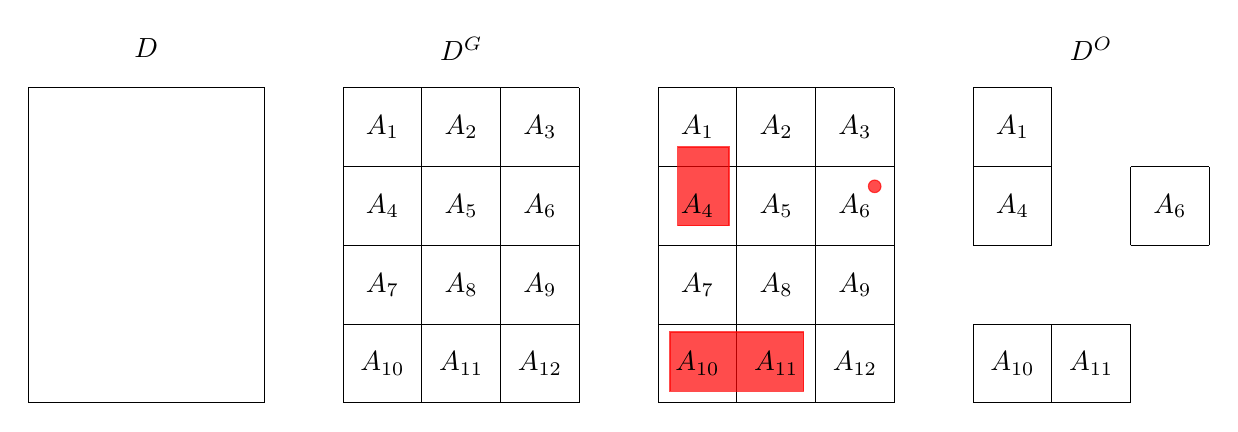
\begin{tikzpicture}
% Continuous domain D
\begin{scope}[xshift = -4cm]
\node at (1.5,4.5) {$D$};
\draw (0, 0) rectangle (3, 4);% node [below left] {$D$};
\end{scope}
% Discretised domain, D^G
\node at (1.5,4.5) {$D^G$};
\draw[step=1cm] (0,0) grid (3,4);
\node at (0.5,3.5) {$A_1$};
\node at (1.5,3.5) {$A_2$};
\node at (2.5,3.5) {$A_3$};
\node at (0.5,2.5) {$A_4$};
\node at (1.5,2.5) {$A_5$};
\node at (2.5,2.5) {$A_6$};
\node at (0.5,1.5) {$A_7$};
\node at (1.5,1.5) {$A_8$};
\node at (2.5,1.5) {$A_9$};
\node at (0.5,0.5) {$A_{10}$};
\node at (1.5,0.5) {$A_{11}$};
\node at (2.5,0.5) {$A_{12}$};
% Discretised domain, D_G, with observations
\begin{scope}[xshift = 4cm]
% \node at (1.5,4.5) {$D^O$};
\draw[step=1cm] (0,0) grid (3,4);
\filldraw[color=red, fill=red, opacity = 0.7] (0.25, 3.25) rectangle (0.9, 2.25);
\filldraw[color=red, fill=red, opacity = 0.7] (0.15, 0.15) rectangle (1.85, 0.9);
\filldraw[red, opacity = 0.7] (2.75,2.75) circle (0.08cm);
\node at (0.5,3.5) {$A_1$};
\node at (1.5,3.5) {$A_2$};
\node at (2.5,3.5) {$A_3$};
\node at (0.5,2.5) {$A_4$};
\node at (1.5,2.5) {$A_5$};
\node at (2.5,2.5) {$A_6$};
\node at (0.5,1.5) {$A_7$};
\node at (1.5,1.5) {$A_8$};
\node at (2.5,1.5) {$A_9$};
\node at (0.5,0.5) {$A_{10}$};
\node at (1.5,0.5) {$A_{11}$};
\node at (2.5,0.5) {$A_{12}$};
\end{scope}
% observation supports
\begin{scope}[xshift = 8cm]
\node at (1.5,4.5) {$D^O$};
\draw[step=1cm] (0,4) grid (1,2);
\draw[step=1cm] (0,0) grid (2,1);
\draw[step=1cm] (2,2) grid (3,3);
\node at (0.5,3.5) {$A_1$};
\node at (0.5,2.5) {$A_4$};
\node at (2.5,2.5) {$A_6$};
\node at (0.5,0.5) {$A_{10}$};
\node at (1.5,0.5) {$A_{11}$};

\end{scope}
\end{tikzpicture}
\caption{A simple example demonstrating how the continuous spatial domain, $D$, is discretised into BAUs, and how the observation domain, $D^O$, is derived from the observations.
(Left panel) The continuous spatial domain, $D$.
(Centre-left panel) The spatial domain discretised into $N = 12$ BAUs. 
(Centre-right panel) The discretised domain after observing $m = 3$ observations, two of which are area-referenced, and one that is point-referenced. 
(Right panel) The observation domain, $D^O$. The observation supports that comprise $D^O$ are; $B_1 \equiv A_1 \cup A_4$ with $c_1 \equiv \{1, 4\}$;  $B_2 \equiv A_6$ with $c_2 \equiv \{6\}$; and $B_3 \equiv A_{10} \cup A_{11}$ with $c_3 \equiv \{10, 11\}$.}\label{fig:BAU_intuition}
\end{figure}

Define the observation level mean as $\vec{\mu}_Z \equiv (\E{Z_1}, \dots, \E{Z_m})^\tp$. Then, since each $B_j \in D^O$ is either a BAU or a union of BAUs, one can construct an $m\times N$ matrix 
%\begin{equation}
%\vec{C}_Z \equiv \Big(w_i\mathbb{I}(A_i \subset B_j) : i = 1, \dots, N; j = 1, \dots, m\Big),
%\end{equation}
\begin{equation}
\vec{C}_Z \equiv \Big(w_{ij}\mathbb{I}(i \in c_j) : i = 1, \dots, N; j = 1, \dots, m\Big),
\end{equation} 
where $\mathbb{I}(\cdot)$ is the indicator function, such that
\begin{equation}\label{eqn:04-01:mu_Z}
\vec{\mu}_Z = \vec{C}_Z\vec{\mu}.  
\end{equation} 
Note that \cite{FRK_paper} applied $\vec{C}_Z$ directly to $\vec{Y}$; with an identity link function, implicit in \pkg{FRK} v1, $\vec{\mu}$ and $\vec{Y}$ are equivalent.  
In \pkg{FRK} v2, the weights $w_{ij}$ may be controlled through the \code{wts} field of the BAUs object and the argument \mbox{\code{normalise\_wts}}. 
 Specifically, the \code{wts} field allows one to attribute each BAU to some proportionality constant $v_i$, $i = 1, \dots, N$, such that $w_{ij} \propto v_i$.  
 For example, if the BAUs are of unequal area, then one may wish to set $v_i = |A_i|$. 
 By default (and implicit in \pkg{FRK} v1), each $v_i$ is set to 1. 
  The argument \mbox{\code{normalise\_wts}} controls whether $\vec{C}_Z$ corresponds to a weighted sum or a weighted average. If set to \code{FALSE}, then $w_{ij} = v_i$ for all $j$; if set to \mbox{\code{TRUE}} (default, and implicit in \pkg{FRK} v1), then $w_{ij}$ are normalised so that each row of $\vec{C}_Z$ sums to 1.  
  Note that if $v_i = |A_i|$ and \mbox{\code{normalise\_wts = TRUE}}, the $j$th row sum of $\vec{C}_Z$ is $\sum_{i \in c_j} |A_i| = |B_j|$, so that the normalised weights are $w_{ij} = |A_i|/|B_j|$.  
% The argument \mbox{\code{normalise\_wts}} controls whether $\vec{C}_Z$ corresponds to a weighted sum or a weighted average; if set to \mbox{\code{TRUE}} (default, and implicit in \pkg{FRK} v1), then the weights $w_{ij}$ are normalised so that each row of $\vec{C}_Z$ sums to 1, and the mapping represents a weighted average.  
%  Note that if $v_i = |A_i|$ and \mbox{\code{normalise\_wts = TRUE}}, the $j$th row sum of $\vec{C}_Z$ is $\sum_{i \in c_j} |A_i| = |B_j|$, so that the normalised weights are $w_{ij} = |A_i|/|B_j|$.  

 


Denoting the mean of $Z_j$, that is, the $j$th element of $\vec{\mu}_Z$, by $\vec{\mu}_{Zj}$, we assume that 
\begin{equation}\label{eqn:Z_j|mu(.)}
[Z_j \mid \mu(\cdot), \psi] = \text{EF}(\vec{\mu}_{Zj}, \psi),
\end{equation}
where EF corresponds to a probability distribution in the exponential family with dispersion parameter $\psi$, and, for generic random quantities $A$ and $B$, $[A \mid B]$ denotes the probability distribution of $A$ given $B$. 
 We assume that $\psi$ is spatially invariant, and note that $\psi = 1$ for some distributions in the exponential family (e.g., binomial, negative-binomial, and Poisson distributions). 
Equation (\ref{eqn:Z_j|mu(.)}) implies that a given observation depends only on the value of the mean process at the corresponding observation support, rather than on the process over the whole domain. 
Further, we assume that, all observations are conditionally independent given the latent spatial process:
\[
[\vec{Z} \mid \mu(\cdot), \psi] = [\vec{Z} \mid \vec{\mu}_Z, \psi] = \prod_{j=1}^m \text{EF}(\vec{\mu}_{Zj}, \psi).
\]
As we only consider data models in the exponential family, $\ln{[\vec{Z}  \mid  \vec{\mu}_Z, \psi]}$ may be expressed as  
\begin{equation}\label{eqn:ln[Z|Y],ExpFam}
\ln{[\vec{Z} \mid \vec{\mu}_Z, \psi]}
=
\sum_{j=1}^m\left\{
\frac{Z_j\lambda(\vec{\mu}_{Zj}) - b(\lambda(\vec{\mu}_{Zj}))}{a(\psi)} + c(Z_j, \psi)\right\},
\end{equation}
where $a(\cdot)$, $b(\cdot)$, and $c(\cdot, \cdot)$ are deterministic functions specific to the exponential family member, and $\lambda(\cdot)$ is the canonical parameter.
%We model the conditional distribution $[Z_j \mid \vec{\mu}_{Zj}, \psi]$ as a member of the exponential family \citep[Sec.~2.2.2]{McCullagh_Nelder_1989_GLM}, with conditional expectation $\mu(B_j) \equiv \ECurly{Z_j \mid \vec{\mu}_{Zj}, \psi}$.  

Note that two distributions catered for by \pkg{FRK} v2, namely the binomial and negative-binomial distributions, have a known constant `size' parameter, $k_j$, and a `probability of success' parameter, $\pi_j$, associated with each datum, $Z_j$; see Appendix \ref{sec:Distributions with size parameters} for details on how we link the latent process $Y(\cdot)$ to the mean process $\mu(\cdot)$ when these distributions are chosen. 
 

The model employed by \pkg{FRK} v2 can be summarised as follows. 
\begin{gather}
    Z_j \mid \vec{\mu}_{Zj}, \psi \inddist \text{EF}(\vec{\mu}_{Zj}, \psi), \quad j = 1, \dots, m, \label{eqn:new_model_Z}\\
    \vec{\mu}_Z = \vec{C}_Z \vec{\mu}, \label{eqn:new_model_muZ}\\
    g(\vec{\mu}) = \vec{Y}, \\
    \vec{Y} = \vec{T} \vec{\alpha} + \vec{S} \vec{\eta} + \vec{\xi}, \label{eqn:new_model_Y}\\
    \vec{\eta} \mid \vec{\vartheta} \sim \Gau(\vec{0}, \vec{Q}^{-1}), \\
    \vec{\xi} \mid \sigma^2_\xi \sim \Gau(\vec{0}, \sigma^2_\xi \vec{V}) \label{eqn:new_model_priors}.
%    \vec{\xi} \mid \vec{\sigma}^2_\xi \sim \Gau(\vec{0}, \vec{\Sigma}_{\xi}) \label{eqn:new_model_priors},
\end{gather}
%where $\vec{\Sigma}_{\xi}$ is a diagonal matrix, and is equal to $\sigma^2_\xi \vec{V}$ in a spatial setting, where $\vec{V}$ is a known diagonal matrix with positive entries on the diagonal and $\sigma^2_\xi$ is either unknown and estimated or provided by the user. In a spatio-temporal setting, a more complex model of $\vec{\Sigma}_{\xi}$ is allowed, although $\vec{\Sigma}_{\xi}$ is still diagonal (see Section \ref{sec:spatio-temporal}).
 where $\vec{V}$ is a known, positive-definite diagonal matrix and $\sigma^2_\xi$ is either unknown and estimated, or provided by the user. In a spatio-temporal setting, a more complex model for $\vec{\xi}$ is allowed; see Section \ref{sec:spatio-temporal}. 
 Note that \pkg{FRK} v2 is backward compatible: An identity link function and a Gaussian data model yields the model used in \pkg{FRK} v1. 



%Figure \ref{fig:02-02:DAG} shows the directed acyclic graph (DAG) of the model (\ref{eqn:new_model_Z} -- \ref{eqn:new_model_priors}). 
% In practice, we do not explicitly fit the model (\ref{eqn:new_model_Z}) -- (\ref{eqn:new_model_priors}), but rather an equivalent and more stable version. See Appendix \ref{appendix:implementation_details} for details.

%\begin{figure}[t!]
%\centering
%\resizebox{0.6\linewidth}{!}{%
%\begin{tikzpicture}[
%roundnode/.style={circle, draw=black},
%diamondnode/.style={diamond, draw=black, aspect = 2
%},
%]
%% Y field
%% \begin{scope}[shift={(0,-3)}]
%    \draw plot [scale=0.7, smooth cycle] coordinates {(0,-2.5) (-2,-3.5) (-3.8,-3.8) (-5.2, -2.5) (-4.8, -1) (-4, 0) (-2, 0.8) (0,1.3) (2,2) (4,1.3) (4.5, 0.6) (3.5, -1.5) (1,-2)} node (YField) at (1.5, -0.4) {\scriptsize $Y(\cdot)$};
%% \end{scope}
%
%% s_i
%\filldraw[black] (-3,-0.7) circle (1.5pt) node[anchor=north] (si) {\tiny $B_i$};
%\node[diamondnode] (musi) [above=of si] {\tiny $\mu(B_i)$};
%\node[roundnode] (Zsi) [above=of musi] {\tiny $Z_i$};
%\draw[->] (si.north) -- (musi.south);
%\draw[->] (musi.north) -- (Zsi.south);
%% s_j
%\filldraw[black] (-0.3,0.3) circle (1.5pt) node[anchor=north] (sj) {\tiny $B_j$};
%\node[diamondnode] (musj) [above=of sj] {\tiny $\mu(B_j)$};
%\node[roundnode] (Zsj) [above=of musj] {\tiny $Z_j$};
%\draw[->] (sj.north) -- (musj.south);
%\draw[->] (musj.north) -- (Zsj.south);
%\end{tikzpicture}
%}
%\caption[Graphical representation (DAG) of the spatial model]{Graphical representation of the spatial model outlined in Section \ref{subsection:04-02:DataLayer}. 
%First, we assume there exists a latent, correlated random field $Y(\cdot)$ permeating throughout the spatial domain $D$. 
%The value of the process $Y(\cdot)$ at any given location determines the value of the mean of the data, $\mu(\cdot)$, at that location. 
%Specifically the mean is a \textit{deterministic} function of the latent process (emphasised by the diamond shape of the conditional mean nodes). 
%Then, the distribution of the data, which is a member of the exponential family, depends on the mean at that location. 
%Finally, given the value of the latent process at $B_i$, the observation $Z_i$ is conditionally independent of both $Z_j$ and the latent process at $B_j$. }\label{fig:02-02:DAG}
%\end{figure} 


%\subsection{Inference on the process and parameter estimation}\label{subsection:02-03:Estimation}
\subsection{Estimation}\label{subsection:02-03:Estimation}

We now derive the likelihood functions required for model fitting, describe the intractable integrals that arise when using non-Gaussian data models are dealt with, and describe how \pkg{TMB} \citep{Kristensen_2016_TMB} is used to obtain estimates of the parameters/fixed effects, and predictions of the random effects.


%\subsubsection{Complete-data likelihood}

%Noting that $\vec{\mu}_Z$ is completely determined by $\vec{\mu}$, which in turn is completely determined by $\vec{Y}$, which in turn is completely determined by $\vec{\alpha}$, $\vec{\eta}$, and $\vec{\xi}$,  
Noting that $\vec{\mu}_Z$ is, through (\ref{eqn:new_model_muZ})--(\ref{eqn:new_model_Y}), completely determined by $\vec{\alpha}$, $\vec{\eta}$, and $\vec{\xi}$,  
 the complete-data likelihood function for our model is
\begin{equation}\label{eqn:04:Joint_Likelihood}
    L(\vec{\theta}; \vec{Z}, \vec{\eta}, \vec{\xi})
    \equiv 
    [\vec{Z}, \vec{\eta}, \vec{\xi} \mid \vec{\theta}]
    =
    [\vec{Z} \mid \vec{\mu}_Z, \psi]
    [\vec{\eta} \mid \vec{\vartheta}]
    [\vec{\xi} \mid \sigma^2_\xi], 
\end{equation}
 where $
 \vec{\theta}
 \equiv
 (
 \vec{\alpha}^\tp,
 \vec{\vartheta}^\tp, 
 \sigma^2_\xi, 
 \psi
 )^\tp$ and $\vec{\vartheta}$ denotes the variance components associated with either $\vec{K}$ or $\vec{Q}$.
The complete-data log-likelihood function, $l(\vec{\theta}; \vec{Z}, \vec{\eta}, \vec{\xi})$, is simply the logarithm of (\ref{eqn:04:Joint_Likelihood}). %, 
%\begin{equation}\label{eqn:04:Joint_Log_Likelihood}
%    l(\vec{\theta}; \vec{Z}, \vec{\eta}, \vec{\xi}) 
%    \equiv 
%    \ln{L(\vec{\theta}; \vec{Z}, \vec{\eta}, \vec{\xi})}
%    =
%    \ln{[\vec{Z} \mid \vec{\mu}_Z, \psi]}
%    +
%    \ln{[\vec{\eta} \mid \vec{\vartheta}]}
%    +
%    \ln{[\vec{\xi} \mid \sigma^2_\xi]}.
%\end{equation}
Under our modelling assumptions (\ref{eqn:new_model_Z})--(\ref{eqn:new_model_priors}), the conditional density functions  $[\vec{\eta}\mid\vec{\vartheta}]$ and $[\vec{\xi} \mid \sigma^2_\xi]$ are invariant to the specified link function and the assumed distribution of the response variable. 
 Of course, this invariance does not hold for $[\vec{Z} \mid \vec{\mu}_Z, \psi]$. %; see (\ref{eqn:ln[Z|Y],ExpFam}). 


%\subsubsection{Marginal likelihood}\label{sec:marginal_likelihood}

The marginal likelihood, which depends on the observations $\vec{Z}$ and not on the unobserved random effects $\vec{u} \equiv (\vec{\eta}^\tp, \vec{\xi}^\tp)^\tp$, is given by integrating out $\vec{u}$ from (\ref{eqn:04:Joint_Likelihood}):
\begin{equation}\label{eqn:02-04:LikelihoodTheta}
    L^*(\vec{\theta}; \vec{Z}) 
    \equiv
    \int_{\mathbb{R}^{{p}}}
    L(\vec{\theta} ; \vec{Z}, \vec{u}) \d \vec{u}, 
%    =
%    \int_{\mathbb{R}^{{p}}}
%    \exp\left\{l(\vec{\theta} ; \vec{Z}, \vec{u})\right\} \d \vec{u},
\end{equation}
where ${p}$ is the total number of random effects in the model.
When the data are non-Gaussian, the integral in (\ref{eqn:02-04:LikelihoodTheta}) is typically intractable and must be approximated either numerically or analytically. 
In \pkg{FRK} v2, we use a Laplace approximation, which we now describe. 


Let $\hat{\vec{u}}\equiv\hat{\vec{u}}(\vec{\theta}, \vec{Z})$ be a mode of $l(\vec{\theta}; \vec{Z}, \vec{u})$ with respect to $\vec{u}$, 
% \begin{equation*}
% \left.\nabla_{\vec{u}} l(\vec{\theta} ; \vec{Z}, \vec{u})\right\rvert_{\vec{u}=\hat{\vec{u}}} = \vec{0},
% \end{equation*}
 and let %$\vec{H}$ be the negative of the inverse Hessian matrix of $l(\vec{\theta} ; \vec{Z}, \vec{u})$ with respect to $\vec{u}$, evaluated at $\hat{\vec{u}}$:
\begin{equation*}
    \vec{H} 
    \equiv
    -\left(\left.\nabla_{\vec{u}} \nabla_{\vec{u}} l(\vec{\theta} ; \vec{Z}, \vec{u}) \right\rvert_{\vec{u}=\hat{\vec{u}}}\right)^{-1},
\end{equation*}
 where $\nabla_{\vec{u}}$ denotes the gradient with respect to $\vec{u}$. 
 A second-order Taylor series approximation of $l(\vec{\theta} ; \vec{Z}, \vec{u})$ about $\vec{u} =  \hat{\vec{u}}$ results in an approximation of %the complete-data likelihood function 
 (\ref{eqn:04:Joint_Likelihood})
 that is Gaussian in terms of $\vec{u}$, with mean vector $\hat{\vec{u}}$ and covariance matrix $\vec{H}$. 
 Substituting this approximation into (\ref{eqn:02-04:LikelihoodTheta}) 
 and evaluating the integral 
 yields the Laplace approximation of the marginal likelihood, $L^*(\vec{\theta}; \vec{Z})
    \approx L(\vec{\theta} ; \vec{Z}, \hat{\vec{u}})
    (2\pi)^{\frac{{p}}{2}}\left|\vec{H}\right|^{\frac{1}{2}}$.
% This allows $\vec{u}$ to be integrated out of $L(\vec{\theta}; \vec{Z}, \vec{u})$, yielding the Laplace approximation of the marginal log likelihood, $l^*(\vec{\theta}; \vec{Z}) \approx l(\vec{\theta} ;  \vec{Z}, \hat{\vec{u}}) + \frac{{p}}{2} \ln{2\pi} + \frac{1}{2} \ln{\left|\vec{H}\right|}$.
 
 
 Note that $[\vec{u} \mid \vec{Z}, \vec{\theta}] \propto [\vec{u}, \vec{Z} \mid \vec{\theta}]$, and $[\vec{u}, \vec{Z} \mid \vec{\theta}]$ is equal to the complete-data likelihood function, $L(\vec{\theta}; \vec{Z}, \vec{u})$. 
 Since the Laplace approximation replaces $L(\vec{\theta}; \vec{Z}, \vec{u})$ with a term that has the form of a Gaussian distribution, $\Gau(\hat{\vec{u}}, \vec{H})$, in terms of $\vec{u}$, it follows that, approximately, $\vec{u} \mid \vec{Z}, \vec{\theta} \sim \Gau(\hat{\vec{u}}, \vec{H})$. 
  Further, \pkg{TMB} \citep[][see below]{Kristensen_2016_TMB} provides estimates of $\hat{\vec{u}}$ and $\vec{H}^{-1}$. 
This makes prediction of $\vec{u}$ and nonlinear functions of $\vec{u}$ via MC simulation straightforward; see Section \ref{subsection:04-03:Prediction}. 


%Using a second-order Taylor series approximation of $l(\vec{\theta} ; \vec{Z}, \vec{u})$ about $\red{\vec{u} =} \hat{\vec{u}}$, the Laplace approximation of the marginal likelihood is
%\begin{align*}
%    L^*(\vec{\theta}; \vec{Z})
%    \approx L(\vec{\theta} ; \vec{Z}, \hat{\vec{u}})
%    (2\pi)^{\frac{{p}}{2}}\left|\vec{H}\right|^{\frac{1}{2}},
%\end{align*}
%and so the Laplace approximation of the marginal log likelihood is 
%\begin{equation}\label{eqn:02-04:Laplace_margloglike}
%l^*(\vec{\theta}; \vec{Z})
%    \approx
%    l(\vec{\theta} ;  \vec{Z}, \hat{\vec{u}}) + \frac{{p}}{2} \log{2\pi} + \frac{1}{2} \log{\left|\vec{H}\right|}.
%\end{equation}
%Therefore, the Laplace approximation makes the assumption that the conditional distribution of the random effects is Gaussian with mean vector $\hat{\vec{u}}$ and variance matrix $\vec{H}$; that is, $\vec{u} \mid \vec{Z}, \vec{\theta} \sim \Gau(\hat{\vec{u}}, \vec{H})$.
%This makes prediction of $\vec{u}$ and nonlinear functions of $\vec{u}$ via MC straightforward. 





%%%%%%%%%%%% LONGER VERSION
 
%\red{Longer version} 
% 
% Let $\vec{u} \equiv (\vec{\eta}^\tp, \vec{\xi}^\tp)^\tp \in \mathbb{R}^{{p}}$ denote the random effects in our model, where ${p}$ is the total number of random effects.
% The marginal likelihood function, $L^*(\vec{\theta}; \vec{Z})$, is obtained by integrating out the random effects from the complete-data likelihood function;
% \begin{equation}\label{eqn:02-04:LikelihoodTheta}
%     L^*(\vec{\theta}; \vec{Z}) 
%     = 
%     \int_{\mathbb{R}^{{p}}}
%     L(\vec{\theta} ; \vec{Z}, \vec{u}) \d \vec{u} 
%     \equiv 
%     \int_{\mathbb{R}^{{p}}}
%     \exp\left\{l(\vec{\theta} ; \vec{Z}, \vec{u})\right\} \d \vec{u}.
% \end{equation}
%  When the data model is non-Gaussian, this integral is intractable and requires either numerical or analytical approximation.
%  The Laplace approximation involves approximating $ L(\vec{\theta} ; \vec{Z}, \vec{u})$ with a Gaussian distribution centred at a mode of $ L(\vec{\theta} ; \vec{Z}, \vec{u})$.
% Define $\hat{\vec{u}}\equiv\hat{\vec{u}}(\vec{\theta}, \vec{Z})$ to be a mode of $l(\vec{\theta}; \vec{Z}, \vec{u})$ with respect to $\vec{u}$.
%  \begin{equation*}
%  \left.\nabla_{\vec{u}} l(\vec{\theta} ; \vec{Z}, \vec{u})\right\rvert_{\vec{u}=\hat{\vec{u}}} = \vec{0},
%  \end{equation*}
%  where $\nabla_{\vec{u}}$ denotes the gradient with respect to $\vec{u}$.
% A second-order Taylor series approximation of $l(\vec{\theta} ; \vec{Z}, \vec{u})$ about $\hat{\vec{u}}$ yields
% \begin{equation}\label{eqn:02-04:TaylorApprox}
% l(\vec{\theta} ; \vec{Z}, \vec{u}) 
%     \approx 
%     l(\vec{\theta} ; \vec{Z}, \hat{\vec{u}}) 
%     -
%     \frac{1}{2}(\vec{u} - \hat{\vec{u}})^\tp \vec{H}^{-1}(\vec{u} - \hat{\vec{u}}), 
% \end{equation}
% where 
%  the first-order term is zero as we have expanded about a stationary point, and 
% $\vec{H}$ is the negative of the inverse Hessian matrix of $l(\vec{\theta} ; \vec{Z}, \vec{u})$ with respect to $\vec{u}$ at $\hat{\vec{u}}$:
% \begin{equation*}
%     \vec{H} = \vec{H}(\vec{\theta}; \vec{Z})
%     =
%     -\left(\left.\nabla_{\vec{u}} \nabla_{\vec{u}} l(\vec{\theta} ; \vec{Z}, \vec{u}) \right\rvert_{\vec{u}=\hat{\vec{u}}}\right)^{-1}.
% \end{equation*}
% Exponentiating (\ref{eqn:02-04:TaylorApprox}), we have that
% \begin{equation}\label{eqn:approx_joint_likelihood}
%     L(\vec{\theta} ; \vec{Z}, \vec{u}) 
%     \approx 
%     L(\vec{\theta} ; \vec{Z}, \hat{\vec{u}}) \exp\left\{
%     -
%     \frac{1}{2}(\vec{u} - \hat{\vec{u}})^\tp \vec{H}^{-1}(\vec{u} - \hat{\vec{u}})
%     \right\},
% \end{equation}
% while substituting (\ref{eqn:approx_joint_likelihood}) into the marginal likelihood (\ref{eqn:02-04:LikelihoodTheta}) yields the Laplace approximation of the marginal likelihood:
% \begin{align*}
%     L^*(\vec{\theta}; \vec{Z})
%      &= \int_{\mathbb{R}^{{p}}} L(\vec{\theta} ; \vec{Z}, \vec{u}) \d \vec{u}\\
%      &= \int_{\mathbb{R}^{{p}}} \exp\left\{l(\vec{\theta} ; \vec{Z}, \vec{u})\right\} \d \vec{u}\\
%     &\approx \int_{\mathbb{R}^{{p}}} L(\vec{\theta} ; \vec{Z}, \hat{\vec{u}}) \exp\left\{
%     -
%     \frac{1}{2}(\vec{u} - \hat{\vec{u}})^\tp \vec{H}^{-1}(\vec{u} - \hat{\vec{u}})
%     \right\} \d \vec{u}\\
%      &= L(\vec{\theta} ; \vec{Z}, \hat{\vec{u}})\int_{\mathbb{R}^{{p}}} \exp\left\{-\frac{1}{2}(\vec{u} - \hat{\vec{u}})^\tp \vec{H}^{-1} (\vec{u} - \hat{\vec{u}})\right\} \d \vec{u}\\
%      &= L(\vec{\theta} ; \vec{Z}, \hat{\vec{u}})
%      \left|2\pi\vec{H}\right|^{\frac{1}{2}}\\
%     &= L(\vec{\theta} ; \vec{Z}, \hat{\vec{u}})
%     (2\pi)^{\frac{{p}}{2}}\left|\vec{H}\right|^{\frac{1}{2}}.
% \end{align*}
%  Hence, the Laplace approximation of the marginal likelihood is
%  \begin{equation}\label{eqn:02-04:marglike}
%      L^*(\vec{\theta}; \vec{Z})
%      \approx
%      L(\vec{\theta} ; \hat{\vec{u}}, \vec{Z})
%      (2\pi)^{\frac{s}{2}}\left|\vec{H}\right|^{\frac{1}{2}}.
%  \end{equation}
% The Laplace approximation of the marginal log-likelihood is then
% \begin{equation}\label{eqn:02-04:margloglike}
% l^*(\vec{\theta}; \vec{Z}) = 
%     \ln{L^*(\vec{\theta}; \vec{Z})}
%     \approx
%     l(\vec{\theta} ;  \vec{Z}, \hat{\vec{u}}) + \frac{{p}}{2} \log{2\pi} + \frac{1}{2} \log{\left|\vec{H}\right|}.
% \end{equation}
%
%% % The reason for $\hat{\vec{u}}$ needing to be a mode (rather than the weaker condition of it being a stationary point) is apparent: in order for the Gaussian density function used to derive the approximation to be well defined (and integrate to one), its variance-covariance matrix must be positive definite, which implies that $\hat{\vec{u}}$ must be a maximum (i.e., a mode of the log-likelihood function). 
%
%% % As an aside, a maximum likelihood estimate of the parameters derived from (\ref{eqn:02-04:margloglike}) is the maximum of the function $L^*(\vec{\theta}; \vec{Z})$ with respect to the parameters $\vec{\theta}$; it is, in general, \textit{not} the maximum of $L(\vec{\theta}; \vec{Z}, \vec{u})$. This is a subtle yet important distinction; see Figure \ref{fig:02-04:TwoProbMass} for further clarification.  
%
% The Laplace approximation implicitly assumes the posterior distribution of the random effects is Gaussian.  
%  we may express the complete-data  likelihood function as
%  \begin{align*}
%      L(\vec{\theta}; \vec{Z}, \vec{u})
%      &= 
%      [\vec{Z}, \vec{u} \mid \vec{\theta}]
%      =
%      [\vec{u} \mid \vec{Z}, \vec{\theta}][\vec{Z} \mid \vec{\theta}],
%  \end{align*}
% To see this, substituting the complete-data likelihood function with its Laplace approximation, we have that
% \begin{align*}
%     [\vec{u} \mid \vec{Z}, \vec{\theta}]
%     &=
%     \frac{L(\vec{\theta}; \vec{Z}, \vec{u})}{[\vec{Z} \mid \vec{\theta}]}\\
%     &\approx 
%     \frac{L(\vec{\theta} ; \vec{Z}, \hat{\vec{u}}) }{[\vec{Z} \mid \vec{\theta}]}\exp\left\{
%     -
%     \frac{1}{2}(\vec{u} - \hat{\vec{u}})^\tp \vec{H}^{-1}(\vec{u} - \hat{\vec{u}})
%     \right\}\\
%     &\propto
%     \exp\left\{
%     -
%     \frac{1}{2}(\vec{u} - \hat{\vec{u}})^\tp \vec{H}^{-1}(\vec{u} - \hat{\vec{u}})
%     \right\},
% \end{align*}
% so that (approximately) $\vec{u} \mid \vec{Z}, \vec{\theta} \sim \Gau(\hat{\vec{u}}, \vec{H})$.
%


% \subsubsection{The Laplace approximation using \pkg{TMB}}

\subsubsection[Model fitting with TMB]{Model fitting with \pkg{TMB}}

Given a \proglang{C++} template function that defines $l(\vec{\theta} ; \vec{Z}, \vec{u})$, \pkg{TMB} \citep{Kristensen_2016_TMB} computes the Laplace approximation of the log marginal likelihood, and automatically computes its derivatives. These quantities are then called from within \pkg{FRK} v2 by an optimising function specified by the user (\fct{nlminb} is used by default). 
 \pkg{TMB} uses \pkg{CppAD} \citep{CppAD_Package} for automatic differentiation, and the linear algebra libraries \pkg{Eigen} \citep{Eigen} and \pkg{Matrix} \citep{Matrix_Package} for vector and matrix operations in \proglang{C++} and \proglang{R}, respectively; use of these packages yields very good computational efficiency. 
\pkg{TMB}'s implementation of automatic differentiation is a key reason why \pkg{FRK} v2 can cater for a variety of response distributions and link functions, as each combination does not need to be considered on a case-by-case basis.

Note that all parameters, fixed effects, and random effects, are treated as random in \pkg{TMB} (with a flat prior assumed if a prior is not provided).
We fix the parameters and fixed effects to their posterior-mode estimates, and then treat them as non-random quantities.% when doing prediction. 

%Note that all parameters, fixed effects, and random effects, are treated as random in \pkg{TMB} (with a flat prior assumed if a prior is not provided).
%We fix the parameters to their posterior-mode estimates and then treat them as non-random quantities when doing prediction; however, we let the user decide if the fixed effects $\vec{\alpha}$ are treated as fixed or random. 
%If they fixed, flagged by setting \code{kriging = "simple"} in the function \fct{predict}, they are treated in the same way as the parameters. 
%If they are random, we jointly sample $\vec{\alpha}$ along with the random effects $\vec{u}$ in the prediction stage;  this choice accounts for the uncertainty in estimation of $\vec{\alpha}$, and so it is flagged by setting \code{kriging = "universal"} (see \red{Cressie (1993, Ch. 3) OR AN EARLIER REFERENCE THAT IS IN THAT CHAPTER} for the equivalence of using a flat prior on $\vec{\alpha}$ to performing universal kriging). 


%%%%% Notes which are useful to keep, but do not need to be in the paper:

%The justification for fixing the parameters/fixed-effects to their mode estimators is as follows. 
%\pkg{TMB} uses the Laplace approximation, and so implicitly assumes that
%\begin{equation}
%    \begin{bmatrix}
%    \vec{\theta} \\
%    \vec{u}
%    \end{bmatrix}
%    \sim \Gau\left( 
%    \begin{bmatrix}
%    \hat{\vec{\theta}} \\
%    \hat{\vec{u}}
%    \end{bmatrix}, 
%    \begin{bmatrix}
%    \vec{Q}_{\theta, \theta} & \vec{Q}_{\theta, u} \\
%    \vec{Q}_{u, \theta} & \vec{Q}_{u, u}
%    \end{bmatrix}^{-1}
%    \right).
%\end{equation}
%If we fix $\vec{\theta}$ to their mode estimates, that is, if we condition on $\vec{\theta} = \hat{\vec{\theta}}$, then,
%by well known properties of the Gaussian distribution \citep[e.g., ][App. A]{RW_2006_Gaussian_Processes_for_Machine_Learning}, we have that 
%$\ENoLR{\vec{u} \mid \vec{\theta} = \hat{\vec{\theta}}} = \hat{\vec{u}}$
%and
%$\precisionNoLR{\vec{u} \mid \vec{\theta} =  \hat{\vec{\theta}}} = \vec{Q}_{u, u}$.


\subsection{Prediction and uncertainty quantification}\label{subsection:04-03:Prediction}

%% NB: A longer form of the prediction section, which also discusses analytic solutions, is commented out in the appendices


%%The MSPE has an appealing form when the conditional expectation, $\E{A \mid \vec{Z}}$, is used as a predictor of some quantity $A$; specifically, using the law of total expectation, and the definition of conditional variance, it can be shown that
%%% \begin{align}\label{eqn:04-03:GeneralMSPE}
%%%     \MSPEtwoarg{\E{A \mid \vec{Z}}}{A}
%%%     &\equiv
%%%     \ESquare{\left\{\E{A \mid \vec{Z}}-A\right\}^2} \nonumber \\
%%%     &=
%%%     \ESquare{\E{\left\{\E{A \mid \vec{Z}}-A\right\}^2 \mathrel{\Big|} \vec{Z}}} \nonumber \\
%%%     &=
%%%     \ESquare{\var{A \mid \vec{Z}}}.
%%%     %= \var{A} - \varCurly{\E{A \mid \vec{Z}}},
%%% \end{align}
%%\begin{equation}\label{eqn:04-03:GeneralMSPE}
%%    \MSPEtwoarg{\E{A \mid \vec{Z}}}{A}
%%    \equiv
%%    \ESquare{\left\{\E{A \mid \vec{Z}}-A\right\}^2} 
%%    % =
%%    % \ESquare{\E{\left\{\E{A \mid \vec{Z}}-A\right\}^2 \mathrel{\Big|} \vec{Z}}}
%%    =
%%    \ECurly{\var{A \mid \vec{Z}}},
%%\end{equation}
%%where $\MSPEtwoarg{\cdot}{\cdot}$ is a function of two arguments (the predictor, and the predictand). 
%%If $A$ and $\vec{Z}$ are both Gaussian, then $A \mid \vec{Z}$ exhibits a feature known as conditional homoskedasticity; that is, the conditional variance $\var{A \mid \vec{Z}}$ \textit{does not} depend on $\vec{Z}$ \citep[e.g., ][p.~110]{Cressie_1993_stats_for_spatial_data}. 
%%In this case, (\ref{eqn:04-03:GeneralMSPE}) is equal to  $\var{A \mid \vec{Z}}$. 
%%When the conditional variance \textit{does} depend on $\vec{Z}$, (\ref{eqn:04-03:GeneralMSPE}) can be estimated by dropping the expectation. 
%% Then the MSPE (\ref{eqn:04-03:GeneralMSPE}) is given by
%% \begin{equation}\label{eqn:04-03:MSPEyGivenz2}
%%     \MSPEtwoarg{\pYgivenZ{\vec{s}_0}}{Y(\vec{s}_0)} 
%%     \approx 
%%     \varCurly{Y(\vec{s}_0) \mid \vec{Z}, \vec{\theta}},
%% \end{equation}
%% where approximate equality is replaced by equality in the case of Gaussian data. 


%We now discuss prediction, and quantifying the uncertainty of those predictions. 
%There are three primary quantities of interest in this framework: The latent process $Y(\cdot)$, the  mean process $\mu(\cdot)$, and the noisy data process. 
%For each quantity, we use the posterior expectation as our predictor. % ; a decision theoretic justification for this choice is provided by \citet*[ch.~3]{Cressie_1993_stats_for_spatial_data}.
%
%The predictor of $Y_i$, the latent process $Y(\cdot)$ evaluated over the BAU $A_i$, is
%\begin{equation}\label{eqn:02-03:pYgivenZ}
%    \pYgivenZ{A_i}
%    \equiv
%    \ECurly{Y_i \mid \vec{Z}, \vec{\theta}}.
%\end{equation}
%Recall from Section 
%\ref{subsection:02-03:Estimation} 
% that the Laplace approximation implies that the posterior distribution of the random effects, $\vec{u} \equiv (\vec{\eta}^\tp, \vec{\xi}^\tp)^\tp$, is approximated to be Gaussian. 
% This, in turn, implies that the posterior distribution of $Y_i$ is also approximated to be Gaussian, and (\ref{eqn:02-03:pYgivenZ}) is available in closed form. 
% However, the posterior distribution of non-linear functions of $Y_i$ (e.g., the mean process) are typically not available in closed form, and in this case some form of approximation is required. 
%  Hence, with an eye to prediction of the mean process, we choose to use MC sampling to compute (\ref{eqn:02-03:pYgivenZ}). 
%
%Denote the posterior mode and precision matrix of the random effects by $\hat{\vec{u}}$ and $\vec{Q}_{u}$, respectively. These quantities are estimated using \pkg{TMB}. 
%%
%%Define a permuted version of the precision matrix as $\vec{A} \equiv \vec{P}^\tp \vec{Q}_{u} \vec{P}$, where $\vec{P}$ is a permutation matrix. Define the upper Cholesky factor of $\vec{A}$ as $\vec{U}_P$, which is the upper triangular matrix satisfying $\vec{A} = \vec{U}_P^\tp \vec{U}_P$. Then, we have that $\vec{Q}_{u} = \vec{M}^\tp \vec{M}$, where $\vec{M} = \vec{U}_P \vec{P}^\tp$ is \textit{not} triangular.
%%Now consider the usual method of transforming a standard Gaussian vector to a Gaussian vector with precision matrix $\vec{Q}_{u}$. 
%%First, let $\vec{z} \sim \Gau(\vec{0}, \vec{I})$ denote a standard Gaussian random vector. Then, we have that the variance of the transformed vector $\tilde{\vec{u}} \equiv \vec{M}^{-1}\vec{z} $ is
%%\begin{align*}
%%    \var{\tilde{\vec{u}}}
%%    = \var{\vec{M}^{-1}\vec{z}}
%%    = \vec{M}^{-1}\vec{M}^{-\tp}
%%    = (\vec{M}^{\tp}\vec{M})^{-1}
%%    = \vec{Q}_{u}^{-1},
%%\end{align*}
%%as required. Note, however, that although $\vec{M}$ is sparse, it is not triangular.
%%However, we have that $\vec{M}^{-1} = \vec{P} \vec{U}_P^{-1}$,
%%and so $\tilde{\vec{u}}$ may equivalently be written as
%%$\tilde{\vec{u}} = \vec{P} \vec{U}_P^{-1}\vec{z}$.
%%Therefore, we can first solve the upper triangular system $\vec{U}_P \vec{x} = \vec{z}$, and then left-multiply $\vec{x}$ by the permutation matrix $\vec{P}$ to obtain $\tilde{\vec{u}} = \vec{P} \vec{x} = \vec{P} \vec{U}_P^{-1}\vec{z} = \vec{M}^{-1}\vec{z}$, as required. 
%%This approach to generating samples fully exploits both the reduction of fill-in from matrix reordering, as well as a computationally efficient backward-solve.
%%
%Let $\vec{Y}_{\!\text{MC}}$ be an $N \times n_{\text{MC}}$ matrix whose columns are MC samples of $\vec{Y} \mid \vec{Z}, \vec{\theta}$. 
% If \code{kriging = "simple"} we construct $\vec{Y}_{\!\text{MC}}$ via 
%\begin{equation}\label{eqn:Y_MC_simple}
%\vec{Y}_{\!\text{MC}}
%\equiv \vec{T}\vec{A} + [\vec{S} \; \vec{I}] \,\vec{U},
%\end{equation}
%where $\vec{A}$ is a $q \times n_{\text{MC}}$ matrix whose columns consist of the estimated posterior mode of $\vec{\alpha}$ (and where $q$ denotes the dimension of $\vec{\alpha}$), and $\vec{U}$ is a $p \times n_{\text{MC}}$ matrix whose columns are MC samples of $\vec{u} \mid \vec{Z}, \vec{\theta}$. 
% If \code{kriging = "universal"}, then $\vec{\alpha}$ are treated as random effects and included in $\vec{u}$, and (\ref{eqn:Y_MC_simple}) is rewritten as
% \begin{equation}\label{eqn:Y_MC_universal}
%\vec{Y}_{\!\text{MC}}
%\equiv [\vec{T} \; \vec{S} \; \vec{I}] \,\vec{U},
%\end{equation}
%where $\vec{U}$ is now a $(p + q) \times n_{\text{MC}}$ matrix and includes samples of $\vec{\alpha} \mid \vec{Z}, \vec{\theta}$. We estimate (\ref{eqn:02-03:pYgivenZ}) for $i = 1, \dots, N$ by simply taking row-wise averages of $\vec{Y}_{\!\text{MC}}$. 
% 
%After construction of $\vec{Y}_{\!\text{MC}}$, prediction of the mean process $\mu(\cdot)$ proceeds straightforwardly. The predictor of $\mu_i$, the mean process evaluated the BAU $A_i$, is
%\begin{equation}\label{eqn:04-03:muOptimalPredictor}
%    \pmugivenZ{A_i} 
%    \equiv 
%    \ECurly{\mu_i \mid \vec{Z}, \vec{\theta}} = \ECurly{g^{-1}(Y_i) \mid \vec{Z}, \vec{\theta}}.
%\end{equation}
%We obtain MC samples of $\vec{\mu}$ via $\vec{M} \equiv g^{-1}(\vec{Y}_{\!\text{MC}})$, where $g^{-1}(\cdot)$ is applied element-wise. Computation of (\ref{eqn:04-03:muOptimalPredictor}) then simply involves row-wise averaging of $\vec{M}$.
% 
%We now turn our attention to prediction and prediction uncertainty of the noisy data process. 
%Again, we use the posterior expectation as our predictor, 
%\begin{equation}\label{eqn:04-03:ZOptimalPredictor}
%    \hat{p}_{Z_i|\vec{Z}}
%    \equiv 
%    \ECurly{Z_i \mid \vec{Z}, \vec{\theta}},
%\end{equation}
%which, using the law of total expectation, can be shown to be equivalent to (\ref{eqn:04-03:muOptimalPredictor}).  
% MC samples of the noisy data process can be constructed straightforwardly using $\vec{M}$, since the distribution of an exponential family member depends only on its conditional mean (and a dispersion parameter, which me model as being constant throughout the spatial domain). 


We now discuss spatial prediction, and uncertainty quantification of the predictions. 
There are three possible quantities of interest in this framework: The latent process $Y(\cdot)$, the  mean process $\mu(\cdot)$, and the noisy data process. 
% To produce predictions and associated uncertainties, we need to determine the posterior distribution of these quantities.
%For each quantity, we use the posterior expectation as our predictor. % ; a decision theoretic justification for this choice is provided by \citet*[ch.~3]{Cressie_1993_stats_for_spatial_data}.
Recall  
%from Section \ref{subsection:02-03:Estimation} 
 that the Laplace approximation implies that, approximately, $\vec{u} \mid \vec{Z}, \vec{\theta} \sim \Gau(\hat{\vec{u}}, \vec{H})$; since $\vec{Y}$ is a linear function of $\vec{u}$, inference on $Y(\cdot)$ can hence be done using closed form solutions. 
  However, the posterior distribution of non-linear functions of $Y(\cdot)$ (e.g., the mean process) are typically not available in closed form, and some type of approximation is required.
   We choose to use a MC framework.
%  Hence, with an eye to inference on the mean process, we choose to use a MC framework to estimate the posterior distribution of $\vec{Y}$.


%The predictor of $Y_i$, the latent process $Y(\cdot)$ evaluated over the BAU $A_i$, is
%\begin{equation}\label{eqn:02-03:pYgivenZ}
%    \pYgivenZ{A_i}
%    \equiv
%    \ECurly{Y_i \mid \vec{Z}, \vec{\theta}}.
%\end{equation}


%Denote the posterior mode and precision matrix of the random effects by $\hat{\vec{u}}$ and $\vec{Q}_{u}$, respectively. These quantities are estimated using \pkg{TMB}. 
%
%Define a permuted version of the precision matrix as $\vec{A} \equiv \vec{P}^\tp \vec{Q}_{u} \vec{P}$, where $\vec{P}$ is a permutation matrix. Define the upper Cholesky factor of $\vec{A}$ as $\vec{U}_P$, which is the upper triangular matrix satisfying $\vec{A} = \vec{U}_P^\tp \vec{U}_P$. Then, we have that $\vec{Q}_{u} = \vec{M}^\tp \vec{M}$, where $\vec{M} = \vec{U}_P \vec{P}^\tp$ is \textit{not} triangular.
%Now consider the usual method of transforming a standard Gaussian vector to a Gaussian vector with precision matrix $\vec{Q}_{u}$. 
%First, let $\vec{z} \sim \Gau(\vec{0}, \vec{I})$ denote a standard Gaussian random vector. Then, we have that the variance of the transformed vector $\tilde{\vec{u}} \equiv \vec{M}^{-1}\vec{z} $ is
%\begin{align*}
%    \var{\tilde{\vec{u}}}
%    = \var{\vec{M}^{-1}\vec{z}}
%    = \vec{M}^{-1}\vec{M}^{-\tp}
%    = (\vec{M}^{\tp}\vec{M})^{-1}
%    = \vec{Q}_{u}^{-1},
%\end{align*}
%as required. Note, however, that although $\vec{M}$ is sparse, it is not triangular.
%However, we have that $\vec{M}^{-1} = \vec{P} \vec{U}_P^{-1}$,
%and so $\tilde{\vec{u}}$ may equivalently be written as
%$\tilde{\vec{u}} = \vec{P} \vec{U}_P^{-1}\vec{z}$.
%Therefore, we can first solve the upper triangular system $\vec{U}_P \vec{x} = \vec{z}$, and then left-multiply $\vec{x}$ by the permutation matrix $\vec{P}$ to obtain $\tilde{\vec{u}} = \vec{P} \vec{x} = \vec{P} \vec{U}_P^{-1}\vec{z} = \vec{M}^{-1}\vec{z}$, as required. 
%This approach to generating samples fully exploits both the reduction of fill-in from matrix reordering, as well as a computationally efficient backward-solve.



%Recall that $\vec{Y} = \vec{T}\vec{\alpha} + \vec{S}\vec{\eta} + \vec{\xi}$. 
% If \code{kriging = "simple"}, then $\vec{u} = (\vec{\eta}^\tp, \vec{\xi}^\tp)^\tp$ and $\vec{Y} = \vec{T}\vec{\alpha} + [\vec{S} \; \vec{I}] \,\vec{u}$, so we construct $\vec{Y}_{\!\text{MC}}$ via
 Recall that $\vec{u} \equiv (\vec{\eta}^\tp, \vec{\xi}^\tp)^\tp$ and that $\vec{Y} = \vec{T}\vec{\alpha} + \vec{S}\vec{\eta} + \vec{\xi}$, which can be rewritten as $\vec{Y} = \vec{T}\vec{\alpha} + [\vec{S} \; \vec{I}] \,\vec{u}$. 
 We thus define $\vec{Y}_{\!\text{MC}}$, an $N \times n_{\text{MC}}$ matrix whose columns are MC samples of $\vec{Y} \mid \vec{Z}, \vec{\theta}$, as 
\begin{equation}\label{eqn:Y_MC_simple}
\vec{Y}_{\!\text{MC}}
\equiv \vec{T}\vec{A} + [\vec{S} \; \vec{I}] \,\vec{U},
\end{equation}
where each of the $n_{\text{MC}}$ columns of the matrix $\vec{A}$ contain the estimated posterior mode of $\vec{\alpha}$, %is a $q \times n_{\text{MC}}$ matrix whose columns consist of the estimated posterior mode of $\vec{\alpha}$ %(and where $q$ denotes the dimension of $\vec{\alpha}$), 
% and $\vec{U}$ is a matrix with $n_{\text{MC}}$ columns consisting of MC samples of $\vec{u} \mid \vec{Z}, \vec{\theta}$.  
  and each of the $n_{\text{MC}}$ columns of the matrix $\vec{U}$ are draws from  $\vec{u} \mid \vec{Z}, \vec{\theta} \sim \Gau(\hat{\vec{u}}, \vec{H})$.  
% If \code{kriging = "universal"}, then $\vec{\alpha}$ are treated as random effects and included in $\vec{u}$, and (\ref{eqn:Y_MC_simple}) is rewritten as
% \begin{equation}\label{eqn:Y_MC_universal}
%\vec{Y}_{\!\text{MC}}
%\equiv [\vec{T} \; \vec{S} \; \vec{I}] \,\vec{U},
%\end{equation}
%where $\vec{U}$ %is now a $(p + q) \times n_{\text{MC}}$ matrix that 
%now 
%also includes samples of $\vec{\alpha} \mid \vec{Z}, \vec{\theta}$. 
 We obtain MC samples of $\vec{\mu} \mid \vec{Z}, \vec{\theta}$ via $\vec{M} \equiv g^{-1}(\vec{Y}_{\!\text{MC}})$, where $g^{-1}(\cdot)$ is applied element-wise. Finally, MC samples of the noisy data process can be constructed straightforwardly using $\vec{M}$, since the distribution of an exponential family member depends only on its conditional mean (and a dispersion parameter, which we model as being constant throughout the spatial domain). 

For each quantity, we use the posterior expectation as our predictor, which can be estimated by simply taking row-wise averages of the matrices defined above. 
In a Gaussian setting, a commonly used metric for uncertainty quantification is the root-mean-squared prediction error (RMSPE). 
In a non-Gaussian setting, it can be difficult to interpret the RMSPE, and it is often more intuitive to quantify uncertainty through the width of the posterior predictive intervals. Hence, in \pkg{FRK} v2, we also use the MC sampling approach described above to compute user-specified percentiles of the posterior predictive distribution.  

 
%After construction of $\vec{Y}_{\!\text{MC}}$, prediction of the mean process $\mu(\cdot)$ proceeds straightforwardly. The predictor of $\mu_i$, the mean process evaluated the BAU $A_i$, is
%\begin{equation}\label{eqn:04-03:muOptimalPredictor}
%    \pmugivenZ{A_i} 
%    \equiv 
%    \ECurly{\mu_i \mid \vec{Z}, \vec{\theta}} = \ECurly{g^{-1}(Y_i) \mid \vec{Z}, \vec{\theta}}.
%\end{equation}
%Computation of (\ref{eqn:04-03:muOptimalPredictor}) then simply involves row-wise averaging of $\vec{M}$.
 
%We now turn our attention to prediction and prediction uncertainty of the noisy data process. 
%Again, we use the posterior expectation as our predictor, 
%\begin{equation}\label{eqn:04-03:ZOptimalPredictor}
%    \hat{p}_{Z_i|\vec{Z}}
%    \equiv 
%    \ECurly{Z_i \mid \vec{Z}, \vec{\theta}},
%\end{equation}
%which, using the law of total expectation, can be shown to be equivalent to (\ref{eqn:04-03:muOptimalPredictor}).  
 




\subsubsection{Arbitrary prediction regions}


Often, one does not wish to predict over a single BAU, but over regions spanning multiple BAUs.
Define the set of prediction regions as 
$D^P \equiv \{\tilde{B}_k : k = 1, \dots, N_P\}$, where $\tilde{B}_k \equiv \cup_{i\in c_k} A_i$, and where $\tilde{c}_k$ is some non-empty set in the power set of $\{1, \dots, N\}$. 
%Here, $N_P$ is the number of areas at which spatial prediction takes place, and is equal to $|D^P|$.
Like the observation supports, the prediction regions $\{\tilde{B}_k\}$ may overlap, and, in practice, may not include entire BAUs; our criteria for determining whether a prediction region contains a BAU is the same as that used for determining whether an observation support contains a BAU (see Section \ref{subsection:04-02:DataLayer}). 


Prediction over $D^P$ requires some form of aggregation across relevant BAUs.
Since aggregation must be done on the response scale, we restrict prediction over arbitrary regions to the mean process (or the noisy data process).  
% \red{(Can we predict noisy data process over aggregations of the BAUs? Does it require assuming permanence of whatever-distribution-we-are-using?)}
%In particular, predictions of the latent process $Y(\cdot)$ are not allowed over arbitrary prediction regions.
%Consider the process $\{\mu_P(\tilde{B}_k) : k = 1, \dots, N_P\}$, which is derived from the mean process $\mu(\cdot)$. 
Consider $\vec{\mu}_P \equiv \{\mu(\tilde{B}_k) : k = 1, \dots, N_P\}$, the mean process evaluated over the prediction regions. Just as $\vec{\mu}_Z$ was constructed from the BAU level mean process $\vec{\mu}$ via $\vec{C}_Z$, since each $\tilde{B}_k$ is a BAU or a union of BAUs, one can construct an $N_P \times N$ matrix 
\[
\vec{C}_P \equiv \left(\tilde{w}_{i,k}\mathbb{I}(i \in \tilde{c}_k) : i = 1, \dots, N; k = 1, \dots, N_P\right),
\]
such that
\[
\vec{\mu}_P = \vec{C}_P \vec{\mu}.
\]
%Specifically,
%\[
%    \mu_{P, k} \equiv \mu_P(\tilde{B}_k) = 
%   \sum_{i = 1}^N \tilde{w}_{i,k} \mathbb{I}(A_i \subset \tilde{B}_k)\mu_i; \quad i = 1, \dots, N;\;  k = 1, \dots, N_P;\; \tilde{B}_k \in D^P.
%\]
As before, the proportionality constants, $\{v_i: i = 1, \dots, N\}$, for the weights $\{\tilde{w}_{i,k}\}$ are controlled by the \code{wts} field of the BAU object and the argument \mbox{\code{normalise\_wts}}. 
 For consistency between the model fitting and prediction stages, in \pkg{FRK} v2 we require that the same proportionality constants and the same value of \code{normalise\_wts} are used in construction of both $\vec{C}_Z$ and $\vec{C}_P$. 


 MC samples of $\vec{\mu}_P \mid \vec{Z}, \vec{\theta}$ can be constructed  via $\vec{M}_P \equiv \vec{C}_P \vec{M}$, where recall that $\vec{M}$ consists of MC samples of $\vec{\mu} \mid \vec{Z}, \vec{\theta}$. Predictions and uncertainty quantification of the predictions can then be computed straightforwardly. 
 
%We typically use MC sampling to predict $\vec{\mu}_P$. 
% This involves generating an $N\times n_{\text{MC}}$ matrix $\vec{M}$ whose columns are MC samples of $\vec{\mu}$. % (see Appendix \ref{app:prediction}). 
% Then, the columns of $\vec{C}_P\vec{M}$ are MC samples of $\vec{\mu}_P$.
%First, we construct $\vec{Y}_{\!\text{MC}}$, an $N \times n_{\text{MC}}$ matrix whose $i$th row contains $n_{\text{MC}}$ MC samples of $Y_i$. 
%Then, we pass these samples through the inverse link function to obtain MC samples of the mean process, $
%\vec{M} \equiv g^{-1}(\vec{Y}_{\!\text{MC}})$,
%where $g^{-1}(\cdot)$ is applied element-wise. 
%Finally, we let $
%\vec{M}_P \equiv \vec{C}_P \vec{M}$,
%whose $n_{\text{MC}}$ columns consist of MC samples of $\vec{\mu}_P$. 
%The samples contained in $\vec{M}_P$ can then be used to obtain predictions and associated prediction uncertainty of $\vec{\mu}_P$.
%If inference on the noisy data process over aggregations of BAUs is desired, \pkg{FRK} v2 returns predictions and uncertainty by simulating the specified response distribution with mean equal to the samples in $\vec{M}_P$. 



% For intuition on the preceding discussion, write the matrices $\vec{M}$ and $\vec{C}_P$ as
% \[
% \vec{M} =
% \begin{bmatrix}
% \vec{\mu}_1 & \dots & \vec{\mu}_{n_{\text{MC}}}
% \end{bmatrix},
% \]
% and 
% \[
% \vec{C}_P =
% \begin{bmatrix}
% \vec{c}_{1}^\tp \\ 
% \vdots \\
% \vec{c}_{N_P}^\tp
% \end{bmatrix},
% \]
% respectively, where
% $\vec{\mu}_j$ denotes the $j$th MC sample of $\vec{\mu}$, and $\vec{c}_{k}^\tp$ is the vector of weights associated with prediction region $\tilde{B}_k$.
% Then we have
% \[
% \vec{C}_P\vec{M}
% =
% \begin{bmatrix}
% \vec{c}_{1}^\tp \\ 
% \vdots \\
% \vec{c}_{N_P}^\tp
% \end{bmatrix}
% \begin{bmatrix}
% \vec{\mu}_1 & \dots & \vec{\mu}_{n_{\text{MC}}}
% \end{bmatrix}
% =
% \begin{bmatrix}
% \vec{c}_{1}^\tp\vec{\mu}_1 & \dots & \vec{c}_{1}^\tp\vec{\mu}_{n_{\text{MC}}}\\
% \vec{c}_{2}^\tp\vec{\mu}_1 & \dots & \vec{c}_{2}^\tp\vec{\mu}_{n_{\text{MC}}}\\
% \vdots &  & \vdots\\
% \vec{c}_{N_P}^\tp\vec{\mu}_1 & \dots & \vec{c}_{N_P}^\tp\vec{\mu}_{n_{\text{MC}}}
% \end{bmatrix}.
% \]
% Now, $\vec{c}_{k}^\tp \vec{\mu}_j$ is a scalar, and is a MC sample of the $k$th element of $\vec{\mu}_P$, and so it is not difficult to see that each of the $n_{\text{MC}}$ columns of $\vec{C}_P\vec{M}$ contain a MC of $\vec{\mu}_P$.


\subsection{Spatio-temporal framework}\label{sec:spatio-temporal}

Extending \pkg{FRK} v2 to accommodate non-Gaussian spatio-temporal data involves using an additional dimension of basis functions.
Let $r_t$ and $r_s$ denote the number of temporal and spatial basis functions, respectively. 
Denote $\vec{Q}_t$ and $\vec{Q}_s$ as the precision matrices of the random coefficients associated with the temporal basis functions and spatial basis functions, respectively. 
We model the $r_tr_s \times r_tr_s$ precision matrix  of the $r_tr_s$ spatio-temporal random coefficients associated with basis functions created through the tensor product of the $r_t$ temporal and $r_s$ spatial basis functions as
\[
\vec{Q} = \vec{Q}_t \otimes \vec{Q}_s.
\]
The assumption of separability between time and space, and hence the ability to write $\vec{Q}$ as a Kronecker product, leads to significant computational savings. 
\pkg{FRK} v2 uses an AR1 model for the random coefficients associated with the temporal basis functions.

In a spatio-temporal setting, it is possible that each spatial BAU is observed multiple times. 
Furthermore, it is also possible that the fine-scale variation is not constant over the spatial domain $D$. 
In these situations, a better fit may be obtained by allowing each spatial BAU to be associated with its own fine-scale variance parameter. 
Let $N_s$ and $N_t$ denote the number of spatial and temporal BAUs, respectively (so that $N = N_sN_t$).
Then, instead of modelling $\vec{\xi} \sim \Gau(\vec{0}, \sigma^2_\xi \vec{I})$, \pkg{FRK} v2 also allows one to model
$\vec{\xi} \sim \Gau\left(\vec{0}, \vec{\Sigma}_\xi\right)$,
where 
\begin{equation}
    \vec{\Sigma}_\xi \equiv
\begin{pmatrix}
\text{diag}(\vec{\sigma}^2_\xi) & & \\
&  \ddots  & \\
&    & \text{diag}(\vec{\sigma}^2_\xi)\\
\end{pmatrix},
\end{equation}
$\vec{\sigma}^2_\xi \equiv (\sigma^2_{\xi, 1}, \dots, \sigma^2_{\xi, N_s})^\tp$,
and the BAUs are assumed to be ordered such that space runs faster than time. 
This model for $\vec{\Sigma}_\xi$ is flagged by setting \code{fs\_by\_spatial\_BAU = TRUE} in the \fct{SRE} function, and is particularly useful when the number of spatial BAUs (and hence variance parameters to estimate) is relatively low and we have observed each spatial BAU over many time-points; see, for instance, the example presented in Section \ref{sec:ST_example}. 


\section{Usage of new features}\label{SEC:IllustrativeExample}

We now demonstrate the new features in \pkg{FRK} v2, an overview of which is presented in Table \ref{tab:new_arguments_in_functions}. 
 The primary new feature in \pkg{FRK} v2 is the packages ability to cater for non-Gaussian data models: A full list of available data models and link functions is shown in Table \ref{table:response_and_links}. 
 In Sections \ref{sec:03-01:Poisson} and \ref{sec:03-03:negative-binomial}, we illustrate use of \pkg{FRK} v2 using non-Gaussian spatial point-referenced and area-referenced data, respectively. 
% In Section \ref{sec:03:Additonal_features}, we briefly discuss extensions available in \pkg{FRK} v2 to model data in a spatio-temporal setting. 
 Finally, in Section \ref{sec:3:increased_resolution}, we show the potential improvement in predictive performance of \pkg{FRK} v2 over \pkg{FRK} v1 when the data are Gaussian, thanks to the support for an increased number of basis functions in \pkg{FRK} v2. For all results presented in the remainder of this paper, reproducible code is provided at \url{https://github.com/MattSainsbury-Dale/FRKv2_src}. 


\begin{table}
    \centering
    \setlength{\tabcolsep}{4pt}
 \caption{Important extensions to function arguments in \pkg{FRK} v2.}\label{tab:new_arguments_in_functions} 
    \begin{tabular}{ccp{9.5cm}}
    \hline
    Function & Argument & Use\\
    \hline
    \fct{SRE} & \code{response}  & A string indicating the data model. \\
        & \code{link}      & A string indicating the link function.\\
        & \code{K\_type}   & A string indicating the parameterisation of $\cov{\vec{\eta}}{\vec{\eta}}$; the newly permissible value, \code{"precision"}, specifies that a sparse precision matrix should be used. 
        \\
        & \code{normalise\_wts} & A flag controlling whether weights in $\vec{C}_Z$ and $\vec{C}_P$ should be normalised, so that aggregation of the mean corresponds either to a weighted sum or a weighted average.\\
        & \code{fs\_by\_spatial\_BAU} & A flag controlling whether each spatial BAU is given its own fine-scale variance parameter; only applicable in a spatio-temporal setting.\\
        \fct{SRE.fit} & \code{method} & A string indicating the method of model fitting; the newly permissible value, \code{"TMB"}, is required whenever a non-Gaussian data model or non-identity link function is used.\\
%        & \code{optimiser} & Optimising function if \code{method = "TMB"}; default \fct{nlminb}. \\
%        & \code{taper}     & A positive scalar indicating the strength of the covariance tapering (see Appendix \ref{Appendix:CovarianceTapering}).\\
        & \code{known\_sigma2fs} & Allows one to fix the fine-scale variance to a known value. 
%        If \code{fs\_by\_spatial\_BAU = TRUE}, the argument \code{known\_sigma2fs} should be a vector of length equal to the number of spatial BAUs.
\\
        \fct{predict} 
%        & \code{newdata} & The prediction regions; in addition to \code{Spatial*DataFrame}and \code{STFDF}, \code{newdata} can now be a \code{SpatialPoints} or \code{STI} object, facilitating prediction over spatial or spatio-temporal point-referenced locations.\\
        & \code{type} & A vector of strings indicating the quantities of interest for which inference is desired. 
%        If \code{"link"} is in \code{type}, $Y(\cdot)$ is included; if \code{"mean"} is in \code{type},  the mean process (and the probability process, if applicable) is included; if \code{"response"} is in \code{type},  the response variable is included. 
        The inclusion of \code{"link"}, \code{"mean"}, and \code{"response"} in \code{type} respectively indicate that inference on $Y(\cdot)$, $\mu(\cdot)$, or the noisy data process is desired.\\ 
        & \code{percentiles} & Numeric vector %(each element between 0 and 100) 
        indicating the percentiles of the posterior predictive distribution(s) to be computed.\\
%        & \code{kriging} & A character string indicating whether \code{"simple"} or \code{"universal"} kriging is to be performed. \\
%        & \code{k} & Vector of size parameters at each prediction location (applicable only for binomial and negative-binomial data).\\
        & \code{n\_MC} & Integer indicating the number of MC samples at each BAU.\\
        \fct{auto\_BAUs} & \code{spatial\_BAUs} & 
        The spatial BAUs in a spatio-temporal setting. If \code{NULL}, the spatial BAUs are constructed automatically.\\
%        & \code{buffer} & Numeric (between 0 and 0.5) indicating the size of the buffer of basis functions along the boundary. 
%        The buffer is added by computing the number of basis functions in each dimension, and increasing this number by a factor of \code{buffer}.
%        As precision matrices are more sensitive to boundary effects, a buffer can be useful when \code{K\_type = "precision"}.\\
\fct{plot} & - & A method for visualising the data, predictions, and uncertainty quantification of the predictions given an \class{SRE} object and the result of a call to \fct{predict} on the \class{SRE} object.\\
        \hline
    \end{tabular}
\end{table}








\begin{table}[t!]
\setlength{\tabcolsep}{6pt}
\renewcommand{\arraystretch}{1.5}
    \begin{center}
    \caption{Combinations of exponential family member response distributions and link functions available in \pkg{FRK} v2. A `\checkmark' indicates a combination is supported. A `$\bullet$' indicates a combination is allowed, however, due to the implied range of $\mu$, the support of the observations, and the form of probability density function of that family, nonsensical results are possible; if one of these problematic combinations is chosen, a warning is given to the user. Finally, blank entries indicate that the combination is not allowed.}
    \label{table:response_and_links}
    \begin{tabular}{cc|*{5}{c}|}
    \multicolumn{2}{c}{} & \multicolumn{5}{c}{\textbf{Link Function}} \\
    % Use multicolumn to remove vertical bars
     & \multicolumn{1}{c}{} & \multicolumn{1}{c}{identity} &  \multicolumn{1}{c}{inverse} & \multicolumn{1}{c}{log} & \multicolumn{1}{c}{square-root} & 
%     \multicolumn{1}{c}{\pbox{4cm}{logit/\\probit/\\cloglog}}  
\multicolumn{1}{c}{logit/probit/cloglog} 
     \\\cline{3-7} 
     % Start of Family cells
     \multirow{7}{*}{\rotatebox{90}{\textbf{Family}}} & Gaussian & \checkmark & \checkmark & $\bullet$ & $\bullet$ &  \\
      & Poisson & $\bullet$ & $\bullet$ &  \checkmark & \checkmark &  \\
      & gamma & $\bullet$ & $\bullet$ & \checkmark & \checkmark &  \\
      & inverse-Gaussian & $\bullet$ & $\bullet$ &  \checkmark & \checkmark &  \\
      & negative-binomial &  &  &   \checkmark & \checkmark & \checkmark \\
      & binomial &  &  &  &  &   \checkmark \\\cline{3-7}
    \end{tabular}
    \end{center}
%    \begin{tabnote}
%    $^{*}$The binomial and negative-binomial distributions have a known constant `size' parameter, $k_j$, and a `probability of success' parameter, $\pi_j$, associated with each datum, $Z_j$; see Appendix \ref{sec:Distributions with size parameters} for details on how we link the latent process $Y(\cdot)$ to the mean process $\mu(\cdot)$ when these distributions are chosen.
%    \end{tabnote}
\end{table}



\subsection{Example: Non-Gaussian, point-referenced spatial data}\label{sec:03-01:Poisson}
%\subsection{Non-Gaussian, point-referenced spatial data}\label{sec:03-01:Poisson}





%For illustration, and so that readers can familiarise themselves with the workflow of \pkg{FRK} v2, we use a Poisson data set containing 750 observations as a running example. 
%The data, simulated using code provided in the `Quick start' section on the \pkg{FRK} Github page (\url{https://github.com/andrewzm/FRK}), and the true field from which the data was simulated, is displayed in Figure \ref{fig:Poisson_true_and_Z}.
%For convenience, we include the data in \pkg{FRK} v2 as \code{"Poisson\_simulated"}.
%The following code loads these data and casts them into a \class{SpatialPointsDataFrame}.
%\begin{Code}
%R> library("FRK")
%R> data("Poisson_simulated")
%R> coordinates(Poisson_simulated) <- ~ x + y
%\end{Code}

For illustration, and so that readers can familiarise themselves with the workflow of \pkg{FRK} v2, we now analyse a simulated Poisson data set containing 750 observations. 
The true mean process over $D$ and the data are shown in Figure \ref{fig:Poisson_true_and_Z}.
%For convenience, we include the data in \pkg{FRK} v2 as \code{"Poisson\_simulated"}.
%The following code loads these data and casts them into a \class{SpatialPointsDataFrame}.
%\begin{Code}
%R> library("FRK")
%R> data("Poisson_simulated")
%R> coordinates(Poisson_simulated) <- ~ x + y
%\end{Code}




\begin{figure}[t!]
    \centering
    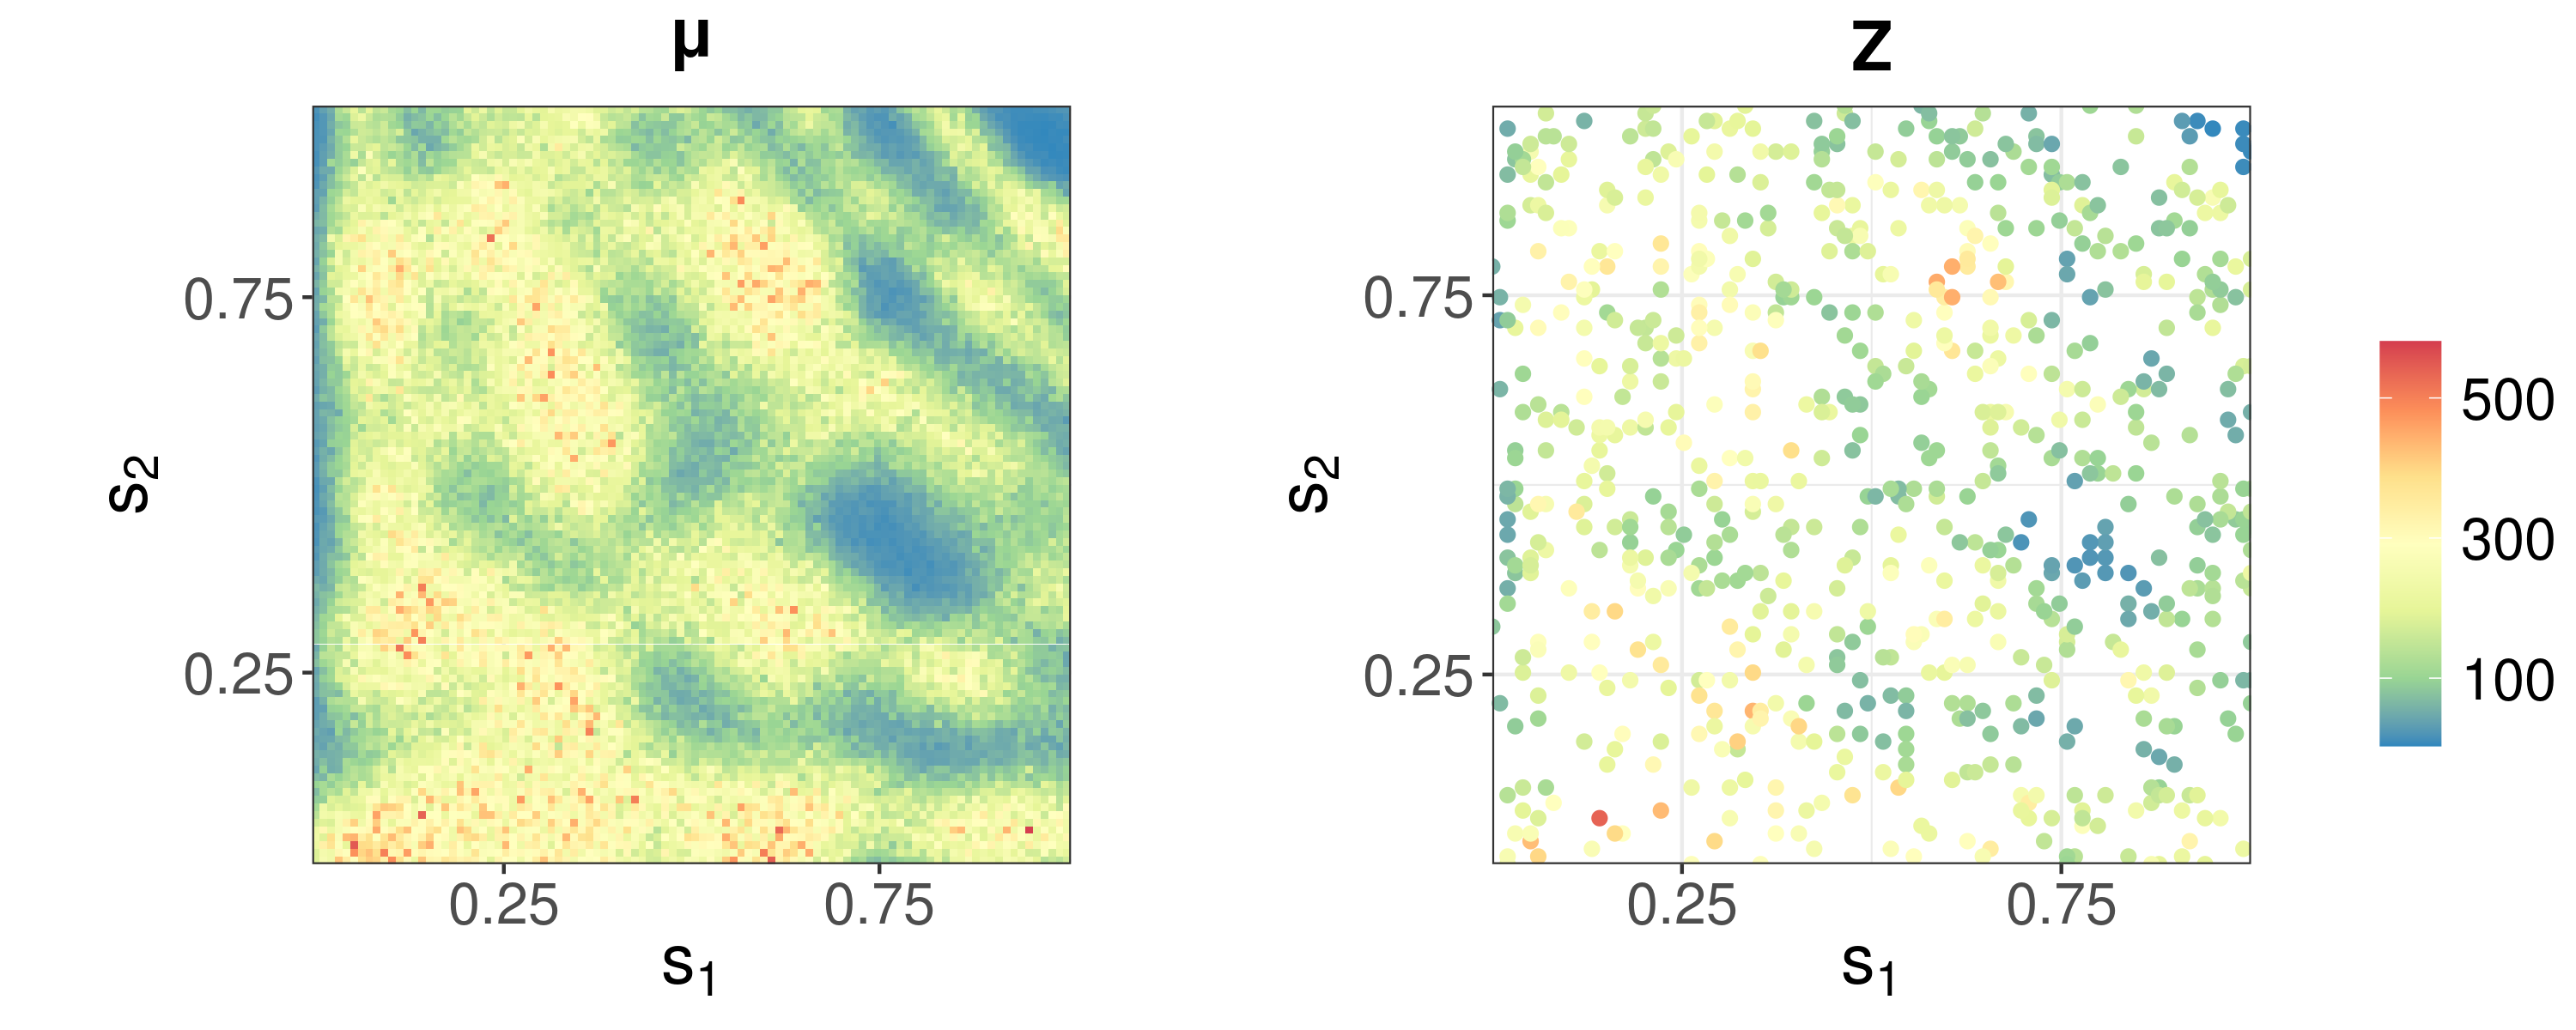
\includegraphics[width = 0.75\linewidth]{img/Poisson_sim_true_process_and_data.png}
    \caption{Simulated point-referenced spatial Poisson data set, and the true field from which the data was generated, used for the example presented in Section \ref{sec:03-01:Poisson}. (Left Panel) True mean process $\mu(\cdot)$. (Right panel) Simulated observations.  
}   
  \label{fig:Poisson_true_and_Z}
\end{figure}


%\subsubsection{Model fitting}

The first step when using \pkg{FRK} v1/v2 is to create basis functions and BAUs, which can be done automatically using the helper functions \fct{auto\_BAUs} and \fct{auto\_basis}; see \cite{FRK_paper} for details. 
Next, an \class{SRE} object is initialised using \fct{SRE}, within which we specify the data model, the link function, %(in this example, we use \code{response = "poisson"} and \code{link = "log"}), 
 and the parameterisation of $\cov{\vec{\eta}}{\vec{\eta}}$.  %the basis-function coefficients. 
%In this example, as we are using a non-Gaussian data model, we must use \code{method = "TMB"} for model fitting; \pkg{TMB} is more computationally efficient when using a sparse precision matrix, so we set \code{K\_type = "precision"}.
 We fit the model using \fct{SRE.fit}.
 These steps may be performed in a single line of code with the convenient wrapper function \fct{FRK}. Note that when the data are non-Gaussian or a non-identity link function is chosen, \fct{FRK} automatically selects
%  \code{method = "TMB"} and 
 \code{K\_type = "precision"}.
\begin{Code}
R> S <- FRK(f = Z ~ 1, data = list(Poisson_simulated),
+    response = "poisson", link = "log")
\end{Code}
%\subsubsection{Prediction}
Prediction is done using \fct{predict}. 
The argument \code{type} specifies the quantities of interest for which predictions and uncertainty quantification of the predictions are desired. 
In this example, we set \code{type = c("link", "mean")} to obtain predictions for the latent process $Y(\cdot)$ and the mean process $\mu(\cdot)$. 
The \code{percentiles} argument allows the computation of percentiles of the posterior predictive distributions, and hence posterior predictive intervals; by default, the 5th and 95th percentiles are computed.
\begin{Code}
R> pred <- predict(S, type = c("link", "mean"))
\end{Code}
When \code{method = "TMB"}, the returned object is a \class{list} containing two elements. 
The first element is an object of the same class as \code{newdata} (if \code{newdata} is unspecified, prediction is done over the BAUs), and contains the predictions and uncertainty quantification of the predictions for each term in \code{type}.
The second element is a \class{list} of matrices containing MC samples for each term in \code{type} at each prediction location. Finally, we can generate a \class{list} of \class{ggplot} \citep{Wickham_2016_ggplot2} objects of the predictions and associated uncertainty using the function \fct{plot}. 
\begin{Code}
R> plots <- plot(S, pred$newdata)
\end{Code}
The \class{ggplot} objects can then easily be arranged in a grid using various dedicated packages; we used \pkg{ggpubr} \citep{Kassambara_2020_ggpubr}. Figure \ref{fig:Poisson_nres3} shows prediction and uncertainty quantification of the predictions for the latent process $Y(\cdot)$ and the mean process $\mu(\cdot)$. 
The predictions of $\mu(\cdot)$ are reasonable given the data and the true process shown in Figure \ref{fig:Poisson_true_and_Z}. 
The prediction uncertainty for $Y(\cdot)$ is relatively flat, with uncertainty increasing in regions of data paucity; on the other hand, the prediction uncertainty for $\mu(\cdot)$ is roughly proportional to its prediction. 
The  `bullseye' points of low uncertainty, visible for both processes, correspond to the observed locations. 
The point-like nature of this reduction in uncertainty arises from the fine-scale random effects, $\vec{\xi}$, being modelled as mutually independent at the BAU level: unobserved BAUs do not borrow strength from the inferred fine-scale random effect at neighbouring observed BAUs.
\begin{figure}[t!]
    \centering
    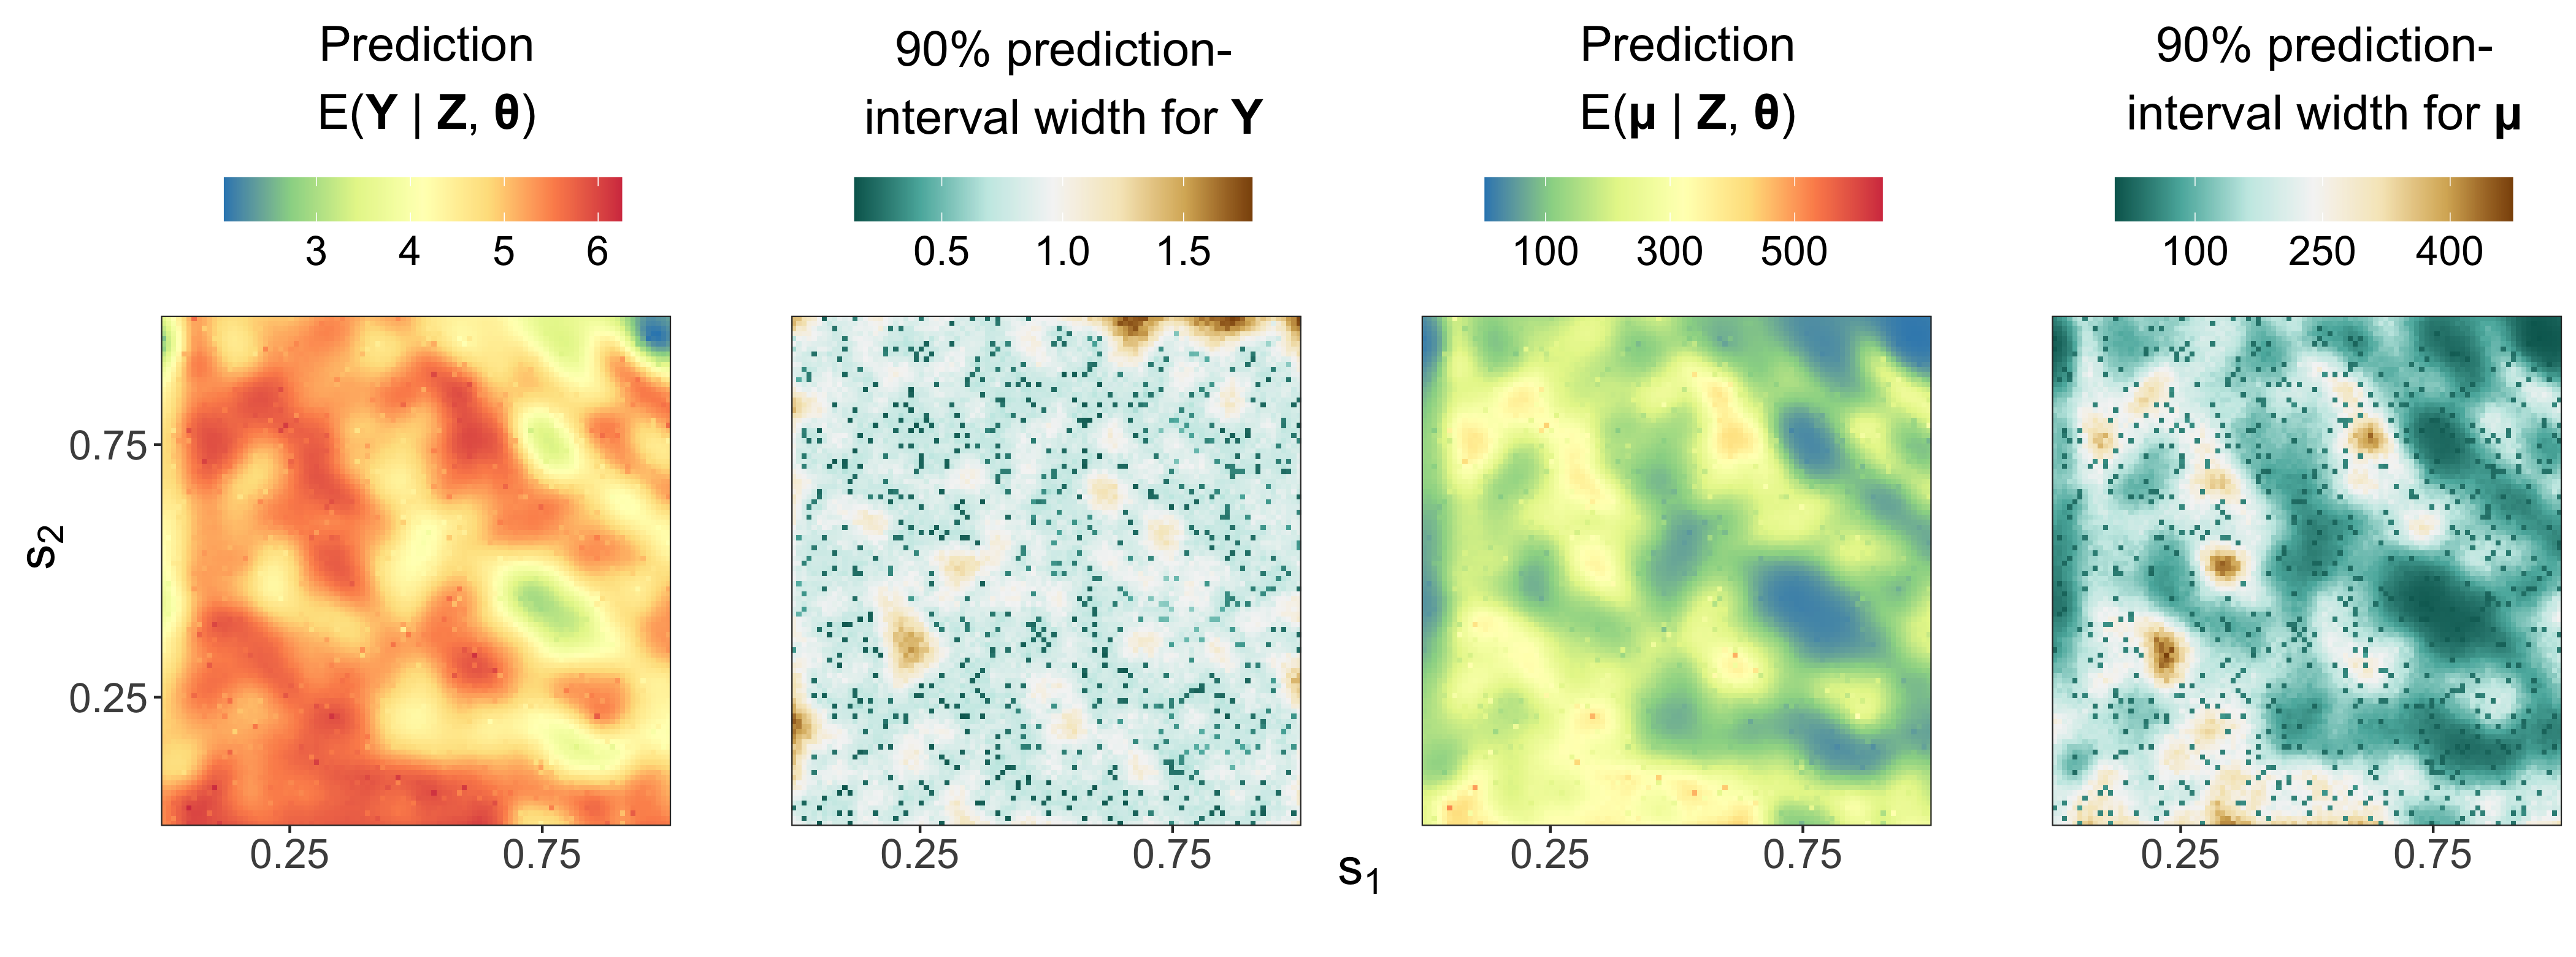
\includegraphics[width = \linewidth]{img/Poisson_sim.png}
    \caption{The prediction and prediction uncertainty quantification using the data shown in Figure \ref{fig:Poisson_true_and_Z}. (Left panel) Prediction of the latent process, $Y(\cdot)$. (Centre-left panel) Width of the 90\% central predictive interval of the latent process. (Centre-right panel) Prediction of the mean process, $\mu(\cdot)$ . (Right panel) Width of the 90\% central predictive interval of the mean process. 
}   
  \label{fig:Poisson_nres3}
\end{figure}








\subsection{Example: Non-Gaussian, areally-referenced spatial data and change of support}\label{sec:03-03:negative-binomial}



In this section, we illustrate \pkg{FRK} v2 on simulated negative-binomial, areally-referenced, spatial data, as well as its use in predicting over large areas. 

%First, we define two square grids; the first is at a fine-resolution, and corresponds to the BAUs, whilst the second is at a coarser resolution, and corresponds to areal observation supports. 
%To simulate data, we define a probability process in our domain of interest by passing a sum of trigonometric functions through the logistic function, and then evaluating it over the BAUs. 
%Once the probability process over the BAUs is defined, we then construct the mean process evaluated over the BAUs. 
% As we are simulating negative-binomial data, construction of the mean requires specification of a size parameter; for simplicity, we use $k = 50$ for each BAU.
%We then aggregate the mean process at the BAU level over the larger data support level.
%Then, we simulate our observations using the aggregated mean process. 
%Finally, we exclude some observations to form a training set.
%This process of data simulation is illustrated in Figure \ref{fig:03-02-negative-binomial_data}, and the code is provided on the \href{https://github.com/andrewzm/FRK}{\pkg{FRK} Github page}. 
%At the end of the data simulation stage, we have two \class{SpatialPolygonsDataFrame} objects, \code{BAUs} and \code{zdf}, which contain the BAUs and the observations, respectively.
 
 
In the the first step of data simualtion, we define two square grids: The first is at a fine resolution and corresponds to the BAUs, and the second is at a coarser resolution and corresponds to areal data supports. 
 To get a handle on the fine-scale variation parameter, we use some of the BAUs as data supports: Hence we have a mixture of coarse- and fine-scale observations. 
We define the probability process evaluated over the BAUs by passing a sum of trigonometric functions through the logistic function. 
We then construct the mean process evaluated over the BAUs; as we are simulating negative-binomial data, this requires specification of a size parameter, and for simplicity we use $k = 50$ for each BAU.
We then sum the mean process over the data supports, and simulate data using the aggregated mean process. 
Finally, we exclude some observations to form a training set. 
 This simulation procedure is illustrated in Figure \ref{fig:03-02-negative-binomial_data}. 
%We are left with two 
%%\class{SpatialPolygonsDataFrame} 
%objects, \code{BAUs} and \code{zdf}, which contain the BAUs and the observations, respectively. 


\begin{figure}[t!]
    \centering
    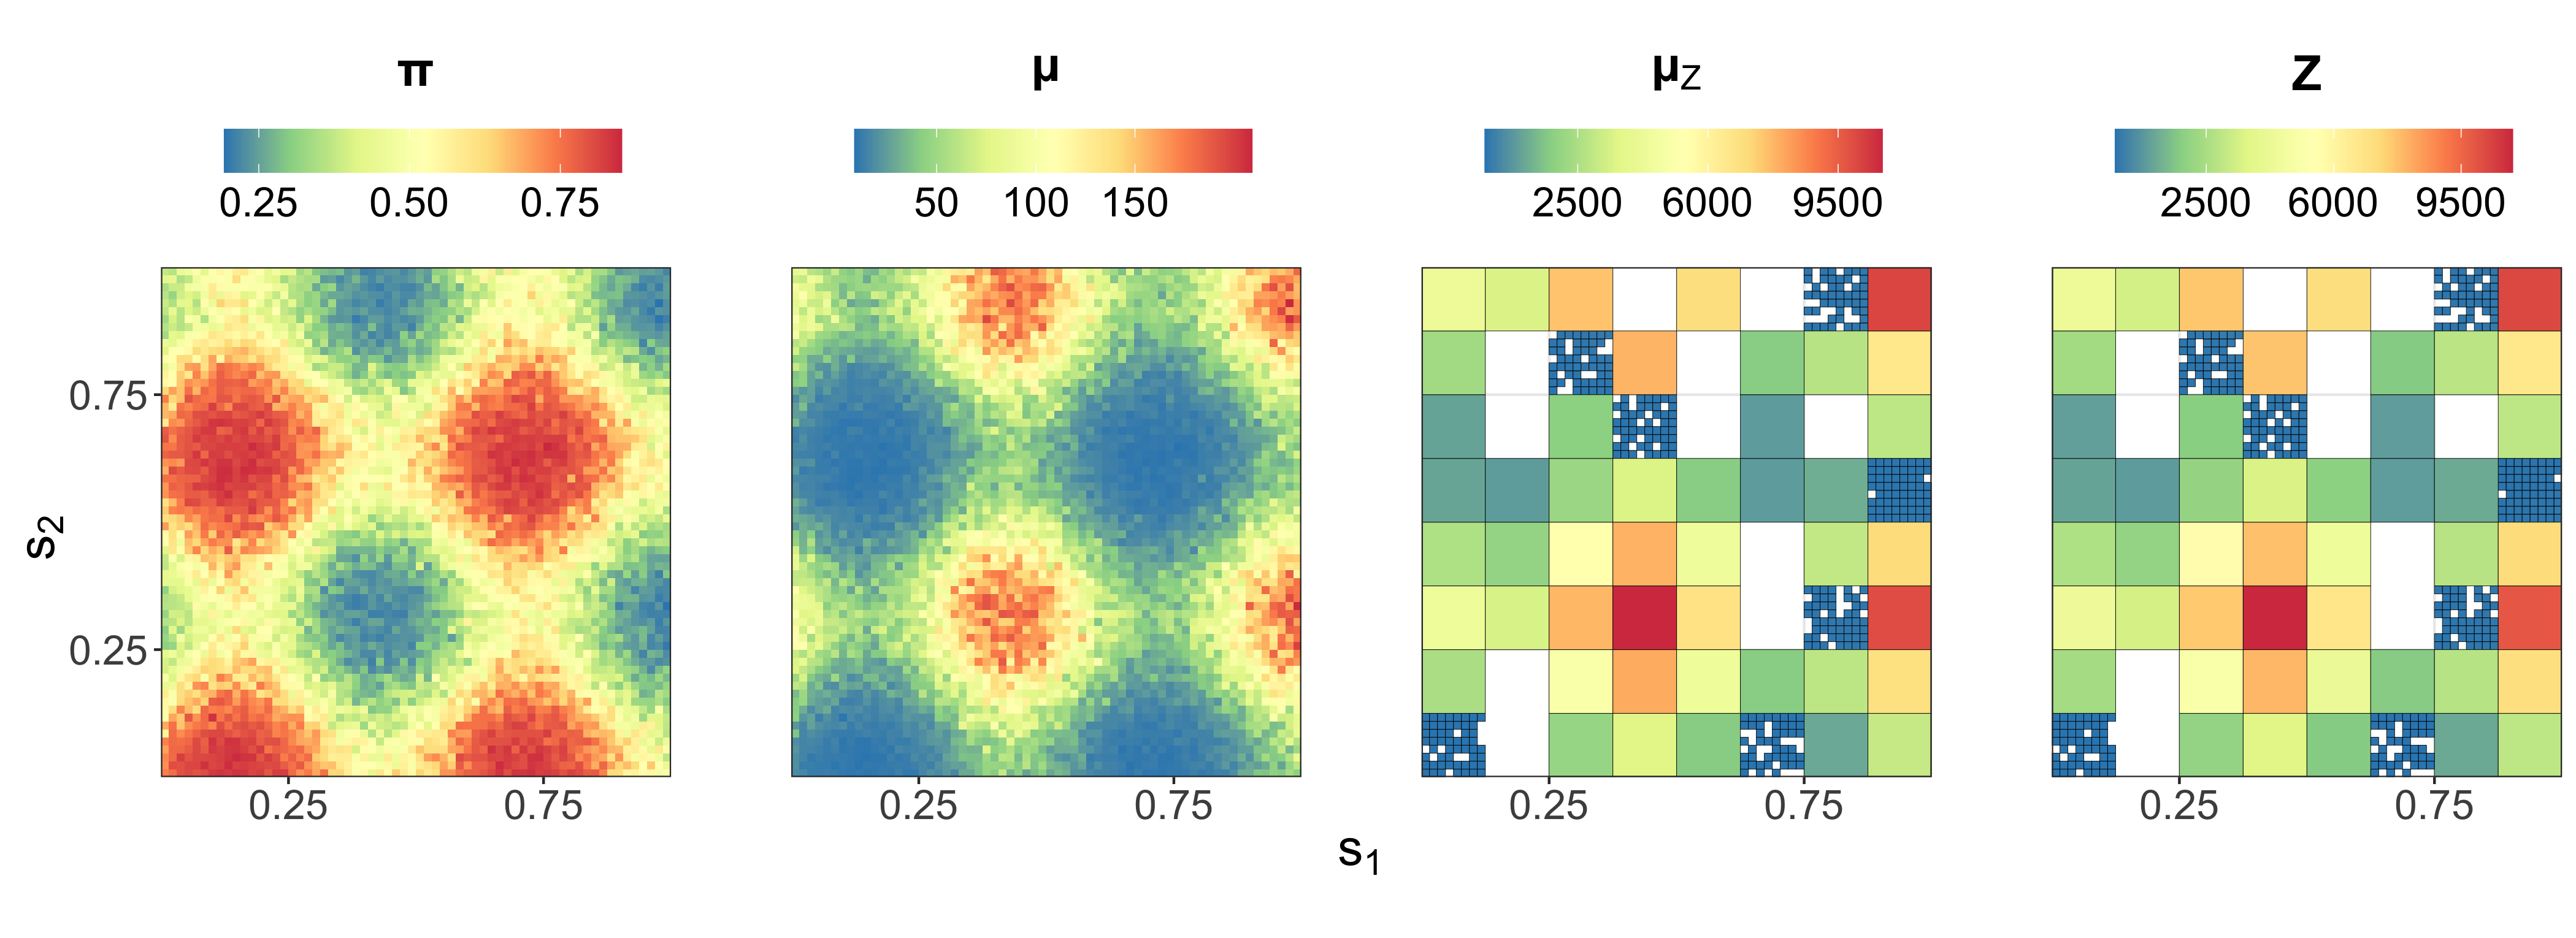
\includegraphics[width = \linewidth]{img/Negbinom_sim_data.png}
    \caption{Simulated, areal negative-binomial data set used in the illustrative example of Section \ref{sec:03-03:negative-binomial}. 
%    (Left panel) Observation and BAU supports. 
    (Left panel) True probability process evaluated over the BAUs. 
    (Centre-left panel) True mean process evaluated over the BAUs. 
    (Centre-right panel) True mean process aggregated to the data support level. 
    (Right panel) Simulated data at the data support level, with some observations omitted; this is the data used for model fitting.  
}   
  \label{fig:03-02-negative-binomial_data}
\end{figure}



%We again use \fct{auto\_basis} to automatically construct the basis functions, and use a scalar  variance matrix for the fine-scale random effects, indicated by setting the \code{fs} field of the BAUs object to one. 
%When the observations are areal, or when we are predicting over large polygons, we must aggregate the mean process over the BAUs (see Section \ref{subsection:04-02:DataLayer}).
%One may cater for unequally weighted BAUs by specifying the weights in the \code{wts} field of the BAU object. 
%In this example, the BAUs are equally sized and are assumed to be of equal weight, so the \code{wts} field is left empty, in which case \pkg{FRK} assumes equally weighted BAUs.





Now we construct and fit the \class{SRE} object using \fct{FRK}. 
 By setting \code{normalise\_wts = FALSE}, we indicate that the weights of $\vec{C}_Z$ and $\vec{C}_P$ should not be normalised, so that the aggregation of the mean process from the BAU level to the data support level corresponds to a sum. 
%When we have areal observations, or when we are predicting over polygons which comprise multiple BAUs, one should declare whether the mean process is to be averaged or summed (see Section \ref{subsection:04-01:ProcessLayer}). 
%In many non-Gaussian applications, it is natural to sum the mean process over the BAUs; this instruction is given by setting \code{normalise\_wts = FALSE}. 
 For binomial and negative-binomial data, the size parameter must be provided: In general, we need the size parameter of every observed BAU. When each observation is associated with exactly one BAU (e.g., point-referenced data, or areal data where the BAUs and observation supports coincide), the user can provide the size parameter with the observations; when some observations are associated with multiple BAUs, the user must provide the size parameter at the BAU level (for all observed BAUs). 
%The size parameter at the BAU level is specified using the field \code{k\_BAU} within the BAU object.
% Here, we also use a scalar fine-scale variance matrix by setting the field \code{fs} of the BAUs object to 1 (implicit in the previous example).
\begin{Code}
R> BAUs$k_BAU <- 50 
R> S <- FRK(f = Z ~ 1, data = list(zdf), BAUs = BAUs, 
+    response = "negative-binomial", link = "logit", normalise_wts = FALSE)
\end{Code}


Next, we predict over the BAUs. 
\begin{Code}
R> pred <- predict(S)
\end{Code}

\begin{figure}[t!]
    \centering
    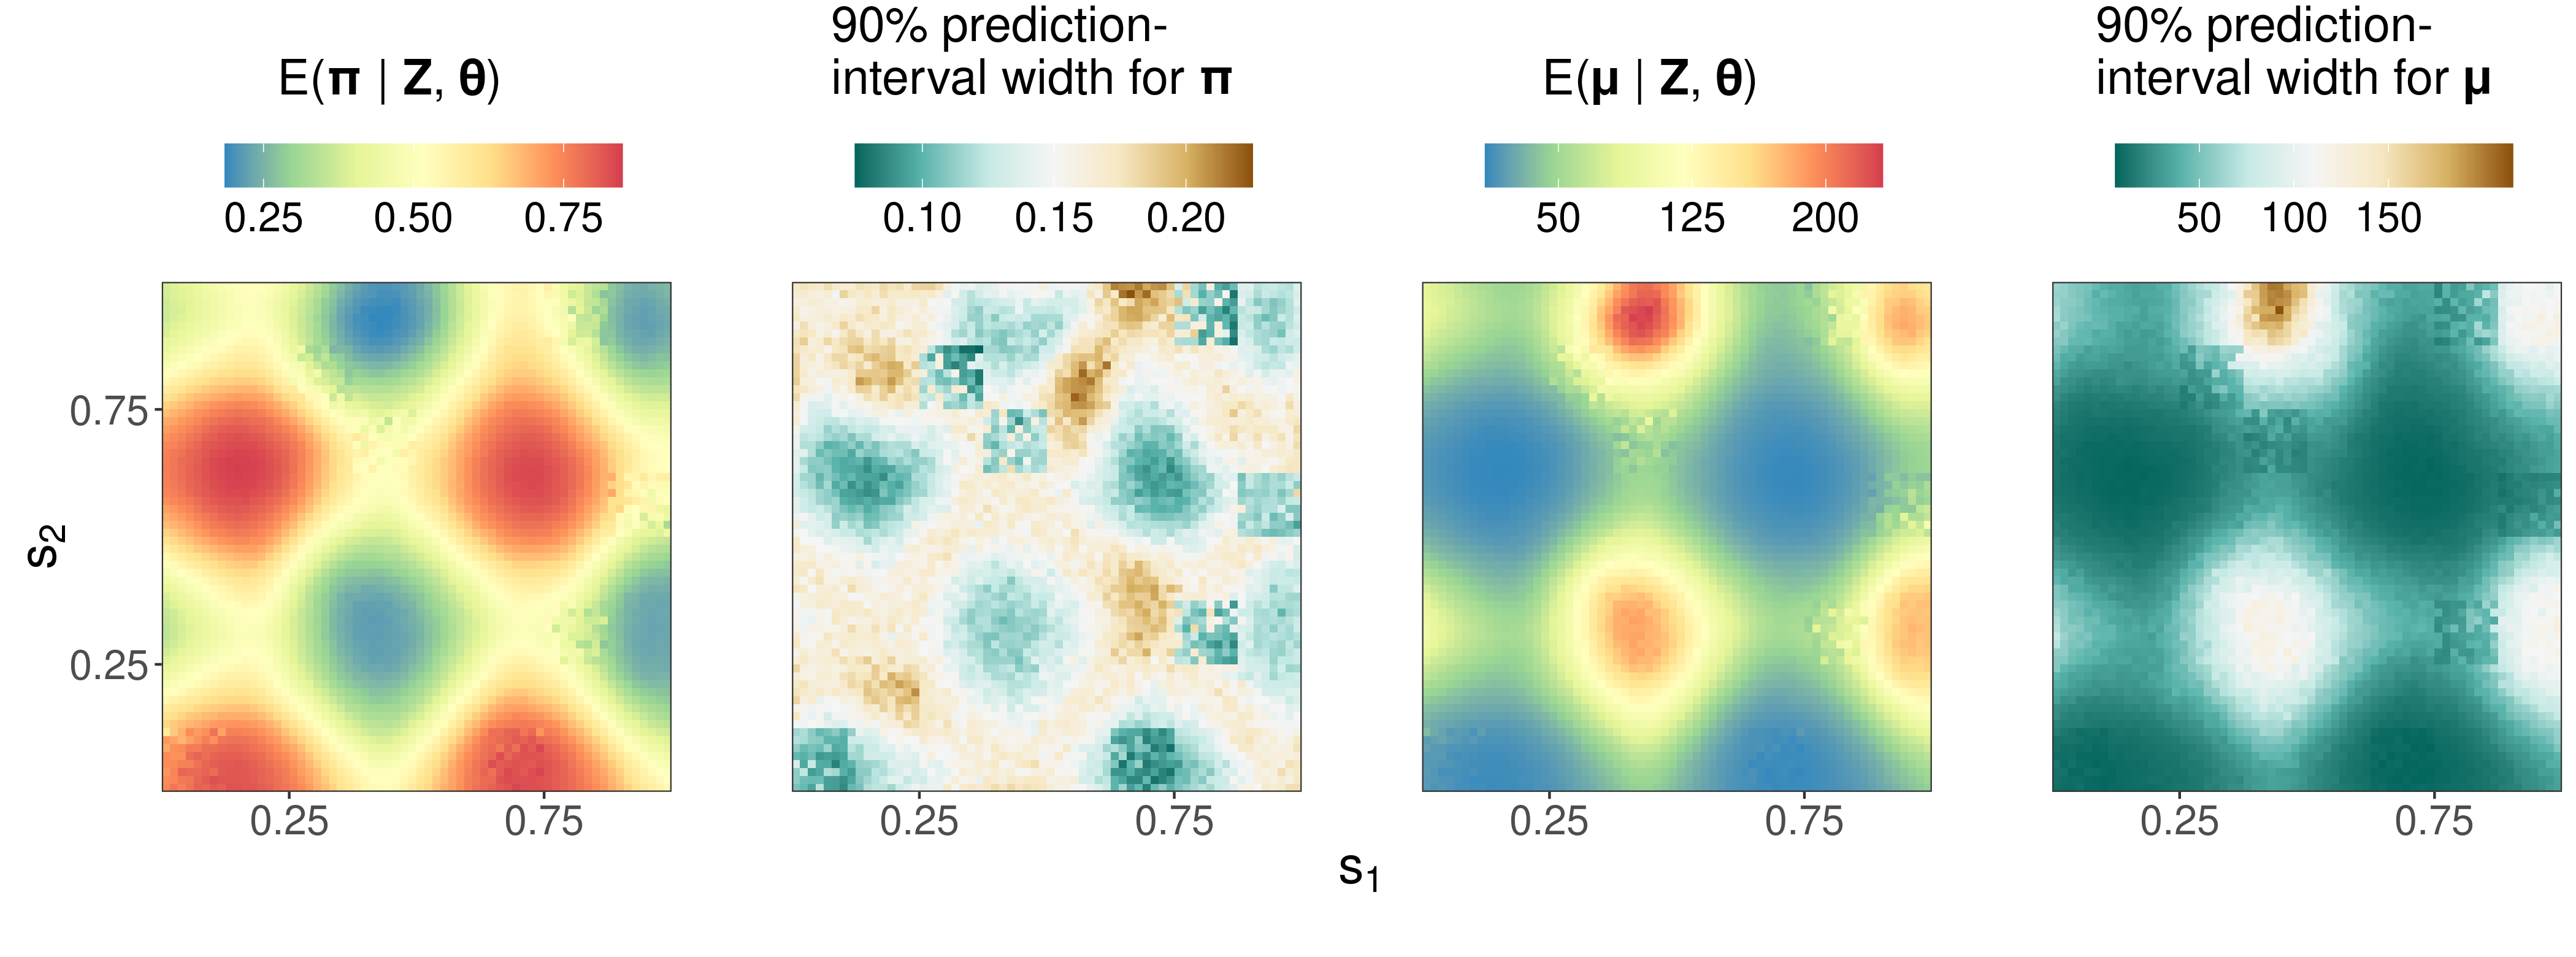
\includegraphics[width = \linewidth]{img/Negbinom_sim_BAU_predictions.png}
    \caption{Prediction and uncertainty quantification of the predictions for the simulated negative-binomial areal example. (Left panel) Prediction of the probability process $\pi(\cdot)$. (Centre-left panel) Width of the 90\% central predictive interval of the probability process. (Centre-right panel) Prediction of the mean process, $\mu(\cdot)$. (Right panel) Width of the 90\% central predictive interval of the mean process.
}   
  \label{fig:03-02-negative-binomial}
\end{figure}

Figure \ref{fig:03-02-negative-binomial} shows the predictions and uncertainty quantification of the predictions  for both the mean process, $\mu(\cdot)$, and the probability process, $\pi(\cdot)$, at the BAU level. 
We observe agreement between the fields shown in Figure \ref{fig:03-02-negative-binomial_data} and the corresponding predictions.  
The prediction uncertainty of $\mu(\cdot)$ is roughly proportional to its prediction. 
In contrast, the prediction uncertainty of $\pi(\cdot)$ is low when the prediction is near 0 or 1, and increases when the prediction is near 0.5: This is expected from properties of the negative-binomial distribution. 
 Uncertainty in both quantities is lower over areas in which we have fine-scale data. 
 The mean empirical coverage from the 90\% posterior predictive intervals was 90.9\%, which is almost nominal, and very reasonable given the difficulty inherent to spatial change-of-support problems.

To emphasise that the prediction polygons are unrelated to the BAUs and data supports, we demonstrate prediction over a handful of irregularly-shaped areas (defined as a \class{SpatialPolygons*} object).  
\begin{Code}
R> pred <- predict(S, newdata = arbitrary_polygons)
\end{Code}
Recall from Section \ref{subsection:04-03:Prediction} that we restrict prediction to $\mu(\cdot)$ over arbitrary polygons.
%; in particular, we do not aggregate the probability process over the polygons. 
Figure \ref{fig:03-02-negative-binomial_polygons} shows the predictions and uncertainty quantification of the predictions over the irregularly-shaped areas. 

\begin{figure}[t!]
    \centering
    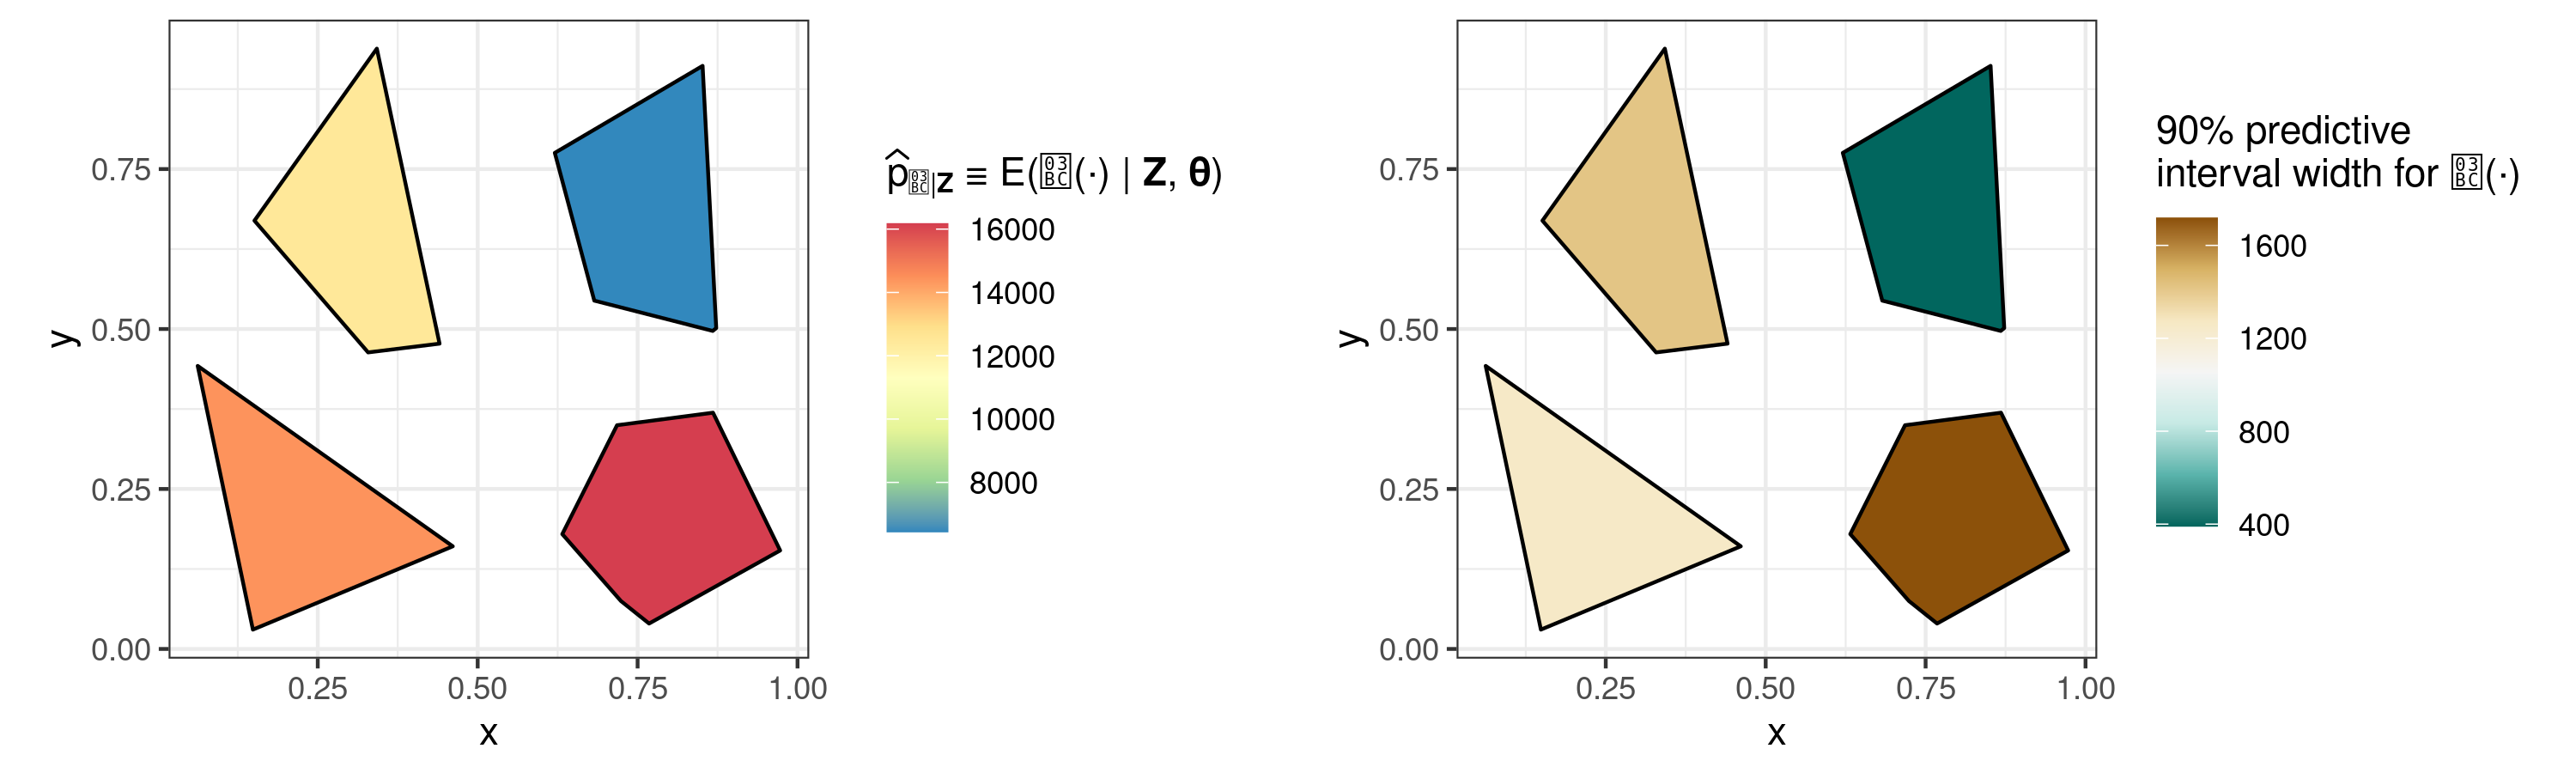
\includegraphics[width = \linewidth]{img/Negbinom_sim_arbitrary_polygon_predictions.png}
    \caption{Prediction (left panel) and prediction uncertainty (right) of the mean process, $\mu(\cdot)$, when predicting over arbitrary polygons in the toy example of Section \ref{sec:03-03:negative-binomial}. Note that these polygons have equal area.}   
  \label{fig:03-02-negative-binomial_polygons}
\end{figure}




%\subsection{Spatial change of support and spatio-temporal extensions}\label{sec:spatial_COS_and_ST}
%
%\pkg{FRK} v2 also caters for spatial areally-referenced data, and spatio-temporal point- and areally-referenced data. For the sake of brevity, we will not use a simple example to show this, and instead refer readers to the application studies presented in Section \ref{sec:spatialCOS} and Section \ref{sec:ST_example}.
% See also the \pkg{FRK} v2 vignette for an example using areal negative-binomial data that demonstrates spatial change of support and prediction over arbitrary, user-defined polygons. 


\subsection{Spatio-temporal extensions}\label{sec:03:Additonal_features}

\pkg{FRK} v2 now also caters for non-Gaussian, point- and areally-referenced, \textit{spatio-temporal} data. 
For the sake of brevity, we will not use a simple example to show this, and instead refer readers to the application study of Section \ref{sec:ST_example}. 
% Examples are given in Section \ref{SEC:ApplicationStudy}.  
% Recall that, when in a spatio-temporal setting, \pkg{FRK} v2 is now able to take advantage of information across time to cater for a spatialy varying fine-scale variance; this is achieved by attributing a separate fine-scale variance parameter to each spatial BAU, and flagged via the \code{fs\_by\_spatial\_BAU} argument (see Section \ref{sec:spatio-temporal} for further details).




\subsection{Support for increased number of basis functions}\label{sec:3:increased_resolution}

The efficiency of \pkg{TMB} and our use of sparse precision matrices means that \pkg{FRK} v2 is now better equipped than \pkg{FRK} v1 to use a large number of basis functions. 
The predictive performance of the framework can be closely related to the number of basis functions, as shown in the following examples. 
Appendix \ref{app:ScoringRules} defines the scoring rules used throughout the remainder of this paper. 



We repeated the analysis in Section \ref{sec:03-01:Poisson} using one, two, and three resolutions of basis functions; Table \ref{tab:03-02:PoissonScoringRules} shows the results for each run. 
%The models' ability to recreate the true process clearly improves as the number of basis function resolutions increases, with an increased number of basis functions consistently leading to lower prediction standard error.
Clearly predictive performance improves as the number of basis functions increases. However, the coverage remains accurate in all runs, implying that the model is able to accurately quantify uncertainty irrespective of the number of basis functions. 
 This important property is in large part due to the fine-scale random variation term, $\xi(\cdot)$, in (\ref{eqn:04-01:Y(s)}). 
\begin{table}[t!]
    \centering
    \caption{Diagnostics comparing the predictive performance when using a range of basis function resolutions and with point-referenced count data. The diagnostics are the root mean-square prediction error (RMPSE), the continuous ranked probability score (CRPS), and the empirical coverage (Cvg90) and interval score (IS90) resulting from a central prediction interval with a nominal coverage of 90\%. The diagnostics are in regards to prediction of the true mean process, $\mu(\cdot)$, and are averaged over all unobserved locations.
% Note that nres = 4 does not improve diagnostics whatsoever    
    }
    \label{tab:03-02:PoissonScoringRules}
    \begin{tabular}{cccccc}
    \hline
    Resolutions (basis functions) & RMSPE  & CRPS & Cvg90 & IS90 & Run Time (Min.) \\
    \hline
    1 (9)    & 83.15    & 47.63 & 0.896  & 377.26  &  0.067  \\
    2 (90)   & 53.96    & 28.54 & 0.893  & 224.24 &  0.128   \\
    3 (819)  & 47.12    & 24.31 & 0.895  & 182.59 &  0.521 \\
%    4 (7380) & 47.27    & 24.40 & 0.895  & 182.91 &  592.23 \\
    \hline
    \end{tabular}
\end{table}




%Figure \ref{fig:Poisson_multires} shows several panels summarising the analysis of the point-referenced Poisson data set shown in Figure \ref{fig:Poisson_true_and_Z}, using one, two, and three resolutions of basis functions.  
%The models' ability to recreate the true process clearly improves as the number of basis function resolutions increases, with an increased number of basis functions consistently leading to lower prediction standard error.  
%Table \ref{tab:03-02:PoissonScoringRules} contains diagnostic scores comparing the predictive performance with a varying number of basis function resolutions. 
%Critically, although all metrics reflect the fact that predictive performance improves with an increasing number of basis functions, the coverage remains accurate irrespective of the number of basis functions, implying that the model is able to accurately quantify uncertainty irrespective of the number of basis functions used. 

  
%Table \ref{tab:03-02:PoissonScoringRules} summarises analyses of the simulated Poisson data shown in Figure \ref{fig:Poisson_true_and_Z} conducted using \pkg{FRK} v2 with one, two, and three resolutions of basis functions. 
%%The models' ability to recreate the true process clearly improves as the number of basis function resolutions increases, with an increased number of basis functions consistently leading to lower prediction standard error.
%Critically, although all metrics reflect the fact that predictive performance improves with an increasing number of basis functions, the coverage remains accurate irrespective of the number of basis functions, implying that the model is able to accurately quantify uncertainty irrespective of the number of basis functions used. 
%\begin{table}[t!]
%    \centering
%    \caption{Diagnostics comparing the predictive performance when using a range of basis function resolutions and with point-referenced count data. The diagnostics are the root mean-square prediction error (RMPSE), the continuous ranked probability score (CRPS), and the empirical coverage (Cvg90) and interval score (IS90) resulting from a central prediction interval with a nominal coverage of 90\%. The diagnostics are in regards to prediction of the true mean process, $\mu(\cdot)$, and are averaged over all unobserved locations.
%% Note that nres = 4 does not improve diagnostics whatsoever    
%    }
%    \label{tab:03-02:PoissonScoringRules}
%    \begin{tabular}{cccccc}
%    \hline
%    Resolutions (basis functions) & RMSPE  & CRPS & Cvg90 & IS90 & Run Time (Min.) \\
%    \hline
%    1 (9)    & 83.15    & 47.63 & 0.896  & 377.26  &  0.067  \\
%    2 (81)   & 53.96    & 28.54 & 0.893  & 224.24 &  0.128   \\
%    3 (729)  & 47.12    & 24.31 & 0.895  & 182.59 &  0.521 \\
%%    4 (7380) & 47.27    & 24.40 & 0.895  & 182.91 &  592.23 \\
%    \hline
%    \end{tabular}
%\end{table}


\begin{table}[t!]
    \begin{center}
    \setlength{\tabcolsep}{5pt}
    \caption{Numerical scoring for each competing method on the MODIS data, as presented in \cite{Heaton_2019_comparative_study}.}
    \label{tab:Heaton_comparison}
    \begin{tabular}{lcccccrr}
    \hline
    Method & MAE  & RMSPE & CRPS & IS95 & Cvg95 & Run Time (Min.) & Cores Used \\[0pt]
    \hline
    \pkg{FRK} v2 & 1.30  & 1.69 & 0.92  & 8.32 & 0.93 & $72.27^{a}$ & $1^{b}$    \\[0pt]
    \pkg{FRK} v1 & 1.96   & 2.44 & 1.44  & 14.08 & 0.79 & 2.32 & 1\\[0pt]
    Gapfill & 1.33   & 1.86 & 1.17  & 34.78 & 0.36 & 1.39 & 40\\[0pt]
    Lattice Krig & 1.22   & 1.68 & 0.87  & 7.55 & 0.96 & 27.92 & 1\\[0pt]
    LAGP & 1.65   & 2.08 & 1.17  & 10.81 & 0.83 & 2.27 & 40\\[0pt]
    Metakriging  & 2.08 & 2.50  & 1.44 & 10.77 & 0.89 & 2888.52 & 30\\[0pt]
     MRA & 1.33 & 1.85 & 0.94 & 8.00 & 0.92 & 15.61 & 1\\[0pt]
    NNGP Conjugate & 1.21 & 1.64 & 0.85 & 7.57 & 0.95 & 2.06 & 10\\[0pt]
    NNGP Response & 1.24 & 1.68 & 0.87 & 7.50 & 0.94 & 42.85 & 10\\[0pt]
    Partition & 1.41 & 1.80 & 1.02 & 10.49 & 0.86 & 79.98 & 55 \\[0pt]
    Pred. Proc. & 2.05 & 2.52 & 1.85 & 26.24 & 0.75 & 640.48 & 1\\[0pt]
    SPDE & 1.10 & 1.53 & 0.83 & 8.85 & 0.97 & 120.33 & 2\\[0pt]
    Tapering & 1.87 & 2.45 & 1.32 & 10.31 & 0.93 & 133.26 & 1\\[0pt]
    Periodic Embedding & 1.29 & 1.79 & 0.91 & 7.44 & 0.93 & 9.81 & 1\\[0pt]
    \hline
    \end{tabular}
    \end{center}
    \begin{tabnote}
$^{a}$\pkg{FRK} v2 was implemented in a different computing environment than the other models, and so run time is not directly comparable. \pkg{FRK} v2 was implemented using a machine with 16 GB of RAM and an Intel i7-9700 3.00GHz CPU with 8 cores. The other models were implemented using the Becker computing environment (256 GB of RAM and 2 Intel Xeon E5-2680 v4 2.40GHz CPUs with 14 cores each and 2 threads per core - totaling 56 possible threads for use in parallel computing) located at Brigham Young University \citep{Heaton_2019_comparative_study}.

$^{b}$\pkg{TMB} supports the use of multiple cores, but this is not yet implemented in \pkg{FRK} v2. 
\end{tabnote}
\end{table}


Although the primary motivation for \pkg{FRK} v2 is the provision of non-Gaussian data models, the ability to use  a large number of basis functions also leads to better predictions in a Gaussian setting.
We show this through the comparative study provided in \cite{Heaton_2019_comparative_study}.
%The data in this study consists of daytime land surface temperatures as measured by the Terra instrument onboard the MODIS satellite \citep{MODIS_satelitte}, with observations on a $500 \times 300$ grid. 
%The training set consists of 105,569 observations, while the test set consists of 42,740 observations.
The data used in that study was made up of a training and a test set consisting of 105,569 and 42,740 observations, respectively; see \cite{Heaton_2019_comparative_study} for a detailed description of the data.
Table \ref{tab:Heaton_comparison} replicates Table 3 of \cite{Heaton_2019_comparative_study}, with an additional entry corresponding to \pkg{FRK} v2, wherein many more basis functions are used than was practical with \pkg{FRK} v1.
 Specifically, \pkg{FRK} v1 used 485 basis functions, whilst \pkg{FRK} v2. uses 12114.
The results show that the increased number of basis functions significantly improves the diagnostic scores of \pkg{FRK}, and the result are now comparable to those of MRA. 
% \red{Furthermore, the Run Time of \pkg{FRK} v2 compared to \pkg{FRK} v1 has increased by a factor similar to the increase in number of basis functions; given that fixed rank kriging generally has a computational cost of $O(r^3)$ (Andrew: is this right, or is it $O(mr^2)$?), this emphasises the relative improvement in computational efficiency of \pkg{FRK} v2.}  
To achieve these improvements over \pkg{FRK} v1, we only had to specify \code{nres = 4}, \code{K\_type = "precision"} and \code{method = "TMB"} in \fct{auto\_basis}, \fct{SRE}, and \fct{SRE.fit}, respectively; the rest of the \pkg{FRK} v1 code as used in the competition was left unchanged. 




%\subsection{Spatio-temporal extensions}\label{sec:03:Additonal_features}
%
%\pkg{FRK} v2 now also caters for non-Gaussian 
% %spatial and 
% spatio-temporal point- and areally-referenced data. 
%For the sake of brevity, we will not use a simple study to show this, but refer readers to the application study of Section \ref{sec:ST_example}. 
%% Examples are given in Section \ref{SEC:ApplicationStudy}.  
% Recall that, when in a spatio-temporal setting, \pkg{FRK} v2 is now able to take advantage of information across time to cater for a spatialy varying fine-scale variance; this is achieved by attributing a separate fine-scale variance parameter to each spatial BAU, and flagged via the \code{fs\_by\_spatial\_BAU} argument (see Section \ref{sec:spatio-temporal} for further details).
%




\section{Application and comparison studies}\label{SEC:ApplicationStudy}


We now provide several application case studies using \pkg{FRK} v2.
In Section \ref{sec:04-01:MODIS}, we present a comparison study between \pkg{FRK} v2 and other packages which cater for non-Gaussian data models. 
In Section \ref{sec:block_prediction}, we demonstrate block prediction using contaminated soil data, and compare our results to other modelling approaches. 
In Section \ref{sec:spatialCOS}, we use data on poverty figures in Sydney, Australia, to demonstrate the spatial change-of-support functionality of \pkg{FRK} v2 in a non-Gaussian setting.
In Section \ref{sec:ST_example}, we provide a non-Gaussian spatio-temporal example through modelling crime counts in the city of Chicago over the first two decades of the 21st century.



\subsection{Comparative study: MODIS cloud data}\label{sec:04-01:MODIS}


In this section we compare out-of-sample predictions from \pkg{FRK} v2 to those from the \proglang{R} packages \pkg{INLA} \citep{Lindgren_2015_R-INLA},  \pkg{spNNGP} \citep{Finley_2020_spNNGP}, \pkg{spBayes} \citep{Finley_2015_spBayes}, and \pkg{mgcv} \citep{Wood_2017_GAM:R} using a binary data set. 
The data form an image of a cloud taken by the Moderate Resolution Imaging Spectroradiometer (MODIS) instrument aboard the Aqua satellite \citep{MODIS_satelitte}. 
Data collected from the MODIS instrument have been used in several related works; see, for instance, \cite{Sengupta_2016_MODIS} and  \cite{ZammitMangion_2021_Deep_compositional_spatial_model}.
For this comparative study, data pre-processing involved first coarsening the image from over 10 million pixels to a more manageable 33750 pixels, by creating a 150 $\times$ 225 grid and computing the mean value of the response within each grid cell. 
Then, as the data provided by the MODIS instrument is continuous (measuring radiance in units of $\text{W/m}^2/\si{\um}/\text{st}$), we applied a reasonable threshold to obtain a binary version of the data (i.e., cloud, or no-cloud).
%The left panel of Figure \ref{fig:03-04-Modis1} displays the processed image of the cloud.  
%In this study, the objective is to predict whether or not each pixel contains cloud cover.
%To obtain a training- and test-set, we used a missing-at-random (MR) sampling scheme, whereby we randomly selected a sub-sample of 6000 pixels to act as training data, and used the remaining 27750 pixels as validation data.
%The right panel of Figure \ref{fig:03-04-Modis1} displays an example of a training set under this sampling scheme.   


We considered two types of sampling schemes for model testing.
 The first was missing-at-random (MR), whereby we randomly selected a sub-sample of pixels to act as training data.
 Under the MR sampling scheme, we randomly sampled 6000 pixels for training, leaving 27750 pixels for testing. 
 The second sampling scheme, which we refer to as `missing-in-a-block' (MB), involved excluding all pixels within a block for training, and using pixels inside the block for testing. 
 The block is a 30 $\times$ 30 square (900 pixels) in the middle of the spatial domain of interest. 
The training and test sets under the two sampling schemes are shown in Figure \ref{fig:03-04-Modis1}.
\begin{figure}[t!]
    \centering
    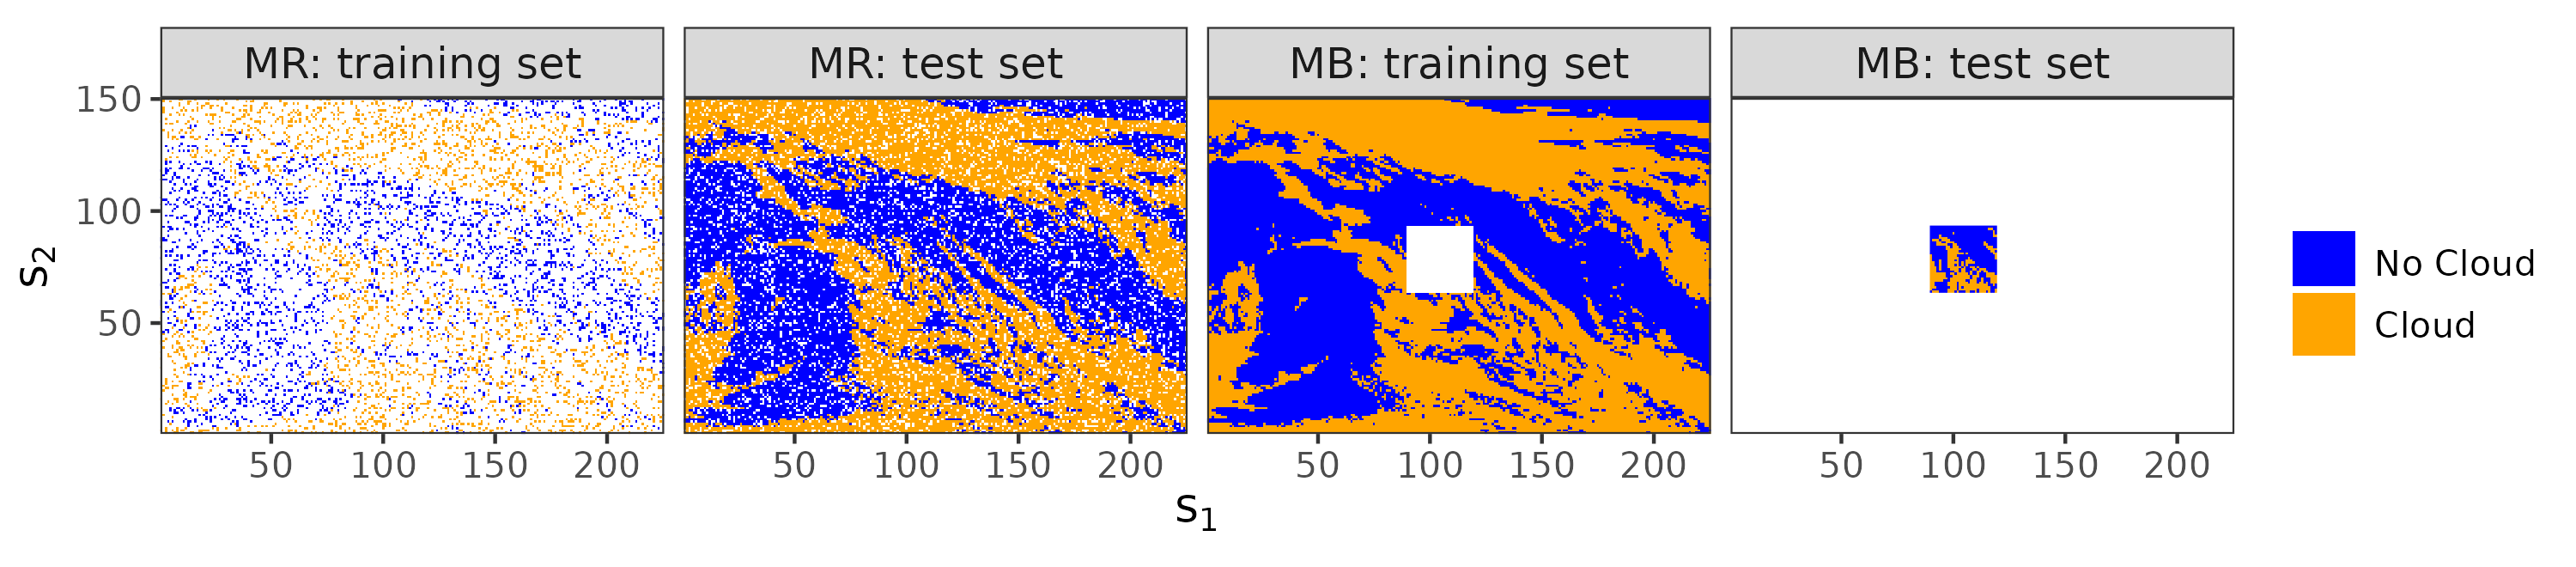
\includegraphics[width = \linewidth]{img/MODIS_data.png}
     \caption{
     MODIS data used in the comparative study of Section \ref{sec:04-01:MODIS}; a blue background is used to make the `No Cloud' and the `Cloud' pixels easier to distinguish. (Left panel) The missing-at-random sample used for training.  (Centre-left panel) The missing-at-random test data. (Centre-right panel) The `missing-in-a-block' sample used for training. (Right panel) The `missing-in-a-block' test data. 
     }\label{fig:03-04-Modis1}
\end{figure}




The software used in this study each required several modelling decisions, which had to be made in a way that balanced predictive performance and run time. 
 We took a systematic approach to a pre-processing model-selection phase by splitting the training set in two, and then using one half for model fitting and the other half for model validation. 
 In this way, we were able to test a large number of arguments for each package, and choose the best combination in terms of predictive performance and run time.  
 For the methods requiring specification of a link function, we used the standard logit link function.
 For \pkg{FRK} v2, we used four resolutions of basis functions; a total of 11,130 basis functions. 
 For \pkg{INLA}, we discretised the domain into 8671 elements.
 We used the \fct{bam} function from \pkg{mgcv}, which is similar to generalised additive model function \fct{gam}, but optimised for large data sets, with 3000 knots. 
For \pkg{spBayes}, we used 400 knots; increasing the number of knots further was computationally prohibitive. 
 We found that the default option of considering 15 neighbours at a time when using \pkg{spNNGP} was appropriate.
 The packages \pkg{spNNGP} and \pkg{spBayes} use Markov chain Monte Carlo (MCMC): At both training and test locations, we used 10000 total MCMC samples, a burn-in of 6000, and a thinning factor of 10; hence, 400 approximately independent samples from the predictive distribution of the process were available at each spatial location. 
The number of cores used for \pkg{spNNGP} can be controlled through the argument \code{n.omp.threads}. 
Setting \code{n.omp.threads} to be greater than 1 did not work on our computing system (a known issue documented in the \pkg{spNNGP} package manual); hence, our reported run-times for \pkg{spNNGP} are for a single core.

 
\begin{figure}
    \centering
    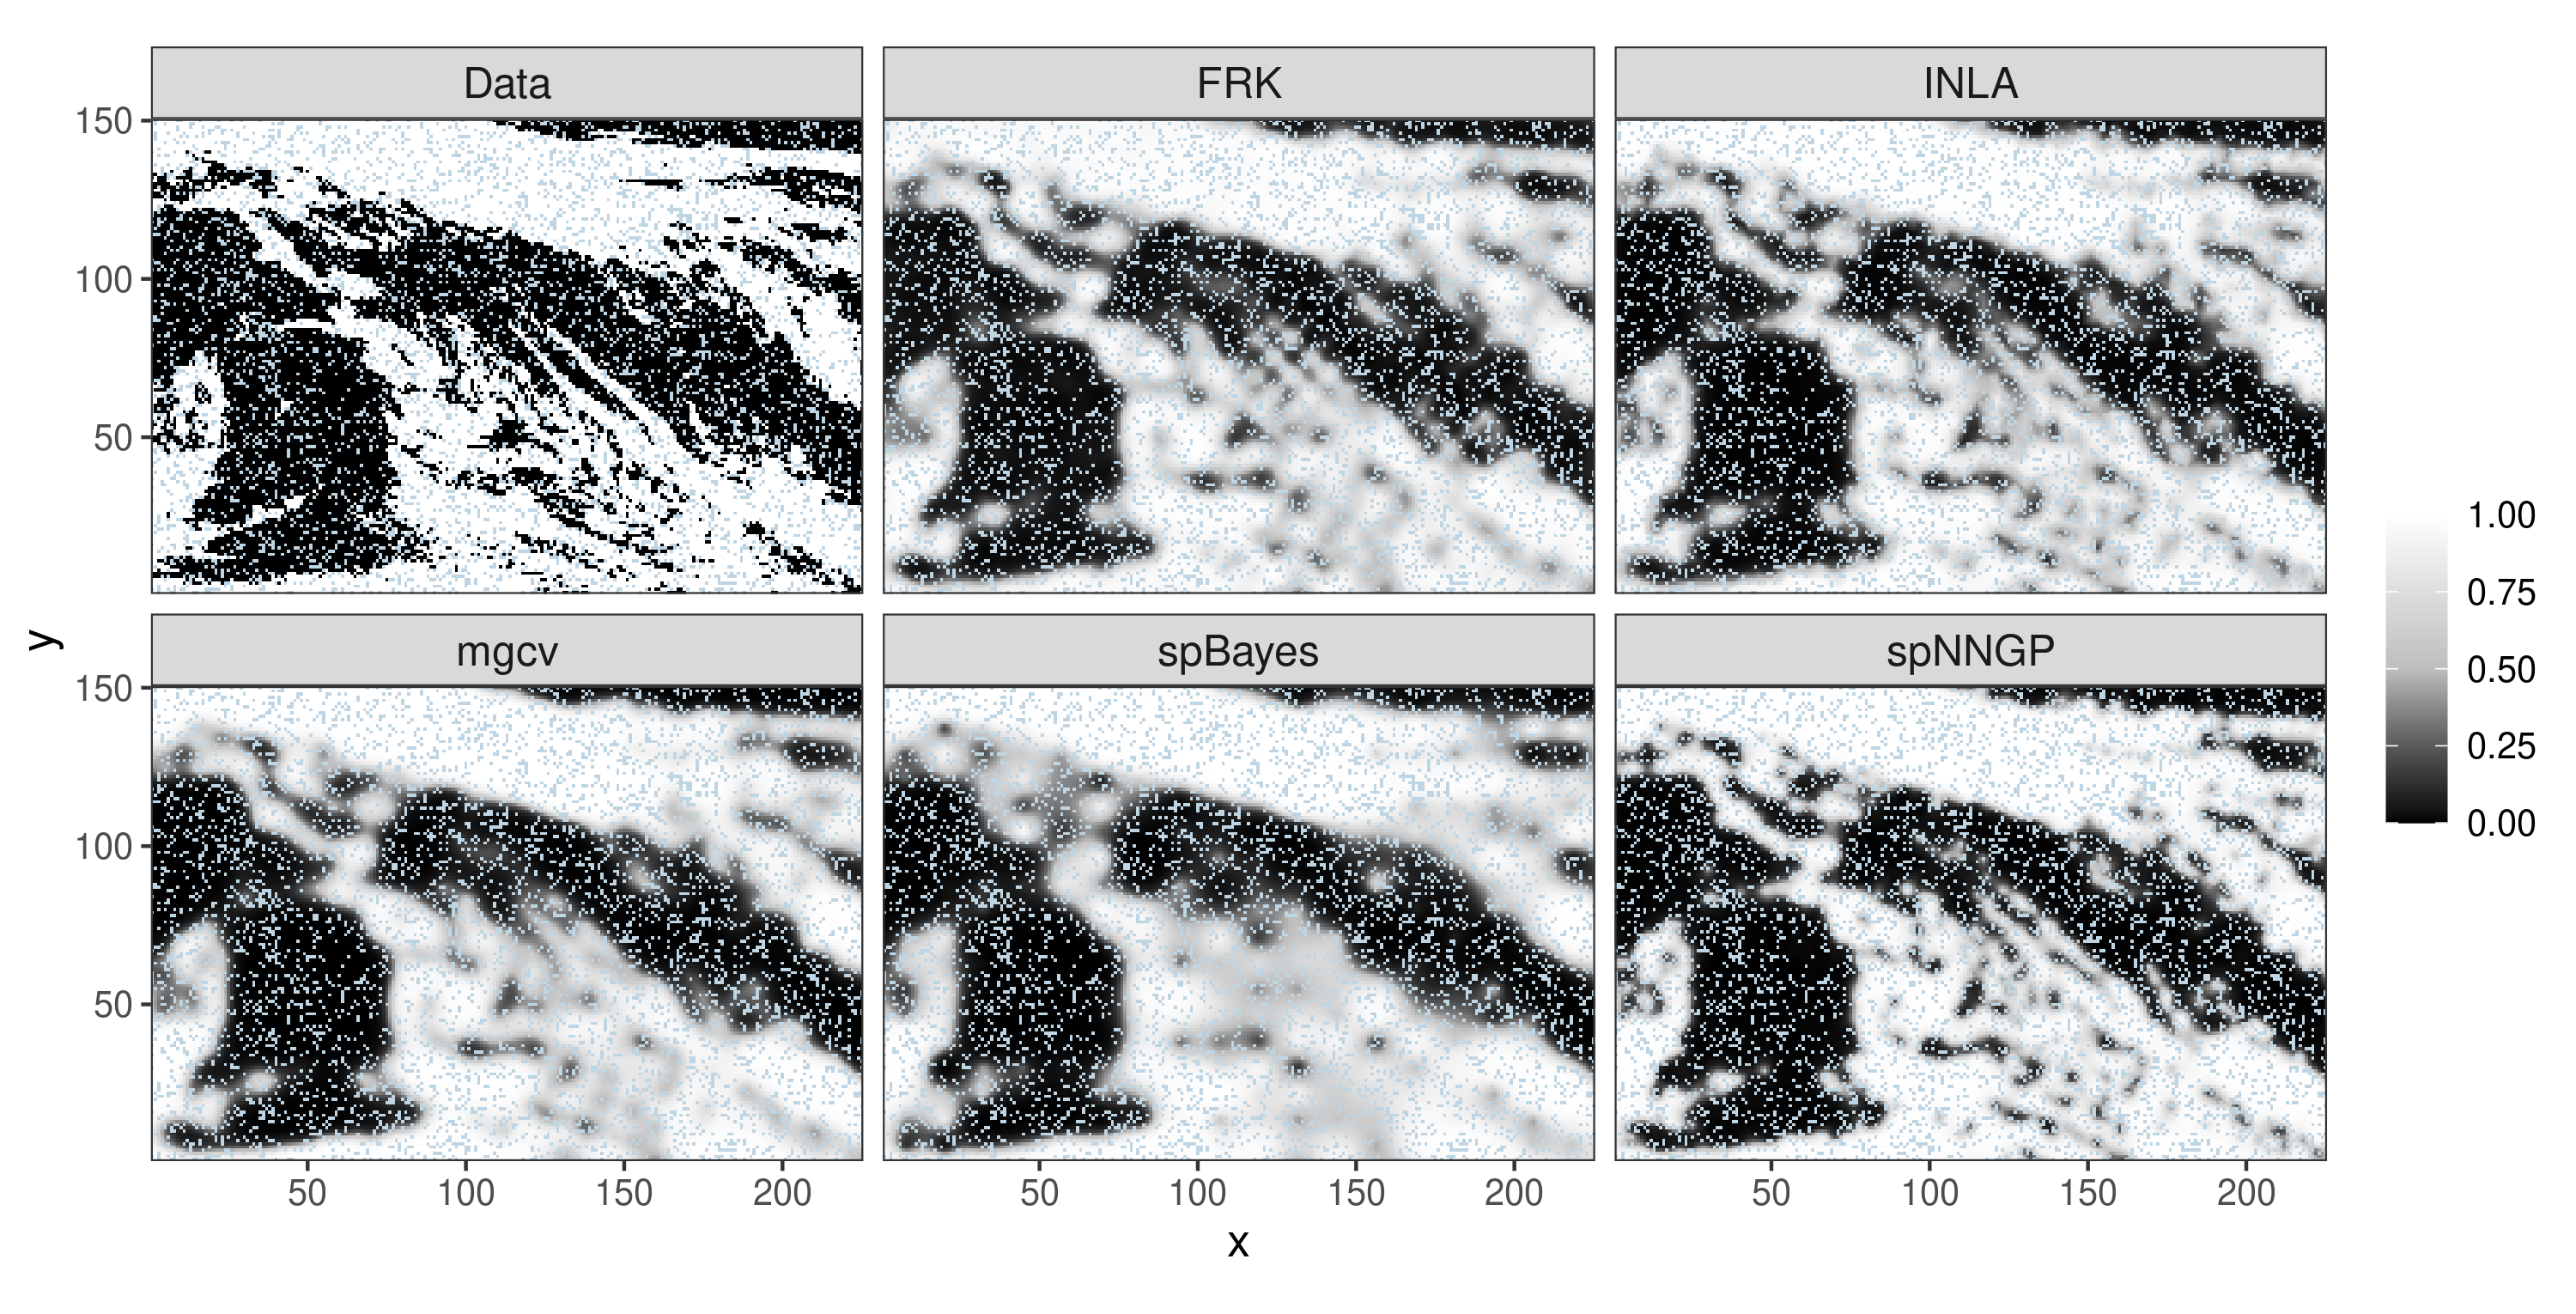
\includegraphics[width = \linewidth]{img/MODIS_MAR_predictions.png}
     \caption{Predictions of the probability of cloud resulting from the missing-at-random data shown in Figure \ref{fig:03-04-Modis1}. Note that the training locations are indicated by blue pixels.}   
  \label{fig:MODIS:pred_MR}
\end{figure}

\begin{figure}[t!]
    \centering
    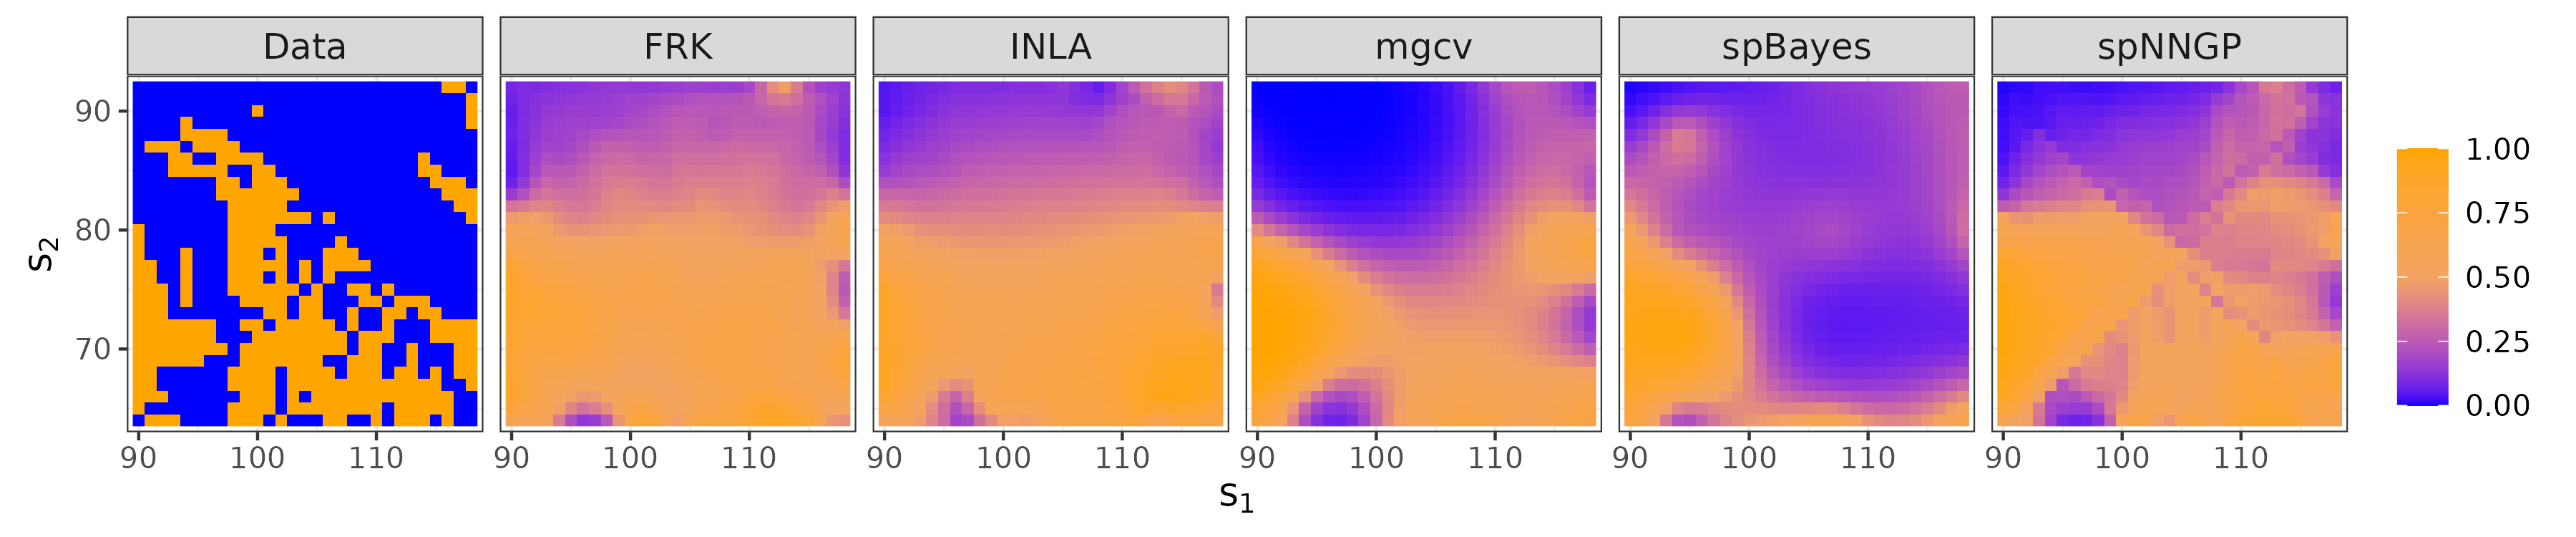
\includegraphics[width = \linewidth]{img/MODIS_block_predictions.png}
     \caption{Predictions of the probability of cloud resulting from the `missing-in-a-block' data shown in Figure \ref{fig:03-04-Modis1}. Here, we have shown only the testing locations, which corresponds to the 30 $\times$ 30 block near the centre of the spatial domain; the test data corresponding to this block is shown in the left-most panel of this figure.}   
  \label{fig:MODIS:pred_block}
\end{figure}










 For each method and each sampling scheme, we predicted the probability of cloud at each pixel. 
 Figure \ref{fig:MODIS:pred_MR} shows the predictions resulting from the MR data shown in Figure \ref{fig:03-04-Modis1}. 
The predictions of \pkg{FRK} v2, \pkg{INLA}, and \pkg{spNNGP} are similar, 
% with the latter appearing to have a slightly sharper resolution, probably because of \pkg{spNNGP}'s use of a nearest-neighbour approach, rather than being based on basis functions. 
 while the predictions of \pkg{mgcv} are slightly smoother than those from the aforementioned packages.
 The predictions of \pkg{spBayes} are even smoother; this is due to the small number of knots. 
 Figure \ref{fig:MODIS:pred_block} shows the predictions resulting from the MB data shown in Figure \ref{fig:03-04-Modis1}. 
 \pkg{FRK} and \pkg{INLA} return predictive probabilities close to 0.5, while \pkg{mgcv} and \pkg{spBayes} are more confident in their predictions. 
 There is an interesting pattern in the \pkg{spNNGP} predictions; this is an expected artefact of the nearest-neighbour approach. 
 
 
 






 
% In a binary setting, the task of assessing prediction uncertainty quantification is difficult, as predictive intervals (based on the probability samples) are in the range $(0, 1)$, and so they will \textit{never} contain the validation data, which take a value in the set $\{0, 1\}$.
The packages used in this study can provide prediction standard errors associated with the probability process. 
However, the underlying distribution of the probability process is unidentifiable, as the posterior predictive distribution, ${Z^*} \mid \vec{Z}$, for some validation datum ${Z^*}$, depends only on the posterior expectation of the probability parameter at the corresponding location, $\ENoLR{\pi^* \mid \vec{Z}}$.
For this reason, we do not attempt to validate the prediction intervals, and instead focus our efforts on predictive accuracy.
\begin{figure}[t!]
    \centering
    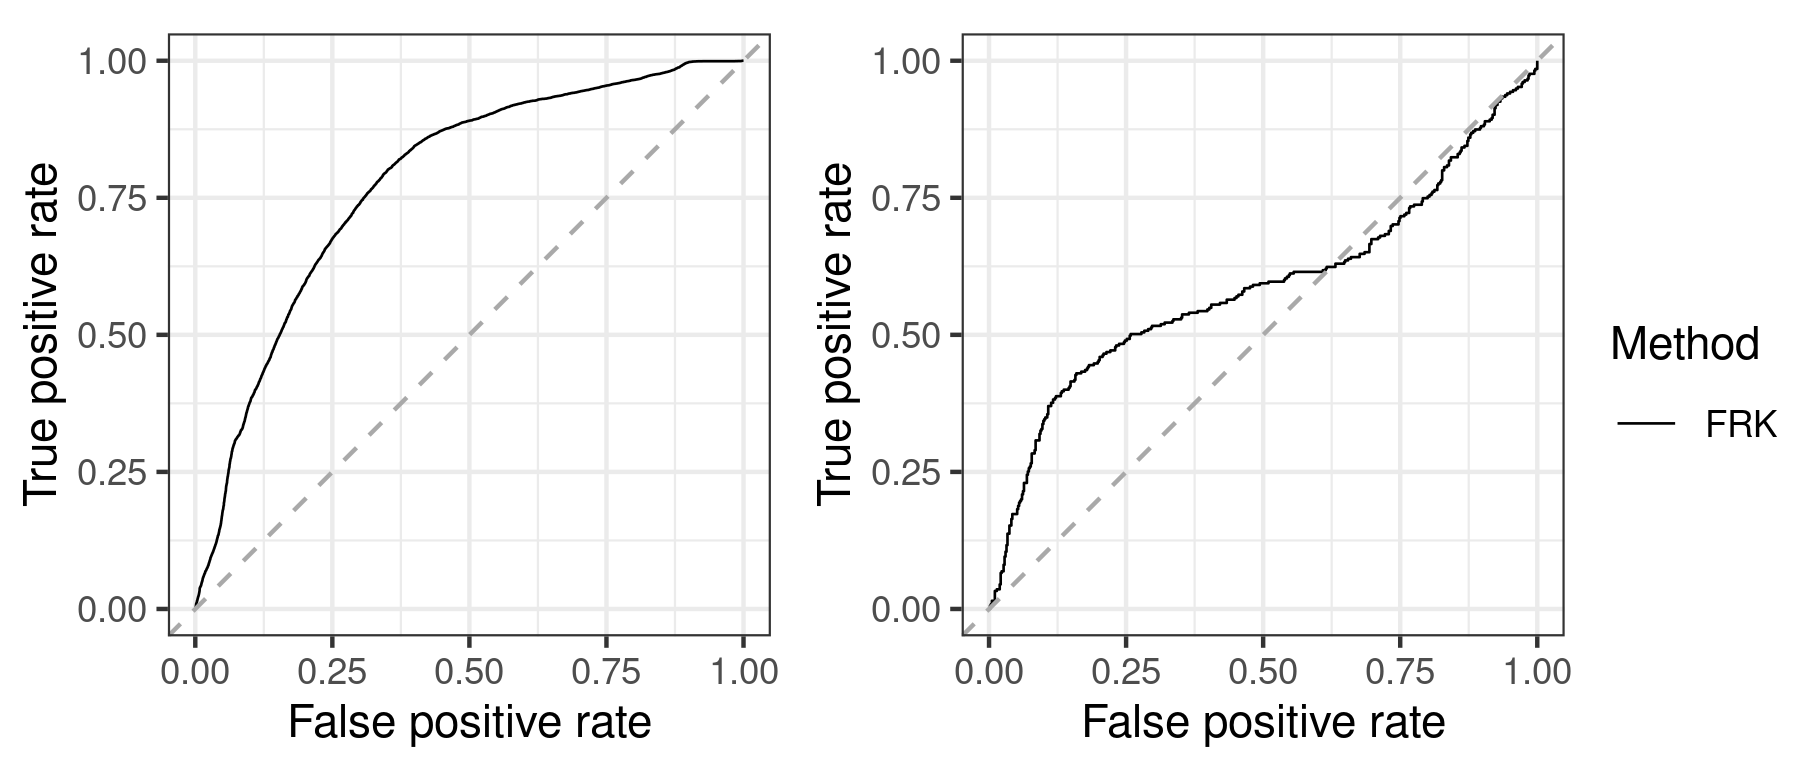
\includegraphics[width = \linewidth]{img/MODIS_ROC.png}
    \caption{ROC curves for the training/test sets displayed in Figure \ref{fig:03-04-Modis1}. (Left panel) ROC curves generated from the `missing-at-random' data. Note that there is some degree of overlap between \pkg{FRK}, \pkg{INLA}, and \pkg{spNNGP}. (Right panel) ROC curves generated from the `missing-in-a-block' data. } 
  \label{fig:MODIS:ROC}
\end{figure}


\begin{table}
    \centering
    \caption{Diagnostic results for the MODIS comparison study. Best performers for a given diagnostic are boldfaced.}
    \label{tab:summary_of_analyses}
    \begin{tabular}{lcccc}
    \hline
   Scheme &  Method  & Brier score & AUC &  Run Time (Min.) \\
   \hline
  MR & FRK & 0.087 & 0.955 & \textbf{5.47} \\ 
   & INLA & 0.090 & 0.951 & 54.44 \\ 
   & mgcv & 0.091 & 0.948 & 45.77 \\ 
   & spBayes & 0.105 & 0.932 & 68.01 \\ 
   & spNNGP & \textbf{0.083} & \textbf{0.956} & 12.35 \\  
   \hline 
MB & FRK & \textbf{0.192} & \textbf{0.769} & \textbf{9.29} \\ 
   & INLA & 0.200 & 0.757 & 141.85 \\ 
   & mgcv & 0.219 & 0.701 & 186.67 \\ 
   & spBayes & 0.247 & 0.632 & 489.41 \\ 
   & spNNGP & 0.198 & 0.749 & 59.30 \\     
   \hline    
  \end{tabular}
\end{table}
 


To assess predictive accuracy, we compared the predictions from all models in terms of the Brier score \citep[Sec.~3]{Gneiting_2007_scoring_rules}, and the area under the receiver operating characteristic (ROC) curve (AUC). %; details of the Brier score are provided in Appendix \ref{app:ScoringRules}. 
The Brier score assesses how close the predicted probability of cloud is to the truth; it is a negatively oriented rule, where low scores indicate accurate predictions of the probability of cloud.
In contrast, higher AUC scores are preferred.
%To obtain reliable estimates of computational times and diagnostic scores, we repeated the experiment with 10 different randomly-sampled training sets, and then averaged the results; these results are reported in Table \ref{tab:summary_of_analyses}. 
The results for each method and each sampling scheme are reported in Table \ref{tab:summary_of_analyses}; the ROC curves are shown in Figure \ref{fig:MODIS:ROC}. 
For the MR scheme, there is little discernible difference between \pkg{FRK}, \pkg{INLA}, \pkg{mgcv}, and \pkg{spNNGP}. 
 However, as one may expect upon viewing the predictions in Figure \ref{fig:MODIS:pred_MR}, \pkg{spBayes} performs poorly in comparison to the other packages due to the small number of knots. 
 The task of prediction over a completely unobserved region is challenging, and so it is no surprise that the diagnostics for the MB scheme are significantly worse than the MR scheme. 
 In this case, we see \pkg{FRK}, \pkg{INLA}, and \pkg{spNNGP} performing slightly better than \pkg{mgcv}, which in turn performs better than \pkg{spBayes}. 
 Note that all run times increased under the MB scheme; however, \pkg{FRK} v2 increased by the smallest amount (increasing by a factor of less than 2), while the run times for other packages increased by between a factor of 3 and 10. 
 Given that the training sample size is significantly larger in the MB scheme than under the MR scheme (32,850 pixels compared to 6000 pixels), this suggests that \pkg{FRK} v2 is well suited to fitting and predicting with large sample sizes.  
 Overall, these results suggest that \pkg{FRK} v2 is comparable to other packages in this application. 
 The advantages of \pkg{FRK} v2 lie in the ease with which it allows one to do other more elaborate analyses with non-Gaussian data, as shown in the next sections. 
 
 














\subsection{Block prediction: Contaminated soil}\label{sec:block_prediction}

%\red{(Not sure how much emphasis must be placed on the merits of \pkg{FRK} over \pkg{georob}, but other points in \pkg{FRK}'s favour are that it can also cater for spatio-temporal data (\pkg{georob} cannot), as well as cater for many more non-Gaussian distributions (\pkg{georob} cannot). There is probably an argument to be made that \pkg{FRK} is more user friendly, but I suppose this is subjective, and probably not appropriate for a package co-author to comment on.)}
%
%
%\red{(The Paul and Cressie plots only go to a block size of about 190, while mine extend to a block size of 250. I manually computed the square root of the area of their largest block (being conservative with the boundaries), and found it to be 245. So, I believe that either (i) the Paul and Cressie plots are cut off at a certain point, (ii) a mistake has been made in computing the block sizes, or (iii) the block sizes are not computed simply by taking the square root of the area. I investigated the third point, and I think I can rule out the thought that they used the diagonal length of the block rather than the area, because I computed the diagonal length (just using Pythagoras' theorem) of the largest block and found it to be around 350.    )}



Between 1954 and 1963, nuclear devices were detonated at Area 13 of the Nevada Test Site in the United States, contaminating the surrounding soil with the radioactive element americium (Am). 
%In 1971, the Nevada Applied Ecology Group measured Am concentrations in a region surrounding Ground Zero (GZ), the location where the devices were detonated \citep{Paul_Cressie_2011_lognormal_kriging_block_prediction}. 
The data we use in this example contains 
%measurements of Eastings (m), Northings (m), and 
 Am concentrations (in $10^3$ counts per minute) in a spatial domain immediately surrounding Ground Zero (GZ), the location where the devices were detonated, and was previously analysed by \cite{Huang_2009_multivar_intrinsic_rand_functions_cokriging} and \cite{Paul_Cressie_2011_lognormal_kriging_block_prediction}. 
%Measurements were recorded at 196 unique locations, but the presence of several colocated measurements bring the total number of observations to 212. 
The total number of measurements (including some that are collocated) is 212.
The left and centre panels of Figure \ref{fig:Am_data} shows the data on the original scale and on the log scale, respectively.
\cite{Paul_Cressie_2011_lognormal_kriging_block_prediction} note that the Am concentrations are clearly lognormally distributed, and that soil remediation is often made by averaging the contaminant over pre-specified spatial regions of $D$ called blocks.
Hence, %soil remediation for 
 this application requires lognormal prediction over blocks, a task well suited to \pkg{FRK} v2. %wherein predictions are easily made over arbitrary user-specified regions. 
% Following \cite{Paul_Cressie_2011_lognormal_kriging_block_prediction}, we use two blocking schemes, one centred on GZ, and the other centred away from GZ; these schemes are shown in right panel of Figure \ref{fig:Am_data}.
 The right panel of Figure \ref{fig:Am_data} shows two blocking schemes which we will predict over: Both schemes contain 5 blocks, but one scheme is centred on GZ, and the other is centred away from GZ.
% Following \cite{Paul_Cressie_2011_lognormal_kriging_block_prediction}, we use two blocking schemes, one centred on GZ, and the other centred away from GZ; these schemes are shown in right panel of Figure \ref{fig:Am_data}. 
% Note that \pkg{FRK} v2 does not explicitly cater for a lognormal response, but an effective approach is to use \code{response = "Gaussian"} and \code{link = "log"}. 
\begin{figure}
    \centering
    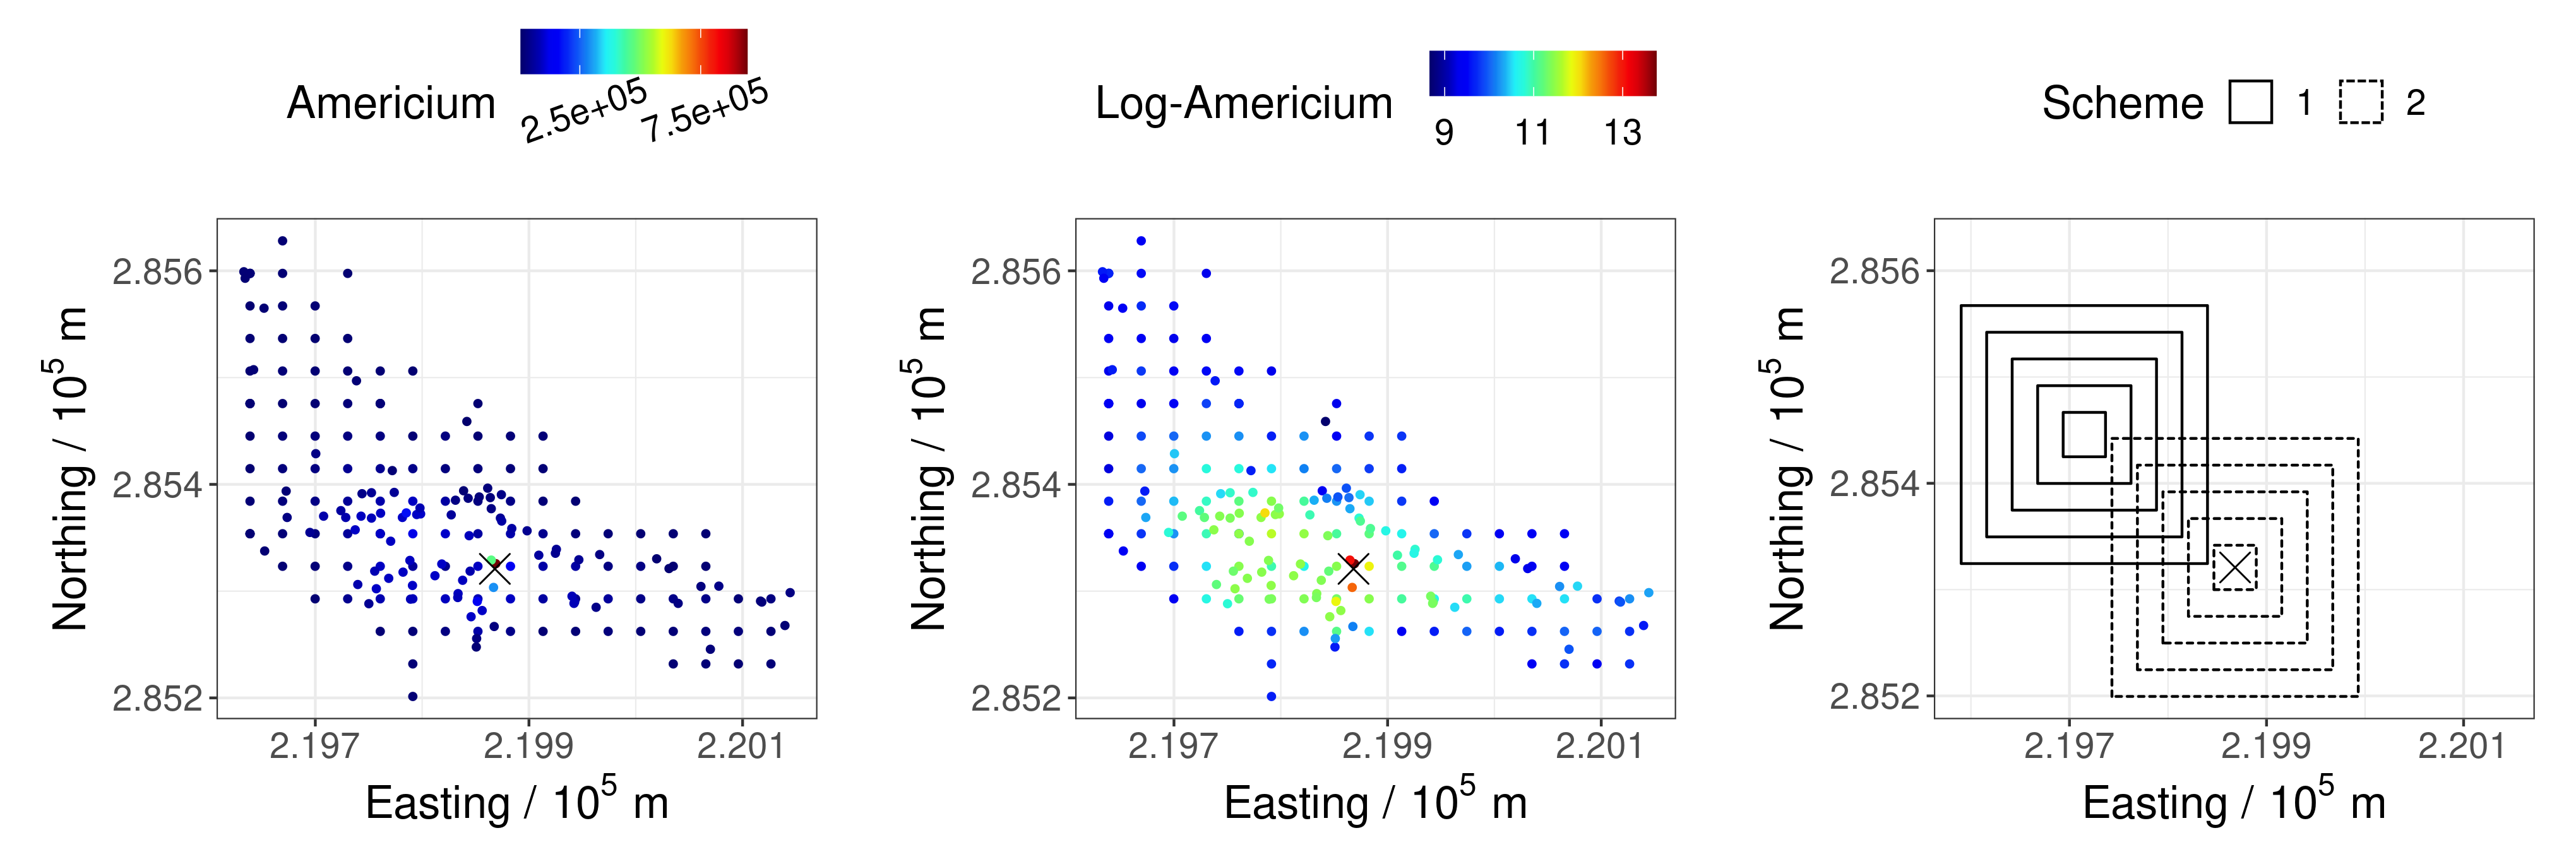
\includegraphics[width = \linewidth]{img/Am_data_and_blocks.png}
    \caption{Americium soil data. The `$\times$' denotes Ground Zero (GZ), where the devices were detonated. (Left panel) Am concentrations on the original scale. (Centre panel) Am concentrations on the log scale. (Right panel) Americium soil data blocking schemes: Scheme 1 (red), centred away from GZ, and Scheme 2 (blue), centred on GZ. 
%    \red{(Andrew: Given that some locations are associated with multiple observations, this figure may be inadequate. I believe this may be why \cite{Paul_Cressie_2011_lognormal_kriging_block_prediction} opted to use a bubble plot.)}
}   
  \label{fig:Am_data}
\end{figure}

%Figure \ref{fig:Am_data} shows that, as one would expect, the Am concentrations decline with increasing distance from GZ. 
%This trend may be accounted for by including distance from GZ as a covariate.
%\cite{Paul_Cressie_2011_lognormal_kriging_block_prediction} observe that the Am concentrations near GZ exhibit a different spatial variation from those in the rest of the region; hence instead of fitting a single linear trend, they fit two separate regression lines, one using only the observations that are within a distance of 30.48m from GZ, and the other using the remaining observations.
%We will do the same; 
As in \cite{Paul_Cressie_2011_lognormal_kriging_block_prediction}, we use a piecewise linear trend, where observations within a distance of 30.48m from GZ follow a different trend to those observations beyond 30.48m from GZ. %;
%denoting the Euclidean distance between GZ and location $\vec{s}$ by $d(\vec{s})$, the covariates used in our model are
%\[
%\vec{t}(\vec{s})
%=
%[I(d(\vec{s}) < 30.48),\, d(\vec{s})I(d(\vec{s}) < 30.48),\, I(d(\vec{s}) \geq 30.48),\, d(\vec{s})I(d(\vec{s}) \geq 30.48)]^\tp.
%\]
The following code constructs the required BAU level covariates. %there are four covariates required to construct a piecewise temporal trend, and we name these as \pkg{x1} through to \pkg{x4}. 
\begin{Code}
R> d_BAU   <- distR(coordinates(BAUs), Ground_Zero)
R> BAUs$x1 <- d_BAU * (d_BAU < 30.48)
R> BAUs$x2 <- d_BAU >= 30.48
R> BAUs$x3 <- d_BAU * (d_BAU >= 30.48)
\end{Code}
Modelling for this problem is done by setting \code{response = "Gaussian"} and \code{link = "log"}. 
 In order to mimic lognormal block kriging, here we fix the measurement error standard deviation to a  small value prior to model fitting. 
%\red{Note that we omit an overall mean from the covariates, as this overall mean is confounded with the intercepts. Andrew: actually, we can include an overall mean, and then omit one of the intercepts.}
\begin{Code}
R> Am_data$std <- 1 
R> S <- FRK(f = Am ~ x1 + x2 + x3, data = list(Am_data), BAUs = BAUs,
+    response = "gaussian", link = "log", est_error = FALSE) 
\end{Code}

\begin{figure}
    \centering
    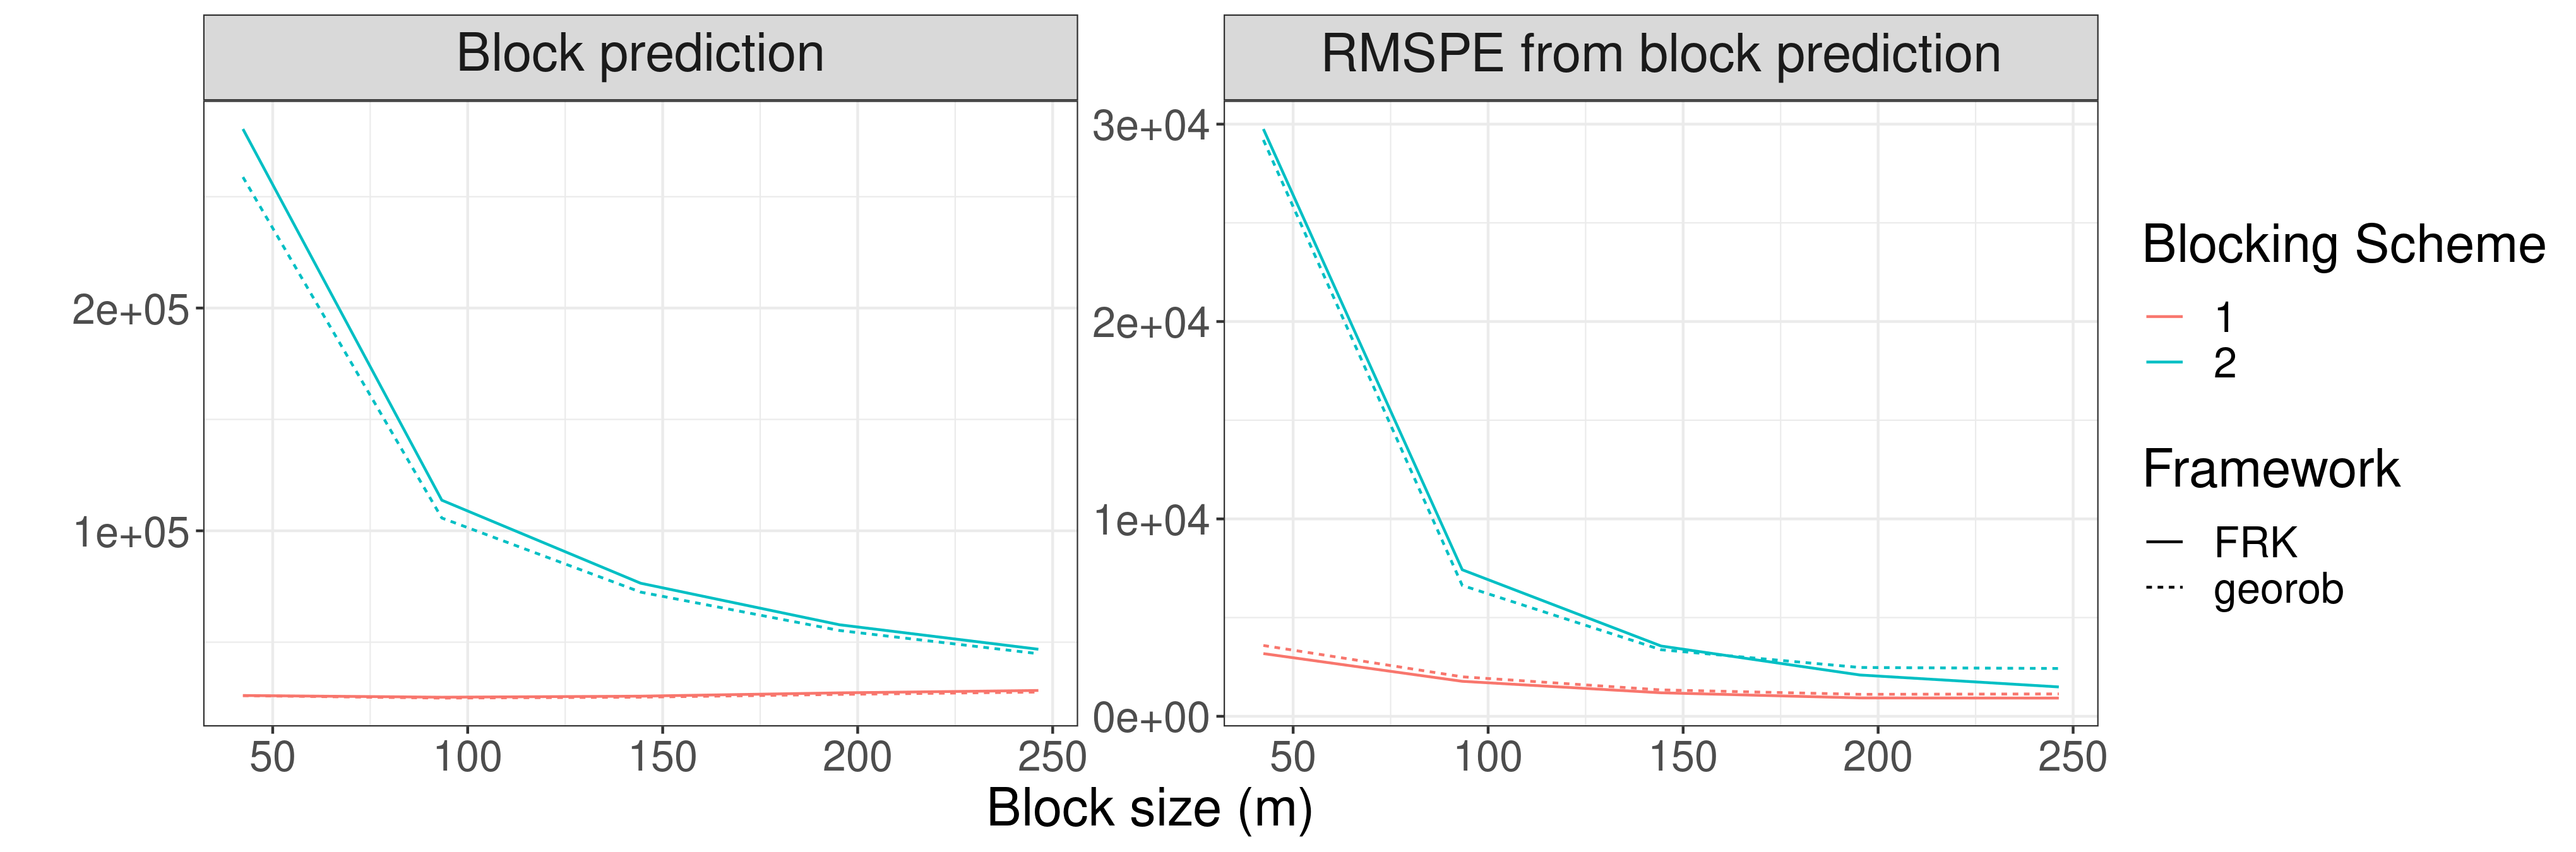
\includegraphics[width = \linewidth]{img/Am_comparison.png}
    \caption{Predictions and root mean squared prediction error (RMSPE) against block size for the two blocking schemes. (Left panel) Block-predictions of Am concentrations against block size $|B|^{1/2}$.  (Right panel) RMSPE of block predictions of Am concentrations against block size $|B|^{1/2}$. In both plots, the red line corresponds to Scheme 1 and the blue line corresponds to Scheme 2.
}   
  \label{fig:Americium_block_preds_by_size}
\end{figure} 


By predicting over the BAUs, one may generate predictions over the entire spatial domain. %as depicted in Figure \ref{fig:Am_BAU_predictions}.
Alternatively, by passing a \class{SpatialPolygonsDataFrame} object into the \code{newdata} argument of \fct{predict}, one may straightforwardly generate block-level predictions.
% \citet*[ch.~3]{Cressie_1993_stats_for_spatial_data}
% \cite[][App.~C]{Cressie_2006_block_kriging_lognormal_spatial_processes}




%Another \proglang{R} package thats performs lognormal block predictions is \pkg{georob} \citep{georob}, which, using methods proposed by \cite{Cressie_2006_block_kriging_lognormal_spatial_processes}, implements an approximately unbiased back-transformation of kriging predictions of log-transformed data.
To compare our predictions, we used the \proglang{R} package \pkg{georob} \citep{georob}, which implements an approximately unbiased back-transformation of kriging predictions of log-transformed data \citep{Cressie_2006_block_kriging_lognormal_spatial_processes}. 
Kriging does not scale well for large sample sizes, however %as
 the size of this data set is small. %, \pkg{georob} can be used to validate the predictions and associated uncertainty quantification obtained using \pkg{FRK} v2. 
 The package \pkg{georob} provides users with two approaches to lognormal block kriging; 
%the first assumes permanence-of-lognormality, that is, that both point and block values follow log-normal laws, which cannot strictly hold, whilst the second, referred to as the optimal predictor, involves averaging back-transformed point predictions over the blocks. 
% The assumption of permanence-of-lognormality does not have a significant impact on the back-transformation when the blocks are small \citep{Cressie_2006_block_kriging_lognormal_spatial_processes}, however, for larger blocks, it is recommended to use the so-called optimal predictor. 
we used the `optimal predictor', as recommended by the \pkg{georob} manual when predicting over large blocks.
%as the bias introduced by the assumption of permanence-of-lognormality typically has a greater impact on the back-transformation when the blocks are large \citep{Cressie_2006_block_kriging_lognormal_spatial_processes}. 
%Hence, as the blocking schemes in this application contain relatively large blocks, we will use the optimal predictor.
Figure \ref{fig:Americium_block_preds_by_size} shows the block predictions and associated RMSPE obtained using \pkg{FRK} v2 and \pkg{georob} for the two blocking schemes shown in Figure \ref{fig:Am_data}.
The similarity in results lends confidence that the predictions and associated prediction standard errors obtained using \pkg{FRK} v2 are reasonable.
%, and suggests that, despite the fact that \pkg{FRK} v2 uses low-rank approximations, the results are comparable to those obtained using `exact' methods.
%Figure \ref{fig:Americium_block_preds_by_size} shows that, as one may expect, the block predictions of Scheme 1 (centred away from GZ) are smaller than the block predictions of Scheme 2 (centred on GZ). 
%In Scheme 1, the block predictions gradually increase with block size, as the blocks become closer to GZ; in Scheme 2, we witness the opposite behaviour, with the block predictions dropping rapidly with block size, as the area immediately surrounding GZ becomes an increasingly small percentage of the blocks. 
%In both schemes, the RMSPE decreases with block size, but it is consistently larger in Scheme 2 than in Scheme 1. 
%% The results obtained using \pkg{FRK} v2 and \pkg{georob} do not corroborate those of \cite{Paul_Cressie_2011_lognormal_kriging_block_prediction}.
%Whilst the predictions obtained using \pkg{FRK} v2 and \pkg{georob} are (somewhat) similar to those provided by \cite{Paul_Cressie_2011_lognormal_kriging_block_prediction}, there is a significant discrepancy between the reported RMSPE. In particular, \cite{Paul_Cressie_2011_lognormal_kriging_block_prediction} report a larger RMSPE (by a factor of between 1.5 and 10) for both blocking schemes, and, in Scheme 2, their RMSPE decreases at a slower rate, with the RMSPE decreasing linearly with the block-size.



% \begin{figure}
%     \centering
%     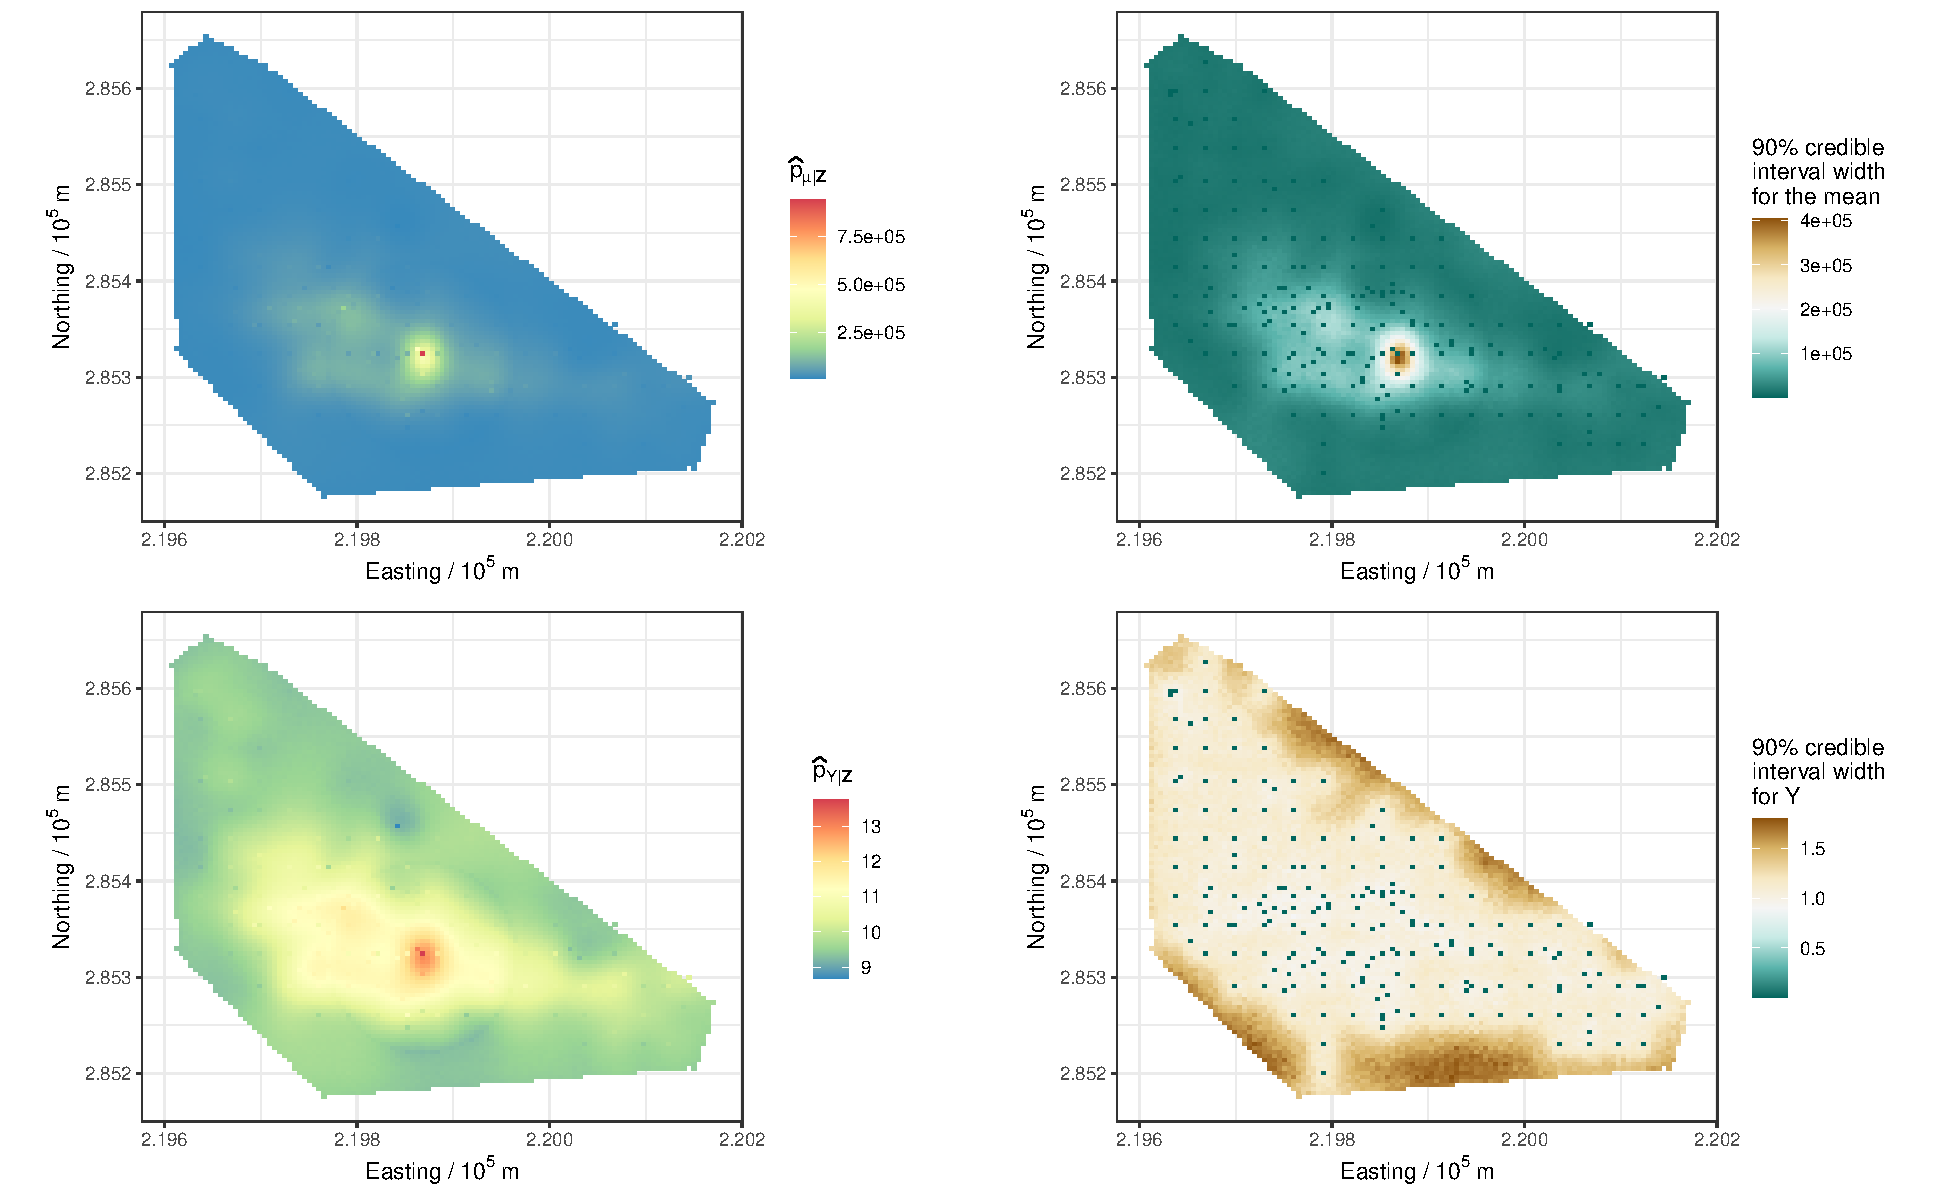
\includegraphics[width = \linewidth]{img/Americium_BAU_predictions.png}
%     \caption{BAU level predictions of the Americium data set. (Top-left panel) Predictions on the data scale. (Top-right panel) Prediction interval on the data scale. 
%     (Bottom-left panel) Predictions on the log scale. (Bottom-right panel) Prediction interval on the log scale.  
% }   
%   \label{fig:Am_BAU_predictions}
% \end{figure}


% \begin{figure}
%     \centering
%     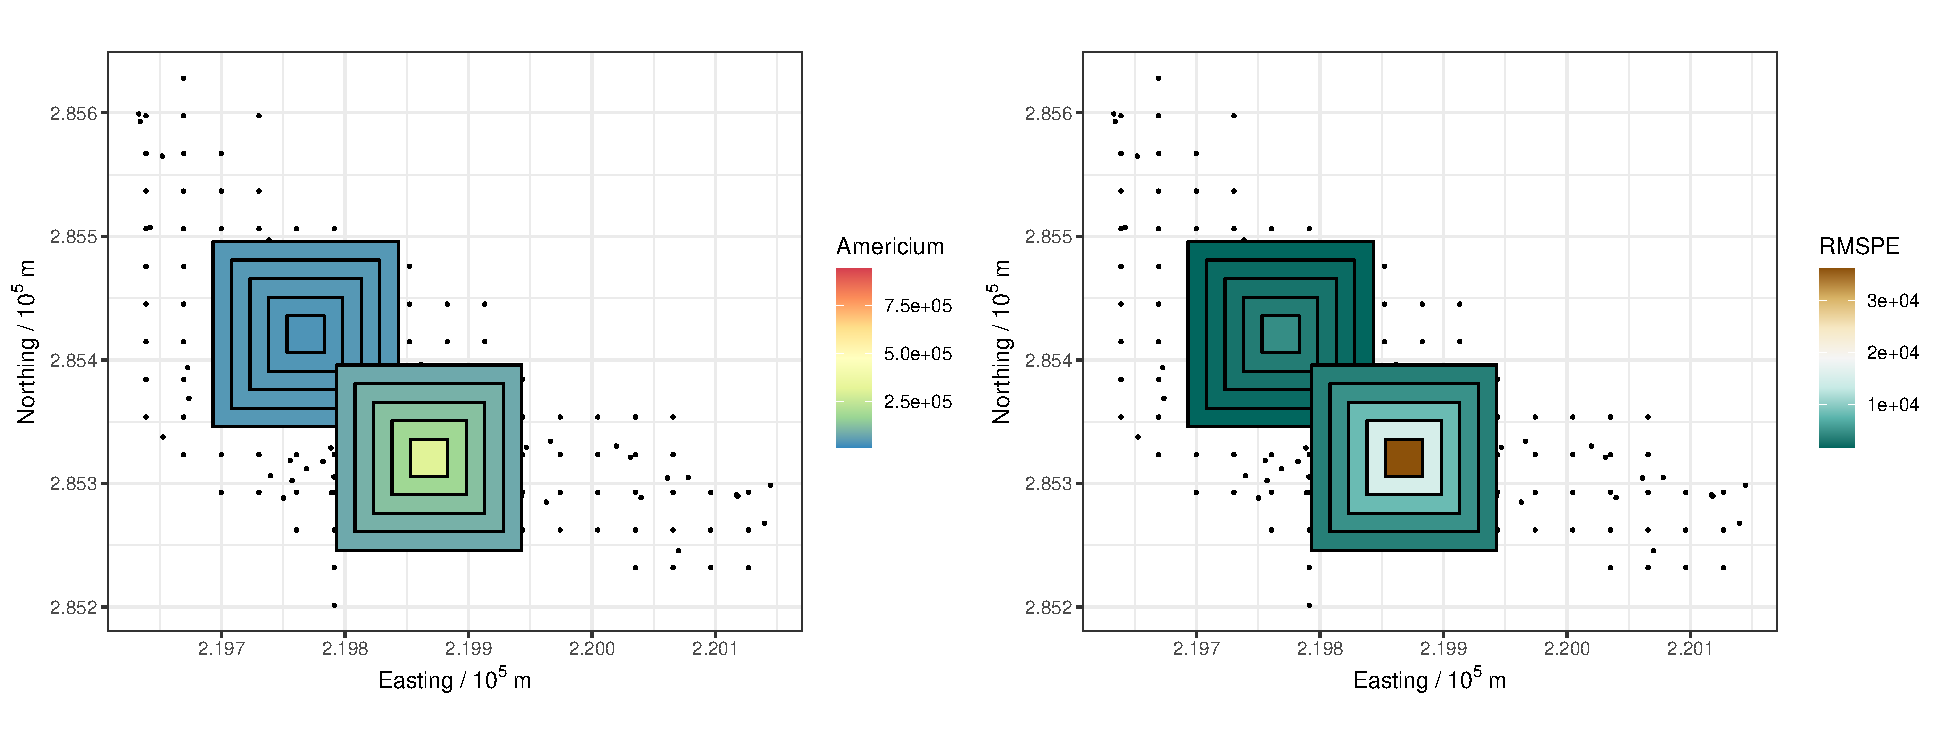
\includegraphics[width = \linewidth]{img/Americium_block_predictions.png}
%     \caption{Block level predictions of the Americium data set. (Left panel) Predictions on the data scale. (Right panel) Block predictions on the log-scale. 
% }   
%   \label{fig:Am_block_predictions}
% \end{figure}













\subsection{Spatial change of support: Poverty in Sydney}\label{sec:spatialCOS}

%%% Original, before data description putting into an appendix:
%The Australian Statistical Geography Standard (ASGS) defines a series of nested geographical areas in Australia known as Statistical Area Levels. 
%Statistical Area Level 1 (SA1) regions have an average population of 400 people each, Statistical Area Level 2 (SA2) regions have an average population of about 10000 people each, and the Statistical Area Level 3 (SA3) regions have a population range of between 30,000 and 130,000 people. 
%SA3 regions are aggregations of SA2 regions, and SA2 regions are aggregations of SA1 regions. 
%For more information on Statistical Areas, see the ASGS webpage (\url{https://www.abs.gov.au/websitedbs/d3310114.nsf/home/australian+statistical+geography+standard+(asgs)}), and for the shapefiles of each Statistical Area Level, see the Australian Bureau of Statistics webpage
%(\url{https://www.abs.gov.au/AUSSTATS/abs@.nsf/DetailsPage/1270.0.55.001July\%202011}).
%In this example, we consider a region of New South Wales containing 7909 SA1 regions, 180 SA2 regions, and 31 SA3 regions, and aim to infer the level of `poverty' (defined below) at the SA1 and SA3 level, just from data at the SA2 level collected in the Census of 2011. 
%Note that data at the SA1 and the SA3 level are available, and we use these to validate our downscaled predictions.
%
%The data consists of the number of families of various types (`couple family with no children', `couple family with children',`one parent family', and `other family') within a range of weekly income brackets.
%For families with a weekly income below $\$1000$ (which, as we explain subsequently, are the families of interest for this analysis), the income brackets are defined in intervals of $\$200$: negative or nil income, 
%% $[\$1;\$199], [\$200;\$399], \dots, [\$800;\$999]$. 
%[\$1--\$199], [\$200--\$399], ..., [\$800--\$999]. 
%To determine the number of families `in poverty' within each Statistical Area, we must define poverty lines. 
%The Melbourne Institute of Applied Economic and Social Research (MIAESR) provided poverty line guidelines for a range of family structures in March 2011 (\url{https://melbourneinstitute.unimelb.edu.au/assets/documents/poverty-lines/2017/Poverty-Lines-Australia-March-Quarter-2011.pdf}).
%Unfortunately, the groupings of our family units do not align exactly with the poverty line definitions as given by the MIAESR, and so, since this example is shown for purely illustrative purposes, we make several assumptions. 
%First, we assume `families with children' consist of exactly two parents and two children.
%Second, since `other families' is difficult to interpret and categorise appropriately in the context of the MIAESR guidelines, we exclude `other families' from the study (less than 2\% of all families). 
%Third, our data do not make clear whether the head of the family is in the workforce; we therefore assume that the head of the family \textit{is} in the workforce, and hence use the first half of Table 1 of the MIAESR guidelines.
%Fourth, our data do not provide exact income figures, but rather income brackets of width \$200; we thus round MIAESR guidelines to the nearest \$200. 
%Hence, the definition of poverty lines (in Australian dollars) for each family unit considered in this study are the weekly incomes of: \$600 for a couple with no children, \$800 for a couple with children, and \$600 for a one parent family. 
%%We do not consider SA2 regions where the total number of families (the size parameter) is equal to zero, as this would cause issues with model fitting.
%%(Note that there is nothing in the framework preventing us from \textit{predicting} over these `empty' SA2 regions, however, for interpretability reasons, we choose not to do so.)
%%In the 31 SA3 regions of interest, there are 10 SA2 regions with zero families; these regions correspond to water reservoirs, industrial areas, Sydney Airport, parks, and cemeteries. 
%Figure \ref{fig:SA2_level_data} shows the SA2 level data used for model fitting.



The Australian Statistical Geography Standard (ASGS) defines a series of nested geographical areas in Australia known as Statistical Area Levels. 
%Statistical Area Level 1 (SA1) regions have an average population of 400 people each, Statistical Area Level 2 (SA2) regions have an average population of about 10000 people each, and the Statistical Area Level 3 (SA3) regions have a population range of between 30,000 and 130,000 people. 
Statistical Area Level 3 (SA3) regions are aggregations of Statistical Area Level 2 (SA2) regions, and SA2 regions are aggregations of  Statistical Area Level 1 (SA1) regions. 
%For more information on Statistical Areas, see the ASGS webpage (\url{https://www.abs.gov.au/websitedbs/d3310114.nsf/home/australian+statistical+geography+standard+(asgs)}), and for the shapefiles of each Statistical Area Level, see the Australian Bureau of Statistics webpage
%(\url{https://www.abs.gov.au/AUSSTATS/abs@.nsf/DetailsPage/1270.0.55.001July\%202011}).
In this example, we consider a region of New South Wales containing 7909 SA1 regions, 180 SA2 regions, and 31 SA3 regions, and aim to infer `poverty' levels at the SA1 and SA3 regions, 
%just from data at the SA2 regions collected in the Census of 2011. 
just from a data set containing mostly SA2 data and a small amount of SA1 data. 
The data was collected in the Census of 2011, and it consists of the number of families of various types within a range of weekly income brackets; we provide further details, and the way in which we define the poverty line for each family type, in Appendix \ref{Appendix:Sydney_data_description}. 
Note that data at the SA1 and the SA3 regions are available, and we use these to validate our down-scaled and up-scaled predictions.  

It is often the case that sampling once from a large area is relatively inexpensive compared to acquiring multiple samples from small areas. 
 Our training data, shown in Figure \ref{fig:SA2_level_data}, is reflective of such a scenario. It includes mostly SA2 regions, but some SA1 regions have also been included. 



\begin{figure}[t!]
    \centering
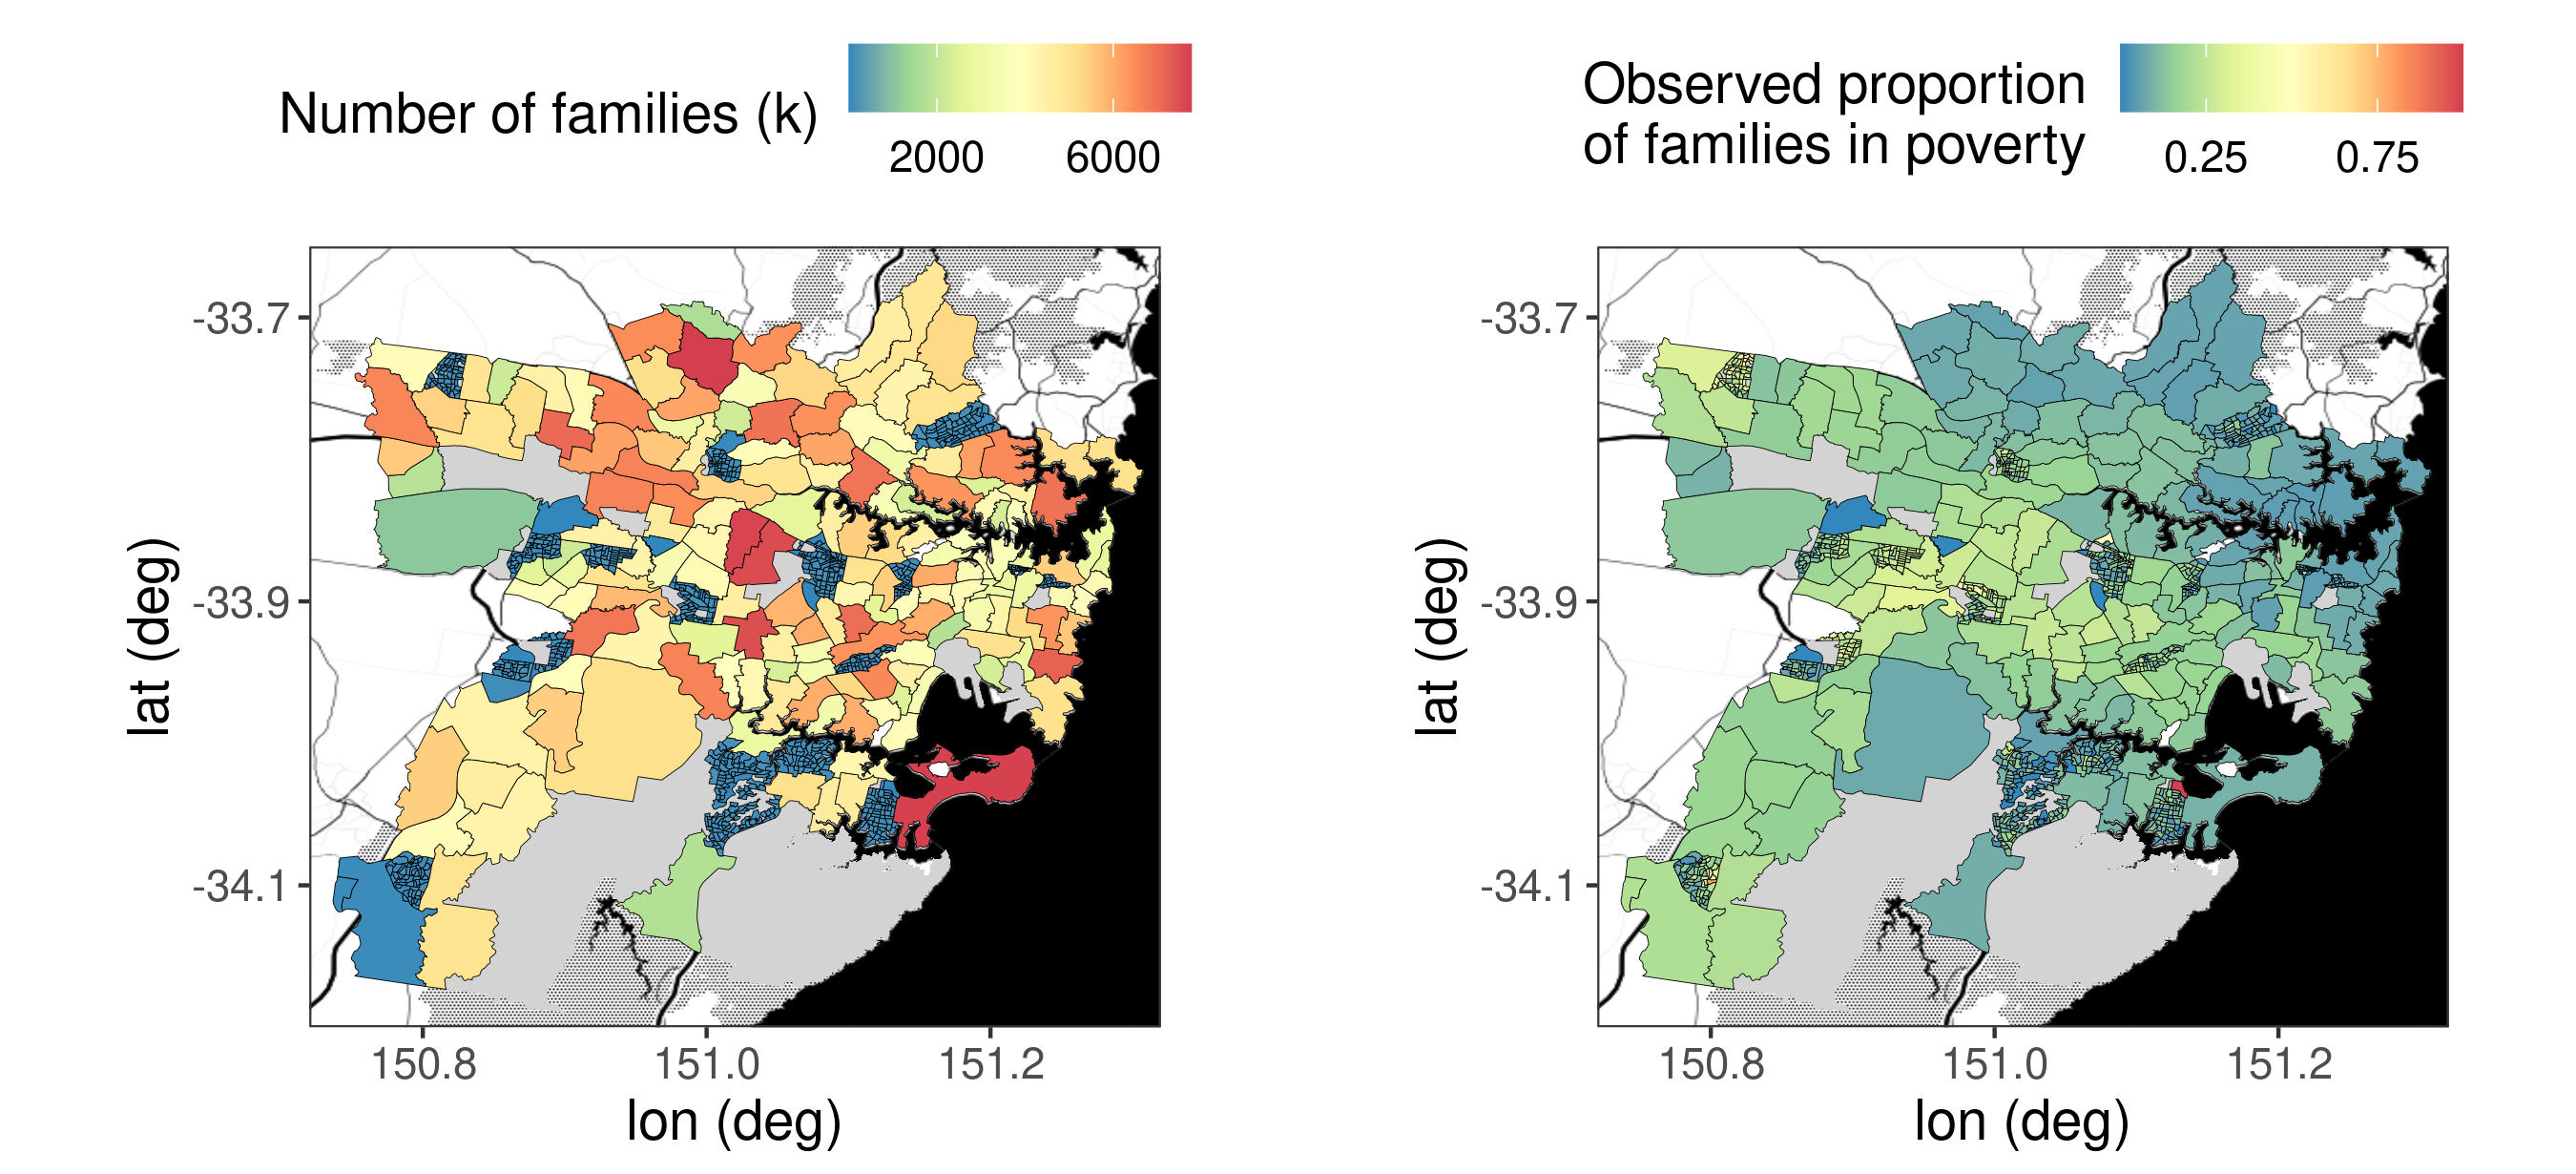
\includegraphics[width = \linewidth]{img/Sydney_training_data.png}
    \caption{
    Training data used for modelling the number (or proportion) of families `in poverty' (see main text for how we define `in poverty'). 
    (Left panel) The total number of families. % at the SA2 level. 
    (Right panel) The observed proportion of families in poverty, % at the SA2 level, 
    computed by dividing the number of families in poverty by the total number of families. Grey regions correspond to SA regions in which the total number of families is zero. 
}   
  \label{fig:SA2_level_data}
\end{figure}



%The first step of an analysis with \pkg{FRK} is to construct and fit the \class{SRE} object using the functions \fct{SRE} and \fct{SRE.fit}, or alternatively with the high-level and user-friendly wrapper \fct{FRK}. 
In this example, we use the SA2 (and some SA1) region data for training the model, and the SA1 regions 
%(no data included) 
as the BAUs; these are passed as \class{SpatialPolygonsDataFrame} objects to \fct{FRK}. 
We also set \code{normalise\_wts = FALSE}, which indicates that we wish to model the mean process in a given 
%SA2 region
data polygon as the sum (rather than the average) of the mean process over the SA1s.
\begin{Code}
R> S <- FRK(f = total_poverty_count ~ 1, 
+    data = list(SA2_and_some_SA1s), BAUs = SA1s, 
+    response = "binomial", link = "logit", normalise_wts = FALSE)
\end{Code}





%The call to fit the \class{SRE} object using the maximum likelihood estimate of the fine-scale variance is:
%\begin{Code}
%S <- SRE.fit(S, method = "TMB", known_sigma2fs = 0.2127)
%\end{Code}
%

% The \code{known\_sigma2fs} argument allows us to fix the fine-scale variance prior to model fitting; this option is particularly useful in a spatial change-of-support setting, when one has a reliable estimate of the fine-scale variance from another source.
Now we predict over the SA1 regions.
\begin{Code}
R> SA1_predictions <- predict(S)
\end{Code}
Since the SA1 regions are the BAUs, we can predict both the probability and mean processes over the SA1 regions: We focus on the probability process, which is independent of the size parameter. 
The predictions and associated uncertainty over the SA1 regions are shown in Figure \ref{fig:SA1_predictions}, which was generated using \fct{plot}.
 \begin{figure}[t!]
    \centering
    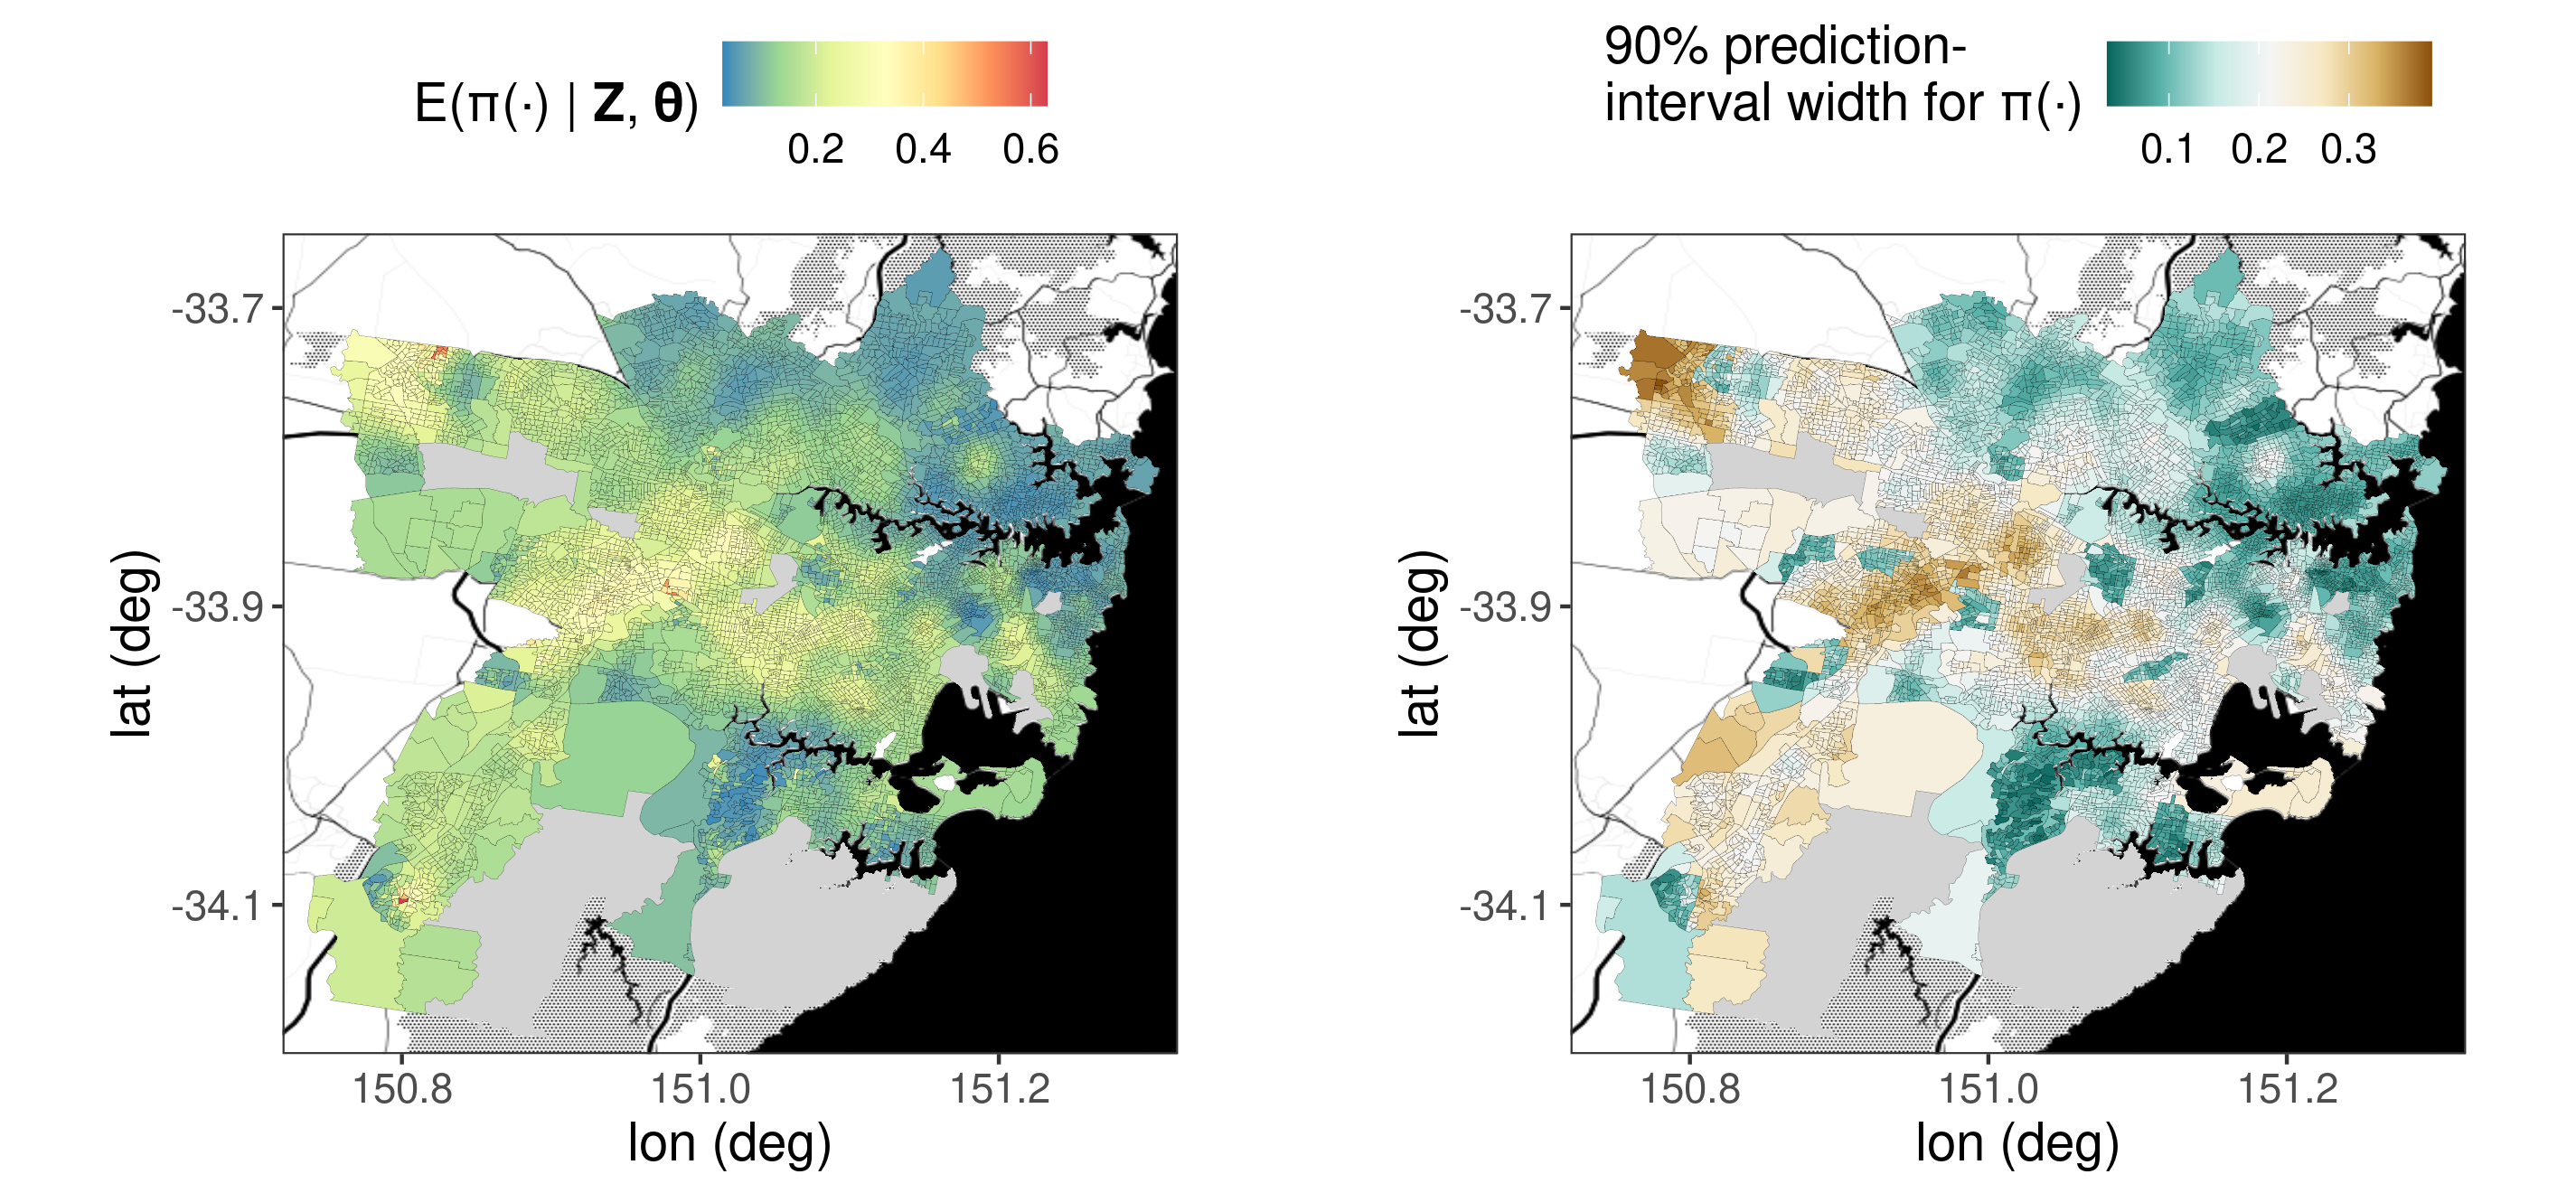
\includegraphics[width = \linewidth]{img/Sydney_SA1_predictions.png}
    \caption{SA1 level predictions. (Left panel) Prediction of the probability process, $\pi(\cdot)$, representing the proportion of families in poverty, over the SA1 regions. (Right panel) 90\% prediction interval width of the probability process.
    Grey regions correspond to SA2 regions in which the total number of families is zero, and hence are omitted from the study. 
}   
  \label{fig:SA1_predictions}
\end{figure}


Predicting over different spatial supports is straightforward with \pkg{FRK} v2. 
 To predict over the SA3 regions, we simply set \code{newdata} to a  \class{SpatialPolygonsDataFrame} object containing the SA3 regions.
\begin{Code}
R> SA3_predictions <- predict(S, newdata = SA3s)
\end{Code}
Figure \ref{fig:SA3_predictions} shows the SA3 region predictions and associated uncertainty quantification: Since the SA3 regions are not the BAUs, this time we are restricted to prediction of the mean process. Again, this graphic was generated using \fct{plot}. 

\begin{figure}[t!]
    \centering
    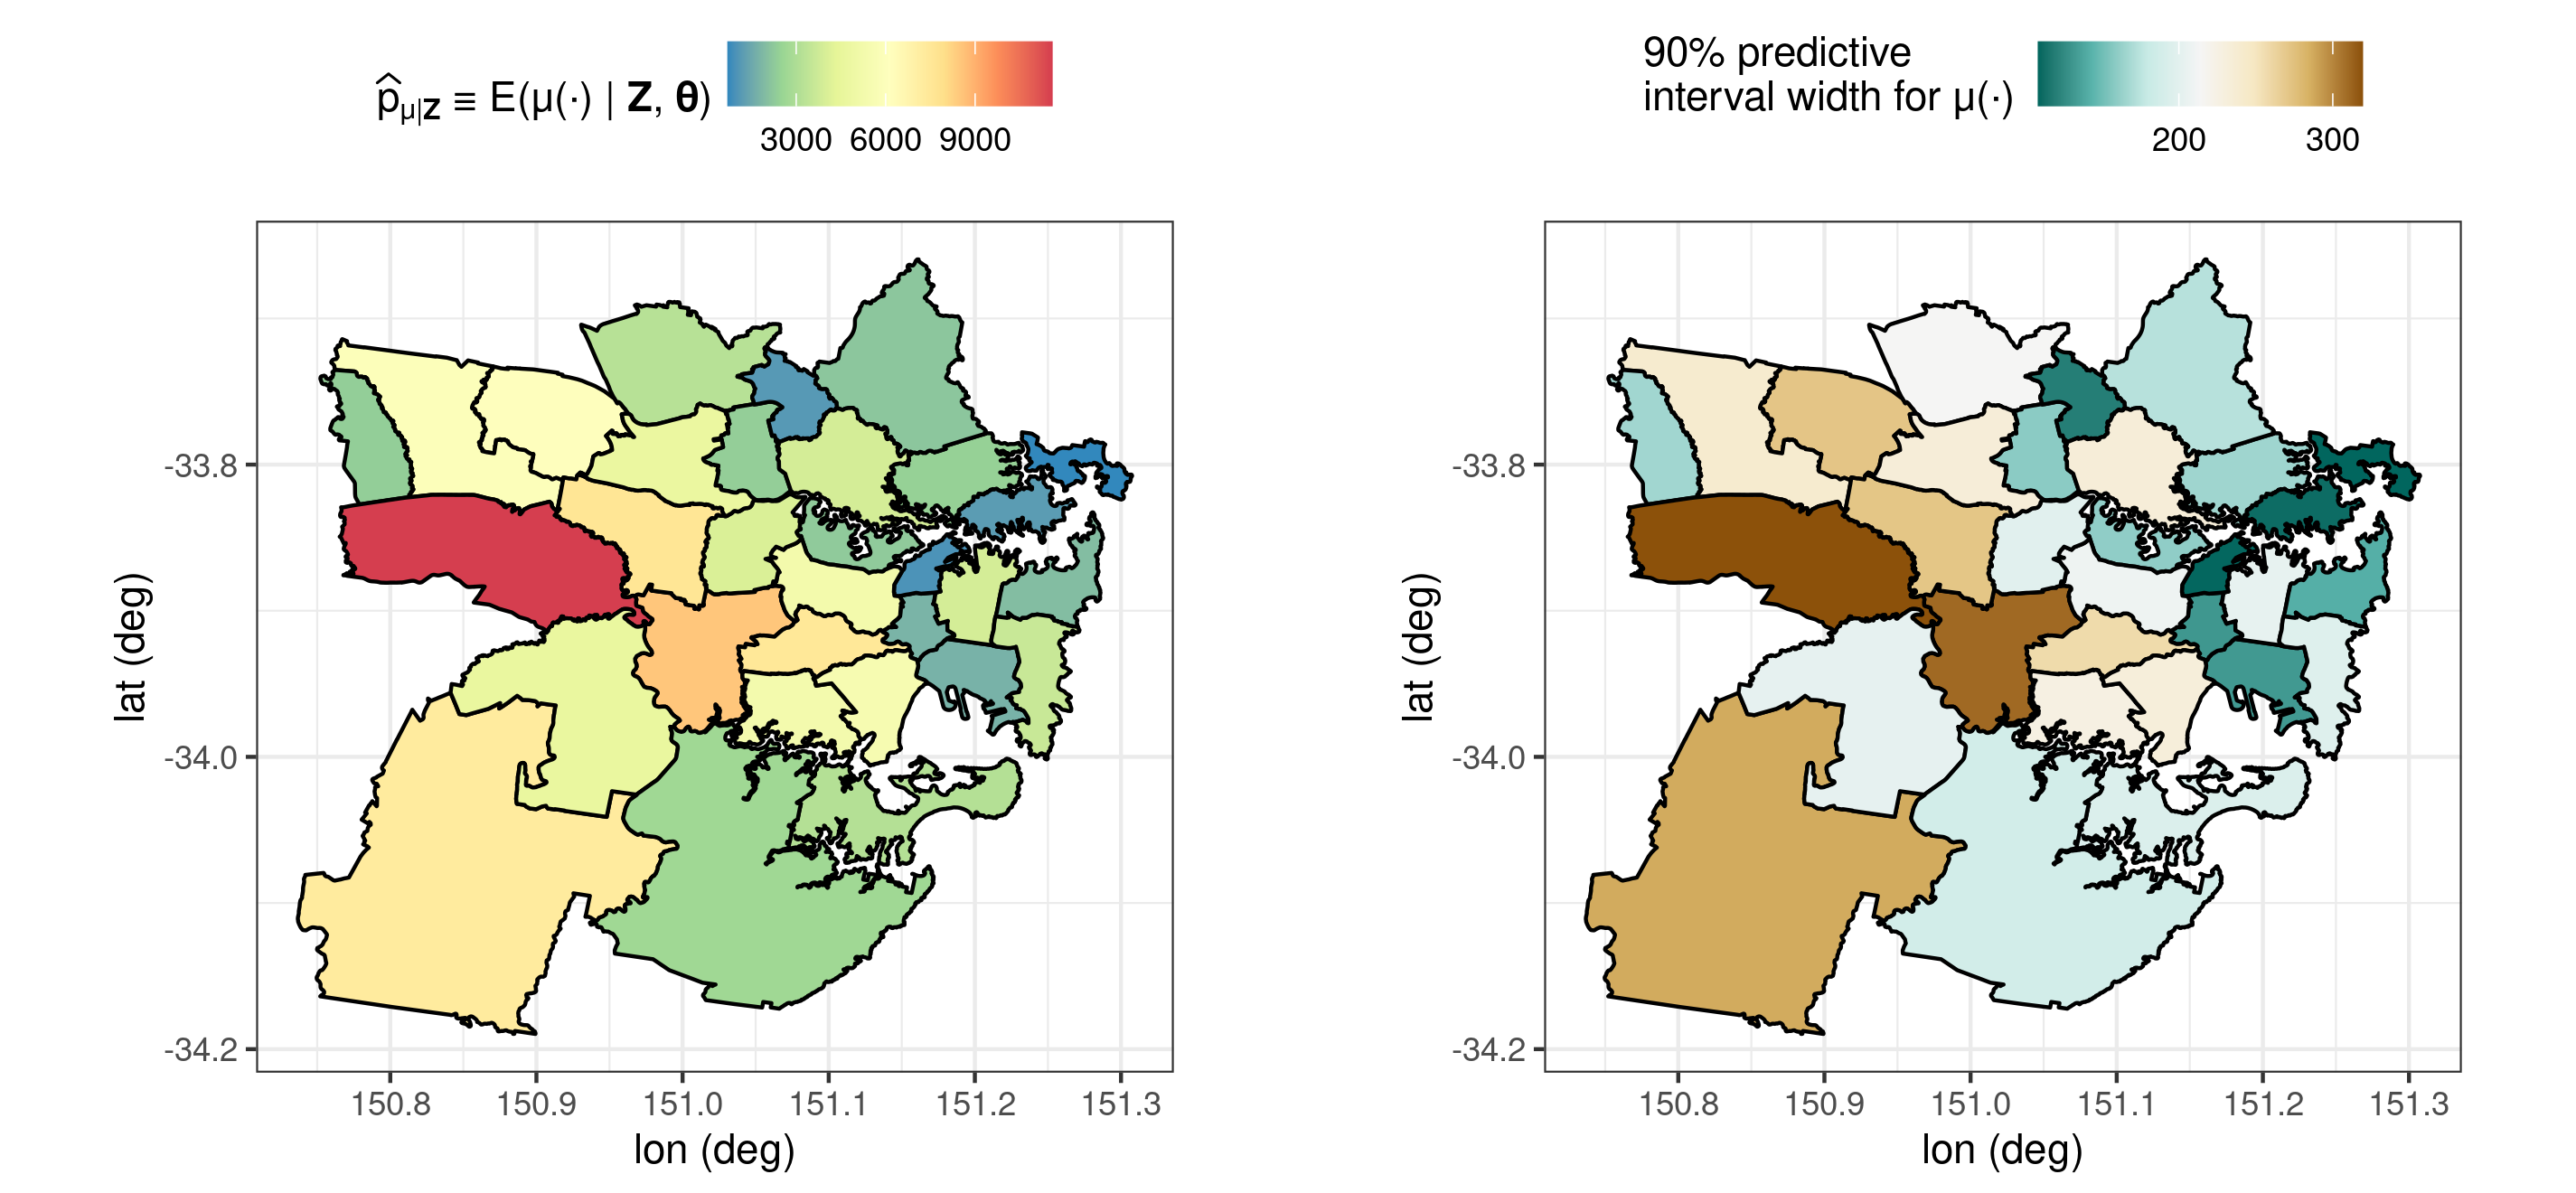
\includegraphics[width = \linewidth]{img/Sydney_SA3_predictions.png}
    \caption{SA3 level predictions. (Left panel) Prediction of the mean process, $\mu(\cdot)$, representing the expected number of families in poverty, over the SA3 regions. (Right panel) The 90\% prediction interval width of the mean process.
}   
  \label{fig:SA3_predictions}
\end{figure}


 We assessed the models ability quantify uncertainty over the SA1 regions by computing the empirical coverage from 90\% prediction intervals. 
 The empirical coverage was 90.8\%, which is almost nominal. 
 The inclusion of some fine-scale data (SA1 region data) greatly aids in the estimation of the fine-scale variance parameter, $\sigma^2_\xi$. 
 If only coarse-resolution data are available (i.e., all data supports are associated with multiple BAUs), in order to avoid identifiability issues, \pkg{FRK} v2 fixes $\sigma^2_\xi$ prior to model fitting with \pkg{TMB}. 
 In this situation, if $\sigma^2_\xi$ is unknown, \pkg{FRK} v2 generates a rough and possibly unreliable estimate. 
 If one does know $\sigma^2_\xi$, or can obtain a reliable estimate of it (for example, using past census data), one may specify it using the argument \code{known\_sigma2fs}. 
 
  

%%Due to issues with identifiability, when the data support is areal with some supports comprising multiple BAUs, \code{method = "TMB"} requires the fine-scale variance parameter, $\sigma^2_\xi$, to be fixed before model fitting. 
%In this situation, if $\sigma^2_\xi$ is unknown, \pkg{FRK} v2 generates a rough estimate. % of it based on the initialisation procedure described in Appendix \ref{appendix:implementation_details}. 
%If one does know $\sigma^2_\xi$, or can obtain a reliable estimate of it, they may specify it using the argument \code{known\_sigma2fs}.
% Using the rough estimate of $\sigma^2_\xi$, we observed an empirical coverage of 82.6\%, which indicates that, at least for this example, the rough estimate is reasonable. 
%As we have SA1 data available, we are able to fit the model using the SA1 regions as both the BAUs \textit{and} the training data, which allows $\sigma^2_\xi$ to be estimated by maximum likelihood estimation; %in this case
%%, although the data are areal, we do not need to fix the fine-scale variance parameter prior to model fitting, because every data support is associated with only a single BAU, and so 
% %we can estimate the fine-scale variance parameter using maximum likelihood estimation. 
% using this maximum likelihood estimate of $\sigma^2_\xi$ improved the coverage to 90.1\%, almost equal to the nominal coverage.
%% In practice SA1 data cannot be used if it is not available; one may use past census data, for example. 
% Hence, if we have a way to obtain a reliable estimate of the fine-scale variance parameter (for example, using past census data), \pkg{FRK} v2 can reliably quantify prediction uncertainty even in a spatial change-of-support setting. 
 
 We conclude this example by noting that, although the prediction polygons, data supports, and BAUs in this study have a nested relationship, in general these elements can be entirely unrelated: Prediction in \pkg{FRK} can be done over any arbitrary, user-specified polygons. See Section \ref{sec:03-03:negative-binomial} for an illustration. 
 

%% A naive predictor of the SA1 level proportion of families in poverty can be obtained by simply assigning the SA2 level proportions to its constituent SA1s. 
%A naive predictor of the proportion of families in poverty at the SA1 level can be obtained by simply computing the observed proportion of families in poverty for a given SA2 region, and then assigning this proportion the SA1 regions which comprise the given SA2 region.
%Such a naive predictor will result in an SA1 level prediction which is identical to the SA2 level training data displayed in the right panel of Figure \ref{fig:SA2_level_data}.
%In the absence of covariate information, predictive performance in spatial change-of-support problems is not necessarily improved by using \pkg{FRK} v2 over a naive predictor. 
%% For instance, the resulting RMSPE when predicting the SA1 level data with \pkg{FRK} v2 was 7.07, whilst the naive predictor scored 7.03.
%However, \pkg{FRK} v2 can provide reliable uncertainty quantification (e.g., the width of predictive intervals), which is important, and difficult to obtain from a naive predictor.
%%Furthermore, the uncertainty quantification quantification provided by \pkg{FRK} v2 is also reliable, as shown by the observed coverage of 90.1\% (when using the `reliable' estimate of the fine-scale variance) and 81.0\% (when using the `rough' estimate of the fine-scale variance) from purported 90\% prediction intervals. 
%\pkg{FRK} v2 also allows covariate information to be considered, the inclusion of which would likely improve prediction over a naive predictor.











\subsection{Non-Gaussian spatio-temporal data: Crime in Chicago}\label{sec:ST_example}


The city of Chicago is divided into 77 so-called community areas (CAs). 
An attractive property of CAs is their relative consistency, their 
boundaries having changed little since their inception in the 1920's \citep{Chicago_library_census_data_info}. 
%Shapefiles for the CAs are available for download from the open data source website, Plenario (\url{http://plenar.io/explore/discover}), or directly from the city of Chicago website (\url{https://data.cityofchicago.org/}). 
In this study, we model the number of crimes in each CA between the years 2001 and 2019.
A full list of crimes committed in 
%the city of 
Chicago during this period is provided by the Chicago Police Department, and is available for download from the open data source website Plenario \citep{Plenario_open_source_website}. 
%The full data set has over 7 million crimes; however, here we consider only violent, non-sexual crimes, which we define as crimes labelled as assault or battery. 
%We considered only violent, non-sexual crimes, which we defined as crimes labelled as assault or battery 
%%(we excluded homicide, which is comparatively rare, with 10,324 recorded instances in our data set).
%(we excluded homicide, which is comparatively rare, accounting for less than 1\% of the violent crimes in our data).
%The data considered in this analysis consisted of 1,748,360 crimes. 
 We considered crimes labelled as assault or battery; 
% 1,748,360 
 roughly 1.75 million crimes in total. 
 Note that \pkg{FRK} bins data falling into the same BAU, so the final number of observations post-binning is significantly less. 
The CA containing O'Hare airport is non-populous and is almost disjoint from the other CAs; for simplicity, we excluded it from this analysis.
% \red{(Noel and Andrew have suggested that we reference \cite{Rodrigues_2010_spatio-temporal_criminology}.)}


In this example, we use the CAs as our spatial BAUs. 
%The CAs, a set of irregular polygons, can be used straightforwardly by reading in the shapefile of the CAs as a \class{SpatialPolygonsDataFrame} object.
This can be done straightforwardly by reading in the shapefile of the CAs as a \class{SpatialPolygonsDataFrame} object. 
Spatio-temporal BAUs may then be constructed by passing the CAs and data into \fct{auto\_BAUs}.
\begin{Code}
R> ST_BAUs <- auto_BAUs(manifold = STplane(), data = chicago_crimes_fit,
+    spatial_BAUs = community_areas, tunit = "years") 
\end{Code}


When modelling crime, it is natural to include population, or population density, as a covariate. 
As the CAs are of unequal area, we use population rather than population density.
%The U.S. Census Bureau does not compile data for CAs; to obtain population data at the CA level, 
This covariate was obtained from the Combined Community Data Snapshots provided by the \cite{Chicago_community_data_snapshots}.
It is difficult to obtain population data for every year, so we assume that population is constant over the time-span of the data.
 We observed a distinct negative trend when plotting the total number of crimes in each year; hence, we also include time as a covariate.
%Figure \ref{fig:chicago_temporal_trend} shows the total number of crimes committed across Chicago in each year, and suggests that a piecewise, linear temporal model split by the year 2014 is appropriate. 
The required BAU level covariates may be constructed in an analogous fashion to 
the way in which the covariates were constructed in 
Section \ref{sec:block_prediction}. 
%\begin{Code}
%ST_BAUs$population <- rep(community_areas$population, times = nt)
%year <- ST_BAUs@data$t + 2000
%ST_BAUs$x1 <- as.numeric(year < 2014)
%ST_BAUs$x2 <- year * ST_BAUs$x1
%ST_BAUs$x3 <- as.numeric(year >= 2014)
%ST_BAUs$x4 <- year * ST_BAUs$x3
%\end{Code}
%
Next, we generate spatio-temporal basis functions automatically using \fct{auto\_basis}.  
% Note that each observation in our data set corresponds to an occurrence of a crime, and these crimes are indexed by the coordinates (longitude, latitude) and date at which the crime occurred; that is, we have unstructured spatio-temporal data in which observations may be recorded at any point in time and location in space. 
%Therefore, we store the full data set, which we label as \mbox{\code{chicago\_crimes}}, as an object of class \class{STIDF}. 
%In a pre-processing step, we aggregated the number of crimes occurring at every unique coordinate and date combination, and stored this number as a field called \mbox{\code{number\_of\_crimes}}; the majority of entries in this field are 1, but it is possible that multiple crimes are recorded at the same location and time (for example, if there are multiple offenders, or if an offender is charged with multiple crimes in the same incident).
%A subset of the \mbox{\code{chicago\_crimes}} data, specifically, all of the data excluding the years 2010 and 2019, was used for training the model and automatically constructing the basis functions. %; this training subset is labelled \mbox{\code{chicago\_crimes\_fit}}.
\begin{Code}
R> basis <- auto_basis(STplane(), chicago_crimes_fit, tunit = "years")
\end{Code}
%Once the BAUs and basis functions are constructed, we use \fct{SRE} to initialise the \class{SRE} object, specifying \code{response = "poisson"} and \code{link = "log"}.
Then, we initialise and fit the \class{SRE} object using \fct{FRK}, setting \code{response = "poisson"} and \code{link = "log"}. 
%\marginnote{\code{link = "sqrt"} would be better, for computational and interpretation reasons. Plus it is non-canonical.}
 Each entry of our data provides the location and time at which a given crime occurred. It also contains a column of ones called \code{"number\_of\_crimes"}; this will be used for binning. 
 By default, \fct{SRE}, which is called internally within \fct{FRK}, bins and then averages data falling into the same BAU. 
 We wish to model the total number of crimes in a given BAU; hence, we wish to sum the binned data instead of average. To do so, we pass the name of the response variable (\code{"number\_of\_crimes"}) via the argument \code{sum\_variables}.
As the number of spatial BAUs (the CAs) is relatively low, and we have observed each spatial BAU multiple times, we may attribute each spatial BAU its own fine-scale variance parameter (see Section \ref{sec:spatio-temporal}). % by setting \code{fs\_by\_spatial\_BAU = TRUE}.
\begin{Code}
R> S <- FRK(f = number_of_crimes ~ log(population) + x1 + x2 + x3,   
+    data = list(chicago_crimes_fit), basis = basis, BAUs = ST_BAUs,         
+    response = "poisson", link = "log", 
+    sum_variables = "number_of_crimes", fs_by_spatial_BAU = TRUE) 
\end{Code}
Finally, we predict over the spatio-temporal BAUs (which use the CAs as spatial BAUs) using \fct{predict}, and plot the results using \fct{plot}.
%\begin{Code}
%pred <- predict(S)
%
%subset_time <- c(2010, 2019) 
%plots <- plot(S, pred$newdata, binned_data, 
%              map_layer = chicago_map, subset_time = subset_time, 
%              colour = "black", size = 0.3, alpha = 0.85)
%
%plots <- lapply(plots, function(gg) gg + 
%                  facet_wrap(~t,  ncol = 1) + 
%                  xlab("lon (deg)") + ylab("lat (deg)"))
%                  
%ggpubr::ggarrange(
%  plots$number_of_crimes, plots$p_Z, plots$interval_90_Z, 
%  align = "hv", nrow = 1, legend = "top"
%)
%\end{Code}



\begin{figure}[t!]
    \centering
    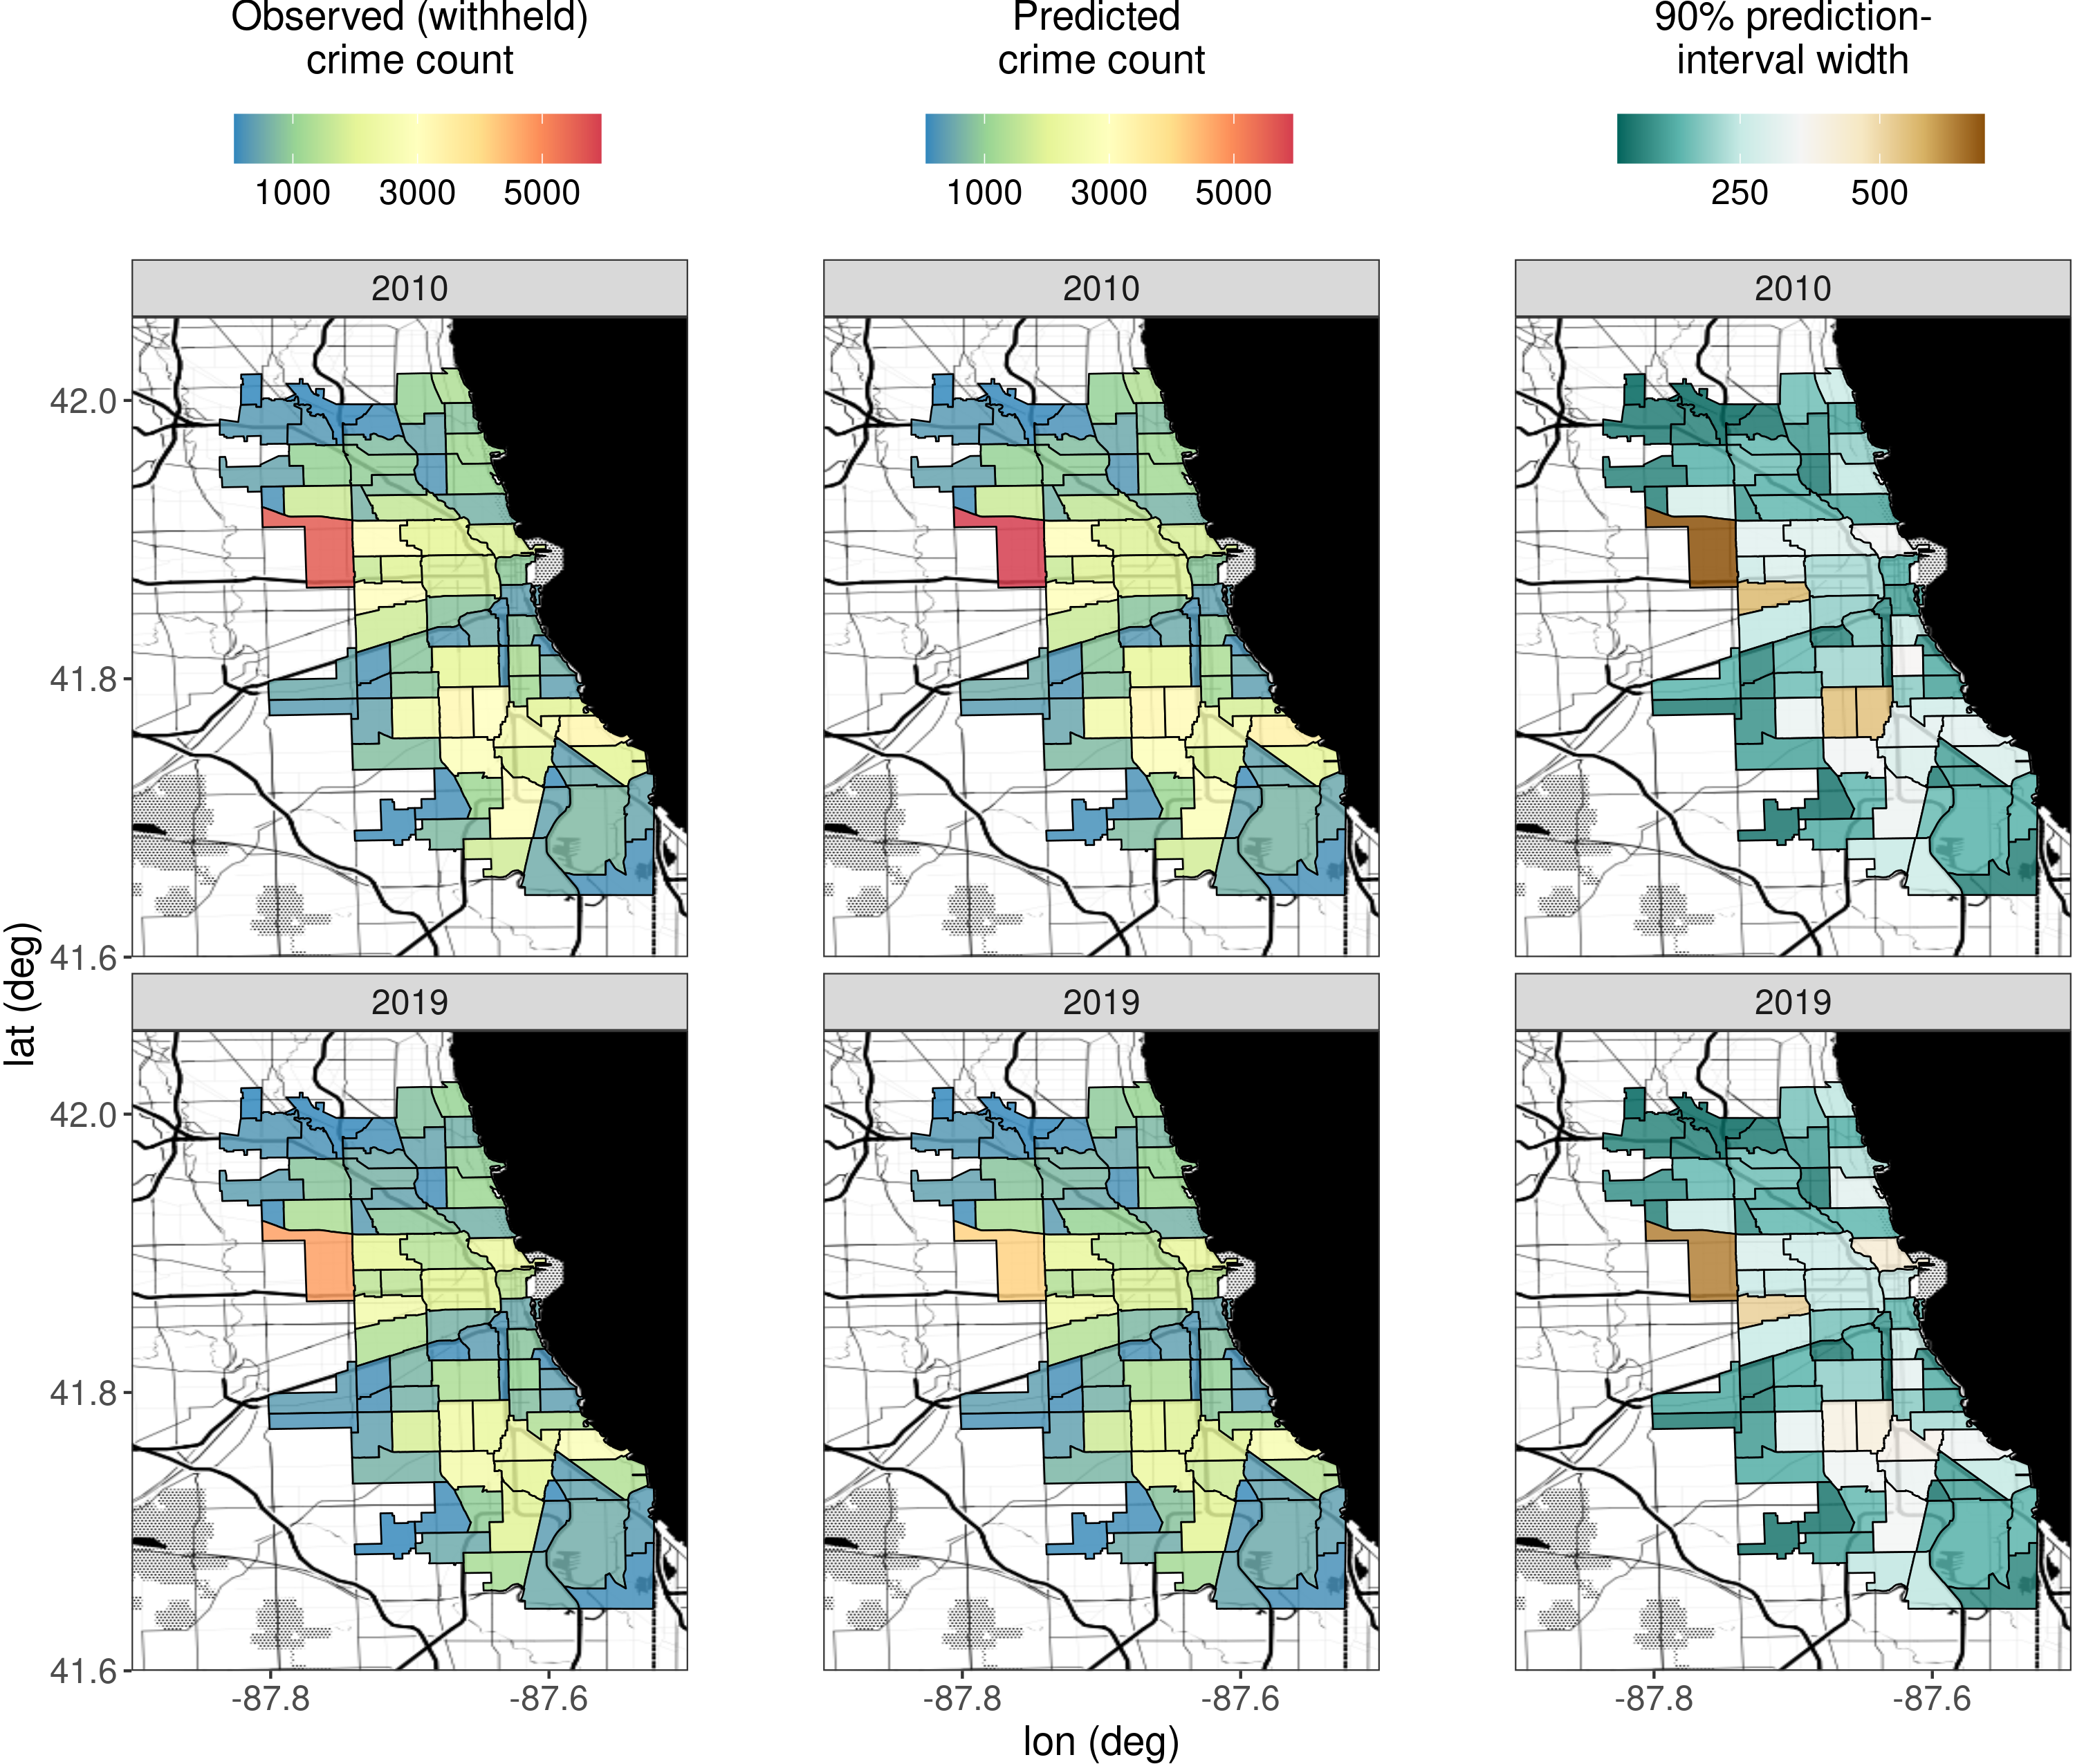
\includegraphics[width = \linewidth]{img/Chicago_data_pred_uncertainty.png}
    \caption{Observed number of crimes, predictions, and prediction uncertainty over 
%    the city of 
    Chicago in the prediction (2010) and forecast (2019) years. The first row corresponds to the year 2010; the second row corresponds to the year 2019. The first column shows the observed number of crimes; the second column shows the predicted number of crimes; the third column shows the width of a posterior predictive interval with a purported coverage of 90\%.%, which acts as a measure of uncertainty on the predictions.
}   
  \label{fig:chicago_validation_predictions}
\end{figure}








\begin{figure}[t!]
    \centering
    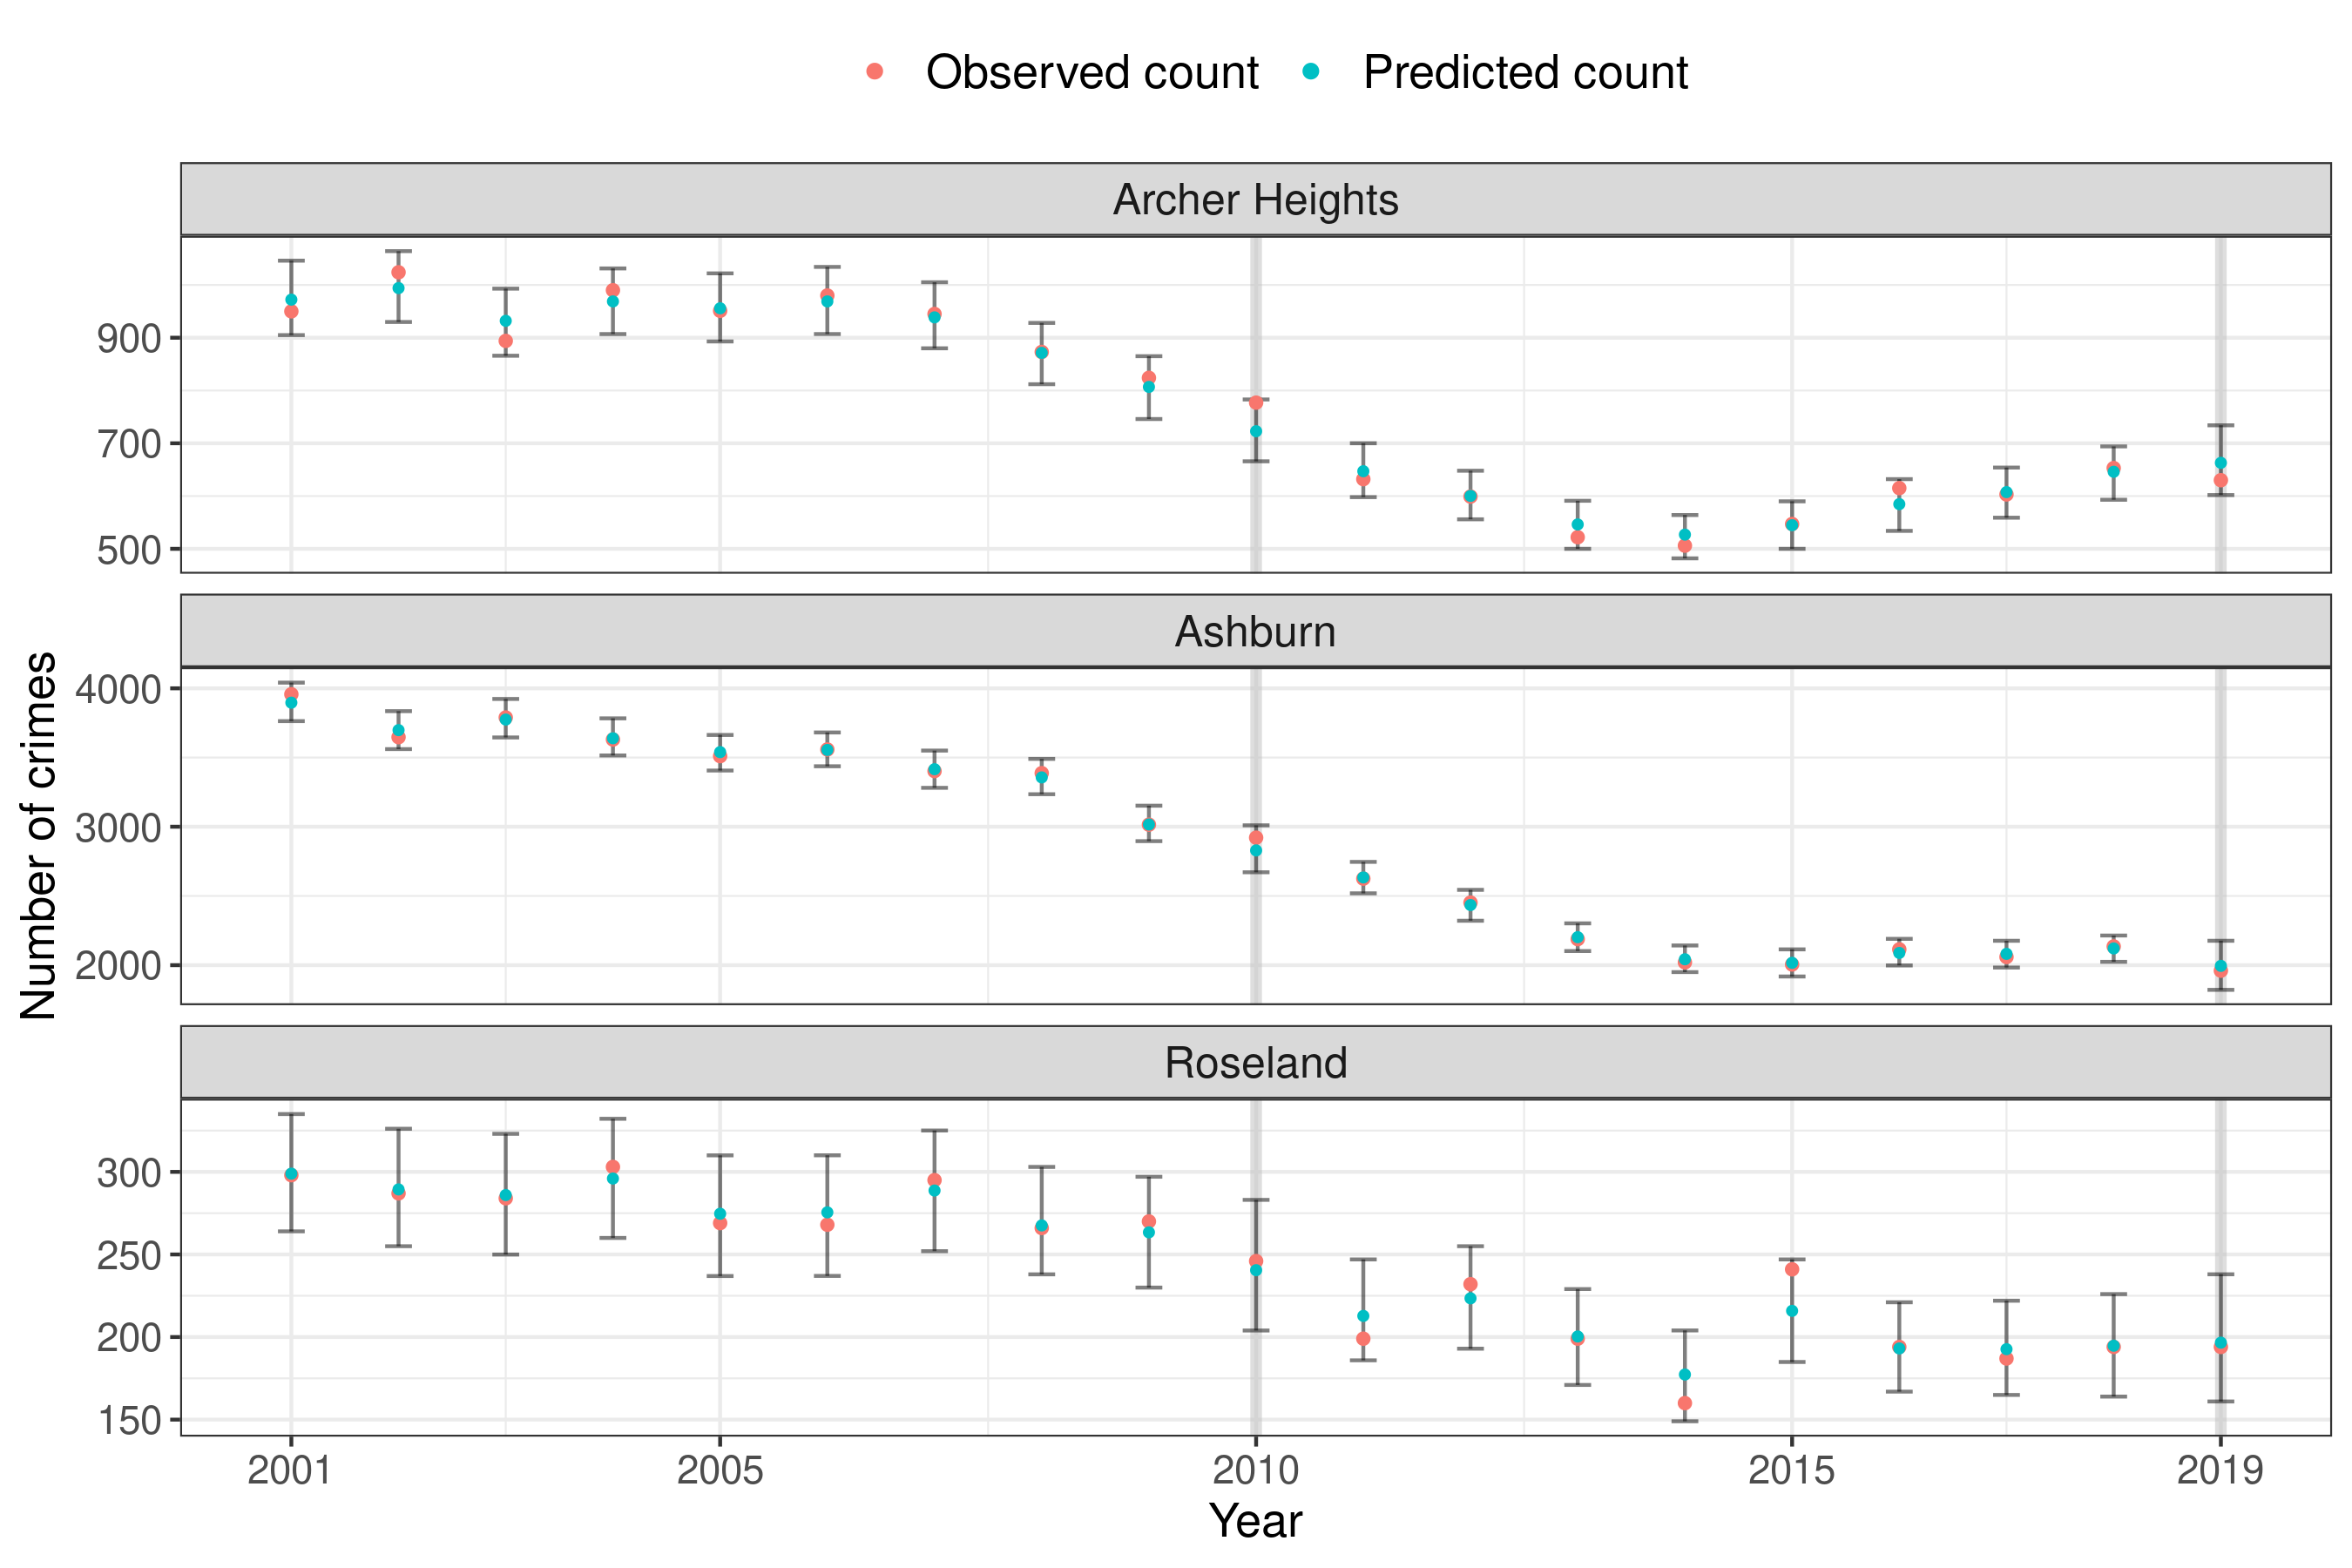
\includegraphics[width = \linewidth]{img/Chicago_focused_CAs_time_series.png}
    \caption{Time-series plots of predictions and observed number of crimes for three CAs of interest. The validation years, 2010 and 2019, are highlighted in light-grey. The observed number of crimes at each time is indicated by a red point, whilst the predicted number of crimes is indicated by a blue point. The error bars represent a 90\% posterior predictive interval. We note that the posterior predictive intervals are slightly wider in validation years (2010 and 2019) than in observed years, and that the observed crime is contained within the predictive interval for all time-points for these CAs. 
}   
  \label{fig:chicago_time_series}
\end{figure}

\begin{figure}[t!]
    \centering
    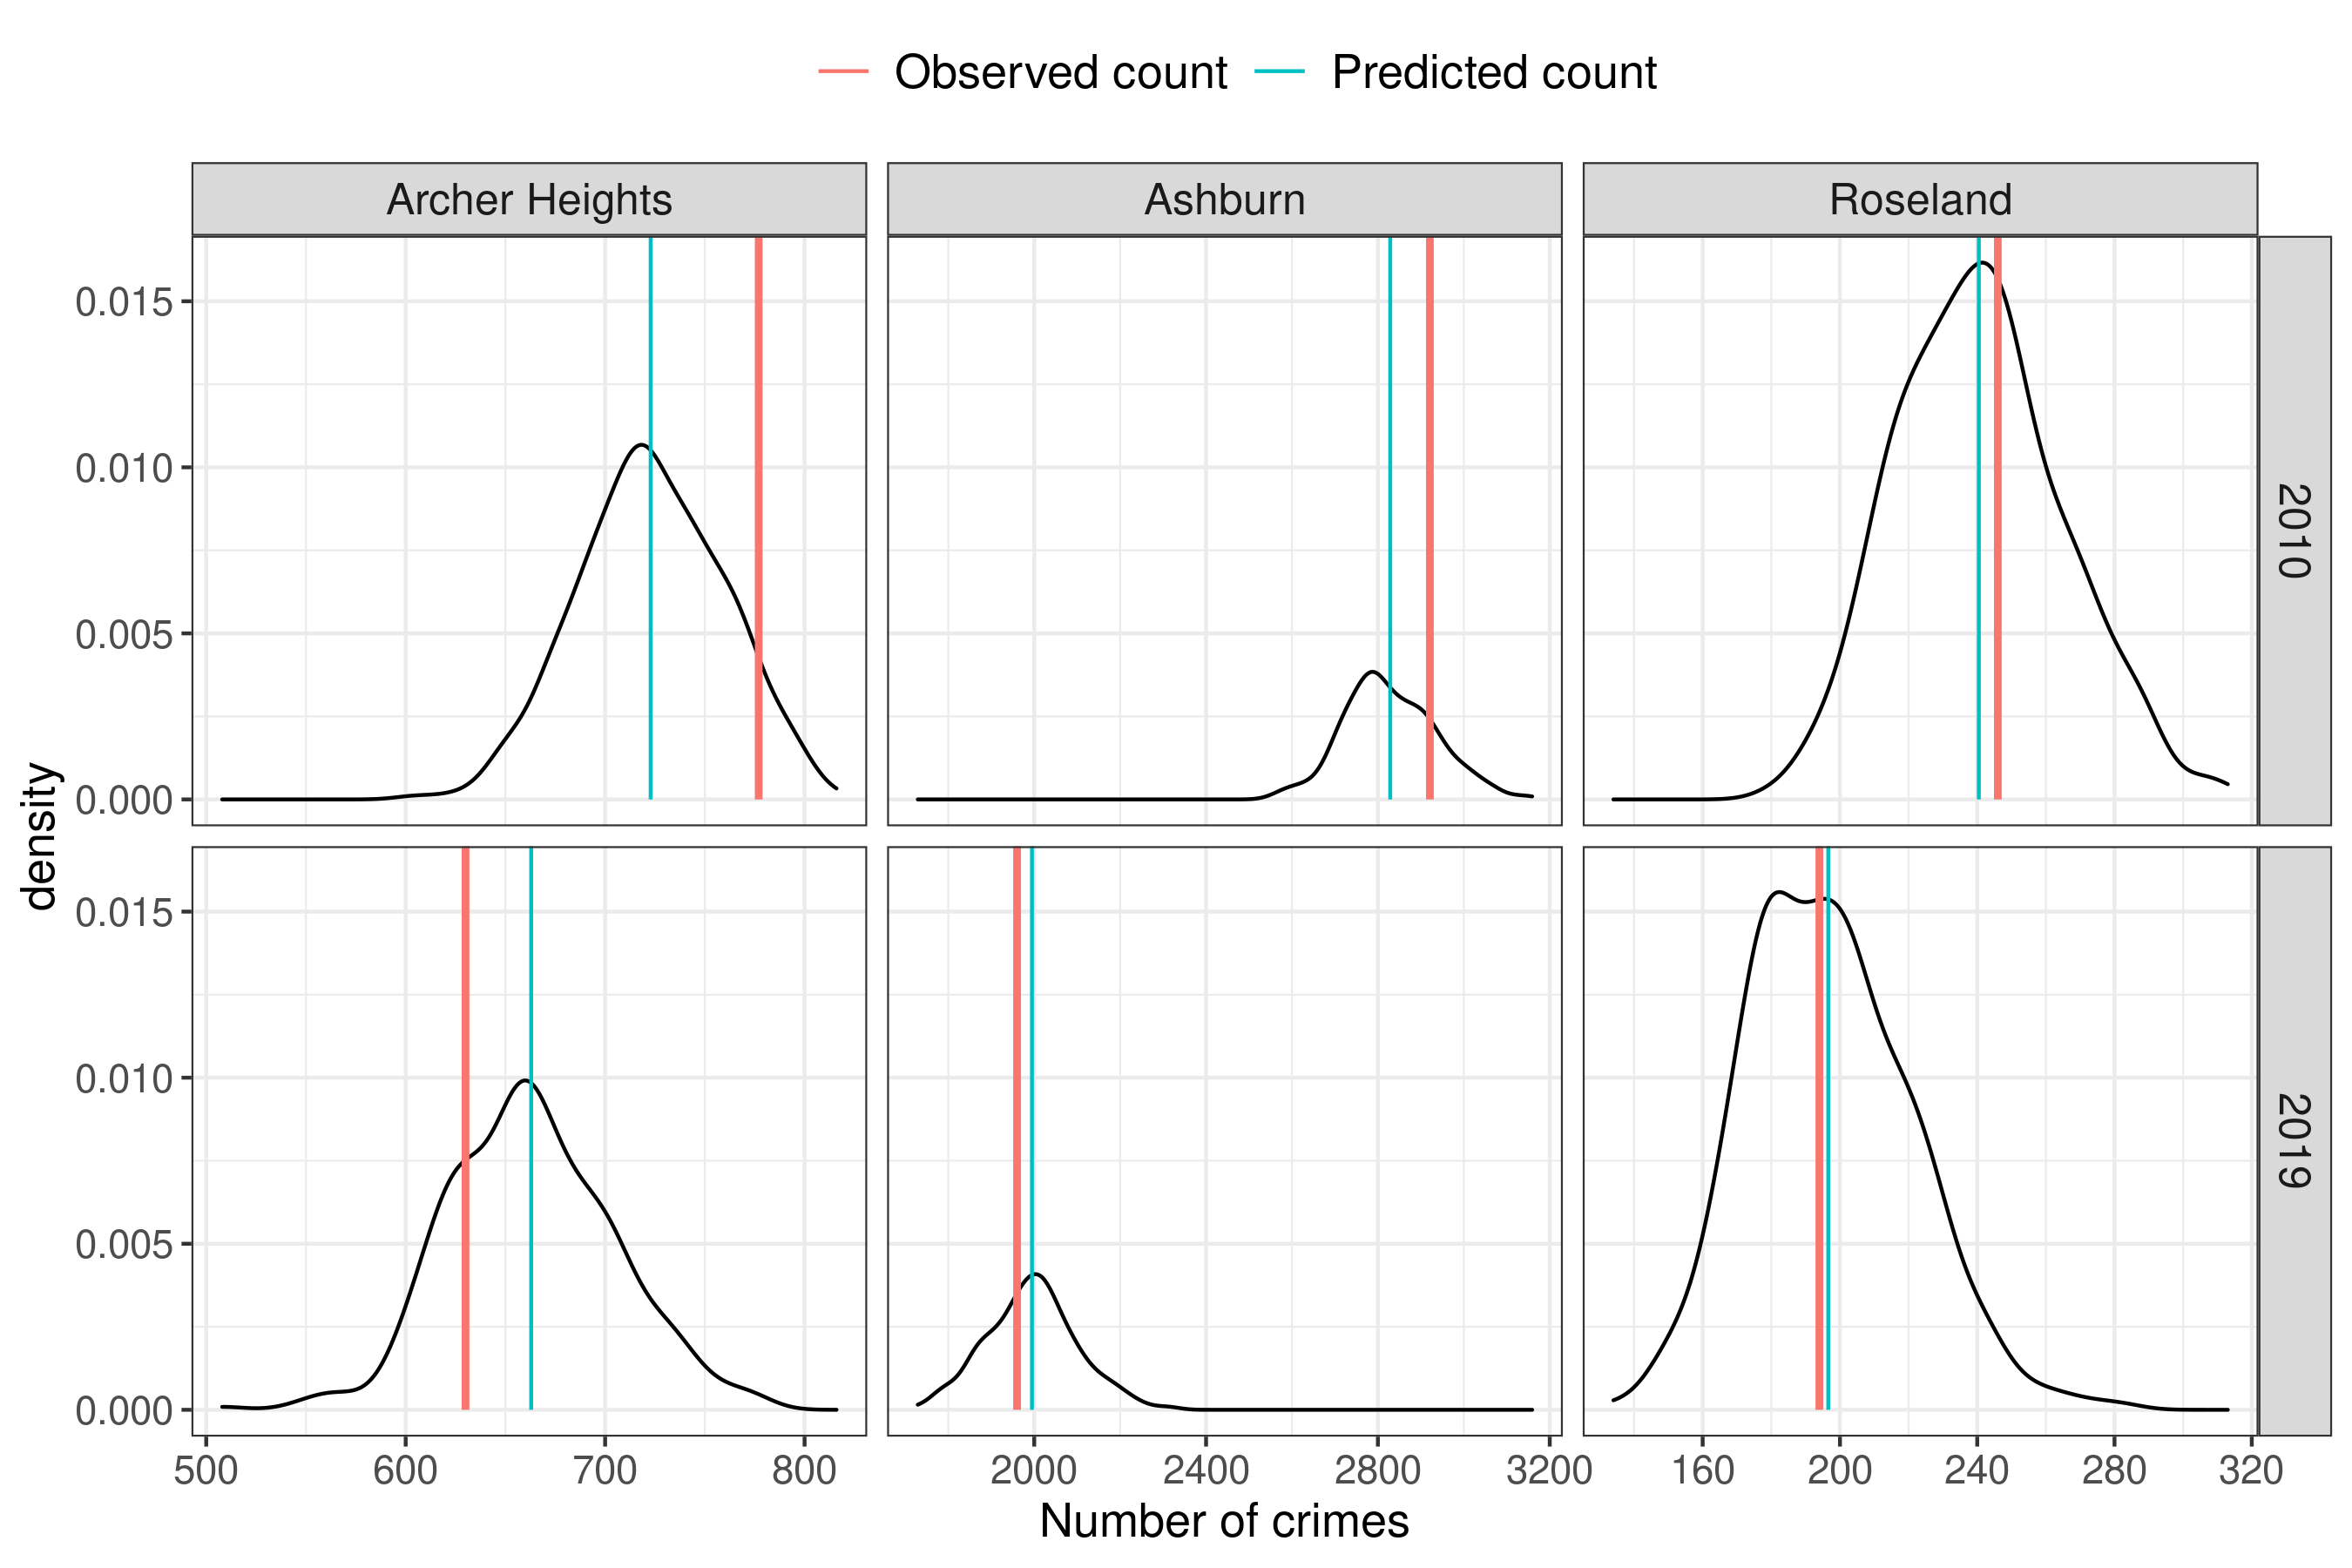
\includegraphics[width = \linewidth]{img/Chicago_focused_CAs_predictive_distributions.png}
    \caption{Posterior predictive distributions in the validation years (2010 and 2019) for three CAs (Archer Heights, Ashburn, and Roseland). The red and blue lines correspond to the observed and predicted number of crimes at each CA in the given year. 
    The first \textit{row} corresponds to the year 2010; the second row corresponds to the year 2019. The first \textit{column} corresponds to Archer Heights; the second column corresponds to Ashburn; the third column corresponds to Roseland. 
}   
  \label{fig:chicago_predictive_distributions}
\end{figure}


To validate predictions, we excluded the years 2010 and 2019 from the training data. 
The observed number of crimes, predicted number of crimes, and prediction uncertainty for these years are provided in Figure \ref{fig:chicago_validation_predictions}. 
For both years, Figure \ref{fig:chicago_validation_predictions} shows agreement between the predicted and observed number of crimes. Furthermore, 
%we can observe a distinct relationship between the prediction and the prediction uncertainty; specifically, 
 the prediction uncertainty is roughly proportional to the predicted value, as one may expect when modelling counts.
For these validation years, we also computed the empirical coverage when using 90\%, 80\%, 70\%, and 60\% posterior predictive intervals, and the mean absolute percentage error (MAPE; see Appendix \ref{app:ScoringRules}). 
We consistently observed that the empirical coverage in the year 2010 was slightly (4\% on average) higher than the purported coverage, whilst it was lower (16\% on average) in the forecast year.
% For these validation years, we also computed the empirical coverage when using 90\%, posterior predictive intervals, and the mean absolute percentage error (MAPE; see Appendix \ref{app:ScoringRules}). 
% We empirical coverage in the year 2010 was slightly higher (94.7\%) than the purported coverage, whilst it was lower (76.3\%) in the forecast year. 
We observed MAPE scores of 4.4\% and 9.0\% in the years 2010 and 2019, respectively.
The slightly worse results in the year 2019 is possibly expected, as forecasting into the future is, in general, a harder task than predicting within the time-span of the data.
Nonetheless, these predictions are cause for optimism given the difficulties in modelling crime in a spatio-temporal setting. 


For illustration, we chose three CAs of interest: 
%these CAs are 
Ashburn, % (CA 70), 
Roseland, % (CA 49), 
and Archer Heights. % (CA 57).
The time-series of the observed data, predictions, and 90\% posterior predictive intervals for these CAs is shown in Figure \ref{fig:chicago_time_series}. 
The posterior predictive intervals are slightly wider in validation years (2010 and 2019) than in observed years. 
 The observed number of crimes is contained within the predictive interval for all time-points for these CAs.
The predictive distributions in the validation years for the three CAs of interest is shown in Figure \ref{fig:chicago_predictive_distributions}.
The forecasts for Ashburn and Roseland in the year 2019 are particularly accurate, with the predicted number of crimes essentially equal to the observed number of crimes. 



\section{Conclusion}
\label{SEC:Conclusion}


In this paper we have described an extension to the \proglang{R} package \pkg{FRK} which allows for the spatial and spatio-temporal modelling and prediction of big, non-Gaussian data. 
Thanks to the use of a GLMM model and the software \pkg{TMB}, \pkg{FRK} v2 can now cater for many distributions within the exponential family, and many link functions. 
Furthermore, \pkg{FRK} v2 allows for the use of many more basis functions when modelling the spatial process, and can therefore also often achieve more accurate predictions in a Gaussian setting than \pkg{FRK} v1. 
The existing functionality of \pkg{FRK} is retained with this extension; in particular, the package makes use of automatic basis function construction, is capable of handling both point-referenced and areal data, and eases the so-called spatial change-of-support problem through the use of BAUs.
The package now provides a highly accessible and user friendly approach to spatial and spatio-temporal modelling of big data in both a Gaussian and non-Gaussian setting.


One limitation of the framework is that it requires covariates to be known for every BAU, which may not be the case if covariates are recorded only at the data support level.
 Another limitation is the necessity to fix the fine-scale variance parameter in spatial change-of-support applications when \code{method = "TMB"}; note that this is not an issue if one is able to obtain a reliable estimate through other means (e.g., via previous census data). 
 We are currently exploring avenues to address this limitation, either through adjusting the model to allow estimation of the fine-scale variance parameter within \pkg{TMB}, or via a more robust offline estimate.
Another limitation is that despite the added flexibility, several models of interest, such as the zero-inflated Poisson, are still not catered for. 
 The introduction of different types of models is facilitated by \pkg{TMB}'s implementation of automatic differentiation, which means we can make use of existing code within the \proglang{C++} template straightforwardly; future work will see the introduction of other models of interest.   
 The main spatial data structures used in \pkg{FRK} come from the package \pkg{sp} \citep{Pebesma_2005_sp_package}; future work may entail the inclusion of other spatial data structures, such as those from the package \pkg{sf} \citep{Pebesma_2018_sf_package}.
% Another is that, because of the separability of basis functions between space and time, the framework cannot capture interactions between space and time \citep[][Ch.~5]{Wikle_2019_ST_stats_with_R}. 
% (Mathematically, it can, but in practice, due to the compact support of the basis functions, the implied fields from the model are 'pseudo-stationary'.)


\section*{Acknowledgments}

Matthew Sainsbury-Dale's research was supported by an Australian Government Research Training Program Scholarship.
Andrew Zammit-Mangion's and Noel Cressie's research was supported by an Australian Research Council (ARC) Discovery Project, DP190100180. Andrew Zammit-Mangion's research was also supported by an ARC Discovery Early Career Research Award, DE180100203.  
The authors would like to thank Rajib Paul for providing the Americium data analysed in Section \ref{sec:block_prediction}, 
%Dr.~Matt Moores for discussion on the ethics of modelling crime in the city of Chicago, 
and Michael Bertolacci for discussion surrounding the MODIS comparison study.








%% -- Bibliography -------------------------------------------------------------
%% - References need to be provided in a .bib BibTeX database.
%% - All references should be made with \cite, \citet, \citep, \citealp etc.
%%   (and never hard-coded). See the FAQ for details.
%% - JSS-specific markup (\proglang, \pkg, \code) should be used in the .bib.
%% - Titles in the .bib should be in title case.
%% - DOIs should be included where available.

\bibliography{FRKv2}


%% -- Appendix (if any) --------------------------------------------------------
%% - After the bibliography with page break.
%% - With proper section titles and _not_ just "Appendix".

%% Supp Material
%\renewcommand{\thefigure}{S\arabic{figure}}
%\setcounter{figure}{0}   
%\section{Supplementary material and figures}

%In this section we provide supplementary material and figures which were omitted from the main body for the sake of brevity. 

%Figure \ref{fig:BAU_intuition} is included to provide intuition on how BAUs are used within \pkg{FRK}.
%It shows how the continuous spatial domain $D$ is discretised into basic areal units (BAUs), the kind of supports permitted in \pkg{FRK} (both areal and point-referenced), and how the observation domain is constructed through observation supports. Figure \ref{fig:Poisson_multires} displays the prediction and prediction uncertainty when using a varying number of basis function resolutions, where the data used for model fitting is the point-referenced data set shown in Figure \ref{fig:Poisson_true_and_Z}. Figure \ref{fig:chicago_temporal_trend} demonstrates that the period before 2014 exhibits a different temporal trend to the period after 2014 in terms of the number of crimes committed in Chicago. 




%\begin{figure}[t!]
%\centering
%\begin{tikzpicture}
%% Continuous domain D
%\begin{scope}[xshift = -4cm]
%\node at (1.5,4.5) {$D$};
%\draw (0, 0) rectangle (3, 4);% node [below left] {$D$};
%\end{scope}
%% Discretised domain, D^G
%\node at (1.5,4.5) {$D^G$};
%\draw[step=1cm] (0,0) grid (3,4);
%\node at (0.5,3.5) {$A_1$};
%\node at (1.5,3.5) {$A_2$};
%\node at (2.5,3.5) {$A_3$};
%\node at (0.5,2.5) {$A_4$};
%\node at (1.5,2.5) {$A_5$};
%\node at (2.5,2.5) {$A_6$};
%\node at (0.5,1.5) {$A_7$};
%\node at (1.5,1.5) {$A_8$};
%\node at (2.5,1.5) {$A_9$};
%\node at (0.5,0.5) {$A_{10}$};
%\node at (1.5,0.5) {$A_{11}$};
%\node at (2.5,0.5) {$A_{12}$};
%% Discretised domain, D_G, with observations
%\begin{scope}[xshift = 4cm]
%% \node at (1.5,4.5) {$D^O$};
%\draw[step=1cm] (0,0) grid (3,4);
%\filldraw[color=red, fill=red, opacity = 0.7] (0.25, 3.75) rectangle (1.1, 2.25);
%\filldraw[color=red, fill=red, opacity = 0.7] (0.15, 0.15) rectangle (1.85, 0.9);
%\filldraw[red, opacity = 0.7] (2.75,2.75) circle (0.08cm);
%\node at (0.5,3.5) {$A_1$};
%\node at (1.5,3.5) {$A_2$};
%\node at (2.5,3.5) {$A_3$};
%\node at (0.5,2.5) {$A_4$};
%\node at (1.5,2.5) {$A_5$};
%\node at (2.5,2.5) {$A_6$};
%\node at (0.5,1.5) {$A_7$};
%\node at (1.5,1.5) {$A_8$};
%\node at (2.5,1.5) {$A_9$};
%\node at (0.5,0.5) {$A_{10}$};
%\node at (1.5,0.5) {$A_{11}$};
%\node at (2.5,0.5) {$A_{12}$};
%\end{scope}
%% observation supports
%\begin{scope}[xshift = 8cm]
%\node at (1.5,4.5) {$D^O$};
%\draw[step=1cm] (0,4) grid (1,2);
%\draw[step=1cm] (0,0) grid (2,1);
%\draw[step=1cm] (2,2) grid (3,3);
%\node at (0.5,3.5) {$A_1$};
%\node at (0.5,2.5) {$A_4$};
%\node at (2.5,2.5) {$A_6$};
%\node at (0.5,0.5) {$A_{10}$};
%\node at (1.5,0.5) {$A_{11}$};
%
%\end{scope}
%\end{tikzpicture}
%\caption{A toy example demonstrating discretisation of the continuous spatial domain, and how the observation domain is derived from observations.
%(Left panel) The continuous spatial domain, $D$.
%(Centre-left panel) The discretised version of the spatial domain, $D^G$; in this example, $N = 12$ BAUs are used to tile the domain. 
%(Centre-right panel) The discretised domain after observing $m$ footprints; here, we have $m = 3$ footprints, two of which are areally referenced rectangles, while one is point referenced. 
%(Right panel) The observation domain, $D^O$; the observation supports which comprise $D^O$ are $B_1 = A_1 \cup A_4$,  $B_2 = A_6$, and $B_3 = A_{10} \cup A_{11}$.}\label{fig:BAU_intuition}
%\end{figure}




% Figure \ref{fig:02-04:TwoProbMass} is included to provide intuition on the maximum likelihood estimates obtained by maximising the marginal log-likelihood. 
% It shows two regions of probability mass in the joint distribution of the parameter and the random effects. 
% Although the left mass has a higher maximum joint likelihood in $L(\theta; u, \vec{Z})$, integrating out $u$ reveals that the right mass contributes more to the marginal likelihood $L(\theta; \vec{Z})$ than the left mass. Maximising $L(\theta; u, \vec{Z})$ would thus yield $\hat{\theta} = 0.5$; maximising $L^*(\theta; \vec{Z})$ (the Laplace approximation of $L(\theta; \vec{Z})$) on the other hand would yield $\hat{\theta} = 1.5$. Now, which estimate of $\vec{\theta}$ is preferred, the estimate derived from the joint likelihood function, or from the marginal likelihood function? If we were able to observe $\vec{u}$, then perhaps the estimate derived from the joint likelihood function would be preferable. However, if we are unable to observe $\vec{u}$, then it is wise to average over all possible values of $\vec{u}$; this leads to maximising the marginal likelihood. Since $\vec{u}$ is by definition unobserved, the estimate of $\vec{\theta}$ derived from $L(\vec{\theta}; \vec{Z})$ is preferred.


% \begin{figure}[t!]
%     \centering
%     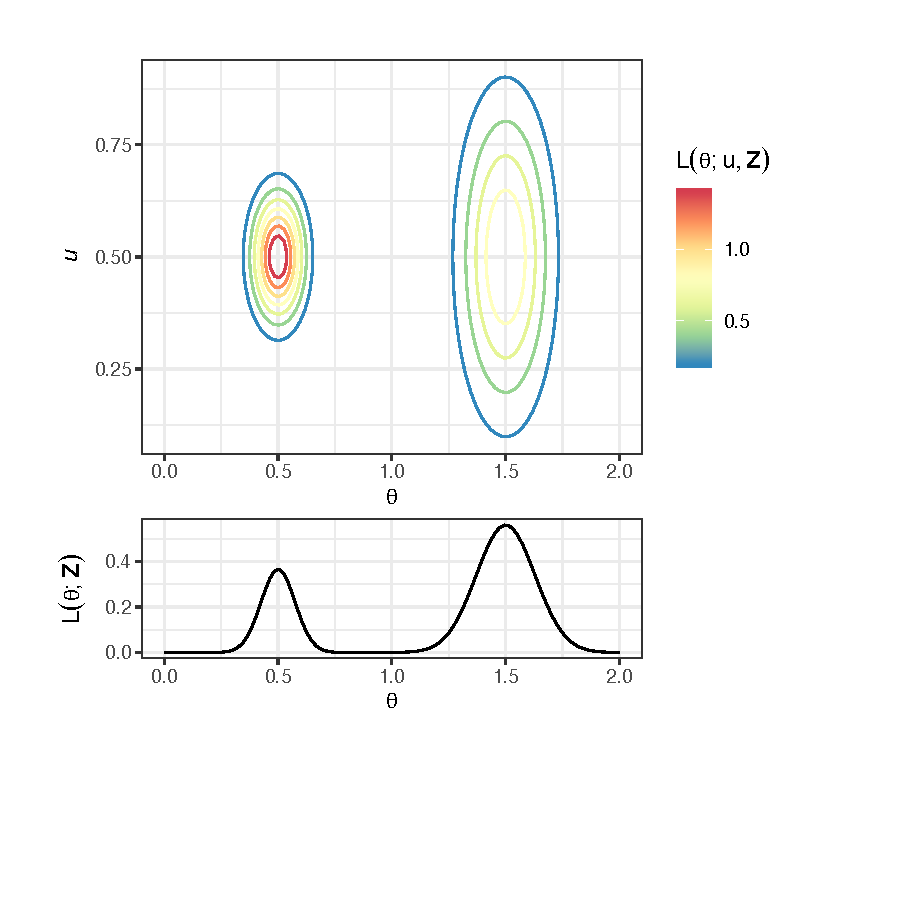
\includegraphics[width = 0.75\linewidth]{img/02-TwoProbMass.png}
%     \caption[Two regions of probability mass, demonstrating the different estimates of $\vec{\theta}$ which result from maximising the marginal and joint log-likelihood function]{Two regions of probability mass. The first, centred around $\theta = 0.5$, has a larger density than the second when $u$ is not marginalised out. However, the second, centred at $\theta = 1.5$, contributes more to the marginal likelihood $L(\theta; \vec{Z})$. Hence, an estimate of $\theta$ based on the marginal likelihood would yield $\hat{\theta} = 1.5$ and not $\hat{\theta} = 0.5$.}
%   \label{fig:02-04:TwoProbMass}
% \end{figure}



% \begin{figure}[t!]
%     \centering
%     \begin{subfigure}[b]{\linewidth}
%         \centering
%         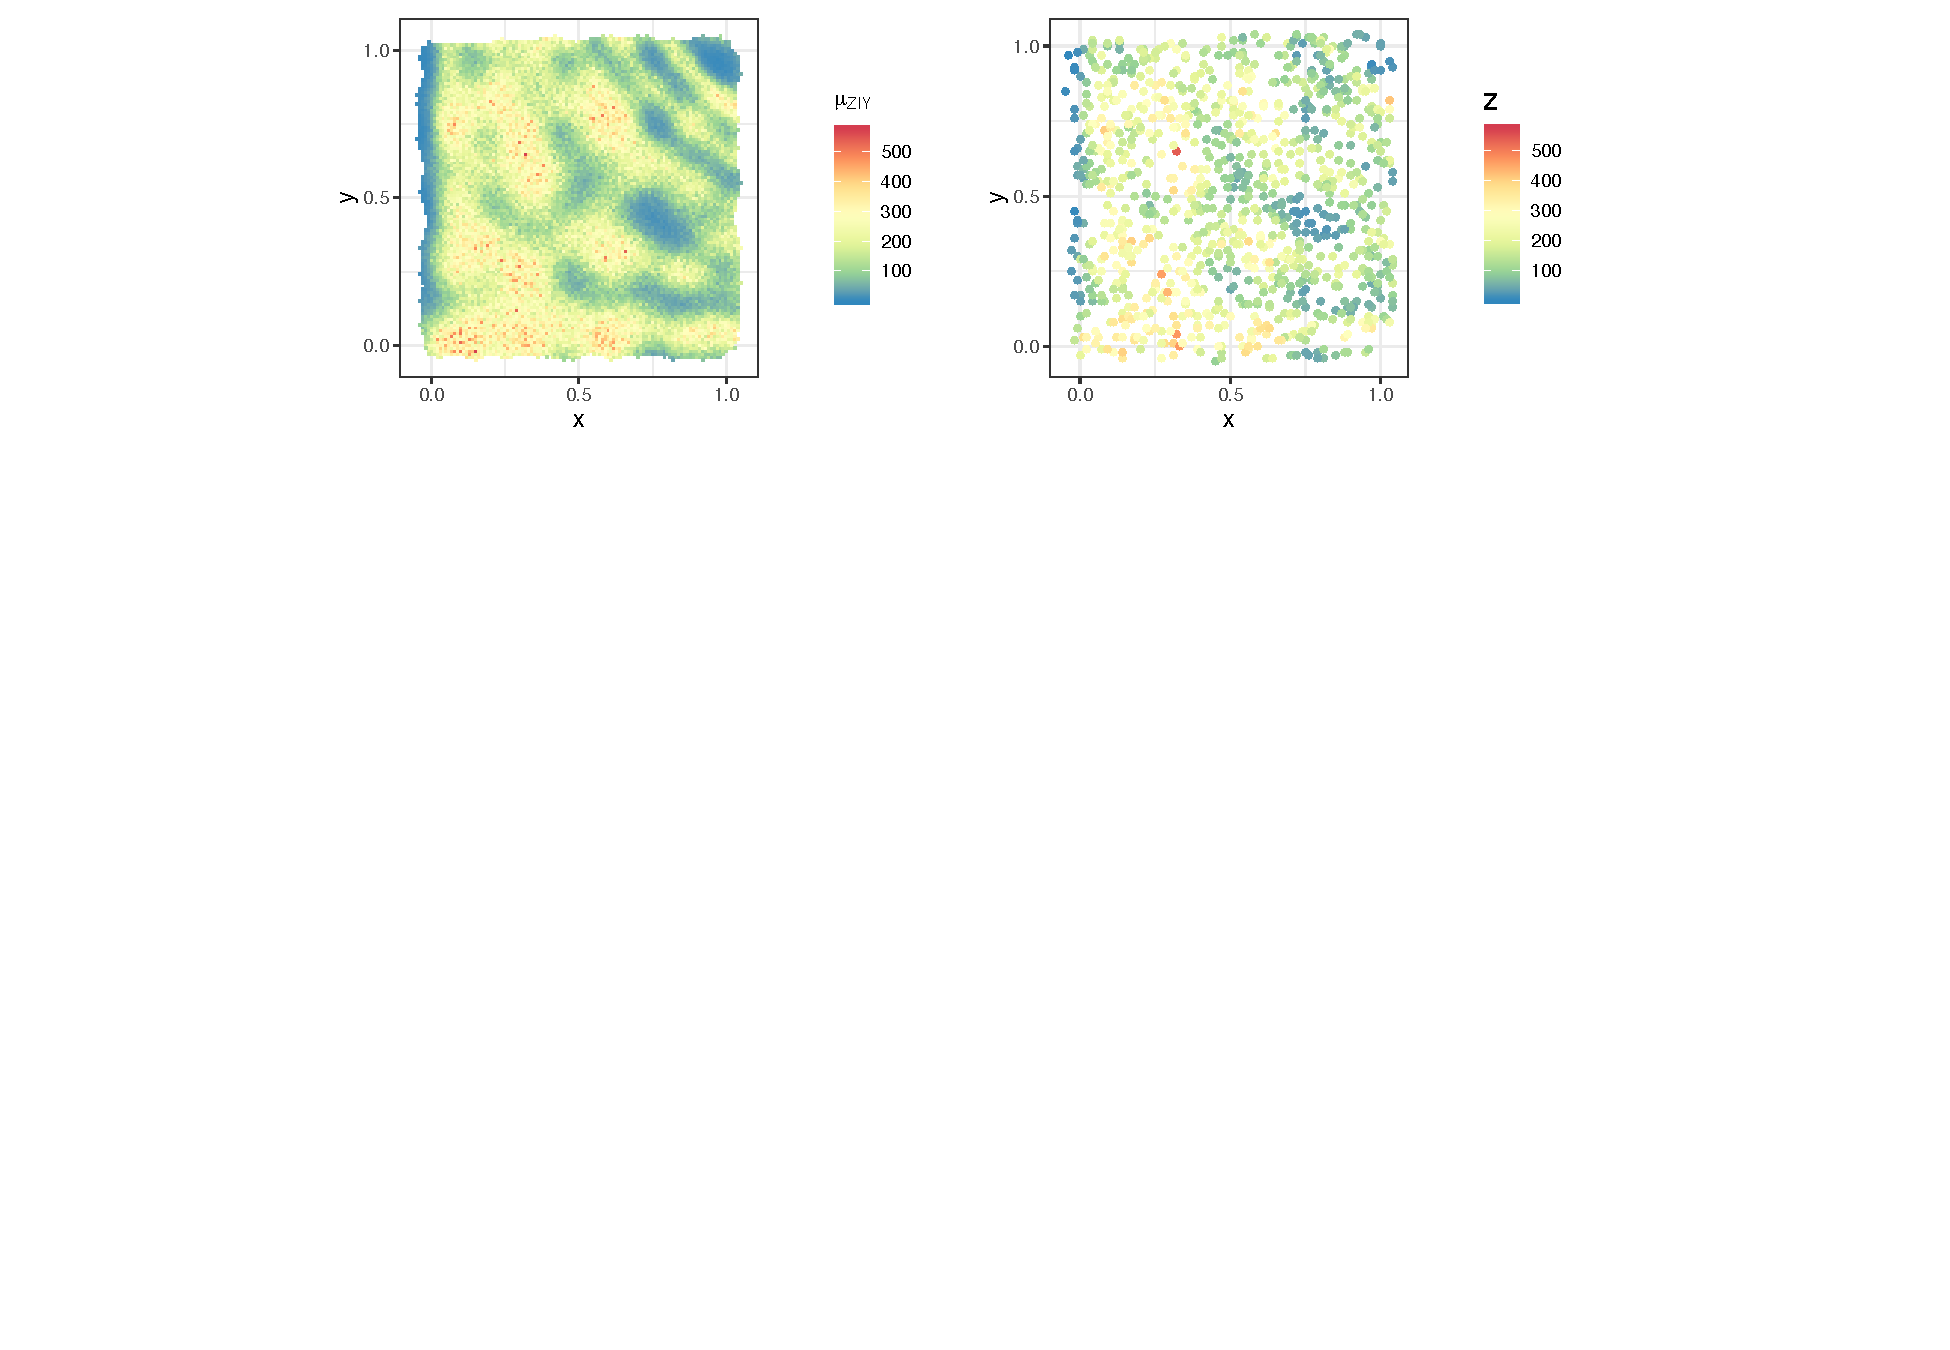
\includegraphics[width=\linewidth]{img/03-02-Poisson_plots2a.png}
%         \caption{(Left panel) True conditional mean of the data, $\mu(\cdot)$. (Right panel) Observed data.}\label{fig:03-02-PoissonResA}
%         \vspace{2\baselineskip}
%     \end{subfigure}
%     \begin{subfigure}[b]{\linewidth}
%         \centering
%         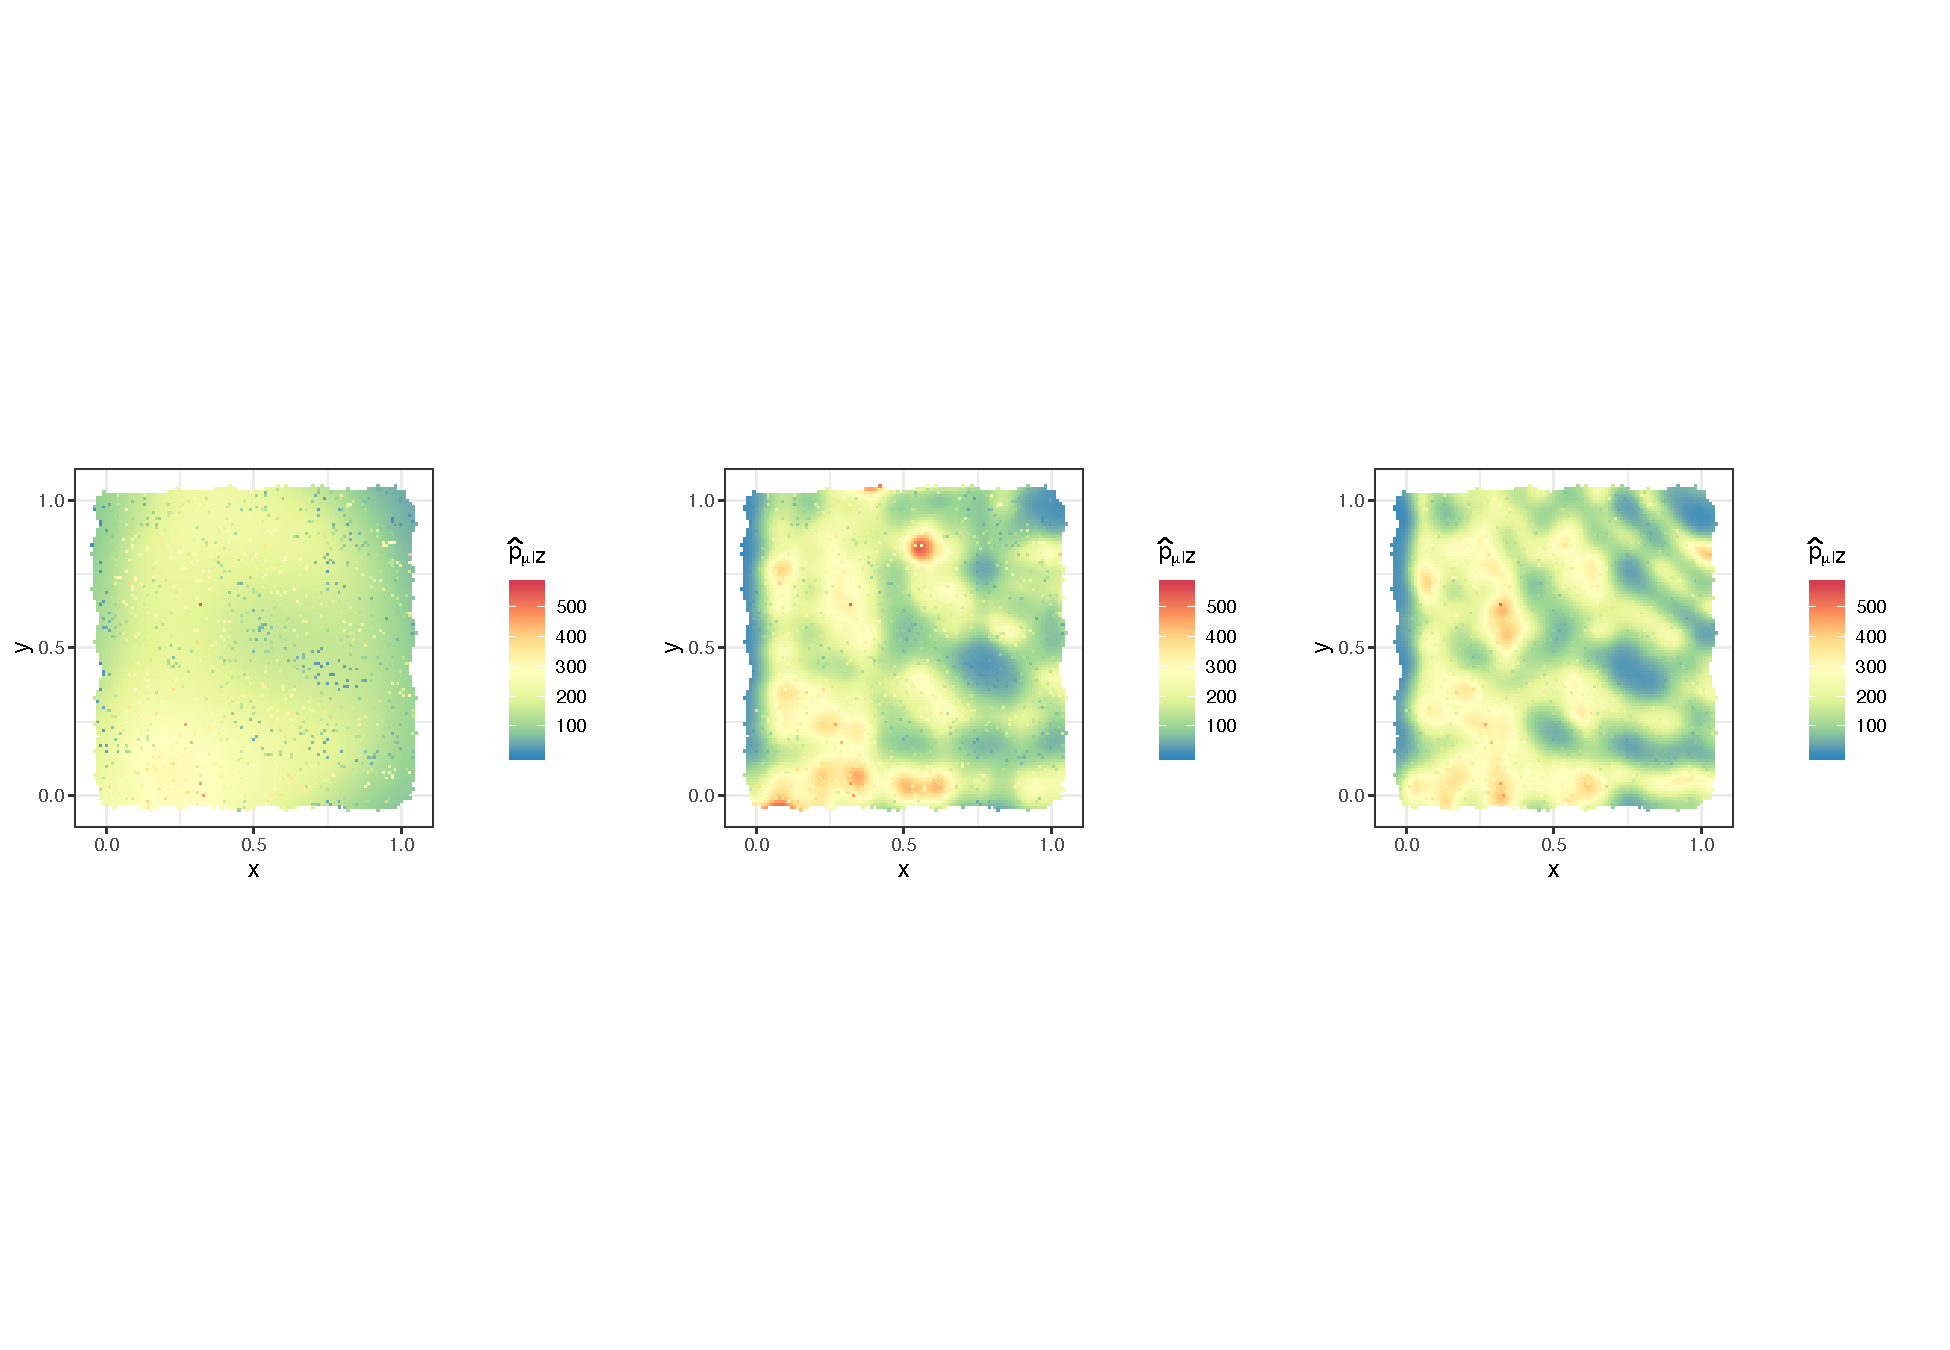
\includegraphics[width=\linewidth]{img/03-02-Poisson_plots2b.png}
%         \caption{Prediction maps using basis functions of one resolution (left panel), two resolutions (centre panel), and three resolutions (right panel).}\label{fig:03-02-PoissonResB}
%         \vspace{2\baselineskip}
%     \end{subfigure}
%         \begin{subfigure}[b]{\linewidth}
%         \centering
%         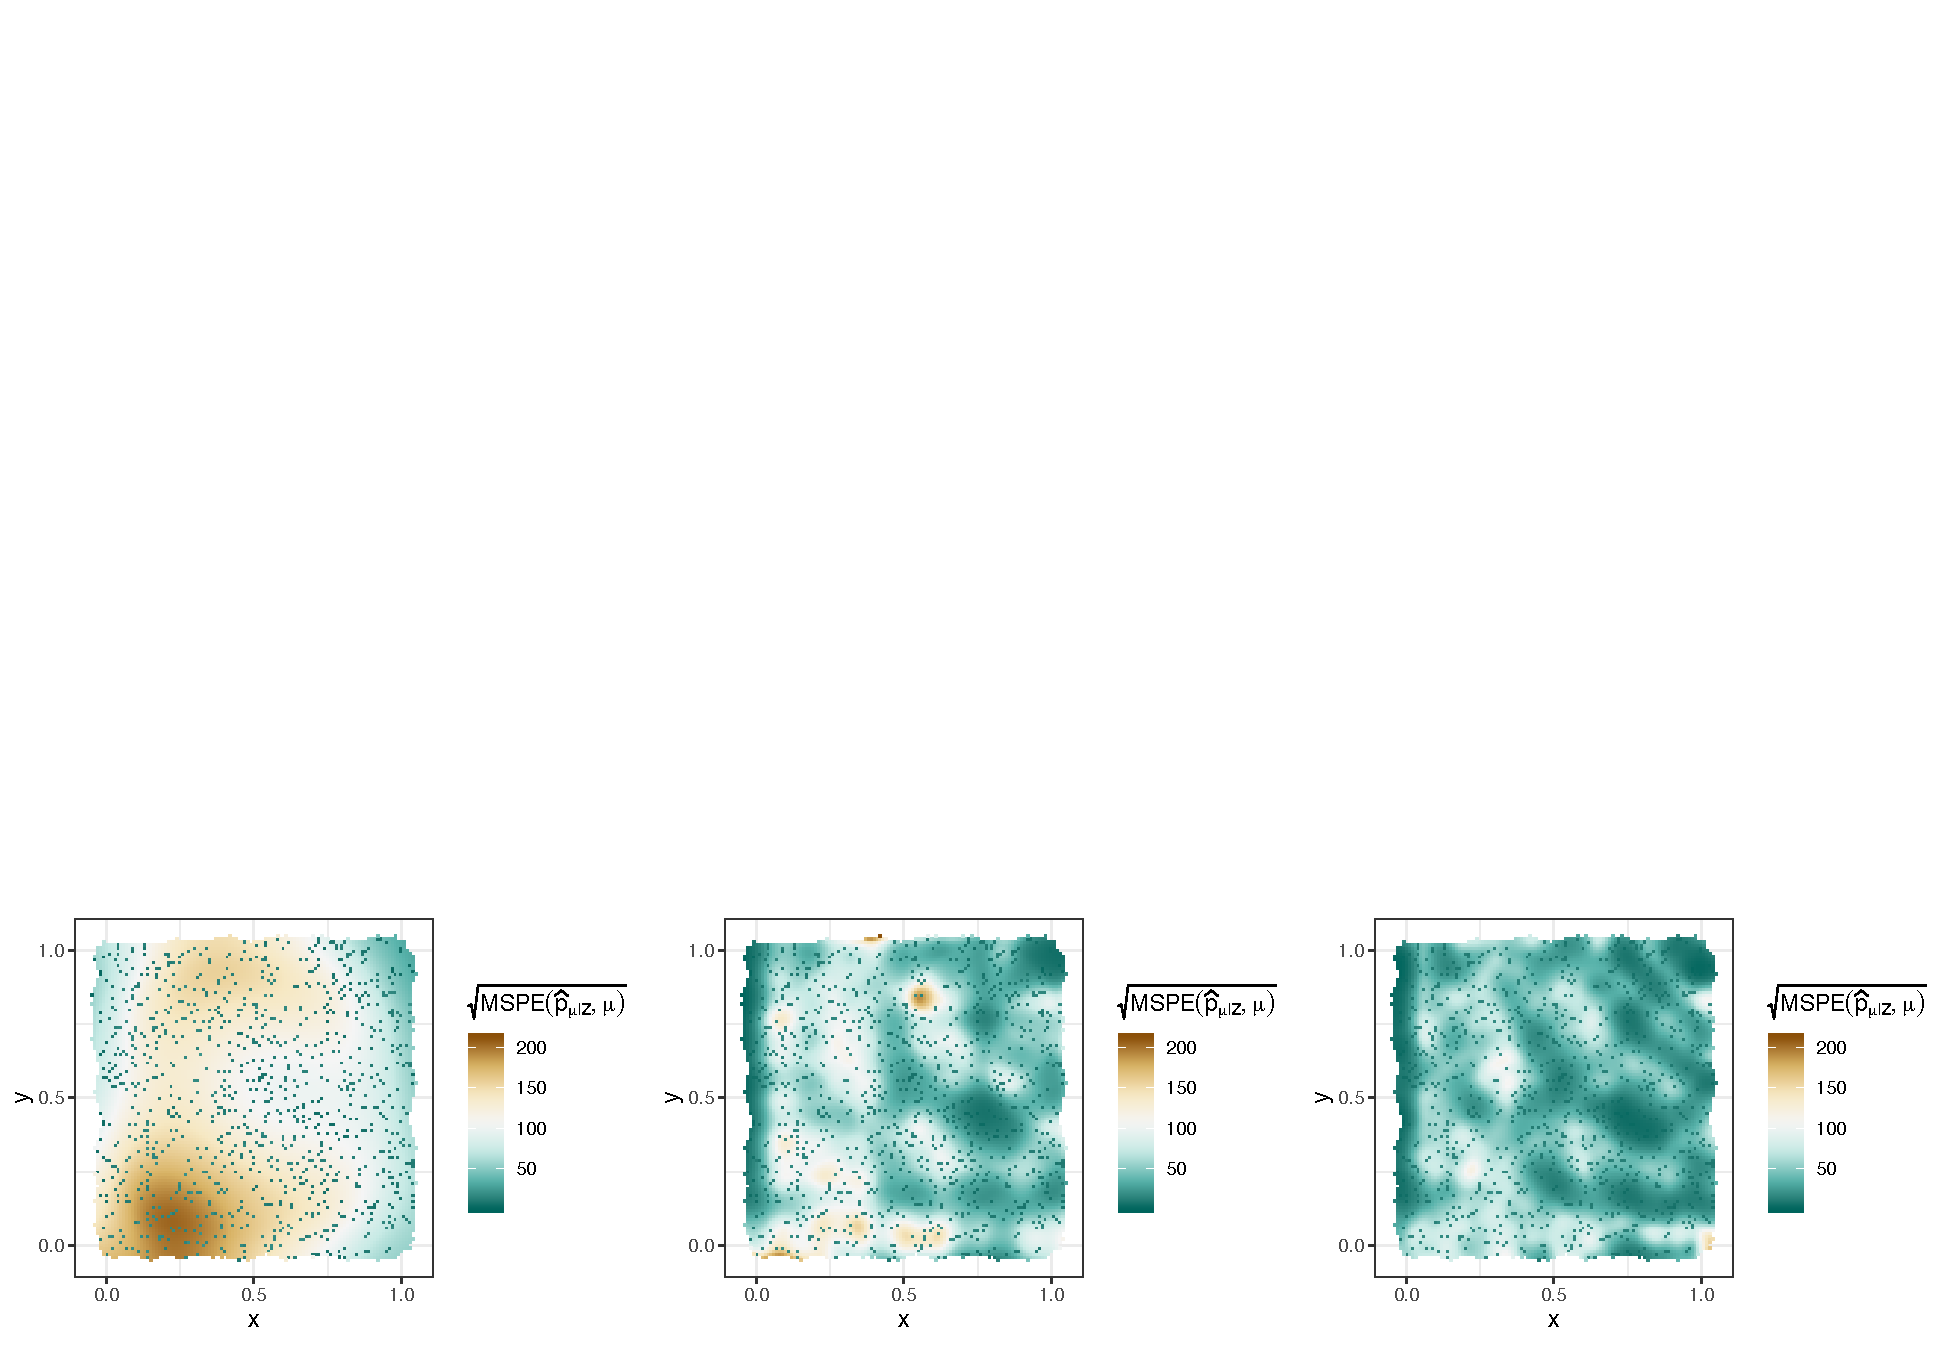
\includegraphics[width=\linewidth]{img/03-02-Poisson_plots2c.png}
%         \caption{Prediction uncertainty maps using basis functions of one resolution (left panel), two resolutions (centre panel), and three resolutions (right panel).}\label{fig:03-02-PoissonResC}
%         \vspace{2\baselineskip}
%     \end{subfigure}
%     \caption{\red{Use a common legend for each row if possible; probably use \code{facet\_wrap()} for the individual rows. We could reduce the size of the plot if we don't split into subfigures (i.e., have them as one big grid of plots). Perhaps we can omit this figure, or put it as an appendix.} Several panels summarising the analysis of a Poisson data set using one, two, and three resolutions of basis functions. Clearly, detail of our predictions increases with an increasing number of resolutions used; this is apparent by comparing the smooth, relatively uniform prediction and uncertainty maps created using one resolution, to the more intricate maps generated using three resolutions. The prediction uncertainty also decreases as we use more basis functions.}
%     \label{fig:03-02-PoissonRes}
% \end{figure}



%\begin{figure}[t!]
%    \centering
%    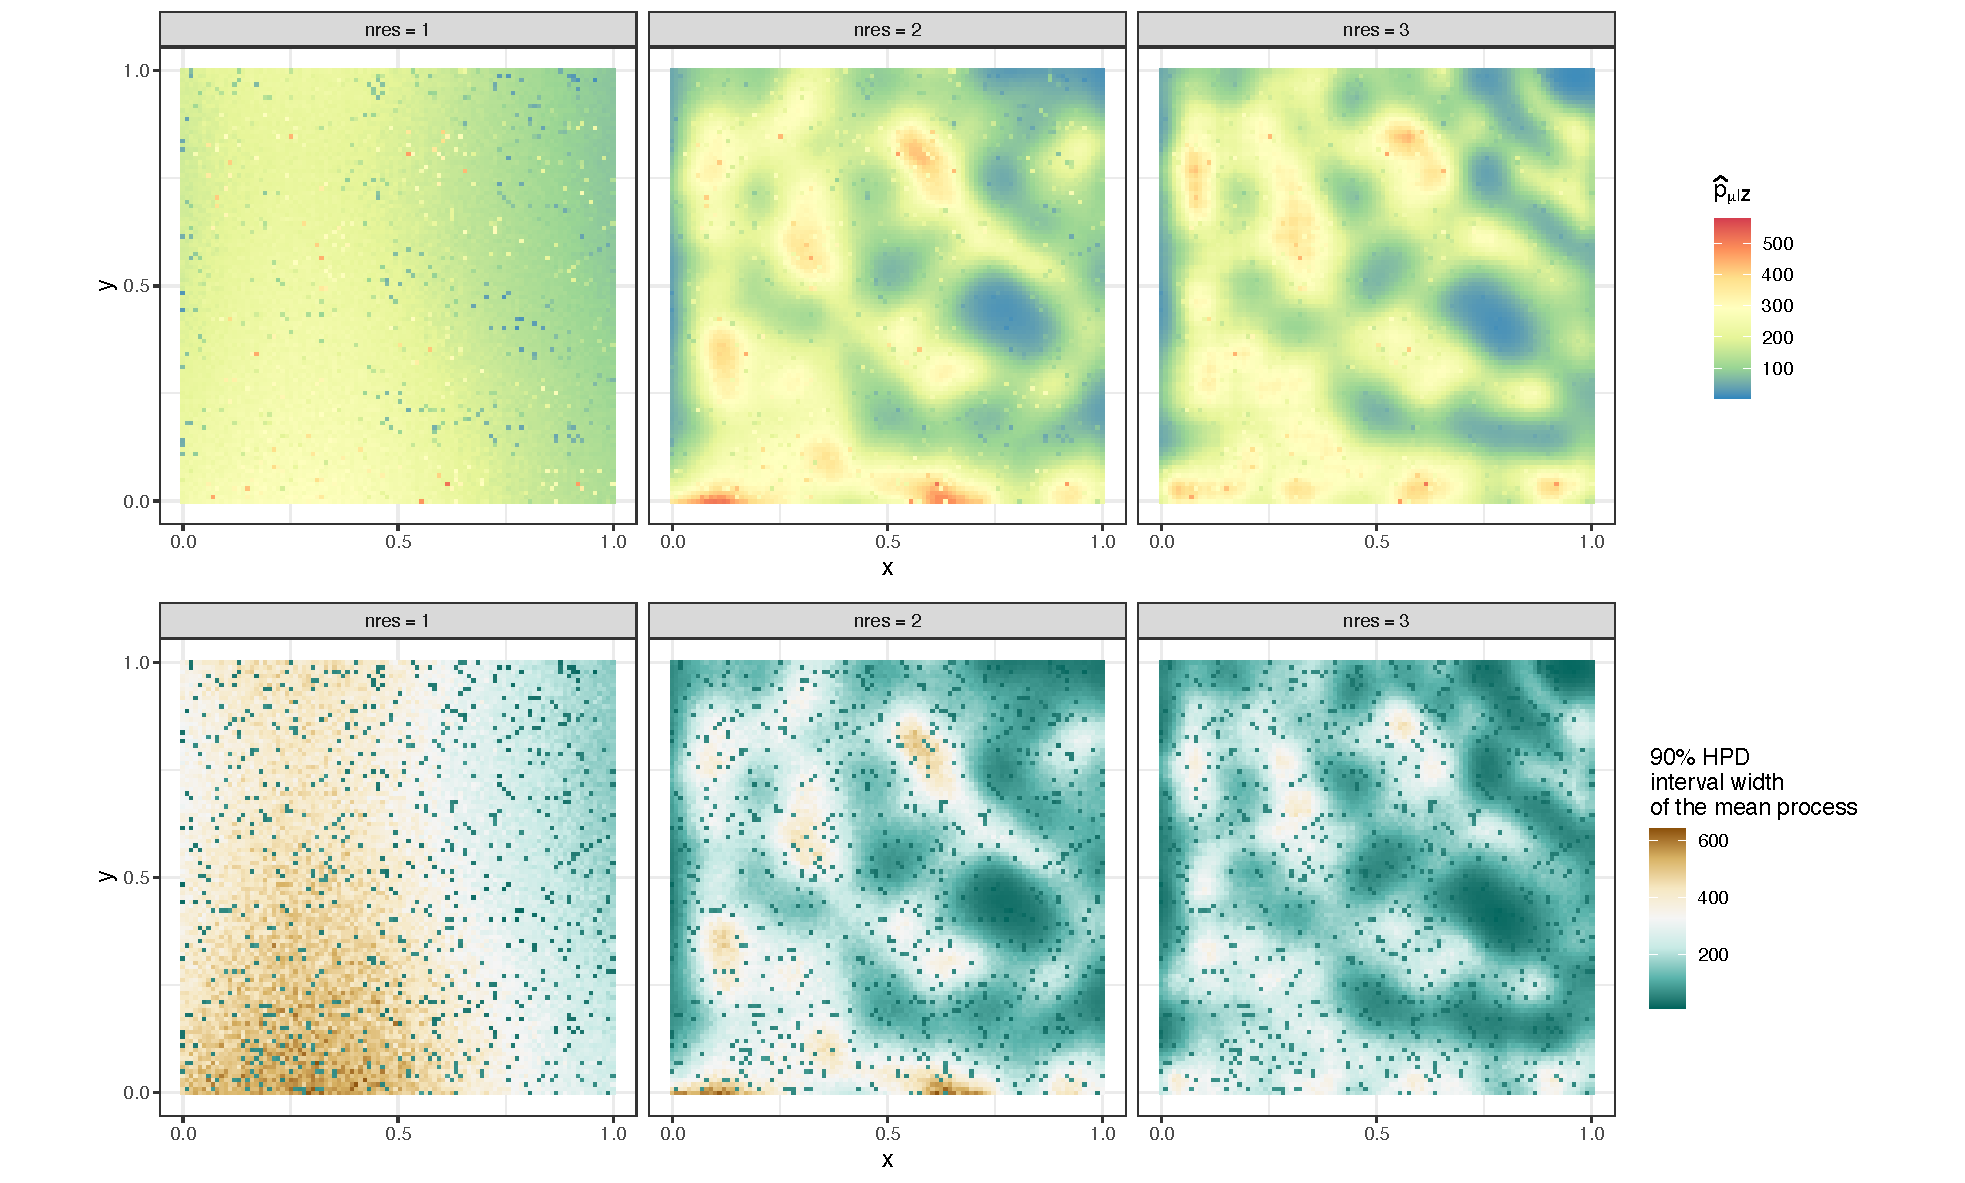
\includegraphics[width = \linewidth]{img/Poisson_multires.png}
%    \caption{Prediction and prediction uncertainty when analysing the Poisson data shown in Figure \ref{fig:Poisson_true_and_Z}. The first row corresponds to predictions of the mean process, $\mu(\cdot)$, while the second row corresponds to prediction uncertainty. The figure is divided into three columns, with the first, second, and third columns corresponding to predictions using one, two, and three resolutions of basis functions, respectively. 
%}   
%  \label{fig:Poisson_multires}
%\end{figure}


%\begin{figure}
%    \centering
%    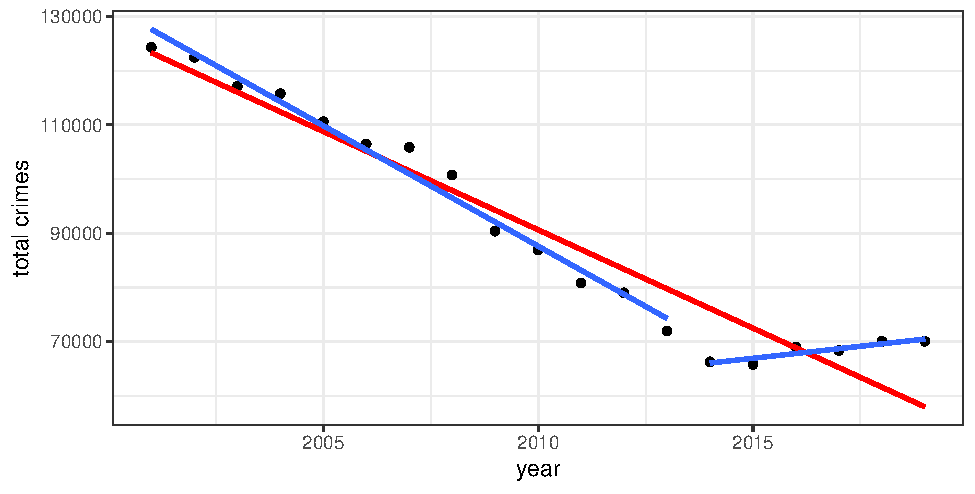
\includegraphics[width = 0.7\linewidth]{img/temporal_trend.png}
%    \caption{The total number of crimes committed across Chicago in each year, as well as two sets of fitted lines: the \red{red} line corresponds to a linear model that considers all data simultaneously, whilst the \textcolor{blue}{blue} line corresponds to a piecewise linear model split by the year 2014. The improved fit using a piecewise linear model suggests a piecewise temporal trend is appropriate for the Chicago analysis presented in Section \ref{sec:ST_example}.}   
%  \label{fig:chicago_temporal_trend}
%\end{figure}






%% Appendices

\newpage

\addtocontents{toc}{\protect\setcounter{tocdepth}{1}} % set only sections
\numberwithin{equation}{section}




\begin{appendix}


\section{Parametrisations of the basis-function coefficients}
\label{Appendix:CovarianceTapering}


%In this appendix, we provide details on the covariance tapering used to increase the sparsity of the prior variance matrix, $\vec{K}$, of the basis-function random coefficients. 
%Note that, for computational reasons, when \code{method = "TMB"} we typically recommend setting \code{K\_type = "precision"}, which flags the use of a sparse prior precision matrix, $\vec{Q}$, for the basis-function random coefficients. 
%
%
%Let $K_k(\vec{s}, \vec{s}^*)$ denote the covariance function of the random effects corresponding to the $k$th basis function resolution. 
% In \pkg{FRK}, we model $K_k(\vec{s}, \vec{s}^*)$ using the exponential covariance function,
%\begin{equation}\label{eqn:02-01:K_covariance_function}
%    K_k(\vec{s}, \vec{s}^*)  = \sigma^2_k \exp \left\{\frac{-d(\vec{s},\vec{s}^*)}{\tau_k}\right\}, 
%\end{equation}
%where $d(\vec{s},\vec{s}^*)$ is the distance between locations $\vec{s}, \vec{s}^* \in D$.  
% Given a covariance function we wish to taper, we must choose a taper function. 
% \citet{Furrer_2006_CovarianceTapering} recommend the Spherical taper for a Matérn covariance function with smoothness parameter $\nu\leq0.5$. 
% Noting that (\ref{eqn:02-01:K_covariance_function}) is special case of the Matérn covariance function with $\nu = 0.5$, we follow the recommendation of \cite{Furrer_2006_CovarianceTapering} and use the Spherical taper: 
%\begin{equation}\label{eqn:02-01:taper_function}
%K_{\beta_k}(\vec{s}, \vec{s}^*) 
%=
%\left\{1-\frac{d(\vec{s},\vec{s}^*)}{\beta_k}\right\}^2_{+}   \left\{1+\frac{d(\vec{s},\vec{s}^*)}{2\beta_k}\right\},
%\end{equation}
%where $x_{+} \equiv \max(0, x)$, and $\beta_k$ is a resolution-dependent tapering parameter controlling the strength of the taper. 
%The taper is zero for $d(\vec{s},\vec{s}^*) \geq \beta_k$, and one for $d(\vec{s},\vec{s}^*) = 0$. 
%The tapered covariance function for resolution $k$ is obtained by taking the product of the original covariance function (\ref{eqn:02-01:K_covariance_function}) and the taper function (\ref{eqn:02-01:taper_function}).%:
%%\[
%%{K_\textrm{tap}}_k(\vec{s}, \vec{s}^*)
%% =
%% K_k(\vec{s}, \vec{s}^*)K_{\beta_k}(\vec{s}, \vec{s}^*) 
%%%=
%%%\sigma^2_k \exp \left\{\frac{-d(\vec{s},\vec{s}^*)}{\tau_k}\right\}
%%%\left\{1-\frac{d(\vec{s},\vec{s}^*)}{\beta_k}\right\}^2_{+}   \left\{1+\frac{d(\vec{s},\vec{s}^*)}{2\beta_k}\right\}
%%,
%%\]
%%with the corresponding tapered variance-covariance matrix for resolution $k$ containing elements  
%%\[
%%    \{{\vec{K}_\textrm{tap}}_k\}_{i, j} 
%%    = 
%%    \sigma^2_k \exp \left\{\frac{-d(\vec{s}_{i, k},\vec{s}_{j, k})}{\tau_k}\right\}
%%    \left\{1-\frac{d(\vec{s}_{i, k},\vec{s}_{j, k})}{\beta_k}\right\}^2_{+}   \left\{1+\frac{d(\vec{s}_{i, k},\vec{s}_{j, k})}{2\beta_k}\right\}.
%%\]
%%Finally, the full tapered variance-covariance matrix for the basis-function random effects $\vec{\eta}$ is thus
%%\[
%%\vec{K}_\textrm{tap} = 
%%\begin{pmatrix}
%%{\vec{K}_\textrm{tap}}_1   &           &           \\ 
%%            & \ddots    &           \\
%%            &           & {\vec{K}_\textrm{tap}}_l
%%\end{pmatrix}.
%%\]
%
%
%
%To use this method of covariance-tapering we must specify the taper parameter $\beta_k$ for each resolution. 
%% We first note that the basis functions created by \pkg{FRK} are constructed in a regular grid, whereby each resolution has $3^2=9$ times as many functions as the preceding resolution. 
%% Hence, the effective range of three basis functions at resolution $k$ is equal to the effective range of a single basis function at resolution $k-1$. 
%% We argue heuristically that basis functions at the $k$th resolution should not be used to capture scales that extend beyond a few ranges of the basis functions at the $(k-1)$th resolution. 
%We do so based on the minimum distance between basis functions at the given resolution. Specifically, we set the tapering parameter of resolution $k$ to be $\beta_k = \texttt{taper} \times \text{mindist}(k)$, where $\text{mindist}(k)$ is the minimum distance between the centroids of basis functions at the $k$th resolution and \code{taper} is an argument set by the user which determines the strength of the covariance tapering. 
%Decreasing $\beta_k$ will increase the sparsity of 
%the tapered covariance matrix, %${\vec{K}_\textrm{tap}}_k$, 
% whilst increasing $\beta_k$ will decrease 
% %the sparsity of ${\vec{K}_\textrm{tap}}_k$.
% its sparsity.  
%  Taking $\beta_k$ to infinity will recover the full block exponential covariance formulation.% of $\vec{K}_k$.
%
%%Covariance tapering is done for computational reasons. In particular, the derivations and results in this work do not depend on whether the matrices $\vec{K}$ or $\vec{K}_\textrm{tap}$ are used. Hence, for notational convenience, we do not make a distinction between $\vec{K}$ and $\vec{K}_\textrm{tap}$.  


Recall from Section \ref{subsection:04-01:ProcessLayer} that \pkg{FRK} v2 allows the basis-function coefficients, $\vec{\eta}$, to be parametrised using either a prior covariance matrix, $\vec{K}$, or using a prior precision matrix, $\vec{Q}$.  
 In this appendix, we describe these matrices.
 Recall that both formulations use block-diagonal matrices, wherein basis-function coefficients are independent of the basis-function coefficients in differing resolutions. Hence, we need only describe the intra-resolution dependencies.
 
\subsection{Covariance matrix}

% First, we describe $\vec{K}$. 
 Let $K_k(\vec{s}, \vec{s}^*)$ denote the covariance function of the basis-function coefficients corresponding to the $k$th basis function resolution. 
 In \pkg{FRK}, we model $K_k(\vec{s}, \vec{s}^*)$ using the exponential covariance function,
\begin{equation}\label{eqn:02-01:K_covariance_function}
    K_k(\vec{s}, \vec{s}^*)  = \sigma^2_k \exp \left\{\frac{-d(\vec{s},\vec{s}^*)}{\tau_k}\right\}, 
\end{equation}
where $d(\vec{s},\vec{s}^*)$ is the distance between locations $\vec{s}, \vec{s}^* \in D$.  
Clearly (\ref{eqn:02-01:K_covariance_function}) is always non-zero for $\sigma^2_k > 0$, however 
 it is often reasonable to assume that coefficients associated with fine-resolution basis functions separated by medium-to-large distances are uncorrelated. 
To increase sparsity, \pkg{FRK} v2 allows covariance tapering \citep{Furrer_2006_CovarianceTapering} of the intra-resolution covariance function. %, so that, if the distance between given basis functions is sufficiently large, the covariance of the coefficients is tapered to zero. 
% Given a covariance function we wish to taper, we must choose a taper function. 
% \citet{Furrer_2006_CovarianceTapering} recommend the Spherical taper for a Matérn covariance function with smoothness parameter $\nu\leq0.5$. 
 Noting that (\ref{eqn:02-01:K_covariance_function}) is a special case of the Matérn covariance function with $\nu = 0.5$, we follow the recommendation of \cite{Furrer_2006_CovarianceTapering} and use the Spherical taper: 
\begin{equation}\label{eqn:02-01:taper_function}
%K_{\beta_k}(\vec{s}, \vec{s}^*) 
T_{\beta_k}(\vec{s}, \vec{s}^*) 
=
\left\{1-\frac{d(\vec{s},\vec{s}^*)}{\beta_k}\right\}^2_{+}   \left\{1+\frac{d(\vec{s},\vec{s}^*)}{2\beta_k}\right\},
\end{equation}
where $x_{+} \equiv \max(0, x)$, and $\beta_k$ is a resolution-dependent tapering parameter controlling the strength of the taper. 
%The taper is zero for $d(\vec{s},\vec{s}^*) \geq \beta_k$, and one for $d(\vec{s},\vec{s}^*) = 0$. 
In \pkg{FRK} v2, we define $\beta_k$ based on the minimum distance between basis-function centroids; specifically, we set $\beta_k = \texttt{taper} \times \text{mindist}(k)$, where $\text{mindist}(k)$ is the minimum distance between the centroids of basis functions at the $k$th resolution and \code{taper} is a user-specified argument.
%Decreasing $\beta_k$ will increase the sparsity of 
%the tapered covariance matrix, %${\vec{K}_\textrm{tap}}_k$, 
% whilst increasing $\beta_k$ will decrease 
% %the sparsity of ${\vec{K}_\textrm{tap}}_k$.
% its sparsity.  
%  Taking $\beta_k$ to infinity will recover the full block exponential covariance formulation.% of $\vec{K}_k$.
The tapered covariance function is obtained by taking the product of the original covariance function (\ref{eqn:02-01:K_covariance_function}) and the taper function (\ref{eqn:02-01:taper_function}).%:
%\[
%{K_\textrm{tap}}_k(\vec{s}, \vec{s}^*)
% =
% K_k(\vec{s}, \vec{s}^*)K_{\beta_k}(\vec{s}, \vec{s}^*) 
%%=
%%\sigma^2_k \exp \left\{\frac{-d(\vec{s},\vec{s}^*)}{\tau_k}\right\}
%%\left\{1-\frac{d(\vec{s},\vec{s}^*)}{\beta_k}\right\}^2_{+}   \left\{1+\frac{d(\vec{s},\vec{s}^*)}{2\beta_k}\right\}
%,
%\]
%with the corresponding tapered variance-covariance matrix for resolution $k$ containing elements  
%\[
%    \{{\vec{K}_\textrm{tap}}_k\}_{i, j} 
%    = 
%    \sigma^2_k \exp \left\{\frac{-d(\vec{s}_{i, k},\vec{s}_{j, k})}{\tau_k}\right\}
%    \left\{1-\frac{d(\vec{s}_{i, k},\vec{s}_{j, k})}{\beta_k}\right\}^2_{+}   \left\{1+\frac{d(\vec{s}_{i, k},\vec{s}_{j, k})}{2\beta_k}\right\}.
%\]
%Finally, the full tapered variance-covariance matrix for the basis-function random effects $\vec{\eta}$ is thus
%\[
%\vec{K}_\textrm{tap} = 
%\begin{pmatrix}
%{\vec{K}_\textrm{tap}}_1   &           &           \\ 
%            & \ddots    &           \\
%            &           & {\vec{K}_\textrm{tap}}_l
%\end{pmatrix}.
%\]



%To use this method of covariance-tapering we must specify the taper parameter $\beta_k$ for each resolution. 
%% We first note that the basis functions created by \pkg{FRK} are constructed in a regular grid, whereby each resolution has $3^2=9$ times as many functions as the preceding resolution. 
%% Hence, the effective range of three basis functions at resolution $k$ is equal to the effective range of a single basis function at resolution $k-1$. 
%% We argue heuristically that basis functions at the $k$th resolution should not be used to capture scales that extend beyond a few ranges of the basis functions at the $(k-1)$th resolution. 
%We do so based on the minimum distance between basis functions at the given resolution. Specifically, we set the tapering parameter of resolution $k$ to be $\beta_k = \texttt{taper} \times \text{mindist}(k)$, where $\text{mindist}(k)$ is the minimum distance between the centroids of basis functions at the $k$th resolution and \code{taper} is a user-specified argument.
%Decreasing $\beta_k$ will increase the sparsity of 
%the tapered covariance matrix, %${\vec{K}_\textrm{tap}}_k$, 
% whilst increasing $\beta_k$ will decrease 
% %the sparsity of ${\vec{K}_\textrm{tap}}_k$.
% its sparsity.  
%  Taking $\beta_k$ to infinity will recover the full block exponential covariance formulation.% of $\vec{K}_k$.

%Covariance tapering is done for computational reasons. In particular, the derivations and results in this work do not depend on whether the matrices $\vec{K}$ or $\vec{K}_\textrm{tap}$ are used. Hence, for notational convenience, we do not make a distinction between $\vec{K}$ and $\vec{K}_\textrm{tap}$.  


%The covariance matrix $\vec{K}$ is block-diagonal, wherein basis-function coefficients \textit{between} resolutions are independent, and basis-function coefficients \textit{within} a resolution have a correlation that decays exponentially with the distance between basis-function centroids. 
%When the prior covariance matrix is used to model dependence between elements of $\vec{\eta}$, $\vec{K}$ is block-diagonal, wherein basis-function coefficients \textit{between} resolutions are independent, whilst basis-function coefficients \textit{within} a resolution are correlated, with the correlation decaying exponentially with the distance between basis function centroids. 
% This leads to a block-diagonal form for $\vec{K}$, that is, 
% \[
% \vec{K} = 
% \begin{pmatrix}
% \vec{K}_1   &           &           \\ 
%             & \ddots    &           \\
%             &           & \vec{K}_{l}
% \end{pmatrix},
% \]
% where $l$ is the number of basis function resolutions, and 
%The covariance between the $i$th and $j$th basis function of resolution $k$ is
%\[
%    \{\vec{K}_k\}_{i, j} = \sigma^2_k \exp \left\{\frac{-d(\vec{s}_{i, k},\vec{s}_{j, k})}{\tau_k}\right\},
%\]
%where $d(\vec{s},\vec{s}^*) \equiv \norm{\vec{s} - \vec{s}^*}$ is the Euclidean distance between two locations $\vec{s},\vec{s}^* \in D$, and the parameters $\sigma^2_k$ and $\tau_k$ are variance components pertaining to resolution $k$. 
%The exponential decay implies 
%The intra-resolution covariance function is always non-zero; however
%%, after parameter estimation, 
% it is common to observe that coefficients associated with basis functions separated by medium-to-large distances have almost zero correlation. 
%To increase sparsity in $\vec{K}$, \pkg{FRK} v2 allows covariance tapering \citep{Furrer_2006_CovarianceTapering} of the intra-resolution covariances %, so that, if the distance between given basis functions is sufficiently large, the covariance of the coefficients is tapered to zero. 
%(see Appendix \ref{Appendix:CovarianceTapering}).


\subsection{Precision matrix}

\pkg{FRK} v2 offers two types of sparse precision matrices: One for regularly spaced basis functions, and another for irregularly spaced basis functions. 
 This choice is determined by the field \code{regular} in the \class{Basis} object.

When the basis functions are regularly spaced (\code{regular = TRUE}), \pkg{FRK} v2 uses a precision matrix that is related to that used in the \proglang{R} package \pkg{LatticeKrig} \citep{Nychka_2016_LatticeKrig}. 
 Let $\mathcal{N}_{i, k}$ denote the set of first-order horizontal and vertical neighbouring basis functions of the $i$th basis function of resolution $k$, 
%The number of elements in $\mathcal{N}_{i, k}$, $|\mathcal{N}_{i, k}|$, will be four for interior basis functions, three for basis functions on edges, and two for basis functions on corners when the basis functions are arranged on a regular grid in $\mathbb{R}^2$.
 and let $\vec{Q}_k$ denote the prior precision matrix of the basis-function coefficients at resolution $k$. 

We model the elements of $\vec{Q}_k$ as
\begin{equation}\label{eqn:Q_k}
    \{\vec{Q}_{k}\}_{i, j}
=
\begin{cases}
\kappa_k + \rho_k |\mathcal{N}_{i, k}|   & i = j\\
-\rho_k & j \in \mathcal{N}_{i, k} \\
0 & \text{otherwise}
\end{cases},
\end{equation}
where $\kappa_k$ and $\rho_k$ are parameters that need to be estimated. 
%The full precision matrix $\vec{Q}$ is then $\text{bdiag}(\{\vec{Q}_k: k = 1,...,l\})$, where $l$ is the number of basis-function resolutions, and $\text{bdiag}(\cdot)$ returns a block-diagonal matrix from its arguments. 
We note that $\vec{Q}_k$ is diagonally dominant, and hence it is positive definite. 
 This formulation implies that the coefficient of a given basis-function is conditionally independent of all other basis-function coefficients given the coefficients of its first-order vertical and horizontal neighbours. 
 We also note that \pkg{LatticeKrig} uses $\vec{Q}_k^\tp\vec{Q}_k$ as the precision matrix blocks. 


 To cater for irregularly spaced basis functions, \pkg{FRK} v2 also offers a sparse precision matrix which considers the distance between basis functions:  
% In this setting, we model the elements of $\vec{Q}_k$ as
\begin{equation}\label{eqn:K_type_precision-block-exponential}
\{\vec{Q}_{k}\}_{i, j}
=
%\begin{cases}
%\delta_k -\sum_{j \neq i}\{\vec{Q}_{k}\}_{i, j}  & i = j\\
%-\rho_k \exp \left\{\frac{-d(\vec{s}_{i, k}, \vec{s}_{j, k})}{\tau_k}\right\}
%    \left\{1-\frac{d(\vec{s}_{i, k}, \vec{s}_{j, k})}{\beta_k}\right\}^2_{+}   \left\{1+\frac{d(\vec{s}_{i, k}, \vec{s}_{j, k})}{2\beta_k}\right\} & i \neq j\\
%\end{cases},
\begin{cases}
\kappa_k -\sum_{j \neq i}\{\vec{Q}_{k}\}_{i, j}  & i = j\\
-\rho_k \exp \left\{\frac{-d(\vec{s}_{i, k}, \vec{s}_{j, k})}{\tau_k}\right\}
    T_{\beta_k}(\vec{s}_{i, k}, \vec{s}_{j, k})  & i \neq j\\
\end{cases},
\end{equation}
where $\kappa_k$, $\rho_k$, and $\kappa_k$ are parameters that need to be estimated, and $T_{\beta_k}(\cdot, \cdot)$ is defined as in the preceding section. 
 Again, this matrix is diagonally dominant, and hence positive definite. 
 Equation (\ref{eqn:K_type_precision-block-exponential}) is in some ways a generalisation of (\ref{eqn:Q_k}).
 This formulation implies that the partial correlation between basis-function coefficients decays exponentially with distance until a point (controlled by the tapering parameter $\beta_k$) at which the basis-function coefficients are conditionally independent. 

%For notational convenience, we use $\vec{\vartheta}$ to denote the parameters associated with either $\vec{K}$ or $\vec{Q}$. 






%\section{Prediction}\label{app:prediction}
%
%\numberwithin{equation}{subsection}
%
%
%In this appendix, we provide details for how we predict the latent process $Y(\cdot)$, the mean process $\mu(\cdot)$, and the noisy data process. 
%%For simplicity, we provide details for the simple kriging case, whereby the fixed-effects $\vec{\alpha}$ are assumed to be known quantities, with the uncertainty of their estimation unaccounted for.
%%The universal kriging case, which, in this framework, involves treating $\vec{\alpha}$ as random quantities, is a straightforward extension. 
%For notational convenience, we treat the regression parameters, $\vec{\alpha}$, as known.
%
%
%\subsection{Prediction of the latent process}\label{sec:04-03-01:YProcessPrediction}
%
%
%The predictor of $Y_i$, the latent process $Y(\cdot)$ evaluated over the BAU $A_i$, is the expectation of $Y_i$ conditional on the data, parameters, and fixed effects;
%\begin{equation}\label{eqn:02-03:pYgivenZ}
%    \pYgivenZ{A_i}
%    \equiv
%    \ECurly{Y_i \mid \vec{Z}, \vec{\theta}}.
%\end{equation}
%Recall from Section 
%%\ref{sec:marginal_likelihood} 
%\ref{subsection:02-03:Estimation} 
% that the posterior distribution of the random effects, $\vec{u} \equiv (\vec{\eta}^\tp, \vec{\xi}^\tp)^\tp$, is approximated to be Gaussian (as we use the Laplace approximation), and hence the posterior distribution of $Y_i$ is also approximated to be Gaussian.
%Therefore, another quantity of interest is the posterior variance;
%\begin{equation}\label{eqn:02-03:varYgivenZ}
%    \varCurly{Y_i \mid \vec{Z}, \vec{\theta}}.
%\end{equation}
%Given estimates of the posterior expectation and precision matrix of $\vec{u}$ using \pkg{TMB}, we can compute (\ref{eqn:02-03:pYgivenZ}) and (\ref{eqn:02-03:varYgivenZ}) in at least two ways. 
% The first is an analytic approach using basic expectation and variance properties, and the second is via Monte Carlo simulation.
%
%
%
%\subsubsection{Analytic approach}
%
%%Recall that for a location $\vec{s}\in D$, the process layer, irrespective of the assumed distribution of the data, is given by
%%\[
%%Y(\vec{s}) = \vec{t}(\vec{s})^\tp\vec{\alpha} + \phi(\vec{s})^\tp \vec{\eta} + \xi(\vec{s}); \quad \vec{s} \in D.
%%\]
%%Forms for the posterior expectation and variance can be derived straightforwardly. 
%% However, before doing so, we explore a fact that will simplify some terms considerably. 
%
%Recall that the process layer, irrespective of the assumed distribution of the data, is given by (\ref{eqn:04-01:Y(s)}). Defining $\vec{\xi}_O$ and $\vec{\xi}_U$ as the elements of $\vec{\xi}$ associated with observed and unobserved BAUs, respectively, it can be shown \citep[e.g.,][]{Sengupta_Cressie_2013_spatial_GLMM_FRK} that $\vec{\xi}_U$ are conditionally independent of all other random quantities in the model; that is, $[\vec{\xi}_U \mid \vec{Z}, \vec{\eta}, \vec{\xi}_O, \vec{\theta}] = [\vec{\xi}_U \mid \sigma^2_\xi]$. 
%%Define $\vec{\xi}_O$ and $\vec{\xi}_U$ as the elements of $\vec{\xi}$ associated with observed and unobserved BAUs, respectively.
%%\cite{Sengupta_Cressie_2013_spatial_GLMM_FRK} showed that, under the framework of a spatial GLMM with a spatial mixed effects model for the process layer, and assuming the fine-scale variation terms $\vec{\xi}$ are independent a priori, the unobserved fine-scale variation terms, $\vec{\xi}_U$, are conditionally independent of all other random quantities in the model; that is, that $[\vec{\xi}_U \mid \vec{Z}, \vec{\eta}, \vec{\xi}_O, \vec{\theta}] = [\vec{\xi}_U \mid \sigma^2_\xi]$.
%%This allows for considerable simplification of the posterior expectation and variance at unobserved locations. 
%%Specifically, (\ref{eqn:02-03:pYgivenZ}) becomes 
%Then, the posterior expectation (\ref{eqn:02-03:pYgivenZ}) is 
%\begin{align*}
%    \pYgivenZ{A_i}
%    &=
%    \ECurly{Y_i \mid \vec{Z}, \vec{\theta}}\\
%    &=
%    \vec{t}(A_i)^\tp\vec{\alpha} + \vec{\phi}(A_i)^\tp \E{\vec{\eta} \mid \vec{Z}, \vec{\theta}} + \ECurly{\xi_i \mid \vec{Z}, \sigma^2_\xi}\\
%    &=
%    \begin{cases} 
%      \vec{t}(A_i)^\tp\vec{\alpha} + \vec{\phi}(A_i)^\tp \E{\vec{\eta} \mid \vec{Z}, \vec{\theta}} + \ECurly{\xi_i \mid \vec{Z}, \sigma^2_\xi} & A_i\in D^O \\
%      \vec{t}(A_i)^\tp\vec{\alpha} + \vec{\phi}(A_i)^\tp \E{\vec{\eta} \mid \vec{Z}, \vec{\theta}} & A_i\notin D^O
%   \end{cases},
%\end{align*}
%where recall that $D^O$ denotes the set of observations supports. 
% The posterior variance (\ref{eqn:02-03:varYgivenZ}) is 
%\begin{align*}
%    &\varCurly{Y_i \mid \vec{Z}, \vec{\theta}} \nonumber \\
%    &=
%    \varCurly{\vec{\phi}(A_i)^\tp \vec{\eta} \mid \vec{Z}, \vec{\theta}}
%    +
%    \varCurly{\xi_i \mid \vec{Z}, \sigma^2_\xi}
%    +
%    2 \covCurlyConditional{ \vec{\phi}(A_i)^\tp\vec{\eta}}{\xi_i }{ \vec{Z}, \vec{\theta} } \nonumber \\
%    &=
%    \vec{\phi}(A_i)^\tp\vec{\Sigma}_{\vec{\eta} \mid \vec{Z}}\vec{\phi}(A_i)
%    +
%    \varCurly{\xi_i \mid \vec{Z}, \sigma^2_\xi}
%    +
%    2\vec{\phi}(A_i)^\tp
%     \covCurlyConditional{ \vec{\eta} }{\xi_i }{\vec{Z}, \vec{\theta}} \nonumber \\
%    &=
%    \begin{cases}
%    \vec{\phi}(A_i)^\tp\vec{\Sigma}_{\vec{\eta} \mid \vec{Z}}\vec{\phi}(A_i)
%    +
%    \varCurly{\xi_i \mid \vec{Z}, \sigma^2_\xi}
%    +
%    2\vec{\phi}(A_i)^\tp
%    \covCurlyConditional{ \vec{\eta} }{ \xi_i }{ \vec{Z}, \vec{\theta} } & A_i\in D^O\\
%    \vec{\phi}(A_i)^\tp\vec{\Sigma}_{\vec{\eta} \mid \vec{Z}}\vec{\phi}(A_i)
%    +
%    \sigma^2_\xi & A_i\notin D^O
%    \end{cases},
%\end{align*}
%where $\vec{\Sigma}_{\vec{\eta} \mid \vec{Z}}$ is the posterior covariance matrix of the basis-function random coefficients.  
%%Hence, for prediction and prediction uncertainty quantification of $Y_i$, we require the posterior expectation and variances of $\vec{\eta}$ and $\vec{\xi}_O$, as well as their posterior covariances. 
%%Approximations of these values can be obtained using \pkg{TMB}. 
%The posterior expectation of $\vec{u}$ is immediately available upon conclusion of model fitting.  
% However, \pkg{TMB} provides the posterior \textit{precision} matrix of $\vec{u}$, which must be inverted to obtain variances and covariances. 
%The random effect block has dimension equal to the number of basis functions, $r$, plus the number of observed BAUs, $|D^O|$. 
%Since $r + |D^O|$ is usually large, obtaining the covariance matrix of the random effects directly can be computationally prohibitive. 
%We thus make use of the \textit{sparse-inverse-subset algorithm} (see \cite{Takahashi(1973)SparseInverseSubsetAlgorithm}; \cite{Rue_Martino_2007_Bayesian_inference_for_GMRF}; \cite{Zammit-Mangion_Rougier_2018_sparse_inverse_subset}) to obtain only the necessary elements of the covariance matrix; the sparse-inverse-subset algorithm is implemented with the \proglang{R} package \pkg{sparseinv} \citep{sparseinv_Package}. 
%%This dramatically reduces the computational time to obtain the required posterior variances and covariances.
%
%
%In practice, we do not perform a single calculation at a time; we use a matrix-vector form. In particular, the term $\vec{\phi}(A_i)^\tp   \vec{\Sigma}_{\vec{\eta} \mid \vec{Z}}   \vec{\phi}(A_i)$ can be computed for all locations via 
%$$\diag{\vec{S} \vec{\Sigma}_{\vec{\eta} \mid \vec{Z}} \vec{S}^\tp} = \left(\vec{S} \vec{\Sigma}_{\vec{\eta}|\vec{Z}}\odot \vec{S}\right)\vec{1},$$
%where $\odot$ denotes element-wise multiplication.
%
%
%\subsubsection{Monte Carlo approach}
%
%Rather than computing the expectation and variance of $Y_i$ analytically, we may instead generate Monte Carlo samples of $Y_i$, and then approximate the expectation and variance by the sample mean and sample variance, respectively. 
%%Monte Carlo simulation is required when inference is desired on the mean process or the noisy data (with some exceptions outlined in Section \ref{sec:prediction_mean_process}). 
%%; namely, when the link function is the identity or log function, and when the data are Gaussian). %, and it may be useful if employing the sparse-inverse-subset algorithm is deemed to have a non-negligible effect on inference. 
%Denote the posterior mode and precision matrix of the random effects by $\hat{\vec{u}}$ and $\vec{Q}_{u}$, respectively. 
%Our approach involves simulating from the $\Gau(\hat{\vec{u}}, \vec{Q}_{u})$ distribution in order to generate Monte Carlo samples of $\vec{Y}$.
%%
%%Define a permuted version of the precision matrix as $\vec{A} \equiv \vec{P}^\tp \vec{Q}_{u} \vec{P}$, where $\vec{P}$ is a permutation matrix. Define the upper Cholesky factor of $\vec{A}$ as $\vec{U}_P$, which is the upper triangular matrix satisfying $\vec{A} = \vec{U}_P^\tp \vec{U}_P$. Then, we have that $\vec{Q}_{u} = \vec{M}^\tp \vec{M}$, where $\vec{M} = \vec{U}_P \vec{P}^\tp$ is \textit{not} triangular.
%%Now consider the usual method of transforming a standard Gaussian vector to a Gaussian vector with precision matrix $\vec{Q}_{u}$. 
%%First, let $\vec{z} \sim \Gau(\vec{0}, \vec{I})$ denote a standard Gaussian random vector. Then, we have that the variance of the transformed vector $\tilde{\vec{u}} \equiv \vec{M}^{-1}\vec{z} $ is
%%\begin{align*}
%%    \var{\tilde{\vec{u}}}
%%    = \var{\vec{M}^{-1}\vec{z}}
%%    = \vec{M}^{-1}\vec{M}^{-\tp}
%%    = (\vec{M}^{\tp}\vec{M})^{-1}
%%    = \vec{Q}_{u}^{-1},
%%\end{align*}
%%as required. Note, however, that although $\vec{M}$ is sparse, it is not triangular.
%%However, we have that $\vec{M}^{-1} = \vec{P} \vec{U}_P^{-1}$,
%%and so $\tilde{\vec{u}}$ may equivalently be written as
%%$\tilde{\vec{u}} = \vec{P} \vec{U}_P^{-1}\vec{z}$.
%%Therefore, we can first solve the upper triangular system $\vec{U}_P \vec{x} = \vec{z}$, and then left-multiply $\vec{x}$ by the permutation matrix $\vec{P}$ to obtain $\tilde{\vec{u}} = \vec{P} \vec{x} = \vec{P} \vec{U}_P^{-1}\vec{z} = \vec{M}^{-1}\vec{z}$, as required. 
%%This approach to generating samples fully exploits both the reduction of fill-in from matrix reordering, as well as a computationally efficient backward-solve.
%%
%Once we have generated $n_{\text{MC}}$ samples of $\vec{u}$, we construct $\vec{Y}_{\!\text{MC}}$, an $N \times n_{\text{MC}}$ matrix whose $i$th row contains $n_{\text{MC}}$ Monte Carlo samples of $Y_i$, via 
%\[
%\vec{Y} 
%= \vec{T}\vec{\alpha} + \vec{S}\vec{\eta} + \vec{\xi}
%= \vec{T}\vec{\alpha} + 
%%\begin{bmatrix}\vec{S} & \vec{I}\end{bmatrix} 
%[\vec{S} \; \vec{I}]
%\vec{u}
%.
%\]
%Then, we may estimate (\ref{eqn:02-03:pYgivenZ}) and (\ref{eqn:02-03:varYgivenZ}) by taking row-wise means and variances of $\vec{Y}_{\!\text{MC}}$. 
%%Further, samples from the mean process may be generated by passing the samples contained in $\vec{Y}^{MC}$ through the inverse-link function. 
%
%
%
%
%
%
%\subsection{Prediction of the mean process}\label{sec:prediction_mean_process}
%
%
%%Recall that the mean process, $\mu(\cdot)$, is modelled as a transformation of the latent process $Y(\cdot)$ via a link function $g(\cdot)$, so that $g\!\left(\mu(\cdot)\right) = Y(\cdot)$, or, equivalently,
%%\begin{equation}\label{eqn:04-03:mu=psi(Y)}
%%    \mu(\vec{s}) = g^{-1}\!\left(Y(\vec{s})\right), \quad \vec{s} \in D.
%%\end{equation}
%%Again, we use the posterior expectation as our predictor of (\ref{eqn:04-03:mu=psi(Y)}) at $A_i$;
%Again, as predictor of $\mu_i$, the mean process $\mu(\cdot)$ evaluated the BAU $A_i$, we use the posterior expectation;
%\begin{equation}\label{eqn:04-03:muOptimalPredictor}
%    \pmugivenZ{A_i} 
%    \equiv 
%    \ECurly{\mu_i \mid \vec{Z}, \vec{\theta}}.
%\end{equation}
%% Again using the general result (\ref{eqn:04-03:GeneralMSPE}), the MSPE of (\ref{eqn:04-03:muOptimalPredictor}) when predicting the conditional mean $\mu(\cdot)$ at $A_i$ is 
%% \begin{equation}\label{eqn:04-03:MSPEmuGivenZ1}
%%     \MSPEtwoarg{\pmugivenZ{A_i}}{\mu(A_i)}
%%     =
%%     \ECurly{\var{\mu(A_i) \mid \vec{Z}}},
%% \end{equation}
%% which we again estimate by
%% \begin{equation}\label{eqn:04-03:MSPEmuGivenZ2}
%%     \MSPEtwoarg{\pmugivenZ{A_i}}{\mu(A_i)}
%%     \approx
%%     \varCurly{\mu(A_i) \mid \vec{Z}}
%% \end{equation} 
%% in the non-Gaussian case.
%%Note that the assumptions made on the latent process $Y(\cdot)$ do not change, irrespective of the assumed response distribution and link function combination. 
%%Hence, (\ref{eqn:02-03:pYgivenZ}) and (\ref{eqn:02-03:varYgivenZ}) remain as given in Section \ref{sec:04-03-01:YProcessPrediction} for all distributions and link functions supported by \pkg{FRK} v2. 
%Under certain link functions, (\ref{eqn:04-03:muOptimalPredictor}) may be evaluated analytically using (\ref{eqn:02-03:pYgivenZ}) and (\ref{eqn:02-03:varYgivenZ}). 
% This is trivially true for the identity link function.
%Under the log-link function, as we approximate $Y_i \mid \vec{Z}, \vec{\theta}$ to be Gaussian, $g^{-1}\!\left(Y_i\right) \mid \vec{Z}, \vec{\theta}$ approximately follows a \textit{log-normal} distribution.
%The expectation, variance, and quantile function (useful for uncertainty quantification) of a log-normal distribution are available in closed form. 
%Specifically, under the log-link, the predictor (\ref{eqn:04-03:muOptimalPredictor}) is
%\[
%    \pmugivenZ{A_i}
%    =
%    \exp\left(\ECurly{Y_i \mid \vec{Z}, \vec{\theta}} + \frac{\varCurly{Y_i \mid \vec{Z}, \vec{\theta}}}{2}\right),
%\]
%the posterior variance is
%\[
%    \varCurly{\mu(A_i) \mid \vec{Z}, \vec{\theta}}
%    =
%    \left(e^{\varCurly{Y_i \mid \vec{Z}, \vec{\theta}}}-1\right)
%    e^{2\ECurly{Y_i \mid \vec{Z}, \vec{\theta}}+\varCurly{Y_i \mid \vec{Z}, \vec{\theta}}},
%\]
%and the quantile function is
%\[
%Q(q)
%=
%\explr{
%\ECurly{Y_i \mid \vec{Z}, \vec{\theta}} + \sqrt{2 \varCurly{Y_i \mid \vec{Z}, \vec{\theta}}}
%\text{erf}^{-1}\!(2q - 1)
%},
%\]
%where $\text{erf}^{-1}\!(\cdot)$ denotes the inverse error function.
%
%
%When analytic solutions are not available, \pkg{FRK} v2 employs Monte Carlo simulation. 
%This is done by simulating samples of $Y_i$, and then transforming the samples via the mean function, $g^{-1}(\cdot)$. 
% In particular, we obtain Monte Carlo samples of $\vec{\mu}$, the mean process evaluated over the BAUs, via $\vec{M} \equiv g^{-1}(\vec{Y}_{\!\text{MC}})$, where $g^{-1}(\cdot)$ is applied element-wise.
% Posterior expectations, variances, and quantiles may then be computed straightforwardly. 
% 
%
%
%\subsection{Prediction of the noisy data process}
%
%We now turn our attention to prediction and prediction uncertainty of the noisy data process. 
%Again, we use the posterior expectation as our predictor; 
%\begin{equation}\label{eqn:04-03:ZOptimalPredictor}
%    \hat{p}_{Z_i|\vec{Z}}
%    \equiv 
%    \ECurly{Z_i \mid \vec{Z}, \vec{\theta}}.
%\end{equation}
%Using the law of total expectation, 
%% namely
%% \[
%% \E{A \mid B} = \ECurly{\E{A \mid B, C} \mid B}, 
%% \]
%we have that the predictor of $Z_i$ is
%\begin{align*}
%    \hat{p}_{Z_i|\vec{Z}}
%    &=
%    \ECurly{Z_i \mid \vec{Z}, \vec{\theta}}\\
%    &=
%    \ESquare{  \ECurly{Z_i \mid \vec{Z}, \vec{\theta}, \mu(A_i) }  \mid  \vec{Z}, \vec{\theta} }\\ 
%    &=
%    \ESquare{  \ECurly{Z_i \mid \mu(A_i)}  \mid  \vec{Z}, \vec{\theta} }\\
%    &=
%    \ESquare{  \mu(A_i)  \mid  \vec{Z}, \vec{\theta} }\\
%    &=
%    \pmugivenZ{A_i},
%\end{align*}
%and hence the predictor of $Z_i$ is equivalent to the predictor of the mean $\mu(A_i)$. 
%The posterior variance $\varCurly{Z_i \mid \vec{Z}, \vec{\theta}}$ can be derived using the law of total conditional variance \citep[e.g.,][]{Bowsher_Swain_2012_total_conditional_variance}, 
%% namely,
%% \begin{equation}\label{eqn:04-03:LawOfTotalConditionalVariance} 
%% \var{A \mid B} = \ECurly{\left.\var{A \mid B,C}\right|B} + \varCurly{\left.\E{A \mid B,C}\right|B},
%% \end{equation}
%so that
%\begin{align}\label{eqn:var(Z|Z)}
%    \varCurly{Z_i \mid \vec{Z}, \vec{\theta}}
%    &=
%    \ESquare{  \varCurly{  Z_i \mid \vec{Z}, \vec{\theta}, \mu_i    } \mid \vec{Z}, \vec{\theta}   } 
%    + 
%    \varSquare{  \ECurly{   Z_i \mid \vec{Z}, \vec{\theta}, \mu_i} \mid \vec{Z}, \vec{\theta}    }\nonumber\\
%    &=
%    \ESquare{   \varCurly{   Z_i \mid \mu_i   } \mid \vec{Z}, \vec{\theta}  } 
%    + 
%    \varSquare{ \ECurly{   Z_i \mid  \mu_i   } \mid \vec{Z}, \vec{\theta}}\nonumber\\
%    &=
%    \ESquare{   \varCurly{   Z_i \mid \mu_i   } \mid \vec{Z}, \vec{\theta}  } 
%    + 
%    \varCurly{ \mu(A_i) \mid \vec{Z}, \vec{\theta}}.
%\end{align}
%% This result makes intuitive sense. We have already shown that the predictors (\ref{eqn:04-03:muOptimalPredictor}) and (\ref{eqn:04-03:ZOptimalPredictor}) are equivalent, and so the difference in variance arises entirely from the differing variability of the predictands; a fact reflected by the term $\ESquare{   \varCurly{   Z_i \mid Y(A_i)   } \mid \vec{Z}  } $. Furthermore, it is well known that the uncertainty of an expectation is always lower than that of the corresponding data. 
%Under certain distributions, this expression simplifies further. For instance, when the data are assumed to follow a Poisson distribution, (\ref{eqn:var(Z|Z)}) simplifies to 
%\begin{align*}
% \varCurly{Z_i \mid \vec{Z}, \vec{\theta}}
%&=
%    \ECurly{\mu(A_i) \mid \vec{Z}, \vec{\theta}} 
%    + 
%    \varCurly{ \mu(A_i) \mid \vec{Z}, \vec{\theta}}\\
%&=
%\pmugivenZ{A_i}
%    + 
%    \varCurly{ \mu(A_i) \mid \vec{Z}, \vec{\theta}}.
%\end{align*}
% When analytic solutions are not available, \pkg{FRK} v2 again employs Monte Carlo simulation. 
  
 

\section{Distributions with size parameters}\label{sec:Distributions with size parameters}

Two data models that can be used with \pkg{FRK} v2, namely, the binomial and negative-binomial distributions, have a known constant `size' parameter $k_j$ and a `probability of success' parameter, $\pi_j$, associated with every datum $Z_j$.
For binomial data models, $k_j$ represents the number of trials, and $Z_j$ the number of successes; for negative-binomial data models, $k_j$ represents the target number of successes, and $Z_j$ the number of failures. 

Consider a negative-binomial data model with a logit-link function; under the standard interpretation of a link function (a function which transforms the mean $\mu(\cdot)$ to the linear predictor $Y(\cdot)$), one models 
\[
g(\mu(\cdot)) = \logit{\mu(\cdot)} = Y(\cdot).
\]
In this example, the range of the mean function (the inverse link function, $g^{-1}(\cdot)$) is $(0, 1)$.
However, the mean of negative-binomial distribution may take values in $[0, \infty)$. 
Direct use of the logit link would thus unacceptably restrict the range of the mean function.

Therefore, for both the binomial and negative-binomial distributions, we first model $\pi(\cdot)$ as a function of $Y(\cdot)$, and then link $\pi(\cdot)$ to the mean $\mu(\cdot)$. 
That is, we use a hierarchical link function;
\begin{gather*}
    f(\pi(\cdot)) = Y(\cdot),\\
    h(\mu(\cdot); k) = \pi(\cdot), 
\end{gather*}
where $h(\cdot)$ is a function determined solely by the response distribution, and $f(\cdot)$ is a function that maps $\pi(\cdot)$ to the latent process $Y(\cdot)$.  
The implied link function is
\[
g(\mu(\cdot); k) = f(h(\mu(\cdot); k)) = (f \circ h)(\mu(\cdot); k) = Y(\cdot).
\]
Using a hierarchical link function approach with a negative-binomial data model and a logit-link function, we have that
\[
f(\pi(\cdot)) = \logit{\pi(\cdot)} = Y(\cdot),
\]
and, as the expectation of the negative-binomial distribution in terms of the probability of success is $\mu(\cdot) = k\left(\frac{1}{\pi(\cdot)} - 1\right)$, we have that
\[
h(\mu(\cdot)) = \frac{k}{\mu(\cdot) + k} = \pi(\cdot).
\]
Observe that $\pi(\cdot) \in (0, 1)$, so that $\mu(\cdot) \in (0, \infty)$. 
Hence, in \pkg{FRK} v2, whenever the data model is specified to be binomial or negative-binomial, and a logit, probit, or complementary log-log `link' is specified, we use it to define $f(\cdot)$ and to transform the probability parameter. 
We then map the probability parameter to the mean of the data using the known form of the mean specific to the distribution in question via $h(\cdot)$. 
If the user specifies a link function  that is not appropriate for modelling probability parameters (such as the log or square-root link), then we use this to define $g(\cdot)$ directly, whilst also accounting for the size parameter; specifically, we set $g(\mu(\cdot) / k) = Y(\cdot)$.


\section{Scoring rules}\label{app:ScoringRules}

Suppose that we have a validation domain $D^* \subset D$ which is used for model validation.
As prediction-performance measures for the examples in this paper, we considered the following. 
For simplicity, we describe the measures in terms of prediction of the mean process.


\begin{itemize}
    \item (Empirical) root-mean-squared prediction error (RMSPE): Let $\hat{\mu}(\vec{s})$ denote a point-predictor of $\mu(\vec{s})$, where $\mu(\vec{s})$ is the true value of the mean process evaluated at location $\vec{s}$. Then the (empirical) RMSPE, used to assess point-wise predictive performance, is
    \begin{equation*}
        \textrm{RMSPE}
        \equiv
        \sqrt{\frac{1}{|D^*|}\sum_{\vec{s} \in D^*}(\hat{\mu}(\vec{s}) - \mu(\vec{s}))^2}.
    \end{equation*}
    \item (Empirical) mean-absolute error (MAE): The mean-absolute error, also used to assess point-wise predictive performance, is
    \begin{equation*}
        \textrm{MAE}
        \equiv
        \frac{1}{|D^*|}\sum_{\vec{s} \in D^*}|\hat{\mu}(\vec{s}) - \mu(\vec{s})|.
    \end{equation*}
    \item (Empirical) mean-absolute percentage error (MAPE): The mean-absolute percentage error, is similar to the MAE, but we also divide by the true value;
    \begin{equation*}
        \textrm{MAPE}
        \equiv
        \frac{1}{|D^*|}\sum_{\vec{s} \in D^*}\left|\frac{\hat{\mu}(\vec{s}) - \mu(\vec{s})}{\mu(\vec{s})}\right|.
    \end{equation*}
    \item Continuous ranked probability score \citep[CRPS;][sec 4.2.]{Gneiting_2007_scoring_rules}: 
    Let $F(\mu; \vec{s}, \vec{Z})$ denote the posterior predictive cumulative distribution function (CDF) of the mean process at location $\vec{s}$. 
    The CRPS is used to evaluate a predictive CDF, and is defined as
    \begin{equation*}
    \textrm{CRPS}(F, \mu(\vec{s})) 
    \equiv \frac{1}{|D^*|}\sum_{\vec{s} \in D^*}
    \int_{-\infty}^\infty (F(u; \vec{s}, \vec{Z}) - \mathbbm{1}\{u \geq \mu(\vec{s})\})^2 \d u,
    \end{equation*}
    where $\mathbbm{1}\{ \cdot \}$ denotes an indicator function that takes the value 1 if its argument is true, and 0 otherwise. 
    For some predictive CDFs (in particular, the Gaussian and log-normal) there exist closed form expressions to compute the CRPS; however, in general no closed form expression exists, in which case we may use an \textit{empirical} predictive CDF from a sample (e.g., a Monte Carlo sample) to evaluate the CRPS in terms of the respective order statistics \citep{Hersbach_2000_CRPS}. 
    \item Interval score \citep[sec.~6.2]{Gneiting_2007_scoring_rules}: The interval score for a purported $(1-\alpha)\times 100$\% prediction interval is defined as
    % \begin{equation*}
    % S_{\alpha}^{\text{int}} 
    % \equiv 
    % \frac{1}{|D^*|}\sum_{\vec{s} \in D^*}
    % \left(
    % u(\vec{s}) - l(\vec{s}) 
    % + \frac{2}{\alpha}(l(\vec{s})-\mu(\vec{s})) \mathbbm{1}\{\mu(\vec{s}) < l(\vec{s})\}
    % + \frac{2}{\alpha}(\mu(\vec{s})- u(\vec{s})) \mathbbm{1}\{\mu(\vec{s}) > u(\vec{s})\} \right),
    % \end{equation*}
    \begin{align*}
    S_{\alpha}^{\text{int}} 
    \equiv 
    \frac{1}{|D^*|}\sum_{\vec{s} \in D^*}
    \bigg(
    & u(\vec{s}) - l(\vec{s}) 
    + \\
    &\frac{2}{\alpha}(l(\vec{s})-\mu(\vec{s})) \mathbbm{1}\{\mu(\vec{s}) < l(\vec{s})\}
    + \frac{2}{\alpha}(\mu(\vec{s})- u(\vec{s})) \mathbbm{1}\{\mu(\vec{s}) > u(\vec{s})\} \bigg),
    \end{align*}
    where $l(\vec{s})$ and $u(\vec{s})$ are the lower and upper bounds of the prediction interval at location $\vec{s}$.
    It rewards narrow prediction intervals, and penalises instances in which an observation misses the interval (with the size of the penalty depending on $\alpha$). 
    \item Coverage: The coverage of a prediction interval is defined as 
    \begin{equation*}
    \text{Cvg} \equiv \frac{1}{|D^*|}\sum_{\vec{s} \in D^*} \mathbbm{1}\{l(\vec{s}) \leq \mu(\vec{s})  \leq u(\vec{s})\}
    \end{equation*}
    % and $C_{\alpha}$ is the proportion of observations that lie in the purported $(1-\alpha)\times 100$\% prediction interval. 
    If the interval is indeed a $(1-\alpha)\times 100$\% prediction interval, the coverage should be approximately equal to $1-\alpha$.
    \item Brier score \citep[sec 3.]{Gneiting_2007_scoring_rules}: The Brier score, applicable in a binary setting, is defined as 
    \[
    \text{Brier Score} \equiv
    \frac{1}{|D^*|}\sum_{\vec{s} \in D^*} (Z_{\vec{s}} - \hat{\pi}(\vec{s}))^2,
    \]
    where $Z_{\vec{s}}$ denotes the validation data (taking a value of 0 or 1), and $\hat{\pi}(\vec{s})$ denotes a point-prediction of the probability process, at location $\vec{s}$.
    % \item Posterior predictive expected (PPE) Brier score: suppose that we have $M$ samples from the posterior predictive distribution of $\mu(\vec{s})$, denoted by $\vec{\mu}_\vec{s} \equiv (\hat{\mu}_{\vec{s}, 1}, \dots, \hat{\mu}_{\vec{s}, M})^\tp,$.
    % The PPE Brier score is defined as 
    % % \begin{equation}\label{eqn:posterior_expected_Brier_score}
    % % \E{(Z^* - p^*)^2 | \vec{Z}},    
    % % \end{equation}
    % % which may be estimated by 
    % \begin{equation*}%\label{eqn:estimated_posterior_expected_Brier_score}
    % \text{PPE Brier Score} \equiv 
    % \frac{1}{|D^*|}\sum_{\vec{s} \in D^*} \left(
    % \frac{1}{M} \sum_{j = 1}^M \left(Z_{\vec{s}} - \hat{\mu}_{\vec{s}, j} \right)^2
    % \right).
    % \end{equation*}
    % Rather than first constructing a point-predictor and computing the Brier score between this point-predictor and the validation data observation $Z_{\vec{s}}$, we instead evaluate the Brier score for all predictive samples, and then average the scores. The motivation of the PPE Brier score is to assess the predictive performance of the entire predictive distribution, rather than only assess a point prediction as is the case for the conventional Brier score. 
\end{itemize}


% \subsection{Kolmogorov-Smirnov statistic}\label{app:ScoringRules:KS-statistic}

% It is difficult to assess uncertainty quantification for the MODIS comparison study (see Section \ref{sec:04-01:MODIS}), because the predictive intervals are in the range $(0, 1)$, but the validation data are in the set $\{0, 1\}$. 
% This means that the data will never be in the predictive intervals, and so coverage and the interval score cannot be used. 
% In this section, we provide an approach aimed at addressing this problem. 



% Recall that the probability process at location $\vec{s}$ is denoted by $\pi(\vec{s})$.
% Suppose that, at each location $\vec{s}$, we generate $M$ posterior predictive samples of $\pi(\vec{s})$; denote these samples as 
% \[
% \hat{\vec{\pi}}_\vec{s} \equiv (\hat{\pi}_{\vec{s}, 1}, \dots, \hat{\pi}_{\vec{s}, M})^\tp.
% \]
% Associated with each location $\vec{s}$ is a validation datum $Z_{\vec{s}}$. 
% % (Note that the validation datum is constant over all samples of a given pixel, because we assume that only one observation is recorded at each location). 
% Replicating each validation datum $M$ times yields a large data set of probability-data pairs, which we may use for UQ validation. 
% If 100 of the sampled probabilities were 0.2, we would expect 20\% of the corresponding 100 validation data to be 1, and 80\%  to be 0. 
% In practice, we will not have sampled probabilities that group this nicely, so we need to use binning. 
% Denote the bin-width, which, for notational convenience, we assume is constant, by $w$.
% Define a vector of `breaks', which defines the bin boundaries, as $\vec{x} \equiv (0, w, 2w, \dots, 1)^\tp$. 
% % This vector is of length $n_b + 1$. 
% For $k = 1, \dots, n_b$, where $n_b$ is the number of bins, define bin $k$ as $b_{k} \equiv  [x_{k}, x_{k+1})$.
% % (Note that the final bin, $b_{n_b}$, must also be closed on the right if we wish to capture samples exactly equal to 1).
% Let $\mathcal{I}_{k}$ denote the set of indices of the samples 
% % (considered as a 2-tuple, whereby the first element denotes location and the second element denotes sample number) 
% associated with bin $k$ as
% \[
% \mathcal{I}_{k}
% \equiv 
% \{ (\vec{s}, j) : \hat{\pi}_{\vec{s}, j} \in b_{k}\}. 
% \]
% Define $\psi_{k}$ as the proportion of ones within bin $b_{k}$.
% We may assess the validity of uncertainty quantification by comparing the expected (i.e., in terms of the expectation under the probability samples) and observed (i.e., in terms of the validation data) proportion of ones within each bin.
% The expected proportion associated with bin $k$, which we denote by $\E{\psi_{k}}$, is defined as
% \begin{equation}\label{eqn:expected_bin}
%     \E{\psi_{k}}
%     \equiv
%     \frac{1}{|\mathcal{I}_{k}|}
%     \sum_{\ell \in \mathcal{I}_{k}}
%     % \hat{\pi}_{\ell(1), \ell(2)},
%     \hat{\pi}_{\ell},
%     % \approx 
%     % \frac{x_{k} + x_{k+1}}{2}.
% \end{equation}
% % (Note that the approximation is reasonable provided $w$ (the bin width) is small or  $|\mathcal{I}_{k}|$ is sufficiently large. Computationally, computing the expected proportion exactly is not challenging, so perhaps it is best to avoid the approximation.) 
% and, similarly, the observed proportion is defined as
% \begin{equation}\label{eqn:observed_bin}
%     O(\psi_{k})
%     \equiv
%     \frac{1}{|\mathcal{I}_{k}|}
%     \sum_{\ell \in \mathcal{I}_{k}} Z_{\ell(1)}^*,
% \end{equation}
% where $\ell(1)$ denotes the first element of the 2-tuple $\ell$ (i.e., the location index).
% If the uncertainty quantification is accurate, the plot of the observed against expected proportions should lie roughly on the identity line; to formally assess this, we make use of the Kolmogorov-Smirnov (KS) test, which is a non-parametric test of the equality between two distributions. 
% The Kolmogorov–Smirnov statistic is defined as
% \begin{equation}\label{eqn:KS_statistic}
%     D \equiv \sup_x |F(x) - F_0(x)|,
% \end{equation}
% where $F(x)$ is an empirical distribution function we wish to compare to a null distribution, $F_0(x)$.
% In our case, we wish to test whether the plot of observed against expected proportions is significantly different to the identity line, and so our null CDF is $F_0(x) = x$.
% Therefore, the KS statistic for this application is
% \[
% D = \sup_{k} |O(\psi_{k}) - \E{\psi_{k}}|.
% \]


% In order to compute a p-value for the KS statistic, we need to compute the empirical distribution of the KS statistic under the null hypothesis. Algorithm \ref{alg:KS_statistic_null_distribution_based_on_N} outlines an approach to computing the empirical distribution of the KS statistic under the null hypothesis (i.e., uniform distribution in our case).
% A key feature of the algorithm is that it bases the computation of each KS statistic on $N$ samples (where $N$ is the number of validation locations), instead of using all $MN$ samples simultaneously.
% This is to account for the fact that we are repeating the data for each Monte Carlo sample (i.e., the probability-data pairs are not independent).
% % Intuitively, the predictive variance at each location is some fixed unknown, and increasing $M$ (the number of Monte Carlo samples) only sharpens our estimate of this. 
% % However, when computing the distribution of the KS statistic under the null hypothesis, increasing $M$ indefinitely also decreases the variance indefinitely; that is, if we have infinite number of MC samples, the predictive variance at each pixel will tend to some non-zero number (depending on how uncertain the model is at that pixel), but the variance of the KS statistic under the null hypothesis will decrease to zero, so that any slight deviations away from perfect uniformity will result in a p-value of zero. 
% % Hence, $M$ should not play a role in determining the null distribution of the KS statistic. 
% Note that Algorithm \ref{alg:KS_statistic_null_distribution_based_on_N} computes the expected proportion for each iteration; this is because the probability samples in each bin change depending on which $N$ samples were chosen. 
% Note also that the repeat step in Algorithm \ref{alg:KS_statistic_null_distribution_based_on_N} begins by sampling $N$ probability-data pairs.  


% \begin{algorithm}
%   \caption{Distribution of the KS statistic under the null hypothesis: using $N$ samples at a time} \label{alg:KS_statistic_null_distribution_based_on_N}
%   \begin{algorithmic}[1]
%     % \Require{There exists some $M$ such that $\frac{\posterior}{\proposal} \leq M$ for all $\vtheta$.}
%     % \Statex
%     \State Determine appropriate bins $b_k$.
%     \For{each package}
%     \State Map probability samples and corresponding validation data to each bin.
%     \State Randomly sample a subset $N$ of the $MN$ total probability samples and validation data pairs. \label{alg2:op1}
%     \For{each bin} 
%         \State Compute the expected proportion, $\E{\psi_{k}}$. 
%         \State \multiline{Using only the probabilities sampled in Step \ref{alg2:op1}, simulate $N$ Bernoulli variates; these samples act as pseudo-observations.}
%         \State \multiline{Using the pseudo-observations, compute and store the observed proportion of ones, $O(\psi_{k})$.}
%     \EndFor
%     % At this point, we will have $n_b$ sets of samples (each of a different size, so in \proglang{R} we store them in a list; when we repeat, we can use a list of matrices).
%     \State Compute the KS statistic, $D = \sup_{k} |O(\psi_{k}) - \E{\psi_{k}}|$.\label{alg2:op2}
%     % \State Repeat Steps \ref{alg1:op1} -- \ref{alg1:op2} many (say, $M_{0} = 1000$) times to obtain an empirical distribution of the KS statistic under the null hypothesis.
%     \State \multiline{Repeat Steps \ref{alg2:op1} -- \ref{alg2:op2} many (say, $M_{0} = 1000$) times to obtain an empirical distribution of the KS statistic under the null hypothesis.}
%     \EndFor
%   \end{algorithmic}
% \end{algorithm}


% % One possible flaw in Algorithm \ref{alg:KS_statistic_null_distribution_based_on_N} is that when we randomly sample $N$ probability-data pairs from the total set of $MN$ pairs, we do not consider the number of pairs in each bin, and so the variance in each bin will be slightly different at each iteration. 
% % An asymptotic argument can be made that this will not play a large role. 
% % Suppose that we have only two bins, $b_1$ and $b_2$, $N = 200$ validation locations, $M = 500$ Monte Carlo samples at each location (so 100,000 total samples), and that 80\% of the total probability samples fell in $b_1$, whilst 20\% fell in $b_2$. Then, following Algorithm \ref{alg:KS_statistic_null_distribution_based_on_N} and selecting $200$ samples to use at each iteration, given that 80\% of the total samples fell in bin $b_1$, we expect roughly 80\% of the $200$ randomly selected samples to also fall in $b_1$ (by virtue of the fact that there are simply more samples corresponding to $b_1$ to choose from), and similarly we would expect roughly 20\% of the 200 to fall in $b_2$. In this sense, despite the fact that Algorithm \ref{alg:KS_statistic_null_distribution_based_on_N} does not explicitly preserve the relative number of probability samples in each bin, on average we can expect the relative number of probability samples in each bin to be maintained.

% Once we have obtained an empirical distribution of the KS statistic under the null hypothesis, we then determine where the observed KS statistic (i.e., the KS statistic associated with each package) lies in relation to the distribution under the null hypothesis, and obtain a p-value using the empirical distribution function.
% Note that as the KS-statistic is a positive quantity, an `extreme' observation is one that is very large; hence, we consider the one-sided upper-tail probability when computing the p-value. 
% Another point worth mentioning is that the empirical distribution will depend on the number of samples in each bin; if some of the packages have very few samples in a some bins, the variability of the null distribution may be much higher than those packages which have a large number of samples in all bins. 
% For this reason, in the MODIS comparative study, we separately generate an empirical distribution of the KS statistic for each package in the study.


\section{Sydney poverty lines}\label{Appendix:Sydney_data_description}

Here we provide some details on how we defined the poverty line for the data in Section \ref{sec:spatialCOS}. 
%The Australian Statistical Geography Standard (ASGS) defines a series of nested geographical areas in Australia known as Statistical Area Levels. 
%Statistical Area Level 1 (SA1) regions have an average population of 400 people each, Statistical Area Level 2 (SA2) regions have an average population of about 10000 people each, and the Statistical Area Level 3 (SA3) regions have a population range of between 30,000 and 130,000 people. 
%Statistical Area Level 3 (SA3) regions are aggregations of Statistical Area Level 2 (SA2) regions, and SA2 regions are aggregations of  Statistical Area Level 1 (SA1) regions. 
%For more information on Statistical Areas, see the ASGS webpage (\url{https://www.abs.gov.au/websitedbs/d3310114.nsf/home/australian+statistical+geography+standard+(asgs)}), and for the shapefiles of each Statistical Area Level, see the Australian Bureau of Statistics webpage
%(\url{https://www.abs.gov.au/AUSSTATS/abs@.nsf/DetailsPage/1270.0.55.001July\%202011}).
%In this example, we consider a region of New South Wales containing 7909 SA1 regions, 180 SA2 regions, and 31 SA3 regions, and aim to infer the proportion of families in `poverty' at the SA1 and SA3 level, just from data at the SA2 level collected in the Census of 2011. 
 Recall that our data consists of the number of families of various types (these types are `couple family with no children', `couple family with children',`one parent family', and `other family') within a range of weekly income brackets. 
For families with a weekly income below $\$1000$ (which, as we explain subsequently, are the families of interest for this analysis), the income brackets are defined in intervals of $\$200$: negative or nil income, 
% $[\$1;\$199]$, $[\$200;\$399]$, $\dots$, $[\$800;\$999]$. 
[\$1--\$199], [\$200--\$399], ..., [\$800--\$999]. 
To determine the number of families `in poverty' within each Statistical Area, we must define poverty lines. 
The Melbourne Institute of Applied Economic and Social Research (MIAESR) provided poverty line guidelines for a range of family structures in March 2011 (\url{https://melbourneinstitute.unimelb.edu.au/assets/documents/poverty-lines/2017/Poverty-Lines-Australia-March-Quarter-2011.pdf}).
Unfortunately, the groupings of our family units do not align exactly with the poverty line definitions as given by the MIAESR, and so, since this example is shown for purely illustrative purposes, we make several assumptions. 
First, we assume `families with children' consist of exactly two parents and two children.
Second, since `other families' is difficult to interpret and categorise appropriately in the context of the MIAESR guidelines, we exclude `other families' from the study (less than 2\% of all families). 
Third, our data do not make clear whether the head of the family is in the workforce; we therefore assume that the head of the family \textit{is} in the workforce, and hence use the first half of Table 1 of the MIAESR guidelines.
Fourth, our data do not provide exact income figures, but rather income brackets of width \$200; we thus round MIAESR guidelines to the nearest \$200. 
Hence, the definition of poverty lines (in Australian dollars) for each family unit considered in this study are the weekly incomes of: \$600 for a couple with no children, \$800 for a couple with children, and \$600 for a one parent family. 
We do not consider SA2 regions where the total number of families (the size parameter) is equal to zero, as this would cause issues with model fitting.
(Note that there is nothing in the framework preventing us from \textit{predicting} over these `empty' SA2 regions, however, for interpretability reasons, we choose not to do so.)


%\section{Implementation details}\label{appendix:implementation_details}
%
%In this appendix, we provide some esoteric implementation details. In Appendix \ref{appendix:implementation_details:fitting_with_only_observed_fine-scale}, we describe the model we construct within the \proglang{C++} template passed to \pkg{TMB}. 
%This model is equivalent to that described in Section \ref{SEC:Methodology}, however, for computational reasons, some minor adjustments are made. 
%In Appendix \ref{subsection:04-04:Initialisations}, we describe the process of parameter initialisation. 
%
%
%\subsection{Fitting with only the observed fine-scale random effects}\label{appendix:implementation_details:fitting_with_only_observed_fine-scale}
%
%Recall that the model described by (\ref{eqn:new_model_Z}) -- (\ref{eqn:new_model_priors}) includes $N$ fine-scale random effects $\vec{\xi}$; that is, a vector of fine-scale random effects at all $N$ BAUs. 
%However, the fine-scale random effects at unobserved locations do not have any influence on the objective function whatsoever; this means that the posterior variability of the fine-scale effects can be extremely large, and can cause issues with model fitting.
%Hence, in practice, when using \pkg{TMB} for model fitting, we do not explicitly fit the model (\ref{eqn:new_model_Z}) -- (\ref{eqn:new_model_priors}), but rather an equivalent and more stable version which considers the observed BAUs only; this model is outlined subsequently. 
%
%Define an $m^* \times N$ matrix $\vec{A}$, where $m^*$ is the number of observed BAUs, and $N$ is the total number of BAUs, consisting entirely of 0s and 1s, with the following properties. 
%After left-multiplying a matrix (or vector) with $N$ rows by $\vec{A}$, the resultant product is the original matrix (or vector) but with only the rows corresponding to observed BAUs retained; for example, $\vec{Y}_O \equiv \vec{A}\vec{Y}$ is the latent process evaluated over the \textit{observed} BAUs.
%Similarly, right-multiplying a matrix with $N$ columns by $\vec{A}^\tp$ extracts the columns corresponding to observed BAUs only; for example, the matrix $\vec{C}_O \equiv \vec{C}_Z\vec{A}^\tp$ is the incidence matrix with columns corresponding to observed BAUs only.
%% The $\vec{A}$ matrix will always have $N$ columns, but the number of rows can vary; at one extreme, with point-referenced data, the matrix will have $m$ rows, and at the other extreme, with areal data in which all BAUs are observed, the matrix will have $N$ rows. 
%The model we use for estimation is
%\begin{gather}
%    Z_j \mid \vec{\mu}_{Zj} \inddist \text{EF}(\vec{\mu}_{Zj}), \quad j = 1, \dots, m,  \label{eqn:new_model2_Z}\\
%    \vec{\mu}_Z = \vec{C}_O \vec{\mu}_O,\\
%    g(\vec{\mu}_O) = \vec{Y}_O, \\
%    \vec{Y}_O = \vec{T}_O \vec{\alpha} + \vec{S}_O \vec{\eta} + \vec{\xi}_O \equiv 
%    \begin{cases} 
%    \vec{Y}_O = \vec{A}\vec{Y}\\
%    \vec{Y} = \vec{T} \vec{\alpha} + \vec{S} \vec{\eta} + \vec{\xi} \\
%    \end{cases},\\
%    \vec{\eta} \mid \vec{\vartheta} \sim \Gau(\vec{0}, \vec{Q}^{-1}), \\
%    \vec{\xi} \mid \vec{\sigma}^2_\xi \sim \Gau(\vec{0}, \vec{\Sigma}_\xi), \label{eqn:new_model2_priors}
%\end{gather}
%where $\vec{T}_O \equiv \vec{A} \vec{T}$, $\vec{S}_O \equiv \vec{A} \vec{S}$, and $\vec{\xi}_O \equiv \vec{A} \vec{\xi}$.
%At first glance, the model (\ref{eqn:new_model2_Z} -- \ref{eqn:new_model2_priors}) seems quite different to that described by (\ref{eqn:new_model_Z}) -- (\ref{eqn:new_model_priors}). 
%However, the models are equivalent, because the columns in the incidence matrix $\vec{C}_Z$ corresponding to unobserved BAUs are zero-vectors, and so the elements of $\vec{\mu}$ corresponding to unobserved BAUs get mapped to zero when computing $\vec{\mu}_Z = \vec{C}_Z \vec{\mu}$.
%Another key point is that we merge levels $\vec{Y}_O = \vec{A}\vec{Y}$ and $\vec{Y} = \vec{T} \vec{\alpha} + \vec{S} \vec{\eta} + \vec{\xi}$ into a single step, $\vec{Y}_O = \vec{T}_O \vec{\alpha} + \vec{S}_O \vec{\eta} + \vec{\xi}_O$. 
%By doing so, we never construct the full vector $\vec{Y}$ (or $\vec{\xi}$) in the \proglang{C++} template, and hence avoid identifiability issues with estimating the unobserved elements of $\vec{\xi}$. 
%There are slight computational benefits too, as we deal with smaller matrices; however, as these matrices are sparse with portions corresponding to unobserved BAUs being zero, the benefits are only marginal.
%
%
%
%\subsection{Parameter and Random Effect Initialisation}\label{subsection:04-04:Initialisations}
%
%
%
%
%%\begin{algorithm}
%%  \caption{Simple interpolation of $\vec{\mu}_O$ from $\hat{\vec{\mu}}_Z$} \label{alg:Updated_Cpp_template_structure_FRK}
%%  \begin{algorithmic}[1]
%%%    \Require{$\hat{\vec{\mu}}_Z$, $\vec{C}_O$}
%%    % \Statex
%%    \State For notational convenience, denote $\vec{C}_O$ simply by $\vec{C}$. 
%%    \For{$j \in (1, \dots, m)$}
%%    \State \multiline{$\vec{w}_j \equiv \vec{C}_{j:} / (\vec{C}_{j:}\vec{1})$, where the division is applied element-wise. The non-zero entries in $\vec{w}_j$ correspond to the BAUs associated with the $j$-th observation, $\vec{Z}_j$.} 
%%    \State $\vec{m}_j \equiv \{\vec{Z}\}_j\vec{w}_j$
%%    \EndFor
%%%    \If{}
%%%        \State 
%%%        \State 
%%%    \Else
%%%        \State \multiline{} 
%%%        \State 
%%%    \EndIf
%%  \end{algorithmic}
%%\end{algorithm}
%
%
%\pkg{TMB} requires initialisation for all parameters and random effects in the model. 
%In this section we demonstrate how reasonable initial values are chosen. 
%Accurate initial values are useful in their own right; however, in a spatial change-of-support setting, whereby some observations are associated with multiple BAUs, the initialisation of the fine-scale variance parameter becomes particularly important because, for numerical reasons and identifiability issues, it must be fixed throughout the estimation procedure. 
%Specifically, \pkg{FRK} v2 imposes that if all rows of the incidence matrix $\vec{C}_Z$ contain more than one non-zero element (i.e., all observations are associated with multiple BAUs), then the fine-scale variance parameter must be fixed. 
%
%We denote initial values by a superscript of $(0)$ (e.g., the initial value for $\vec{\alpha}$ is denoted as $\vec{\alpha}^{(0)}$).
%The general approach is to use the data vector $\vec{Z}$ to obtain an estimate of $\vec{Y}_O$, and then take advantage of the Gaussian assumptions at the latent Gaussian scale. 
%Guided by the model in (\ref{eqn:new_model2_Z}) -- (\ref{eqn:new_model2_priors}), we proceed as follows. 
%
%\begin{enumerate}
%    \item\label{step_mu_Z} Estimate the observation level mean process $\vec{\mu}_Z$ with the data $\vec{Z}$; that is, set $\hat{\vec{\mu}}_Z \equiv \vec{Z}$. 
%    \item Estimate the mean vector evaluated over the observed BAUs, $\vec{\mu}_O$, based on the relation $\vec{C}_O\vec{\mu}_O = \vec{\mu}_Z$. This system of equations can be solved using a generalised-inverse approach. However, for simplicity, in \pkg{FRK} v2 we use a ``simple interpolation'' of $\vec{\mu}_Z$, where values are imputed proportionally based on the weights of the incidence matrix $\vec{C}_O$ or, when the data are binomial or negative-binomial, based on the size parameters at the BAU level \citep[see, e.g.,][who discussed this approach using areal-based proportionality]{Bradley_2016_Bayesian_spatial_COS_lattice_data}. Note that the use of size parameters in this way is possible because, when the data are binomial or negative-binomial, \pkg{FRK} v2 does not allow overlapping areal data supports, requires \code{average\_in\_BAU = TRUE}, and enforces all weights of the incidence matrices to be 1. The approach in the general case can be summarised with the following code:
%\begin{Code}
%R>  mu_O <- vector(mode = "list", length = mstar)
%R>  for (Bj in 1:m) {       # for each observation (obs.) j
%
%    w_j <- C_O[Bj, ]        # extract incidence matrix weights for obs. j
%    idx <- which(w_j > 0)   # find BAUs associated with obs. j
%    w   <- w_j[idx]
%
%    ## Interpolate mu_Z[j] to each BAU associated with obs. j
%    mu_O_j <- w_j / sum(w_j) * mu_Z[Bj]  
%    
%    ## Assign mu_O_j[i] to BAU i
%    for (i in 1:length(idx)) {  # for each BAU associated with obs. j,
%      mu_O[[idx[i]]] <- c(mu_O[[idx[i]]], mu_O_j[i]) 
%    }
%  }
%R> mu_O <- sapply(mu_O, mean)
%\end{Code}
%    \item \red{(Original approach using generalised inverses)} We need an estimate of the mean vector evaluated over the observed BAUs, $\vec{\mu}_O$. 
%    The relevant relationship is $\vec{C}_O\vec{\mu}_O = \vec{\mu}_Z$, so solving 
%    \begin{equation}\label{eqn:C_O_system_to_solve}
%        \vec{C}_O\hat{\vec{\mu}}_O = \hat{\vec{\mu}}_Z 
%    \end{equation}
%    should yield a reasonable estimate of $\vec{\mu}_O$. 
%    Recall that $\vec{C}_O$ is a $m \times m^*$ matrix, where $m$ is the number of observations (after binning), and $m^*$ is the number of observed BAUs. 
%    Define
%    \begin{equation}\label{eqn:MooresPenroseSolution}
%        \hat{\vec{\mu}}_O = \vec{C}_O^{+} \hat{\vec{\mu}}_Z,
%    \end{equation}
%    where $\vec{C}_O^{+}$ is the \textit{Moores-Penrose inverse}, a \textit{generalised inverse} which always exists and is unique for any matrix \citep[][Ch.~8]{Searle_1982_MAUFS}, and can be used to ``solve'' (\ref{eqn:C_O_system_to_solve}) in the absence of a unique solution (see below). 
%    When $\vec{C}_O$ is full rank, $\vec{C}_O^{+}$ may be computed in closed form; if $m < m^*$, then $\vec{C}_O^{+} = \vec{C}_O^\tp (\vec{C}_O\vec{C}_O^\tp)^{-1}$, and if $m > m^*$, then $\vec{C}_O^{+} = (\vec{C}_O^\tp\vec{C}_O)^{-1}\vec{C}_O^\tp$. 
%    When $m = m^*$ and $\vec{C}_O$ is full rank, the Moores-Penrose inverse is the regular inverse, $\vec{C}_O^{+} = \vec{C}_O^{-1}$. 
%    When $\vec{C}_O$ is rank deficient, \pkg{FRK} v2 uses the function \fct{MPinv} from the \pkg{VCA} package to compute $\vec{C}_O^{+}$, which is a re-implementation of the \fct{ginv} function from the \pkg{MASS} package to deal with sparse matrices.
%    
%%    The interpretation of (\ref{eqn:MooresPenroseSolution}) depends on the consistency of the system (\ref{eqn:C_O_system_to_solve}). 
%    If (\ref{eqn:C_O_system_to_solve}) is inconsistent (no solutions exist), then (\ref{eqn:MooresPenroseSolution}) provides a least-squares solution; that is, it minimises $\norm{\vec{C}_O\vec{x} - \hat{\vec{\mu}}_Z}^2$ over all possible values of $\vec{x} \in \mathbb{R}^{m^*}$. 
%    If $\vec{C}_O$ is full column rank, then this least-squares solution is unique; otherwise, there are infinitely many minimising solutions, and (\ref{eqn:MooresPenroseSolution}) is the solution with the minimum Euclidean norm. 
%        % \[
%        % \vec{C}_O\hat{\vec{\mu}}_O = \hat{\vec{\mu}}_Z \text{ such that } \norm{\vec{C}_O\hat{\vec{\mu}}_O - \hat{\vec{\mu}}_Z}^2 \text{is minimised}.
%        % \]
%    If (\ref{eqn:C_O_system_to_solve}) is consistent with exactly one solution, then  (\ref{eqn:MooresPenroseSolution}) will provide that solution. 
%    If (\ref{eqn:C_O_system_to_solve}) is consistent with infinitely many solutions, then  (\ref{eqn:MooresPenroseSolution}) provides a minimum Euclidean norm solution; that is, it solves the system (\ref{eqn:C_O_system_to_solve}) such that $\norm{\hat{\vec{\mu}}_O}$ is minimum with respect to all possible solutions.
%    
%    As an aside, this step of the initialisation stage also benefits by fitting the model using only the observed BAUs (see Appendix \ref{appendix:implementation_details:fitting_with_only_observed_fine-scale}). 
%    For instance, consider a least-norm solution to the system $\vec{C}_Z \hat{\vec{\mu}} = \hat{\vec{\mu}}_Z$; that is, using the full incidence matrix, $\vec{C}_Z$, and the mean over all of the BAUs, $\vec{\mu}$. Since the columns in $\vec{C}_Z$ corresponding to unobserved BAUs are zero vectors, the corresponding elements of $\hat{\vec{\mu}}$ are unconstrained, and hence any least-norm solution will, by definition, set these elements to zero.
%    
%    When the data are binomial or negative-binomial, we use a ``simple interpolation'', where values are imputed proportionally based on the size parameters of each of the BAUs \citep[see, e.g.,][who discussed this approach using areal-based proportionality]{Bradley_2016_Bayesian_spatial_COS_lattice_data}. This is possible as, when the data are binomial or negative-binomial, \pkg{FRK} v2 does not allow overlapping data supports, requires \code{average\_in\_BAU = TRUE}, and enforces all weights of the incidence matrices to be 1. 
%    
%    \item\label{step_Y_O} Estimate the latent $Y$ process over the observed BAUs as
%    \[
%    \hat{\vec{Y}}_O \equiv g(\hat{\vec{\mu}}_O).
%    \]
%    (If the data are binomial or negative-binomial and the link function is appropriate for modelling probabilities, we first estimate of probability process over the observed BAUs, $\hat{\vec{\pi}}_O$.) 
%    In practice, applying $g(\cdot)$ directly to $\hat{\vec{\mu}}_O$ can be problematic. For instance, when the log link is used with count data, there is a possibility that the logarithm of zero is computed. To avoid this, $\hat{\vec{\mu}}_O$ is adjusted as appropriate before being passed into $g(\cdot)$.
%    \item Use $\vec{Y}_O = \vec{T}_O \vec{\alpha} + \vec{S}_O \vec{\eta} + \vec{\xi}_O$ to estimate the fixed and random effects. 
%    \begin{enumerate}[i.]
%        \item\label{step_alpha} To initialise $\vec{\alpha}$, we ignore spatial dependence and use the ordinary least squares estimate
%        \[
%        \vec{\alpha}^{(0)} = \left(\vec{T}_O^\tp \vec{T}_O\right)^{-1}\vec{T}_O^\tp \hat{\vec{Y}}_O.
%        \]
%        \item Next, we initialise the variance components in $\vec{\vartheta}$. This includes the dispersion parameter, $\phi$, and the variance components used to parameterise the prior variance/precision matrix of the $\vec{\eta}$ random effects. 
%        
%        
%        For many data models (Poisson, Bernoulli, binomial, and negative-binomial), the dispersion parameter, $\phi$, is equal to 1, and so we do not need to estimate it. Furthermore, for Gaussian data, $\phi$ is equal to the measurement error variance, and is confounded with the fine-scale variance; we estimate and fix it offline prior to model fitting.  
%        For those data models that do require estimation of $\phi$, we use a naive estimate of the variance of the data; this will likely be an overestimate, so we (somewhat arbitrarily) divide this estimate by 10. 
%        
%        For the variance components of the $\vec{\eta}$ random effects, we set
%        \[
%        {\sigma^2_k}^{(0)} = \var{\hat{\vec{Y}}_O} (0.1)^{k-1},
%        \]
%        where $k$ is the resolution level. The rationale behind this approach is that the variance of the random effects should be related to the variance of the data, and should also decrease with increasing resolution. For the correlation within resolutions, we set
%        \[
%        {\tau_k}^{(0)} = \frac{1}{3^{k}},
%        \]
%        which is chosen to reflect the fact that effective correlation distances should decrease as the resolution increases. If the precision matrix formulation is specified, we simply invert these quantities.
%        \item\label{step_eta} The basis-function random coefficients $\vec{\eta}$: recall that 
%        \[
%        \E{\vec{Y}_O \mid \vec{\alpha}, \vec{\eta}} = \vec{X}_O\vec{\alpha} + \vec{S}_O\vec{\eta}, 
%        \]
%        and so a naive initialisation could involve fitting $\vec{\eta}$ as fixed effects in an ordinary least squares solution. 
%        However, this results in considerable over-fitting, and so some form of regularisation is required. We use the maximum a posteriori probability (MAP) estimate via the posterior distribution of $\vec{\eta}$, conditional on $\vec{Y}_O$ and the initial values of the parameters and fixed effects.
%        It can be shown that the MAP for $\vec{\eta}$ is
%        \[
%        \vec{\eta}^{(0)}
%            =
%            \frac{1}{{\sigma^2_\xi}^{(0)}}\left(\frac{\vec{S}_O^\tp\vec{S}_O}{{\sigma^2_\xi}^{(0)}} + \vec{K}^{-1}\right)^{-1}\vec{S}_O^\tp\left(\vec{Y}_O - \vec{T}_O\vec{\alpha}^{(0)}\right).
%        \]
%        At this stage of the first iteration of the initialisation procedure, we do not have an initial value for the fine-scale variance parameter.  We simply set it equal to the initial value for the variance of the first resolution of basis functions, ${\sigma^2_1}^{(0)}$, for the purpose of generating a MAP estimate for $\vec{\eta}$. 
%        After the first iteration, we use the current value of the fine-scale variance parameter.
%        \item\label{step_xi_O} We initialise the observed fine-scale effects as
%        \[
%        \vec{\xi}_O^{(0)} = \vec{Y}_O - \vec{T}_O \vec{\alpha}^{(0)} - \vec{S}_O \vec{\eta}^{(0)}.
%        \]
%        \item\label{step_sigma^2_xi} Finally, we initialise the fine-scale variance parameter as 
%        \[
%        {\sigma^2_\xi}^{(0)} \equiv \var{\vec{\xi}_O^{(0)}}.
%        \]
%    \end{enumerate}
%\end{enumerate}
%We typically repeat Steps \ref{step_eta} -- \ref{step_sigma^2_xi} several times to give more accurate initialisations. 
%In a spatio-temporal setting, we simply initialise the variance components associated with the temporal random coefficients as ${\sigma^2_t}^{(0)} = 1$ and ${\rho_t}^{(0)} = 0.1$.
%At the end of the intitialisation procedure, if \code{fs\_by\_spatial\_BAU = TRUE}, we simply replicate the initial value of the fine-scale variance parameter $N_s$ (the number of spatial BAUs) times. 
% When we must fix the fine-scale variance parameter in a spatial change-of-support setting, and the user has not supplied a known value for it, we repeat 
% %Steps \ref{step_mu_Z} -- \ref{step_Y_O}, and 
% Steps \ref{step_xi_O} and \ref{step_sigma^2_xi} after model fitting with \pkg{TMB}, but using the posterior modes for $\vec{\alpha}^{(0)}$ and $\vec{\eta}^{(0)}$. 


%% \subsection{\proglang{C++} User Template}\label{appendix:C++template}
%
%% \begin{algorithm}
%%   \caption{\proglang{C++} template structure used in \pkg{FRK}} \label{alg:Original_Cpp_template_structure_FRK}
%%   \begin{algorithmic}[1]
%%     \Require{Initial values for $\vec{\alpha}$, $\vec{\eta}$, $\vec{\xi}_O$, and all variance components $\vec{\vartheta}$.}
%%     \Statex
%%     \State Read data and initial values of parameters, fixed effects, and random effects. 
%%     \State If applicable, construct the temporal precision  matrix, $\vec{Q}_t$. 
%%     \State Construct the spatial covariance or precision matrix (depending upon \code{K\_type}), $\vec{K}_s$ or $\vec{Q}_s$.
%%     \State Compute the (log-) conditional density functions of $\vec{\eta}$ and $\vec{\xi}_O$.
%%     \State Construct the latent $Y$ process evaluated over the observed BAUs, $\vec{Y}_O = \vec{T}_O\vec{\alpha} + \vec{S}_O\vec{\eta} + \vec{\xi}_O$. 
%%     \State Using the link function construct the conditional mean of the data over the observed BAUs, $\vec{\mu}_O = g^{-1}(\vec{Y}_O)$.
%%     \State Aggregate the mean over the observation supports as $\vec{\mu}_Z = \vec{C}_O\vec{\mu}_O$.
%%     \State Compute the canonical parameter at the observed supports (using the conditional mean at the observation supports), $\vec{\lambda}_Z$, the cumulant function $b(\vec{\lambda}_Z)$, $a(\phi)$, and $c(\vec{Z}, \phi)$. These functions depend on the specified response distribution.
%%     \State Compute the (log-) conditional density function of  $\vec{Z}$ (all response distributions are assumed to be exponential family members, so their density functions have a common form).
%%     \State Return the (negative) objective function; the joint log-conditional density function, $l(\vec{\theta}; \vec{Z}, \vec{\eta}, \vec{\xi}_O)
%%     =
%%     \ln{[\vec{Z} \mid \vec{\mu}_Z]}
%%     +
%%     \ln{[\vec{\eta} \mid \vec{\vartheta}]}
%%     +
%%     \ln{[\vec{\xi}_O \mid \sigma^2_\xi]}$.
%%   \end{algorithmic}
%% \end{algorithm}









%\section{Linear algebra}
%In this section we discuss various linear algebra considerations in our implementation of \pkg{TMB}.
%
%\subsection{Assuming a separable AR1xAR1 for the spatial process}
%
%If the basis functions are arranged in a regular rectangular lattice, then assuming separability in the vertical and horizontal directions we may construct the prior variance matrix $\vec{K}$ as a Kronecker product of two matrices. For now we will ignore the block structure of the variance matrix, and assume we have only one resolution of basis functions. In this case, separability in the row and column directions means $\vec{K}$ may be written as
%\[
%\vec{K} = \vec{K}_r \otimes \vec{K}_c,
%\]
%where $\otimes$ denotes the Kronecker product, and $\vec{K}_r$ and $\vec{K}_c$ are the variance matrices corresponding to the row and column directions, respectively. These matrices are of order $n_r$ and $n_c$, where $n_r$ is the number of unique locations in the row (i.e. y) direction and $n_c$ is the number of unique locations in column (i.e. x) direction. The primary appeal of the separability assumption comes from properties of the Kronecker product that make computation of the determinant and inverse of $\vec{K}$ significantly more efficient. In particular, 
%\[
%|\vec{K}| = |\vec{K}_r|^{n_c} |\vec{K}_c|^{n_r},
%\]
%where $|\cdot|$ denotes determinant, and 
%\[
%\vec{K}^{-1} = \vec{K}_r^{-1} \otimes \vec{K}_c^{-1}.
%\]
%This means that, instead of computing the determinant and inverse (i.e. compute the Cholesky factor) of an order $n_r\times n_c$ matrix, we instead need only do so for matrices of order $n_r$ and $n_c$. Given that computing the Cholesky is $O(n^3)$, this is a significant source of computational savings. Assuming a first order auto-regressive process (AR1; note that this is equivalent to the exponential covariance in one dimension) in both the row and column directions means we have closed form expressions for both the precision matrices and the Cholesky of the precision matrices; furthermore, these matrices are highly sparse (in fact they are banded). Hence it is most efficient to formulate the required quantities using the precision matrix. Denote the precision matrix of each aforementioned variance matrix as
%\begin{gather}
%\vec{Q} \equiv \vec{K}^{-1},\\    
%\vec{Q}_r \equiv \vec{K}_r^{-1},\\    
%\vec{Q}_c \equiv \vec{K}_c^{-1}.    
%\end{gather}
%Clearly, 
%\[
%\vec{Q} = \vec{Q}_r \otimes \vec{Q}_c.
%\]
%Furthermore let $\vec{M}_r$ and $\vec{M}_c$ denote the lower Cholesky factor of $\vec{Q}_r$ and $\vec{Q}_c$, respectively, so that
%\begin{gather}
%\vec{Q}_r = \vec{M}_r\vec{M}_r^\tp,\\    
%\vec{Q}_c = \vec{M}_c\vec{M}_c^\tp. 
%\end{gather}
%Then the determinant of $\vec{K}$ is
%\begin{align*}
%    |\vec{K}|
%    &= |\vec{Q}^{-1}|\\
%    &= |\vec{Q}|^{-1}\\
%    &= |\vec{Q}_r \otimes \vec{Q}_c|^{-1}\\
%    &= |\vec{Q}_r|^{-n_c} |\vec{Q}_c|^{-n_r}\\
%    &= |\vec{M}_r\vec{M}_r^\tp|^{-n_c} |\vec{M}_c\vec{M}_c^\tp|^{-n_r}\\
%    &= |\vec{M}_r|^{-2n_c} |\vec{M}_c|^{-2n_r}\\
%    &= \left(\prod_{i=1}^{n_r} \{\vec{M}_r\}_{i, i}\right)^{-2n_c} \left(\prod_{i=1}^{n_c} \{\vec{M}_c\}_{i, i}\right)^{-2n_r},
%\end{align*}
%where $\{\vec{A}\}_{i, j}$ denotes element $(i, j)$ of matrix $\vec{A}$. The log-determinant is 
%\begin{equation}\label{eqn:appendix:log-det-one-res}
%\ln{|\vec{K}|}
%=
%-2n_c \sum_{i=1}^{n_r} \ln{\{\vec{M}_r\}_{i, i}} 
%-2n_r \sum_{i=1}^{n_c} \ln{\{\vec{M}_c\}_{i, i}}.
%\end{equation}
%
%We also need to compute the quadratic form $\vec{\eta}^\tp \vec{K}^{-1} \vec{\eta}$. Note that $\vec{M}$, the lower Cholesky factor of $\vec{Q}$, is simply
%$\vec{M} = \vec{M}_r \otimes \vec{M}_c$. The quadratic form may then be written as
%\begin{align*}
%\vec{\eta}^\tp \vec{K}^{-1} \vec{\eta} 
%&=  \vec{\eta}^\tp \vec{Q} \vec{\eta} \\
%&=  \vec{\eta}^\tp \vec{M}\vec{M}^\tp \vec{\eta} \\
%&=  (\vec{M}^\tp\vec{\eta})^\tp \vec{M}^\tp \vec{\eta} \\
%&=  \vec{v}^\tp \vec{v},
%\end{align*}
%where $\vec{v} = \vec{M}^\tp\vec{\eta} = (\vec{M}_r^\tp \otimes \vec{M}_c^\tp) \vec{\eta}$. Now define $\vec{\eta}_{1,j}$ as the vector of random weights associated with row $j$ at basis function resolution $1$ (the reason for the presently redundant notation indicating one resolution is for consistency when considering basis functions of multiple resolutions), and then define
%\[
%\vec{H} \equiv (\vec{\eta}_{1, 1}, \dots, \vec{\eta}_{1, n_r}),
%\]
%which is an $n_c \times n_r$ matrix such that $\vec{\eta} = \vecFN{\vec{H}}$. Then by the identity 
%\[
%(\vec{B}^\tp \otimes \vec{A})\vecFN{\vec{C}} 
%= 
%\vecFN{\vec{A}\vec{C}\vec{B}},
%\]
%we have that
%\[
%\vec{v} = (\vec{M}_r^\tp \otimes \vec{M}_c^\tp) \vec{\eta} = \vecFN{\vec{M}_c^\tp\vec{H}\vec{M}_r}.
%\]
%
%\subsubsection{Extension to multiple resolutions}
%
%Now generalise to the setting in which we have basis functions at multiple resolutions, so that 
%\[
%\vec{K}
%=
%\begin{pmatrix}
%\vec{K}_1   &           &           \\
%            & \ddots    &           \\
%            &           & \vec{K}_l
%\end{pmatrix}, 
%\quad
%\vec{Q}
%=
%\begin{pmatrix}
%\vec{Q}_1   &           &           \\
%            & \ddots    &           \\
%            &           & \vec{Q}_l
%\end{pmatrix},
%\]
%where $l$ is the total number of basis function resolutions. 
%Using properties of block-diagonal matrices, we have 
%\begin{align*}
%    \ln{|\vec{K}|} 
%    &= \ln{|\vec{Q}^{-1}|} \\
%    &= \ln{|\vec{Q}|^{-1}} \\
%    &= -\ln{|\vec{Q}|} \\
%    &= -\ln{\prod_{i=1}^l|\vec{Q}_i|} \\
%    &= -\sum_{i=1}^l\ln{|\vec{Q}_i|},
%\end{align*}
%and as $\vec{Q}_i = \vec{Q}_{r,i} \otimes \vec{Q}_{c, i}$, where $\vec{Q}_{r,i}$ and $\vec{Q}_{c,i}$ denote the row and column variance matrices at the $i$th basis function resolution with corresponding Cholesky factors $\vec{M}_{r, i}$ and $\vec{M}_{c, i}$, this may be written as
%\begin{align*}
%    \ln{|\vec{K}|} 
%    &= -\sum_{i=1}^l\ln{|\vec{Q}_i|}\\
%    &= -\sum_{i=1}^l\ln{|\vec{Q}_{r,i} \otimes \vec{Q}_{c, i}|}\\
%    &= -\sum_{i=1}^l\ln{\left(|\vec{Q}_{r,i}|^{n_{c, i}} |\vec{Q}_{c, i}|^{n_{r, i}}\right)}\\
%    &= -\sum_{i=1}^l\ln{\left(|\vec{M}_{r,i}\vec{M}_{r,i}^\tp|^{n_{c, i}} |\vec{M}_{c,i}\vec{M}_{c,i}^\tp|^{n_{r, i}}\right)}\\
%    &= -\sum_{i=1}^l\ln{\left(|\vec{M}_{r,i}|^{2n_{c, i}} |\vec{M}_{c,i}|^{2n_{r, i}}\right)}\\
%    &= -\sum_{i=1}^l\left(2n_{c, i}\ln{|\vec{M}_{r,i}|} + 2n_{r, i}\ln{|\vec{M}_{c,i}|} \right)\\
%    &= -2\sum_{i=1}^l\left(n_{c, i}\ln{\prod_{i=1}^{n_{r, i}}\{\vec{M}_{r,i}\}_{j, j}} + n_{r, i}\ln{\prod_{i=1}^{n_{c, i}}\{\vec{M}_{c,i}\}_{j, j}} \right).
%\end{align*}
%Note that this is simply (\ref{eqn:appendix:log-det-one-res}) summed over multiple resolutions. We now consider computation of the quadratic form. Partition the vector $\vec{\eta}$ into $l$ components, 
%\[
%\vec{\eta}
%=
%\begin{pmatrix}
%\vec{\eta}_1 \\
%\vdots \\
%\vec{\eta}_l
%\end{pmatrix},
%\]
%where $\vec{\eta}_i$ are the basis function random weights corresponding to the $i$th resolution.
%The quadratic form may then be written as
%\begin{align*}
%\vec{\eta}^\tp \vec{K}^{-1} \vec{\eta} 
%&=  \vec{\eta}^\tp \vec{Q} \vec{\eta} \\
%&=  
%\begin{pmatrix}
%\vec{\eta}_1 & \dots & \vec{\eta}_l
%\end{pmatrix}
%\begin{pmatrix}
%\vec{Q}_1   &           &           \\
%            & \ddots    &           \\
%            &           & \vec{Q}_l
%\end{pmatrix}
%\begin{pmatrix}
%\vec{\eta}_1 \\
%\vdots \\
%\vec{\eta}_l
%\end{pmatrix} \\
%&= \vec{\eta}_1^\tp \vec{Q}_1 \vec{\eta}_1 + \dots + \vec{\eta}_l^\tp \vec{Q}_l \vec{\eta}_l \\
%&= \vec{\eta}_1^\tp \vec{M}_1 \vec{M}_1^\tp \vec{\eta}_1 + \dots +  \vec{\eta}_l^\tp \vec{M}_l \vec{M}_l^\tp \vec{\eta}_l \\
%&= \vec{v}_1^\tp \vec{v}_1 + \dots + \vec{v}_l^\tp \vec{v}_l\\
%&= \sum_{i=1}^l \vec{v}_i^\tp \vec{v}_i,
%\end{align*}
%where $\vec{v}_i = \vec{M}_i^\tp \vec{\eta}_i = (\vec{M}_{r, i} ^\tp \otimes \vec{M}_{c, i}^\tp) \vec{\eta}_i$. Now define $\vec{\eta}_{i,j}$ as the vector of random weights associated with row $j$ at basis function resolution $i$, and then define
%\[
%\vec{H}_i \equiv (\vec{\eta}_{i, 1}, \dots, \vec{\eta}_{i, n_{r, i}}),
%\]
%which is an $n_{c, i} \times n_{r, i}$ matrix such that $\vec{\eta}_i = \vecFN{\vec{H}_i}$. Then by the identity 
%\[
%(\vec{B}^\tp \otimes \vec{A})\vecFN{\vec{C}} 
%= 
%\vecFN{\vec{A}\vec{C}\vec{B}},
%\]
%we have that
%\[
%\vec{v}_i = (\vec{M}_{r, i} ^\tp \otimes \vec{M}_{c, i}^\tp) \vec{\eta}_i = \vecFN{\vec{M}_{c, i}^\tp \vec{H}_i \vec{M}_{r,i}}.
%\]

\end{appendix}
\end{document}

